% Generated by Sphinx.
\def\sphinxdocclass{report}
\documentclass[a4paper,10pt,english]{sphinxmanual}
\usepackage[utf8]{inputenc}
\DeclareUnicodeCharacter{00A0}{\nobreakspace}
\usepackage{cmap}
\usepackage[T1]{fontenc}
\usepackage{babel}
\usepackage{times}
\usepackage[Bjarne]{fncychap}
\usepackage{longtable}
\usepackage{sphinx}
\usepackage{multirow}


\title{pynoddy Documentation}
<<<<<<< HEAD
\date{March 29, 2014}
\release{}
\author{Florian Wellmann}
\newcommand{\sphinxlogo}{}
=======
\date{February 05, 2016}
\release{1.0}
\author{Florian Wellmann, Sam Thiele}
\newcommand{\sphinxlogo}{
\includegraphics{pynoddy_logo_3.pdf}\par}
>>>>>>> refs/remotes/flohorovicic/master
\renewcommand{\releasename}{Release}
\makeindex

\makeatletter
\def\PYG@reset{\let\PYG@it=\relax \let\PYG@bf=\relax%
    \let\PYG@ul=\relax \let\PYG@tc=\relax%
    \let\PYG@bc=\relax \let\PYG@ff=\relax}
\def\PYG@tok#1{\csname PYG@tok@#1\endcsname}
\def\PYG@toks#1+{\ifx\relax#1\empty\else%
    \PYG@tok{#1}\expandafter\PYG@toks\fi}
\def\PYG@do#1{\PYG@bc{\PYG@tc{\PYG@ul{%
    \PYG@it{\PYG@bf{\PYG@ff{#1}}}}}}}
\def\PYG#1#2{\PYG@reset\PYG@toks#1+\relax+\PYG@do{#2}}

\expandafter\def\csname PYG@tok@gd\endcsname{\def\PYG@tc##1{\textcolor[rgb]{0.63,0.00,0.00}{##1}}}
\expandafter\def\csname PYG@tok@gu\endcsname{\let\PYG@bf=\textbf\def\PYG@tc##1{\textcolor[rgb]{0.50,0.00,0.50}{##1}}}
\expandafter\def\csname PYG@tok@gt\endcsname{\def\PYG@tc##1{\textcolor[rgb]{0.00,0.27,0.87}{##1}}}
\expandafter\def\csname PYG@tok@gs\endcsname{\let\PYG@bf=\textbf}
\expandafter\def\csname PYG@tok@gr\endcsname{\def\PYG@tc##1{\textcolor[rgb]{1.00,0.00,0.00}{##1}}}
\expandafter\def\csname PYG@tok@cm\endcsname{\let\PYG@it=\textit\def\PYG@tc##1{\textcolor[rgb]{0.25,0.50,0.56}{##1}}}
\expandafter\def\csname PYG@tok@vg\endcsname{\def\PYG@tc##1{\textcolor[rgb]{0.73,0.38,0.84}{##1}}}
\expandafter\def\csname PYG@tok@m\endcsname{\def\PYG@tc##1{\textcolor[rgb]{0.13,0.50,0.31}{##1}}}
\expandafter\def\csname PYG@tok@mh\endcsname{\def\PYG@tc##1{\textcolor[rgb]{0.13,0.50,0.31}{##1}}}
\expandafter\def\csname PYG@tok@cs\endcsname{\def\PYG@tc##1{\textcolor[rgb]{0.25,0.50,0.56}{##1}}\def\PYG@bc##1{\setlength{\fboxsep}{0pt}\colorbox[rgb]{1.00,0.94,0.94}{\strut ##1}}}
\expandafter\def\csname PYG@tok@ge\endcsname{\let\PYG@it=\textit}
\expandafter\def\csname PYG@tok@vc\endcsname{\def\PYG@tc##1{\textcolor[rgb]{0.73,0.38,0.84}{##1}}}
\expandafter\def\csname PYG@tok@il\endcsname{\def\PYG@tc##1{\textcolor[rgb]{0.13,0.50,0.31}{##1}}}
\expandafter\def\csname PYG@tok@go\endcsname{\def\PYG@tc##1{\textcolor[rgb]{0.20,0.20,0.20}{##1}}}
\expandafter\def\csname PYG@tok@cp\endcsname{\def\PYG@tc##1{\textcolor[rgb]{0.00,0.44,0.13}{##1}}}
\expandafter\def\csname PYG@tok@gi\endcsname{\def\PYG@tc##1{\textcolor[rgb]{0.00,0.63,0.00}{##1}}}
\expandafter\def\csname PYG@tok@gh\endcsname{\let\PYG@bf=\textbf\def\PYG@tc##1{\textcolor[rgb]{0.00,0.00,0.50}{##1}}}
\expandafter\def\csname PYG@tok@ni\endcsname{\let\PYG@bf=\textbf\def\PYG@tc##1{\textcolor[rgb]{0.84,0.33,0.22}{##1}}}
\expandafter\def\csname PYG@tok@nl\endcsname{\let\PYG@bf=\textbf\def\PYG@tc##1{\textcolor[rgb]{0.00,0.13,0.44}{##1}}}
\expandafter\def\csname PYG@tok@nn\endcsname{\let\PYG@bf=\textbf\def\PYG@tc##1{\textcolor[rgb]{0.05,0.52,0.71}{##1}}}
\expandafter\def\csname PYG@tok@no\endcsname{\def\PYG@tc##1{\textcolor[rgb]{0.38,0.68,0.84}{##1}}}
\expandafter\def\csname PYG@tok@na\endcsname{\def\PYG@tc##1{\textcolor[rgb]{0.25,0.44,0.63}{##1}}}
\expandafter\def\csname PYG@tok@nb\endcsname{\def\PYG@tc##1{\textcolor[rgb]{0.00,0.44,0.13}{##1}}}
\expandafter\def\csname PYG@tok@nc\endcsname{\let\PYG@bf=\textbf\def\PYG@tc##1{\textcolor[rgb]{0.05,0.52,0.71}{##1}}}
\expandafter\def\csname PYG@tok@nd\endcsname{\let\PYG@bf=\textbf\def\PYG@tc##1{\textcolor[rgb]{0.33,0.33,0.33}{##1}}}
\expandafter\def\csname PYG@tok@ne\endcsname{\def\PYG@tc##1{\textcolor[rgb]{0.00,0.44,0.13}{##1}}}
\expandafter\def\csname PYG@tok@nf\endcsname{\def\PYG@tc##1{\textcolor[rgb]{0.02,0.16,0.49}{##1}}}
\expandafter\def\csname PYG@tok@si\endcsname{\let\PYG@it=\textit\def\PYG@tc##1{\textcolor[rgb]{0.44,0.63,0.82}{##1}}}
\expandafter\def\csname PYG@tok@s2\endcsname{\def\PYG@tc##1{\textcolor[rgb]{0.25,0.44,0.63}{##1}}}
\expandafter\def\csname PYG@tok@vi\endcsname{\def\PYG@tc##1{\textcolor[rgb]{0.73,0.38,0.84}{##1}}}
\expandafter\def\csname PYG@tok@nt\endcsname{\let\PYG@bf=\textbf\def\PYG@tc##1{\textcolor[rgb]{0.02,0.16,0.45}{##1}}}
\expandafter\def\csname PYG@tok@nv\endcsname{\def\PYG@tc##1{\textcolor[rgb]{0.73,0.38,0.84}{##1}}}
\expandafter\def\csname PYG@tok@s1\endcsname{\def\PYG@tc##1{\textcolor[rgb]{0.25,0.44,0.63}{##1}}}
\expandafter\def\csname PYG@tok@gp\endcsname{\let\PYG@bf=\textbf\def\PYG@tc##1{\textcolor[rgb]{0.78,0.36,0.04}{##1}}}
\expandafter\def\csname PYG@tok@sh\endcsname{\def\PYG@tc##1{\textcolor[rgb]{0.25,0.44,0.63}{##1}}}
\expandafter\def\csname PYG@tok@ow\endcsname{\let\PYG@bf=\textbf\def\PYG@tc##1{\textcolor[rgb]{0.00,0.44,0.13}{##1}}}
\expandafter\def\csname PYG@tok@sx\endcsname{\def\PYG@tc##1{\textcolor[rgb]{0.78,0.36,0.04}{##1}}}
\expandafter\def\csname PYG@tok@bp\endcsname{\def\PYG@tc##1{\textcolor[rgb]{0.00,0.44,0.13}{##1}}}
\expandafter\def\csname PYG@tok@c1\endcsname{\let\PYG@it=\textit\def\PYG@tc##1{\textcolor[rgb]{0.25,0.50,0.56}{##1}}}
\expandafter\def\csname PYG@tok@kc\endcsname{\let\PYG@bf=\textbf\def\PYG@tc##1{\textcolor[rgb]{0.00,0.44,0.13}{##1}}}
\expandafter\def\csname PYG@tok@c\endcsname{\let\PYG@it=\textit\def\PYG@tc##1{\textcolor[rgb]{0.25,0.50,0.56}{##1}}}
\expandafter\def\csname PYG@tok@mf\endcsname{\def\PYG@tc##1{\textcolor[rgb]{0.13,0.50,0.31}{##1}}}
\expandafter\def\csname PYG@tok@err\endcsname{\def\PYG@bc##1{\setlength{\fboxsep}{0pt}\fcolorbox[rgb]{1.00,0.00,0.00}{1,1,1}{\strut ##1}}}
\expandafter\def\csname PYG@tok@kd\endcsname{\let\PYG@bf=\textbf\def\PYG@tc##1{\textcolor[rgb]{0.00,0.44,0.13}{##1}}}
\expandafter\def\csname PYG@tok@ss\endcsname{\def\PYG@tc##1{\textcolor[rgb]{0.32,0.47,0.09}{##1}}}
\expandafter\def\csname PYG@tok@sr\endcsname{\def\PYG@tc##1{\textcolor[rgb]{0.14,0.33,0.53}{##1}}}
\expandafter\def\csname PYG@tok@mo\endcsname{\def\PYG@tc##1{\textcolor[rgb]{0.13,0.50,0.31}{##1}}}
\expandafter\def\csname PYG@tok@mi\endcsname{\def\PYG@tc##1{\textcolor[rgb]{0.13,0.50,0.31}{##1}}}
\expandafter\def\csname PYG@tok@kn\endcsname{\let\PYG@bf=\textbf\def\PYG@tc##1{\textcolor[rgb]{0.00,0.44,0.13}{##1}}}
\expandafter\def\csname PYG@tok@o\endcsname{\def\PYG@tc##1{\textcolor[rgb]{0.40,0.40,0.40}{##1}}}
\expandafter\def\csname PYG@tok@kr\endcsname{\let\PYG@bf=\textbf\def\PYG@tc##1{\textcolor[rgb]{0.00,0.44,0.13}{##1}}}
\expandafter\def\csname PYG@tok@s\endcsname{\def\PYG@tc##1{\textcolor[rgb]{0.25,0.44,0.63}{##1}}}
\expandafter\def\csname PYG@tok@kp\endcsname{\def\PYG@tc##1{\textcolor[rgb]{0.00,0.44,0.13}{##1}}}
\expandafter\def\csname PYG@tok@w\endcsname{\def\PYG@tc##1{\textcolor[rgb]{0.73,0.73,0.73}{##1}}}
\expandafter\def\csname PYG@tok@kt\endcsname{\def\PYG@tc##1{\textcolor[rgb]{0.56,0.13,0.00}{##1}}}
\expandafter\def\csname PYG@tok@sc\endcsname{\def\PYG@tc##1{\textcolor[rgb]{0.25,0.44,0.63}{##1}}}
\expandafter\def\csname PYG@tok@sb\endcsname{\def\PYG@tc##1{\textcolor[rgb]{0.25,0.44,0.63}{##1}}}
\expandafter\def\csname PYG@tok@k\endcsname{\let\PYG@bf=\textbf\def\PYG@tc##1{\textcolor[rgb]{0.00,0.44,0.13}{##1}}}
\expandafter\def\csname PYG@tok@se\endcsname{\let\PYG@bf=\textbf\def\PYG@tc##1{\textcolor[rgb]{0.25,0.44,0.63}{##1}}}
\expandafter\def\csname PYG@tok@sd\endcsname{\let\PYG@it=\textit\def\PYG@tc##1{\textcolor[rgb]{0.25,0.44,0.63}{##1}}}

\def\PYGZbs{\char`\\}
\def\PYGZus{\char`\_}
\def\PYGZob{\char`\{}
\def\PYGZcb{\char`\}}
\def\PYGZca{\char`\^}
\def\PYGZam{\char`\&}
\def\PYGZlt{\char`\<}
\def\PYGZgt{\char`\>}
\def\PYGZsh{\char`\#}
\def\PYGZpc{\char`\%}
\def\PYGZdl{\char`\$}
\def\PYGZhy{\char`\-}
\def\PYGZsq{\char`\'}
\def\PYGZdq{\char`\"}
\def\PYGZti{\char`\~}
% for compatibility with earlier versions
\def\PYGZat{@}
\def\PYGZlb{[}
\def\PYGZrb{]}
\makeatother

\begin{document}

\maketitle
\tableofcontents
\phantomsection\label{index::doc}


Contents:
\setbox0\vbox{
\begin{minipage}{0.95\linewidth}
\textbf{Contents}

\medskip

\begin{itemize}
\item {} 
\phantomsection\label{readme:id1}{\hyperref[readme:pynoddy]{\emph{pynoddy}}}
\begin{itemize}
\item {} 
\phantomsection\label{readme:id2}{\hyperref[readme:what-is-pynoddy]{\emph{What is \code{pynoddy}}}}

\item {} 
\phantomsection\label{readme:id3}{\hyperref[readme:what-is-noddy]{\emph{What is Noddy?}}}

\item {} 
\phantomsection\label{readme:id4}{\hyperref[readme:installation]{\emph{Installation}}}

\item {} 
\phantomsection\label{readme:id5}{\hyperref[readme:installation-of-the-pynoddy-package]{\emph{Installation of the \code{pynoddy} package}}}

\item {} 
\phantomsection\label{readme:id6}{\hyperref[readme:installation-of-noddy]{\emph{Installation of \code{Noddy}}}}

\item {} 
\phantomsection\label{readme:id7}{\hyperref[readme:using-a-pre-compiled-version-of-noddy]{\emph{Using a pre-compiled version of \code{Noddy}}}}

\item {} 
<<<<<<< HEAD
sufficient priviledges are required (i.e. run in sudo with MacOSX/
Linux and set permissions on Windows)
=======
\phantomsection\label{readme:id8}{\hyperref[readme:compiling-noddy-from-source-files-recommended-installation]{\emph{Compiling \code{Noddy} from source files (recommended installation)}}}
>>>>>>> refs/remotes/flohorovicic/master

\item {} 
\phantomsection\label{readme:id9}{\hyperref[readme:placing-the-executable-noddy-in-the-path]{\emph{Placing the executable \code{noddy} in the Path}}}

\item {} 
\phantomsection\label{readme:id10}{\hyperref[readme:noddy-executable-and-gui-for-windows]{\emph{Noddy executable and GUI for Windows}}}

<<<<<<< HEAD
=======
\item {} 
\phantomsection\label{readme:id11}{\hyperref[readme:testing-the-installation]{\emph{Testing the installation}}}

\item {} 
\phantomsection\label{readme:id12}{\hyperref[readme:testing-noddy]{\emph{Testing \code{noddy}}}}
>>>>>>> refs/remotes/flohorovicic/master

\item {} 
\phantomsection\label{readme:id13}{\hyperref[readme:testing-pynoddy]{\emph{Testing \code{pynoddy}}}}

\item {} 
\phantomsection\label{readme:id14}{\hyperref[readme:how-to-get-started]{\emph{How to get started}}}

<<<<<<< HEAD
These notebooks are also included in this documentation as
non-interactive versions.


\section{Dependencies}
\label{readme:dependencies}
pynoddy depends on several standard Python packages that should be
shipped with any standard distribution (and are easy to install,
otherwise):
\begin{itemize}
\item {} 
numpy

\item {} 
matplotlib

\item {} 
pickle

\end{itemize}
=======
\item {} 
\phantomsection\label{readme:id15}{\hyperref[readme:tutorial-jupyter-notebooks]{\emph{Tutorial Jupyter notebooks}}}

\item {} 
\phantomsection\label{readme:id16}{\hyperref[readme:the-atlas-of-strutural-geophysics]{\emph{The Atlas of Strutural Geophysics}}}

\item {} 
\phantomsection\label{readme:id17}{\hyperref[readme:documentation]{\emph{Documentation}}}

\item {} 
\phantomsection\label{readme:id18}{\hyperref[readme:technical-notes]{\emph{Technical Notes}}}
>>>>>>> refs/remotes/flohorovicic/master

\item {} 
\phantomsection\label{readme:id19}{\hyperref[readme:dependencies]{\emph{Dependencies}}}

\item {} 
\phantomsection\label{readme:id20}{\hyperref[readme:d-visualisation]{\emph{3-D Visualisation}}}

\item {} 
\phantomsection\label{readme:id21}{\hyperref[readme:references]{\emph{References}}}

\end{itemize}

\end{itemize}
\end{minipage}}
\begin{center}\setlength{\fboxsep}{5pt}\shadowbox{\box0}\end{center}

<<<<<<< HEAD
=======

\chapter{pynoddy}
\label{readme:welcome-to-pynoddy-s-documentation}\label{readme::doc}\label{readme:pynoddy}
>>>>>>> refs/remotes/flohorovicic/master

\section{What is \texttt{pynoddy}}
\label{readme:what-is-pynoddy}
\code{pynoddy} is a python package to write, change, and analyse kinematic
geological modelling simulations. It provides methods to define, load,
modify, and safe kinematic models for simulation with \code{Noddy}. In
addition, the package contains an extensive range for postprocessing of
results. One main aspect of \code{pynoddy} is that it enables the
encapsulation of full scientific kinematic modelling experiments for
full reproducibility of results.


\section{What is Noddy?}
\label{readme:what-is-noddy}
Noddy itself is a kinematic modelling program written by Mark Jessell
{[}1{]} to simulate the effect of subsequent geological events (folding,
unconformities, faulting, etc.) on a primary sedimentary pile. A typical
example would be:
\begin{enumerate}
\item {} 
Create a sedimentary pile with defined thicknesses for multiple
formations

\item {} 
Add a folding event (for example simple sinoidal folding, but complex
methods are possible!)

\item {} 
Add an unconformity and, above it, a new sedimentary pile

\item {} 
Finally, add a sequence of late faults affecting the entire system.

\end{enumerate}

The result could look something like this:
\begin{figure}[htbp]
\centering

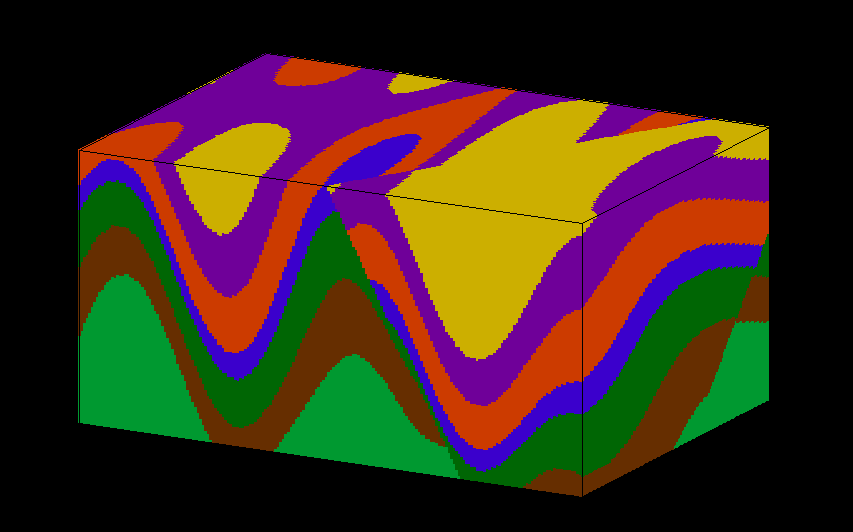
\includegraphics{noddy_block_example.png}
\end{figure}

\code{Noddy} has been used to generate models for teaching and
interpretation purposes, but also for scientific studies (e.g. {[}3{]}).

<<<<<<< HEAD
\href{https://github.com/markjessell/functionNoddy}{https://github.com/markjessell/functionNoddy}
=======
>>>>>>> refs/remotes/flohorovicic/master

\section{Installation}
\label{readme:installation}

\section{Installation of the \texttt{pynoddy} package}
\label{readme:installation-of-the-pynoddy-package}
A successful installation of \code{pynoddy} requires two steps:
\begin{enumerate}
\item {} 
An installation of the python modules in the package \code{pynoddy}

<<<<<<< HEAD
\section{References}
\label{readme:references}
{[}1{]} Mark W. Jessell, Rick K. Valenta, Structural geophysics: Integrated
structural and geophysical modelling, In: Declan G. De Paor, Editor(s),
Computer Methods in the Geosciences, Pergamon, 1996, Volume 15, Pages
303-324, ISSN 1874-561X, ISBN 9780080424309,
\href{http://dx.doi.org/10.1016/S1874-561X(96)80027-7}{http://dx.doi.org/10.1016/S1874-561X(96)80027-7}.
=======
\item {} 
The existance of an executable \code{Noddy(.exe)} program
>>>>>>> refs/remotes/flohorovicic/master

\end{enumerate}

Installation of the first part is straight-forward:

For the best (and most complete) installation, we suggest to clone the
\code{pynoddy} repository on:

\href{https://github.com/flohorovicic/pynoddy}{https://github.com/flohorovicic/pynoddy}

To install \code{pynoddy} simply run:

\begin{Verbatim}[commandchars=\\\{\}]
python setup.py install
\end{Verbatim}

sufficient privileges are required (i.e. run in \code{sudo} with MacOSX/
Linux and set permissions on Windows)

The pynoddy packages themselves can also be installed directly from the
Python Package Index (pypi.org) via pip:

\begin{Verbatim}[commandchars=\\\{\}]
pip install pynoddy
\end{Verbatim}

A Windows installer is also available on the Pypi page:

\href{https://pypi.python.org/pypi/pynoddy/}{https://pypi.python.org/pypi/pynoddy/}


\section{Installation of \texttt{Noddy}}
\label{readme:installation-of-noddy}
\code{Noddy} is a command line program, written in C, that performs the
kinematic simulation itself. The program compilation is platform
dependent, and therefore several ways for installation are possible (see
below information for specific platforms).


\section{Using a pre-compiled version of \texttt{Noddy}}
\label{readme:using-a-pre-compiled-version-of-noddy}
The easy way to obtain a executable version of \code{Noddy} is simply to
download the appropriate version for your operating system. Currently,
these executables versions are also stored on github (check the
up-to-date online documentation if this should not anymore be the case)
in the directory:

\href{https://github.com/flohorovicic/pynoddy/tree/master/noddyapp}{https://github.com/flohorovicic/pynoddy/tree/master/noddyapp}

Furthermore, the executables for Windows are also available for download
on the webpage:

\href{http://www.tectonique.net/pynoddy}{http://www.tectonique.net/pynoddy}

Download the appropriate app, rename it to \code{noddy} or \code{noddy.exe}
and place it into a folder that is in your local environment path
variable. If you are not sure if a folder is in the \code{PATH} or would
like to add new one, see below for more information.


\section{Compiling \texttt{Noddy} from source files (recommended installation)}
\label{readme:compiling-noddy-from-source-files-recommended-installation}
The source code for the executable \code{Noddy} is located in the
repository directory \code{noddy}. In order to perform the installation, a
\code{gcc} compiler is required. This compiler should be available on Linux
and MacOSX operating systems. On Windows, one possibility is to install
MinGW. Otherwise, the code requires no specific libraries.

Note for MacOSX users: some header files have to be adapted to avoid
conflicts with local libraries. The required adaptations are executed
when running the script:

\begin{Verbatim}[commandchars=\\\{\}]
\PYGZgt{} adjust\PYGZus{}for\PYGZus{}MacOSX.sh
\end{Verbatim}

The compilation is then performed (in a Linux, MacOSX, or Windows MinGW
terminal) with the command:

\begin{Verbatim}[commandchars=\\\{\}]
\PYGZgt{} compile.sh
\end{Verbatim}

Compilation usually produces multiple warnings, but should otherwise
proceed successfully.


\section{Placing the executable \texttt{noddy} in the Path}
\label{readme:placing-the-executable-noddy-in-the-path}
For the most general installation, the executable of \code{Noddy} should be
placed in a folder that can be located from any terminal application in
the system. This (usually) means that the folder with the executable has
to be in the \code{PATH} environment variable. On Linux and MacOSX, a path
can simply be added by:

\begin{Verbatim}[commandchars=\\\{\}]
\PYGZgt{} export PATH\PYGZhy{}\PYGZdq{}path/to/executable/:\PYGZbs{}\PYGZdl{}PATH\PYGZdq{}
\end{Verbatim}

Note that this command should be placed into your .bash\_profile file to
ensure that the path is added whenever you start a new Python script.

On \code{windows}, adding a folder to the local environment variable
\code{Path} is usually done through the System Control Panel (Start -
Settings - Control Panel - System). in Advanced mode, open the
Environment Variables sub-menu, and find the variable Path. Click to
edit the variable, and add the location of your folder to this path.


\section{Noddy executable and GUI for Windows}
\label{readme:noddy-executable-and-gui-for-windows}
The original graphical user interface for \code{Noddy} and the compiled
executable program for Windows can be obtained from:

\href{http://tinyurl.com/noddy-site}{http://tinyurl.com/noddy-site}

This site also contains the source code, as well as extensive
documentation and tutorial material concerning the original
implementation of the software, as well as more technical details on the
modelling method itself.


\section{Testing the installation}
\label{readme:testing-the-installation}

\section{Testing \texttt{noddy}}
\label{readme:testing-noddy}
Simply test the installation by running the generated (or downloaded)
executable in a terminal window (on Windows: \code{cmd}):

\begin{Verbatim}[commandchars=\\\{\}]
\PYGZgt{} noddy
\end{Verbatim}

or (depending on your compilation or naming convention):

\begin{Verbatim}[commandchars=\\\{\}]
\PYGZgt{} noddy.exe
\end{Verbatim}

Which should produce the general output:

\begin{Verbatim}[commandchars=\\\{\}]
Arguments \PYGZlt{}historyfile\PYGZgt{} \PYGZlt{}outputfile\PYGZgt{} \PYGZlt{}calc\PYGZus{}mode\PYGZgt{}:
BLOCK
GEOPHYSICS
SURFACES
BLOCK\PYGZus{}GEOPHYS
BLOCK\PYGZus{}SURFACES
TOPOLOGY
ANOM\PYGZus{}FROM\PYGZus{}BLOCK
ALL
\end{Verbatim}

Note: if the executable is correctly placed in a folder which is
recognised by the (Environment) path variable, then you should be able
to run \code{Noddy} from any directory. If this is not the case, please
check if it is correctly placed in the path (see above).


\section{Testing \texttt{pynoddy}}
\label{readme:testing-pynoddy}
The \code{pynoddy} package contains a set of tests which can be executed in
the standard Python testing environment. If you cloned or downloaded the
repository, then these tests can directly be performed through the setup
script:

\begin{Verbatim}[commandchars=\\\{\}]
\PYGZgt{} python setup.py test
\end{Verbatim}

Of specific relevance is the test that determines if the \code{noddy(.exe)}
executable is correctly accessible from \code{pynoddy}. If this is the
case, then the \code{compute\_model} test should return:

\begin{Verbatim}[commandchars=\\\{\}]
test\PYGZus{}compute\PYGZus{}model (test.TestHistory) ... ok\PYGZcb{}
\end{Verbatim}

If this test is not ok, then please check carefully the installation of
the \code{noddy(.exe)} executable.

If all tests are successful, \textbf{you are ready to go!}


\section{How to get started}
\label{readme:how-to-get-started}

\section{Tutorial Jupyter notebooks}
\label{readme:tutorial-jupyter-notebooks}
The best way to get started with \code{pynoddy} is to have a look at the
IPython notebooks in pynoddy/docs/notebooks. The numbered notebooks are
those that are part of the documentation, and a good point to get
started.

The notebooks require an installed Jupyter notebook. More information
here:

\href{https://jupyter.org}{https://jupyter.org}

The notebook can be installed via \code{pip} or \code{conda}.


\section{The Atlas of Strutural Geophysics}
\label{readme:the-atlas-of-strutural-geophysics}
The Atlas of Structural Geophysics contains a collection of structural
models, together with their expression as geophysical potential fields
(gravity and magnetics), with a focus on guiding the interpretation of
observed features in potential-field maps.

The atlas is currently available on:

\href{http://tectonique.net/asg}{http://tectonique.net/asg}

The structural models are created with Noddy and the history files can
be downloaded from the atlas. Models from this Atlas can directly be
loaded with \code{pynoddy}. See example notebooks and documentation for
more details.


\section{Documentation}
\label{readme:documentation}
An updated version of the documentation is available within the
\code{pynoddy} repository (pynoddy/docs).

In addition, an online html version of the documentation is also hosted
on readthedocs:

\href{http://pynoddy.readthedocs.org}{http://pynoddy.readthedocs.org}


\section{Technical Notes}
\label{readme:technical-notes}

\section{Dependencies}
\label{readme:dependencies}
\code{pynoddy} depends on several standard Python packages that should be
shipped with any standard distribution (and are easy to install,
otherwise):
\begin{itemize}
\item {} 
numpy

\item {} 
matplotlib

\item {} 
pickle

\end{itemize}

The uncertainty analysis, quantification, and visualisation methods
based on information theory are implemented in the python package
pygeoinfo. This package is available on github and part of the python
package index. It is automatically installed with the setup script
provided with this package.

In addition, to export model results for full 3-D visualisation with
VTK, the pyevtk package is used, available on bitbucket:

\href{https://bitbucket.org/pauloh/pyevtk/src/9c19e3a54d1e?at-v0.1.0}{https://bitbucket.org/pauloh/pyevtk/src/9c19e3a54d1e?at-v0.1.0}

The package is automatically downloaded and installed when running
python setup.py install.


\section{3-D Visualisation}
\label{readme:d-visualisation}
At this stage, we do not supply methods for 3-D visualisation in python
(although this may change in the future). However, we provide methods to
export results into a VTK format. Exported files can then be viewed with
the highly functional VTK viewers, and several free options are
available, for example:
\begin{itemize}
\item {} 
Paraview: \href{http://www.paraview.org}{http://www.paraview.org}

\item {} 
Visit: \href{https://wci.llnl.gov/simulation/computer-codes/visit/}{https://wci.llnl.gov/simulation/computer-codes/visit/}

\item {} 
Mayavi: \href{http://docs.enthought.com/mayavi/mayavi/}{http://docs.enthought.com/mayavi/mayavi/}

\end{itemize}

License
\textasciitilde{}\textasciitilde{}\textasciitilde{}\textasciitilde{}\textasciitilde{}\textasciitilde{}-

\code{pynoddy} is free software (see license file included in the
repository). Please attribute the work when you use it and cite the
publication if you use it in a scientific context - feel free to change
and adapt it otherwise!


\section{References}
\label{readme:references}
{[}1{]} Mark W. Jessell. Noddy, an interactive map creation package.
Unpublished MSc Thesis, University of London. 1981.

{[}2{]} Mark W. Jessell, Rick K. Valenta, Structural geophysics: Integrated
structural and geophysical modelling, In: Declan G. De Paor, Editor(s),
Computer Methods in the Geosciences, Pergamon, 1996, Volume 15, Pages
303-324, ISSN 1874-561X, ISBN 9780080424309,
\href{http://dx.doi.org/10.1016/S1874-561X(96)80027-7}{http://dx.doi.org/10.1016/S1874-561X(96)80027-7}.

{[}3{]} Armit, R. J., Betts, P. G., Schaefer, B. F., \& Ailleres, L. (2012).
Constraints on long-lived Mesoproterozoic and Palaeozoic deformational
events and crustal architecture in the northern Mount Painter Province,
Australia. Gondwana Research, 22(1), 207–226.
\href{http://doi.org/10.1016/j.gr.2011.11.003}{http://doi.org/10.1016/j.gr.2011.11.003}


\chapter{pynoddy.noddy module}
\label{noddy_module::doc}\label{noddy_module:pynoddy-noddy-module}
This module contains the Noddy code that is actually used to compute the kinematic models
defined in .his files.

Note that this code \emph{must be compiled} before \code{pynoddy.compute\_model}
will function correctly. It should compile easily (plus or minus a few thousand
warnings) using the \code{compile.sh} script. Windows users will first need to install the GCC
library (e.g. through MinGW), but otherwise the code requires no non-standard libraries.

\textbf{Usage}

The compiled noddy code can be run directly from the command line to a realisation of a model
defined in a .his file, or called through \code{pynoddy.compute\_model}.

If the binary is called from the command line it takes the following arguments:

\begin{Verbatim}[commandchars=\\\{\}]
\PYG{n}{noddy} \PYG{p}{[}\PYG{n}{history\PYGZus{}file}\PYG{p}{]} \PYG{p}{[}\PYG{n}{output\PYGZus{}name}\PYG{p}{]} \PYG{p}{[}\PYG{n}{calculation\PYGZus{}mode}\PYG{p}{]}
\end{Verbatim}
\begin{description}
\item[{Where:}] \leavevmode\begin{itemize}
\item {} 
\code{history\_file} is the filepath (including the extension) of the .his file defining the model

\item {} 
\code{output\_name} is the name that will be assigned to the noddy output files

\end{itemize}

\item[{The \code{mode} argument determines the type of output that noddy generates, and can be any one of:}] \leavevmode\begin{itemize}
\item {} 
BLOCK - calculates the lithology block model

\item {} 
GEOPHYSICS - calculates the geophysical expression (magnetics and gravity) of the model

\item {} 
SURFACES - calculates surfaces representing the lithological contacts

\item {} 
BLOCK\_GEOPHYS - calculates the lithology block model and its geophysical expression

\item {} 
BLOCK\_SURFACES - calculates the lithology block model and lithological surfaces

\item {} 
TOPOLOGY - calculates the lithology block model and associated topology information

\item {} 
ANOM\_FROM\_BLOCK - calculates the geophysical expression of an existing lithology block (output\_name.g12)

\item {} 
ALL - calculates the block, geophysics, topology and surfaces

\end{itemize}

\end{description}

\textbf{Python Wrapper}

As mentioned earlier, the executable can also be accessed from python via pynoddy.
This is performed by calling the \code{pynoddy.compute\_model} function, as defined below:
\index{compute\_model() (in module pynoddy)}

\begin{fulllineitems}
\phantomsection\label{noddy_module:pynoddy.compute_model}\pysiglinewithargsret{\code{pynoddy.}\bfcode{compute\_model}}{\emph{history}, \emph{output\_name}, \emph{**kwds}}{}
Call Noddy and compute the history file
\begin{description}
\item[{\textbf{Arguments}:}] \leavevmode\begin{itemize}
\item {} 
\emph{history} = string : filename of history file

\item {} 
\emph{output\_name} = string : basename for output files

\end{itemize}

\item[{\textbf{Optional Keywords}:}] \leavevmode\begin{itemize}
\item {} 
\emph{sim\_type} = `BLOCK', `GEOPHYSICS', `SURFACES', `BLOCK\_GEOPHYS',

\end{itemize}
\begin{description}
\item[{`TOPOLOGY', `BLOCK\_SURFACES', `ALL':}] \leavevmode
type of Noddy simulation (default: `BLOCK')

\end{description}
\begin{itemize}
\item {} \begin{description}
\item[{\emph{program\_name} = string}] \leavevmode{[}name of program{]}
(default: noddy.exe or noddy, both checked)

\end{description}

\item {} 
\emph{verbose} = bool: verbose mode, print out information for debugging (default = False)

\item {} 
\emph{noddy\_path} = path: location of Noddy executable (default: checks environment variable)

\end{itemize}

\item[{\textbf{Returns}:}] \leavevmode
-Returns any text outputted by the noddy executable.

\end{description}

\end{fulllineitems}


It is worth noting here that by default pynoddy looks for the compiled Noddy executable in the pynoddy.noddy directory. However
this can be changed by updating the \code{pynoddy.noddyPath} variable to point to a new executable file (without any extension, .exe
is added automatically to the path on windows machines).


\chapter{Simulation of a Noddy history and visualisation of output}
\label{notebooks/1-Simulation:simulation-of-a-noddy-history-and-visualisation-of-output}\label{notebooks/1-Simulation::doc}
This example shows how the module pynoddy.history can be used to compute
the model, and how simple visualisations can be generated with
pynoddy.output.

\begin{Verbatim}[commandchars=\\\{\}]
\PYG{k+kn}{from} \PYG{n+nn}{IPython.core.display} \PYG{k+kn}{import} \PYG{n}{HTML}
\PYG{n}{css\PYGZus{}file} \PYG{o}{=} \PYG{l+s}{\PYGZsq{}}\PYG{l+s}{pynoddy.css}\PYG{l+s}{\PYGZsq{}}
\PYG{n}{HTML}\PYG{p}{(}\PYG{n+nb}{open}\PYG{p}{(}\PYG{n}{css\PYGZus{}file}\PYG{p}{,} \PYG{l+s}{\PYGZdq{}}\PYG{l+s}{r}\PYG{l+s}{\PYGZdq{}}\PYG{p}{)}\PYG{o}{.}\PYG{n}{read}\PYG{p}{(}\PYG{p}{)}\PYG{p}{)}
\end{Verbatim}

\begin{Verbatim}[commandchars=\\\{\}]
\PYGZpc{}matplotlib inline
\end{Verbatim}

\begin{Verbatim}[commandchars=\\\{\}]
\PYG{c}{\PYGZsh{} Basic settings}
\PYG{k+kn}{import} \PYG{n+nn}{sys}\PYG{o}{,} \PYG{n+nn}{os}
\PYG{k+kn}{import} \PYG{n+nn}{subprocess}

\PYG{c}{\PYGZsh{} Now import pynoddy}
\PYG{k+kn}{import} \PYG{n+nn}{pynoddy}
\PYG{n+nb}{reload}\PYG{p}{(}\PYG{n}{pynoddy}\PYG{p}{)}
\PYG{k+kn}{import} \PYG{n+nn}{pynoddy.output}
\PYG{k+kn}{import} \PYG{n+nn}{pynoddy.history}

\PYG{c}{\PYGZsh{} determine path of repository to set paths corretly below}
\PYG{n}{repo\PYGZus{}path} \PYG{o}{=} \PYG{n}{os}\PYG{o}{.}\PYG{n}{path}\PYG{o}{.}\PYG{n}{realpath}\PYG{p}{(}\PYG{l+s}{\PYGZsq{}}\PYG{l+s}{../..}\PYG{l+s}{\PYGZsq{}}\PYG{p}{)}
\end{Verbatim}


\section{Compute the model}
\label{notebooks/1-Simulation:compute-the-model}
The simplest way to perform the Noddy simulation through Python is
simply to call the executable. One way that should be fairly platform
independent is to use Python's own subprocess module:

\begin{Verbatim}[commandchars=\\\{\}]
\PYG{c}{\PYGZsh{} Change to sandbox directory to store results}
\PYG{n}{os}\PYG{o}{.}\PYG{n}{chdir}\PYG{p}{(}\PYG{n}{os}\PYG{o}{.}\PYG{n}{path}\PYG{o}{.}\PYG{n}{join}\PYG{p}{(}\PYG{n}{repo\PYGZus{}path}\PYG{p}{,} \PYG{l+s}{\PYGZsq{}}\PYG{l+s}{sandbox}\PYG{l+s}{\PYGZsq{}}\PYG{p}{)}\PYG{p}{)}

\PYG{c}{\PYGZsh{} Path to exmaple directory in this repository}
\PYG{n}{example\PYGZus{}directory} \PYG{o}{=} \PYG{n}{os}\PYG{o}{.}\PYG{n}{path}\PYG{o}{.}\PYG{n}{join}\PYG{p}{(}\PYG{n}{repo\PYGZus{}path}\PYG{p}{,}\PYG{l+s}{\PYGZsq{}}\PYG{l+s}{examples}\PYG{l+s}{\PYGZsq{}}\PYG{p}{)}
\PYG{c}{\PYGZsh{} Compute noddy model for history file}
\PYG{n}{history\PYGZus{}file} \PYG{o}{=} \PYG{l+s}{\PYGZsq{}}\PYG{l+s}{simple\PYGZus{}two\PYGZus{}faults.his}\PYG{l+s}{\PYGZsq{}}
\PYG{n}{history} \PYG{o}{=} \PYG{n}{os}\PYG{o}{.}\PYG{n}{path}\PYG{o}{.}\PYG{n}{join}\PYG{p}{(}\PYG{n}{example\PYGZus{}directory}\PYG{p}{,} \PYG{n}{history\PYGZus{}file}\PYG{p}{)}
\PYG{n}{output\PYGZus{}name} \PYG{o}{=} \PYG{l+s}{\PYGZsq{}}\PYG{l+s}{noddy\PYGZus{}out}\PYG{l+s}{\PYGZsq{}}
\PYG{c}{\PYGZsh{} call Noddy}

\PYG{c}{\PYGZsh{} NOTE: Make sure that the noddy executable is accessible in the system!!}
\PYG{k}{print} \PYG{n}{subprocess}\PYG{o}{.}\PYG{n}{Popen}\PYG{p}{(}\PYG{p}{[}\PYG{l+s}{\PYGZsq{}}\PYG{l+s}{noddy.exe}\PYG{l+s}{\PYGZsq{}}\PYG{p}{,} \PYG{n}{history}\PYG{p}{,} \PYG{n}{output\PYGZus{}name}\PYG{p}{,} \PYG{l+s}{\PYGZsq{}}\PYG{l+s}{BLOCK}\PYG{l+s}{\PYGZsq{}}\PYG{p}{]}\PYG{p}{,}
                       \PYG{n}{shell}\PYG{o}{=}\PYG{n+nb+bp}{False}\PYG{p}{,} \PYG{n}{stderr}\PYG{o}{=}\PYG{n}{subprocess}\PYG{o}{.}\PYG{n}{PIPE}\PYG{p}{,}
                       \PYG{n}{stdout}\PYG{o}{=}\PYG{n}{subprocess}\PYG{o}{.}\PYG{n}{PIPE}\PYG{p}{)}\PYG{o}{.}\PYG{n}{stdout}\PYG{o}{.}\PYG{n}{read}\PYG{p}{(}\PYG{p}{)}
\PYG{c}{\PYGZsh{}}
\end{Verbatim}

For convenience, the model computation is wrapped into a Python function
in pynoddy:

\begin{Verbatim}[commandchars=\\\{\}]
\PYG{n}{pynoddy}\PYG{o}{.}\PYG{n}{compute\PYGZus{}model}\PYG{p}{(}\PYG{n}{history}\PYG{p}{,} \PYG{n}{output\PYGZus{}name}\PYG{p}{)}
\end{Verbatim}

\begin{Verbatim}[commandchars=\\\{\}]
\PYG{l+s}{\PYGZsq{}}\PYG{l+s}{\PYGZsq{}}
\end{Verbatim}

Note: The Noddy call from Python is, to date, calling Noddy through the
subprocess function. In a future implementation, this call could be
substituted with a full wrapper for the C-functions written in Python.
Therefore, using the member function compute\_model is not only easier,
but also the more ``future-proof'' way to compute the Noddy model.


\section{Loading Noddy output files}
\label{notebooks/1-Simulation:loading-noddy-output-files}
Noddy simulations produce a variety of different output files, depending
on the type of simulation. The basic output is the geological model.
Additional output files can contain geophysical responses, etc.

Loading the output files is simplified with a class class container that
reads all relevant information and provides simple methods for plotting,
model analysis, and export. To load the output information into a Python
object:

\begin{Verbatim}[commandchars=\\\{\}]
\PYG{n}{N1} \PYG{o}{=} \PYG{n}{pynoddy}\PYG{o}{.}\PYG{n}{output}\PYG{o}{.}\PYG{n}{NoddyOutput}\PYG{p}{(}\PYG{n}{output\PYGZus{}name}\PYG{p}{)}
\end{Verbatim}

The object contains the calculated geology blocks and some additional
information on grid spacing, model extent, etc. For example:

\begin{Verbatim}[commandchars=\\\{\}]
\PYG{k}{print}\PYG{p}{(}\PYG{l+s}{\PYGZdq{}}\PYG{l+s}{The model has an extent of }\PYG{l+s+si}{\PYGZpc{}.0f}\PYG{l+s}{ m in x\PYGZhy{}direction, with }\PYG{l+s+si}{\PYGZpc{}d}\PYG{l+s}{ cells of width }\PYG{l+s+si}{\PYGZpc{}.0f}\PYG{l+s}{ m}\PYG{l+s}{\PYGZdq{}} \PYG{o}{\PYGZpc{}}
      \PYG{p}{(}\PYG{n}{N1}\PYG{o}{.}\PYG{n}{extent\PYGZus{}x}\PYG{p}{,} \PYG{n}{N1}\PYG{o}{.}\PYG{n}{nx}\PYG{p}{,} \PYG{n}{N1}\PYG{o}{.}\PYG{n}{delx}\PYG{p}{)}\PYG{p}{)}
\end{Verbatim}

\begin{Verbatim}[commandchars=\\\{\}]
The model has an extent of 12400 m in x\PYGZhy{}direction, with 124 cells of width 100 m
\end{Verbatim}


\section{Plotting sections through the model}
\label{notebooks/1-Simulation:plotting-sections-through-the-model}
The NoddyOutput class has some basic methods for the visualisation of
the generated models. To plot sections through the model:

\begin{Verbatim}[commandchars=\\\{\}]
\PYG{n}{N1}\PYG{o}{.}\PYG{n}{plot\PYGZus{}section}\PYG{p}{(}\PYG{l+s}{\PYGZsq{}}\PYG{l+s}{y}\PYG{l+s}{\PYGZsq{}}\PYG{p}{,} \PYG{n}{figsize} \PYG{o}{=} \PYG{p}{(}\PYG{l+m+mi}{5}\PYG{p}{,}\PYG{l+m+mi}{3}\PYG{p}{)}\PYG{p}{)}
\end{Verbatim}

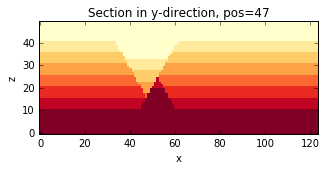
\includegraphics{1-Simulation_14_0.png}


\section{Export model to VTK}
\label{notebooks/1-Simulation:export-model-to-vtk}
A simple possibility to visualise the modeled results in 3-D is to
export the model to a VTK file and then to visualise it with a VTK
viewer, for example Paraview. To export the model, simply use:

\begin{Verbatim}[commandchars=\\\{\}]
\PYG{n}{N1}\PYG{o}{.}\PYG{n}{export\PYGZus{}to\PYGZus{}vtk}\PYG{p}{(}\PYG{p}{)}
\end{Verbatim}

The exported VTK file can be visualised in any VTK viewer, for example
in the (free) viewer Paraview (www.paraview.org). An example
visualisation of the model in 3-D is presented in the figure below.
\begin{figure}[htbp]
\centering
\capstart

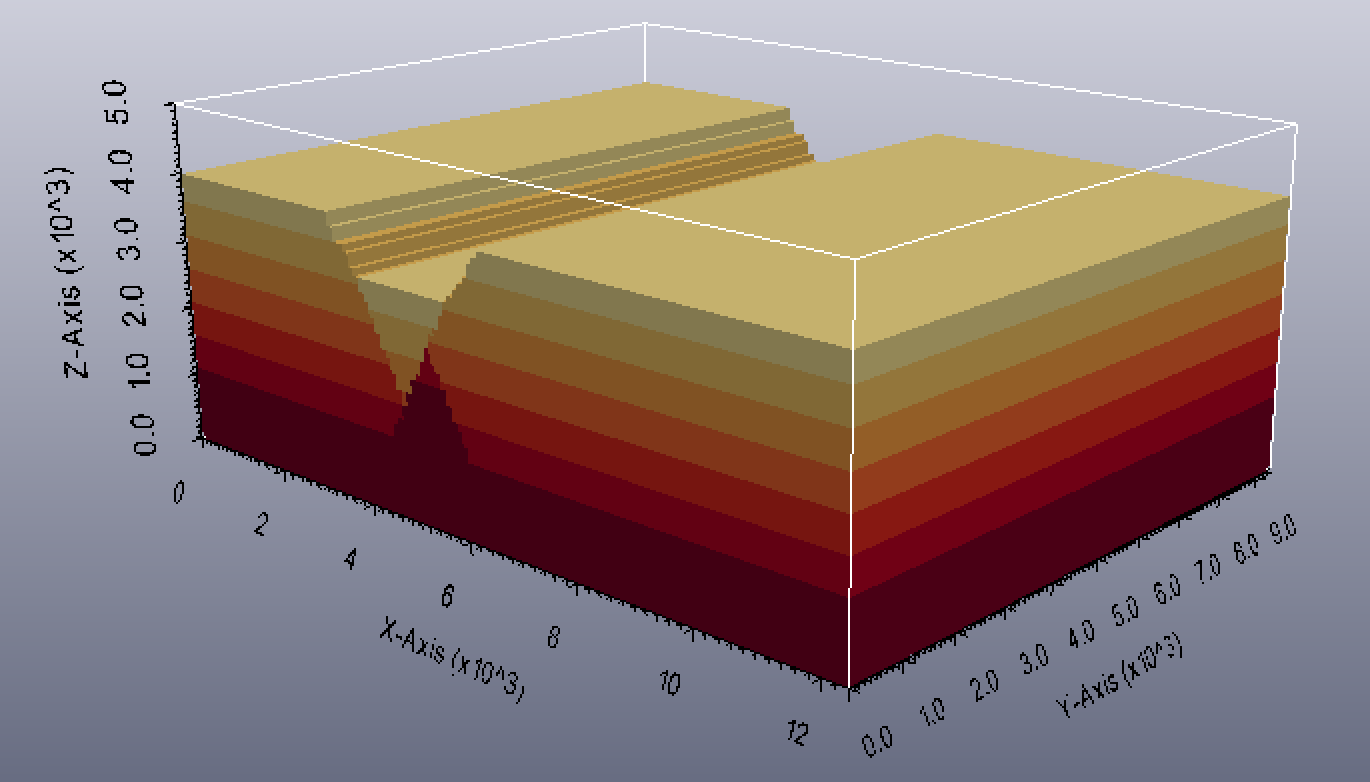
\includegraphics{3d_render_fault_model_2.png}
\caption{3-D Visualisation generated with Paraview (top layer transparent)}\end{figure}


\chapter{Change Noddy input file and recompute model}
\label{notebooks/2-Adjust-input::doc}\label{notebooks/2-Adjust-input:change-noddy-input-file-and-recompute-model}
In this section, we will briefly present possibilities to access the
properties defined in the Noddy history input file and show how simple
adjustments can be performed, for example changing the cube size to
obtain a model with a higher resolution.

Also outlined here is the way that events are stored in the history file
as single objects. For more information on accessing and changing the
events themselves, please be patient until we get to the next section.

\begin{Verbatim}[commandchars=\\\{\}]
\PYG{k+kn}{from} \PYG{n+nn}{IPython.core.display} \PYG{k+kn}{import} \PYG{n}{HTML}
\PYG{n}{css\PYGZus{}file} \PYG{o}{=} \PYG{l+s}{\PYGZsq{}}\PYG{l+s}{pynoddy.css}\PYG{l+s}{\PYGZsq{}}
\PYG{n}{HTML}\PYG{p}{(}\PYG{n+nb}{open}\PYG{p}{(}\PYG{n}{css\PYGZus{}file}\PYG{p}{,} \PYG{l+s}{\PYGZdq{}}\PYG{l+s}{r}\PYG{l+s}{\PYGZdq{}}\PYG{p}{)}\PYG{o}{.}\PYG{n}{read}\PYG{p}{(}\PYG{p}{)}\PYG{p}{)}
\end{Verbatim}

\begin{Verbatim}[commandchars=\\\{\}]
cd ../docs/notebooks/
\end{Verbatim}

\begin{Verbatim}[commandchars=\\\{\}]
/Users/flow/git/pynoddy/docs/notebooks
\end{Verbatim}

\begin{Verbatim}[commandchars=\\\{\}]
\PYGZpc{}matplotlib inline
\end{Verbatim}

\begin{Verbatim}[commandchars=\\\{\}]
\PYG{k+kn}{import} \PYG{n+nn}{sys}\PYG{o}{,} \PYG{n+nn}{os}
\PYG{k+kn}{import} \PYG{n+nn}{matplotlib.pyplot} \PYG{k+kn}{as} \PYG{n+nn}{plt}
\PYG{k+kn}{import} \PYG{n+nn}{numpy} \PYG{k+kn}{as} \PYG{n+nn}{np}
\PYG{c}{\PYGZsh{} adjust some settings for matplotlib}
\PYG{k+kn}{from} \PYG{n+nn}{matplotlib} \PYG{k+kn}{import} \PYG{n}{rcParams}
\PYG{c}{\PYGZsh{} print rcParams}
\PYG{n}{rcParams}\PYG{p}{[}\PYG{l+s}{\PYGZsq{}}\PYG{l+s}{font.size}\PYG{l+s}{\PYGZsq{}}\PYG{p}{]} \PYG{o}{=} \PYG{l+m+mi}{15}
\PYG{c}{\PYGZsh{} determine path of repository to set paths corretly below}
\PYG{n}{repo\PYGZus{}path} \PYG{o}{=} \PYG{n}{os}\PYG{o}{.}\PYG{n}{path}\PYG{o}{.}\PYG{n}{realpath}\PYG{p}{(}\PYG{l+s}{\PYGZsq{}}\PYG{l+s}{../..}\PYG{l+s}{\PYGZsq{}}\PYG{p}{)}
\PYG{k+kn}{import} \PYG{n+nn}{pynoddy}
\PYG{k+kn}{import} \PYG{n+nn}{pynoddy.history}
\PYG{k+kn}{import} \PYG{n+nn}{pynoddy.output}
\end{Verbatim}

First step: load the history file into a Python object:

\begin{Verbatim}[commandchars=\\\{\}]
\PYG{c}{\PYGZsh{} Change to sandbox directory to store results}
\PYG{n}{os}\PYG{o}{.}\PYG{n}{chdir}\PYG{p}{(}\PYG{n}{os}\PYG{o}{.}\PYG{n}{path}\PYG{o}{.}\PYG{n}{join}\PYG{p}{(}\PYG{n}{repo\PYGZus{}path}\PYG{p}{,} \PYG{l+s}{\PYGZsq{}}\PYG{l+s}{sandbox}\PYG{l+s}{\PYGZsq{}}\PYG{p}{)}\PYG{p}{)}
\PYG{c}{\PYGZsh{} Path to exmaple directory in this repository}
\PYG{n}{example\PYGZus{}directory} \PYG{o}{=} \PYG{n}{os}\PYG{o}{.}\PYG{n}{path}\PYG{o}{.}\PYG{n}{join}\PYG{p}{(}\PYG{n}{repo\PYGZus{}path}\PYG{p}{,}\PYG{l+s}{\PYGZsq{}}\PYG{l+s}{examples}\PYG{l+s}{\PYGZsq{}}\PYG{p}{)}
\PYG{c}{\PYGZsh{} Compute noddy model for history file}
\PYG{n}{history\PYGZus{}file} \PYG{o}{=} \PYG{l+s}{\PYGZsq{}}\PYG{l+s}{simple\PYGZus{}two\PYGZus{}faults.his}\PYG{l+s}{\PYGZsq{}}
\PYG{n}{history} \PYG{o}{=} \PYG{n}{os}\PYG{o}{.}\PYG{n}{path}\PYG{o}{.}\PYG{n}{join}\PYG{p}{(}\PYG{n}{example\PYGZus{}directory}\PYG{p}{,} \PYG{n}{history\PYGZus{}file}\PYG{p}{)}
\PYG{n}{output\PYGZus{}name} \PYG{o}{=} \PYG{l+s}{\PYGZsq{}}\PYG{l+s}{noddy\PYGZus{}out}\PYG{l+s}{\PYGZsq{}}
\PYG{n}{H1} \PYG{o}{=} \PYG{n}{pynoddy}\PYG{o}{.}\PYG{n}{history}\PYG{o}{.}\PYG{n}{NoddyHistory}\PYG{p}{(}\PYG{n}{history}\PYG{p}{)}
\end{Verbatim}

\textbf{Technical note}: the \code{NoddyHistory} class can be accessed on the
level of pynoddy (as it is imported in the \code{\_\_init\_\_.py} module) with
the shortcut:

\code{H1 = pynoddy.NoddyHistory(history)}

I am using the long version \code{pynoddy.history.NoddyHistory} here to
ensure that the correct package is loaded with the \code{reload()}
function. If you don't make changes to any of the pynoddy files, this is
not required. So for any practical cases, the shortcuts are absolutely
fine!


\section{Get basic information on the model}
\label{notebooks/2-Adjust-input:get-basic-information-on-the-model}
The history file contains the entire information on the Noddy model.
Some information can be accessed through the NoddyHistory object (and
more will be added soon!), for example the total number of events:

\begin{Verbatim}[commandchars=\\\{\}]
\PYG{k}{print}\PYG{p}{(}\PYG{l+s}{\PYGZdq{}}\PYG{l+s}{The history contains }\PYG{l+s+si}{\PYGZpc{}d}\PYG{l+s}{ events}\PYG{l+s}{\PYGZdq{}} \PYG{o}{\PYGZpc{}} \PYG{n}{H1}\PYG{o}{.}\PYG{n}{n\PYGZus{}events}\PYG{p}{)}
\end{Verbatim}

\begin{Verbatim}[commandchars=\\\{\}]
The history contains 3 events
\end{Verbatim}

Events are implemented as objects, the classes are defined in
\code{H1.events}. All events are accessible in a list on the level of the
history object:

\begin{Verbatim}[commandchars=\\\{\}]
\PYG{n}{H1}\PYG{o}{.}\PYG{n}{events}
\end{Verbatim}

\begin{Verbatim}[commandchars=\\\{\}]
\PYGZob{}1: \PYGZlt{}pynoddy.events.Stratigraphy at 0x103ac2a50\PYGZgt{},
 2: \PYGZlt{}pynoddy.events.Fault at 0x103ac2a90\PYGZgt{},
 3: \PYGZlt{}pynoddy.events.Fault at 0x103ac2ad0\PYGZgt{}\PYGZcb{}
\end{Verbatim}

The properties of an event are stored in the event objects themselves.
To date, only a subset of the properties (deemed as relevant for the
purpose of pynoddy so far) are parsed. The .his file contains a lot more
information! If access to this information is required, adjustments in
pynoddy.events have to be made.

For example, the properties of a fault object are:

\begin{Verbatim}[commandchars=\\\{\}]
\PYG{n}{H1}\PYG{o}{.}\PYG{n}{events}\PYG{p}{[}\PYG{l+m+mi}{2}\PYG{p}{]}\PYG{o}{.}\PYG{n}{properties}
\PYG{c}{\PYGZsh{} print H1.events[5].properties.keys()}
\end{Verbatim}

\begin{Verbatim}[commandchars=\\\{\}]
\PYG{p}{\PYGZob{}}\PYG{l+s}{\PYGZsq{}}\PYG{l+s}{Amplitude}\PYG{l+s}{\PYGZsq{}}\PYG{p}{:} \PYG{l+m+mf}{2000.0}\PYG{p}{,}
 \PYG{l+s}{\PYGZsq{}}\PYG{l+s}{Blue}\PYG{l+s}{\PYGZsq{}}\PYG{p}{:} \PYG{l+m+mf}{254.0}\PYG{p}{,}
 \PYG{l+s}{\PYGZsq{}}\PYG{l+s}{Color Name}\PYG{l+s}{\PYGZsq{}}\PYG{p}{:} \PYG{l+s}{\PYGZsq{}}\PYG{l+s}{Custom Colour 8}\PYG{l+s}{\PYGZsq{}}\PYG{p}{,}
 \PYG{l+s}{\PYGZsq{}}\PYG{l+s}{Cyl Index}\PYG{l+s}{\PYGZsq{}}\PYG{p}{:} \PYG{l+m+mf}{0.0}\PYG{p}{,}
 \PYG{l+s}{\PYGZsq{}}\PYG{l+s}{Dip}\PYG{l+s}{\PYGZsq{}}\PYG{p}{:} \PYG{l+m+mf}{60.0}\PYG{p}{,}
 \PYG{l+s}{\PYGZsq{}}\PYG{l+s}{Dip Direction}\PYG{l+s}{\PYGZsq{}}\PYG{p}{:} \PYG{l+m+mf}{90.0}\PYG{p}{,}
 \PYG{l+s}{\PYGZsq{}}\PYG{l+s}{Geometry}\PYG{l+s}{\PYGZsq{}}\PYG{p}{:} \PYG{l+s}{\PYGZsq{}}\PYG{l+s}{Translation}\PYG{l+s}{\PYGZsq{}}\PYG{p}{,}
 \PYG{l+s}{\PYGZsq{}}\PYG{l+s}{Green}\PYG{l+s}{\PYGZsq{}}\PYG{p}{:} \PYG{l+m+mf}{0.0}\PYG{p}{,}
 \PYG{l+s}{\PYGZsq{}}\PYG{l+s}{Movement}\PYG{l+s}{\PYGZsq{}}\PYG{p}{:} \PYG{l+s}{\PYGZsq{}}\PYG{l+s}{Hanging Wall}\PYG{l+s}{\PYGZsq{}}\PYG{p}{,}
 \PYG{l+s}{\PYGZsq{}}\PYG{l+s}{Pitch}\PYG{l+s}{\PYGZsq{}}\PYG{p}{:} \PYG{l+m+mf}{90.0}\PYG{p}{,}
 \PYG{l+s}{\PYGZsq{}}\PYG{l+s}{Profile Pitch}\PYG{l+s}{\PYGZsq{}}\PYG{p}{:} \PYG{l+m+mf}{90.0}\PYG{p}{,}
 \PYG{l+s}{\PYGZsq{}}\PYG{l+s}{Radius}\PYG{l+s}{\PYGZsq{}}\PYG{p}{:} \PYG{l+m+mf}{1000.0}\PYG{p}{,}
 \PYG{l+s}{\PYGZsq{}}\PYG{l+s}{Red}\PYG{l+s}{\PYGZsq{}}\PYG{p}{:} \PYG{l+m+mf}{0.0}\PYG{p}{,}
 \PYG{l+s}{\PYGZsq{}}\PYG{l+s}{Rotation}\PYG{l+s}{\PYGZsq{}}\PYG{p}{:} \PYG{l+m+mf}{30.0}\PYG{p}{,}
 \PYG{l+s}{\PYGZsq{}}\PYG{l+s}{Slip}\PYG{l+s}{\PYGZsq{}}\PYG{p}{:} \PYG{l+m+mf}{1000.0}\PYG{p}{,}
 \PYG{l+s}{\PYGZsq{}}\PYG{l+s}{X}\PYG{l+s}{\PYGZsq{}}\PYG{p}{:} \PYG{l+m+mf}{5500.0}\PYG{p}{,}
 \PYG{l+s}{\PYGZsq{}}\PYG{l+s}{XAxis}\PYG{l+s}{\PYGZsq{}}\PYG{p}{:} \PYG{l+m+mf}{2000.0}\PYG{p}{,}
 \PYG{l+s}{\PYGZsq{}}\PYG{l+s}{Y}\PYG{l+s}{\PYGZsq{}}\PYG{p}{:} \PYG{l+m+mf}{3968.0}\PYG{p}{,}
 \PYG{l+s}{\PYGZsq{}}\PYG{l+s}{YAxis}\PYG{l+s}{\PYGZsq{}}\PYG{p}{:} \PYG{l+m+mf}{2000.0}\PYG{p}{,}
 \PYG{l+s}{\PYGZsq{}}\PYG{l+s}{Z}\PYG{l+s}{\PYGZsq{}}\PYG{p}{:} \PYG{l+m+mf}{0.0}\PYG{p}{,}
 \PYG{l+s}{\PYGZsq{}}\PYG{l+s}{ZAxis}\PYG{l+s}{\PYGZsq{}}\PYG{p}{:} \PYG{l+m+mf}{2000.0}\PYG{p}{\PYGZcb{}}
\end{Verbatim}


\section{Change model cube size and recompute model}
\label{notebooks/2-Adjust-input:change-model-cube-size-and-recompute-model}
The Noddy model itself is, once computed, a continuous model in 3-D
space. However, for most visualisations and further calculations (e.g.
geophysics), a discretised version is suitable. The discretisation (or
block size) can be adapted in the history file. The according pynoddy
function is change\_cube\_size.

A simple example to change the cube size and write a new history file:

\begin{Verbatim}[commandchars=\\\{\}]
\PYG{c}{\PYGZsh{} We will first recompute the model and store results in an output file for comparison}
\PYG{n}{NH1} \PYG{o}{=} \PYG{n}{pynoddy}\PYG{o}{.}\PYG{n}{history}\PYG{o}{.}\PYG{n}{NoddyHistory}\PYG{p}{(}\PYG{n}{history}\PYG{p}{)}
\PYG{n}{pynoddy}\PYG{o}{.}\PYG{n}{compute\PYGZus{}model}\PYG{p}{(}\PYG{n}{history}\PYG{p}{,} \PYG{n}{output\PYGZus{}name}\PYG{p}{)}
\PYG{n}{NO1} \PYG{o}{=} \PYG{n}{pynoddy}\PYG{o}{.}\PYG{n}{output}\PYG{o}{.}\PYG{n}{NoddyOutput}\PYG{p}{(}\PYG{n}{output\PYGZus{}name}\PYG{p}{)}
\end{Verbatim}

\begin{Verbatim}[commandchars=\\\{\}]
\PYG{c}{\PYGZsh{} Now: change cubsize, write to new file and recompute}
\PYG{n}{NH1}\PYG{o}{.}\PYG{n}{change\PYGZus{}cube\PYGZus{}size}\PYG{p}{(}\PYG{l+m+mi}{50}\PYG{p}{)}
\PYG{c}{\PYGZsh{} Save model to a new history file and recompute (Note: may take a while to compute now)}
\PYG{n}{new\PYGZus{}history} \PYG{o}{=} \PYG{l+s}{\PYGZdq{}}\PYG{l+s}{fault\PYGZus{}model\PYGZus{}changed\PYGZus{}cubesize.his}\PYG{l+s}{\PYGZdq{}}
\PYG{n}{new\PYGZus{}output\PYGZus{}name} \PYG{o}{=} \PYG{l+s}{\PYGZdq{}}\PYG{l+s}{noddy\PYGZus{}out\PYGZus{}changed\PYGZus{}cube}\PYG{l+s}{\PYGZdq{}}
\PYG{n}{NH1}\PYG{o}{.}\PYG{n}{write\PYGZus{}history}\PYG{p}{(}\PYG{n}{new\PYGZus{}history}\PYG{p}{)}
\PYG{n}{pynoddy}\PYG{o}{.}\PYG{n}{compute\PYGZus{}model}\PYG{p}{(}\PYG{n}{new\PYGZus{}history}\PYG{p}{,} \PYG{n}{new\PYGZus{}output\PYGZus{}name}\PYG{p}{)}
\PYG{n}{NO2} \PYG{o}{=} \PYG{n}{pynoddy}\PYG{o}{.}\PYG{n}{output}\PYG{o}{.}\PYG{n}{NoddyOutput}\PYG{p}{(}\PYG{n}{new\PYGZus{}output\PYGZus{}name}\PYG{p}{)}
\end{Verbatim}

The different cell sizes are also represented in the output files:

\begin{Verbatim}[commandchars=\\\{\}]
\PYG{k}{print}\PYG{p}{(}\PYG{l+s}{\PYGZdq{}}\PYG{l+s}{Model 1 contains a total of }\PYG{l+s+si}{\PYGZpc{}7d}\PYG{l+s}{ cells with a blocksize }\PYG{l+s+si}{\PYGZpc{}.0f}\PYG{l+s}{ m}\PYG{l+s}{\PYGZdq{}} \PYG{o}{\PYGZpc{}}
      \PYG{p}{(}\PYG{n}{NO1}\PYG{o}{.}\PYG{n}{n\PYGZus{}total}\PYG{p}{,} \PYG{n}{NO1}\PYG{o}{.}\PYG{n}{delx}\PYG{p}{)}\PYG{p}{)}
\PYG{k}{print}\PYG{p}{(}\PYG{l+s}{\PYGZdq{}}\PYG{l+s}{Model 2 contains a total of }\PYG{l+s+si}{\PYGZpc{}7d}\PYG{l+s}{ cells with a blocksize }\PYG{l+s+si}{\PYGZpc{}.0f}\PYG{l+s}{ m}\PYG{l+s}{\PYGZdq{}} \PYG{o}{\PYGZpc{}}
      \PYG{p}{(}\PYG{n}{NO2}\PYG{o}{.}\PYG{n}{n\PYGZus{}total}\PYG{p}{,} \PYG{n}{NO2}\PYG{o}{.}\PYG{n}{delx}\PYG{p}{)}\PYG{p}{)}
\end{Verbatim}

\begin{Verbatim}[commandchars=\\\{\}]
Model 1 contains a total of  582800 cells with a blocksize 100 m
Model 2 contains a total of 4662400 cells with a blocksize 50 m
\end{Verbatim}

We can compare the effect of the different model discretisations in
section plots, created with the plot\_section method described before.
Let's get a bit more fancy here and use the functionality to pass axes
to the plot\_section method, and to create one figure as direct
comparison:

\begin{Verbatim}[commandchars=\\\{\}]
\PYG{c}{\PYGZsh{} create basic figure layout}
\PYG{n}{fig} \PYG{o}{=} \PYG{n}{plt}\PYG{o}{.}\PYG{n}{figure}\PYG{p}{(}\PYG{n}{figsize} \PYG{o}{=} \PYG{p}{(}\PYG{l+m+mi}{15}\PYG{p}{,}\PYG{l+m+mi}{5}\PYG{p}{)}\PYG{p}{)}
\PYG{n}{ax1} \PYG{o}{=} \PYG{n}{fig}\PYG{o}{.}\PYG{n}{add\PYGZus{}subplot}\PYG{p}{(}\PYG{l+m+mi}{121}\PYG{p}{)}
\PYG{n}{ax2} \PYG{o}{=} \PYG{n}{fig}\PYG{o}{.}\PYG{n}{add\PYGZus{}subplot}\PYG{p}{(}\PYG{l+m+mi}{122}\PYG{p}{)}
\PYG{n}{NO1}\PYG{o}{.}\PYG{n}{plot\PYGZus{}section}\PYG{p}{(}\PYG{l+s}{\PYGZsq{}}\PYG{l+s}{y}\PYG{l+s}{\PYGZsq{}}\PYG{p}{,} \PYG{n}{position}\PYG{o}{=}\PYG{l+m+mi}{0}\PYG{p}{,} \PYG{n}{ax} \PYG{o}{=} \PYG{n}{ax1}\PYG{p}{,} \PYG{n}{colorbar}\PYG{o}{=}\PYG{n+nb+bp}{False}\PYG{p}{,} \PYG{n}{title}\PYG{o}{=}\PYG{l+s}{\PYGZdq{}}\PYG{l+s}{Low resolution}\PYG{l+s}{\PYGZdq{}}\PYG{p}{)}
\PYG{n}{NO2}\PYG{o}{.}\PYG{n}{plot\PYGZus{}section}\PYG{p}{(}\PYG{l+s}{\PYGZsq{}}\PYG{l+s}{y}\PYG{l+s}{\PYGZsq{}}\PYG{p}{,} \PYG{n}{position}\PYG{o}{=}\PYG{l+m+mi}{1}\PYG{p}{,} \PYG{n}{ax} \PYG{o}{=} \PYG{n}{ax2}\PYG{p}{,} \PYG{n}{colorbar}\PYG{o}{=}\PYG{n+nb+bp}{False}\PYG{p}{,} \PYG{n}{title}\PYG{o}{=}\PYG{l+s}{\PYGZdq{}}\PYG{l+s}{High resolution}\PYG{l+s}{\PYGZdq{}}\PYG{p}{)}

\PYG{n}{plt}\PYG{o}{.}\PYG{n}{show}\PYG{p}{(}\PYG{p}{)}
\end{Verbatim}

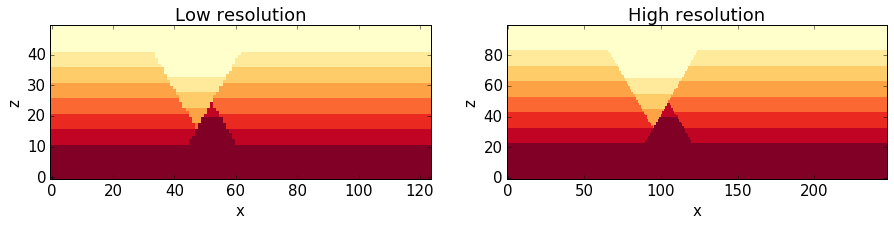
\includegraphics{2-Adjust-input_20_0.png}

Note: the following two subsections contain some slighly advanced
examples on how to use the possibility to adjust cell sizes through
scripts directly to autmote processes that are infeasible using the GUI
version of Noddy - as a `peek preview' of the automation for uncertainty
estimation that follows in a later section. Feel free to skip those two
sections if you are only interested in the basic features so far.


\section{Estimating computation time for a high-resolution model}
\label{notebooks/2-Adjust-input:estimating-computation-time-for-a-high-resolution-model}
You surely realised (if you ran these examples in an actual interactive
ipython notebook) that the computation of the high-resolution model
takes siginificantly longer than the low-resolution model. In a
practical case, this can be very important.

\begin{Verbatim}[commandchars=\\\{\}]
\PYG{c}{\PYGZsh{} We use here simply the time() function to evaulate the simualtion time.}
\PYG{c}{\PYGZsh{} This is not the best possible way to do it, but probably the simplest.}
\PYG{k+kn}{import} \PYG{n+nn}{time}
\PYG{n}{start\PYGZus{}time} \PYG{o}{=} \PYG{n}{time}\PYG{o}{.}\PYG{n}{time}\PYG{p}{(}\PYG{p}{)}
\PYG{n}{pynoddy}\PYG{o}{.}\PYG{n}{compute\PYGZus{}model}\PYG{p}{(}\PYG{n}{history}\PYG{p}{,} \PYG{n}{output\PYGZus{}name}\PYG{p}{)}
\PYG{n}{end\PYGZus{}time} \PYG{o}{=} \PYG{n}{time}\PYG{o}{.}\PYG{n}{time}\PYG{p}{(}\PYG{p}{)}

\PYG{k}{print}\PYG{p}{(}\PYG{l+s}{\PYGZdq{}}\PYG{l+s}{Simulation time for low\PYGZhy{}resolution model: }\PYG{l+s+si}{\PYGZpc{}5.2f}\PYG{l+s}{ seconds}\PYG{l+s}{\PYGZdq{}} \PYG{o}{\PYGZpc{}} \PYG{p}{(}\PYG{n}{end\PYGZus{}time} \PYG{o}{\PYGZhy{}} \PYG{n}{start\PYGZus{}time}\PYG{p}{)}\PYG{p}{)}

\PYG{n}{start\PYGZus{}time} \PYG{o}{=} \PYG{n}{time}\PYG{o}{.}\PYG{n}{time}\PYG{p}{(}\PYG{p}{)}
\PYG{n}{pynoddy}\PYG{o}{.}\PYG{n}{compute\PYGZus{}model}\PYG{p}{(}\PYG{n}{new\PYGZus{}history}\PYG{p}{,} \PYG{n}{new\PYGZus{}output\PYGZus{}name}\PYG{p}{)}
\PYG{n}{end\PYGZus{}time} \PYG{o}{=} \PYG{n}{time}\PYG{o}{.}\PYG{n}{time}\PYG{p}{(}\PYG{p}{)}

\PYG{k}{print}\PYG{p}{(}\PYG{l+s}{\PYGZdq{}}\PYG{l+s}{Simulation time for high\PYGZhy{}resolution model: }\PYG{l+s+si}{\PYGZpc{}5.2f}\PYG{l+s}{ seconds}\PYG{l+s}{\PYGZdq{}} \PYG{o}{\PYGZpc{}} \PYG{p}{(}\PYG{n}{end\PYGZus{}time} \PYG{o}{\PYGZhy{}} \PYG{n}{start\PYGZus{}time}\PYG{p}{)}\PYG{p}{)}
\end{Verbatim}

\begin{Verbatim}[commandchars=\\\{\}]
Simulation time for low\PYGZhy{}resolution model:  0.73 seconds
Simulation time for high\PYGZhy{}resolution model:  5.78 seconds
\end{Verbatim}

For an estimation of required computing time for a given discretisation,
let's evaulate the time for a couple of steps, plot, and extrapolate:

\begin{Verbatim}[commandchars=\\\{\}]
\PYG{c}{\PYGZsh{} perform computation for a range of cube sizes}
\PYG{n}{cube\PYGZus{}sizes} \PYG{o}{=} \PYG{n}{np}\PYG{o}{.}\PYG{n}{arange}\PYG{p}{(}\PYG{l+m+mi}{200}\PYG{p}{,}\PYG{l+m+mi}{49}\PYG{p}{,}\PYG{o}{\PYGZhy{}}\PYG{l+m+mi}{5}\PYG{p}{)}
\PYG{n}{times} \PYG{o}{=} \PYG{p}{[}\PYG{p}{]}
\PYG{n}{NH1} \PYG{o}{=} \PYG{n}{pynoddy}\PYG{o}{.}\PYG{n}{history}\PYG{o}{.}\PYG{n}{NoddyHistory}\PYG{p}{(}\PYG{n}{history}\PYG{p}{)}
\PYG{n}{tmp\PYGZus{}history} \PYG{o}{=} \PYG{l+s}{\PYGZdq{}}\PYG{l+s}{tmp\PYGZus{}history}\PYG{l+s}{\PYGZdq{}}
\PYG{n}{tmp\PYGZus{}output} \PYG{o}{=} \PYG{l+s}{\PYGZdq{}}\PYG{l+s}{tmp\PYGZus{}output}\PYG{l+s}{\PYGZdq{}}
\PYG{k}{for} \PYG{n}{cube\PYGZus{}size} \PYG{o+ow}{in} \PYG{n}{cube\PYGZus{}sizes}\PYG{p}{:}
    \PYG{n}{NH1}\PYG{o}{.}\PYG{n}{change\PYGZus{}cube\PYGZus{}size}\PYG{p}{(}\PYG{n}{cube\PYGZus{}size}\PYG{p}{)}
    \PYG{n}{NH1}\PYG{o}{.}\PYG{n}{write\PYGZus{}history}\PYG{p}{(}\PYG{n}{tmp\PYGZus{}history}\PYG{p}{)}
    \PYG{n}{start\PYGZus{}time} \PYG{o}{=} \PYG{n}{time}\PYG{o}{.}\PYG{n}{time}\PYG{p}{(}\PYG{p}{)}
    \PYG{n}{pynoddy}\PYG{o}{.}\PYG{n}{compute\PYGZus{}model}\PYG{p}{(}\PYG{n}{tmp\PYGZus{}history}\PYG{p}{,} \PYG{n}{tmp\PYGZus{}output}\PYG{p}{)}
    \PYG{n}{end\PYGZus{}time} \PYG{o}{=} \PYG{n}{time}\PYG{o}{.}\PYG{n}{time}\PYG{p}{(}\PYG{p}{)}
    \PYG{n}{times}\PYG{o}{.}\PYG{n}{append}\PYG{p}{(}\PYG{n}{end\PYGZus{}time} \PYG{o}{\PYGZhy{}} \PYG{n}{start\PYGZus{}time}\PYG{p}{)}
\PYG{n}{times} \PYG{o}{=} \PYG{n}{np}\PYG{o}{.}\PYG{n}{array}\PYG{p}{(}\PYG{n}{times}\PYG{p}{)}
\end{Verbatim}

\begin{Verbatim}[commandchars=\\\{\}]
\PYG{c}{\PYGZsh{} create plot}
\PYG{n}{fig} \PYG{o}{=} \PYG{n}{plt}\PYG{o}{.}\PYG{n}{figure}\PYG{p}{(}\PYG{n}{figsize}\PYG{o}{=}\PYG{p}{(}\PYG{l+m+mi}{18}\PYG{p}{,}\PYG{l+m+mi}{4}\PYG{p}{)}\PYG{p}{)}
\PYG{n}{ax1} \PYG{o}{=} \PYG{n}{fig}\PYG{o}{.}\PYG{n}{add\PYGZus{}subplot}\PYG{p}{(}\PYG{l+m+mi}{131}\PYG{p}{)}
\PYG{n}{ax2} \PYG{o}{=} \PYG{n}{fig}\PYG{o}{.}\PYG{n}{add\PYGZus{}subplot}\PYG{p}{(}\PYG{l+m+mi}{132}\PYG{p}{)}
\PYG{n}{ax3} \PYG{o}{=} \PYG{n}{fig}\PYG{o}{.}\PYG{n}{add\PYGZus{}subplot}\PYG{p}{(}\PYG{l+m+mi}{133}\PYG{p}{)}

\PYG{n}{ax1}\PYG{o}{.}\PYG{n}{plot}\PYG{p}{(}\PYG{n}{cube\PYGZus{}sizes}\PYG{p}{,} \PYG{n}{np}\PYG{o}{.}\PYG{n}{array}\PYG{p}{(}\PYG{n}{times}\PYG{p}{)}\PYG{p}{,} \PYG{l+s}{\PYGZsq{}}\PYG{l+s}{ro\PYGZhy{}}\PYG{l+s}{\PYGZsq{}}\PYG{p}{)}
\PYG{n}{ax1}\PYG{o}{.}\PYG{n}{set\PYGZus{}xlabel}\PYG{p}{(}\PYG{l+s}{\PYGZsq{}}\PYG{l+s}{cubesize [m]}\PYG{l+s}{\PYGZsq{}}\PYG{p}{)}
\PYG{n}{ax1}\PYG{o}{.}\PYG{n}{set\PYGZus{}ylabel}\PYG{p}{(}\PYG{l+s}{\PYGZsq{}}\PYG{l+s}{time [s]}\PYG{l+s}{\PYGZsq{}}\PYG{p}{)}
\PYG{n}{ax1}\PYG{o}{.}\PYG{n}{set\PYGZus{}title}\PYG{p}{(}\PYG{l+s}{\PYGZsq{}}\PYG{l+s}{Computation time}\PYG{l+s}{\PYGZsq{}}\PYG{p}{)}
\PYG{n}{ax1}\PYG{o}{.}\PYG{n}{set\PYGZus{}xlim}\PYG{p}{(}\PYG{n}{ax1}\PYG{o}{.}\PYG{n}{get\PYGZus{}xlim}\PYG{p}{(}\PYG{p}{)}\PYG{p}{[}\PYG{p}{:}\PYG{p}{:}\PYG{o}{\PYGZhy{}}\PYG{l+m+mi}{1}\PYG{p}{]}\PYG{p}{)}

\PYG{n}{ax2}\PYG{o}{.}\PYG{n}{plot}\PYG{p}{(}\PYG{n}{cube\PYGZus{}sizes}\PYG{p}{,} \PYG{n}{times}\PYG{o}{*}\PYG{o}{*}\PYG{p}{(}\PYG{l+m+mi}{1}\PYG{o}{/}\PYG{l+m+mf}{3.}\PYG{p}{)}\PYG{p}{,} \PYG{l+s}{\PYGZsq{}}\PYG{l+s}{bo\PYGZhy{}}\PYG{l+s}{\PYGZsq{}}\PYG{p}{)}
\PYG{n}{ax2}\PYG{o}{.}\PYG{n}{set\PYGZus{}xlabel}\PYG{p}{(}\PYG{l+s}{\PYGZsq{}}\PYG{l+s}{cubesize [m]}\PYG{l+s}{\PYGZsq{}}\PYG{p}{)}
\PYG{n}{ax2}\PYG{o}{.}\PYG{n}{set\PYGZus{}ylabel}\PYG{p}{(}\PYG{l+s}{\PYGZsq{}}\PYG{l+s}{(time [s])**(1/3)}\PYG{l+s}{\PYGZsq{}}\PYG{p}{)}
\PYG{n}{ax2}\PYG{o}{.}\PYG{n}{set\PYGZus{}title}\PYG{p}{(}\PYG{l+s}{\PYGZsq{}}\PYG{l+s}{Computation time (cuberoot)}\PYG{l+s}{\PYGZsq{}}\PYG{p}{)}
\PYG{n}{ax2}\PYG{o}{.}\PYG{n}{set\PYGZus{}xlim}\PYG{p}{(}\PYG{n}{ax2}\PYG{o}{.}\PYG{n}{get\PYGZus{}xlim}\PYG{p}{(}\PYG{p}{)}\PYG{p}{[}\PYG{p}{:}\PYG{p}{:}\PYG{o}{\PYGZhy{}}\PYG{l+m+mi}{1}\PYG{p}{]}\PYG{p}{)}

\PYG{n}{ax3}\PYG{o}{.}\PYG{n}{semilogy}\PYG{p}{(}\PYG{n}{cube\PYGZus{}sizes}\PYG{p}{,} \PYG{n}{times}\PYG{p}{,} \PYG{l+s}{\PYGZsq{}}\PYG{l+s}{go\PYGZhy{}}\PYG{l+s}{\PYGZsq{}}\PYG{p}{)}
\PYG{n}{ax3}\PYG{o}{.}\PYG{n}{set\PYGZus{}xlabel}\PYG{p}{(}\PYG{l+s}{\PYGZsq{}}\PYG{l+s}{cubesize [m]}\PYG{l+s}{\PYGZsq{}}\PYG{p}{)}
\PYG{n}{ax3}\PYG{o}{.}\PYG{n}{set\PYGZus{}ylabel}\PYG{p}{(}\PYG{l+s}{\PYGZsq{}}\PYG{l+s}{time [s]}\PYG{l+s}{\PYGZsq{}}\PYG{p}{)}
\PYG{n}{ax3}\PYG{o}{.}\PYG{n}{set\PYGZus{}title}\PYG{p}{(}\PYG{l+s}{\PYGZsq{}}\PYG{l+s}{Computation time (y\PYGZhy{}log)}\PYG{l+s}{\PYGZsq{}}\PYG{p}{)}
\PYG{n}{ax3}\PYG{o}{.}\PYG{n}{set\PYGZus{}xlim}\PYG{p}{(}\PYG{n}{ax3}\PYG{o}{.}\PYG{n}{get\PYGZus{}xlim}\PYG{p}{(}\PYG{p}{)}\PYG{p}{[}\PYG{p}{:}\PYG{p}{:}\PYG{o}{\PYGZhy{}}\PYG{l+m+mi}{1}\PYG{p}{]}\PYG{p}{)}
\end{Verbatim}

\begin{Verbatim}[commandchars=\\\{\}]
\PYG{p}{(}\PYG{l+m+mf}{200.0}\PYG{p}{,} \PYG{l+m+mf}{40.0}\PYG{p}{)}
\end{Verbatim}

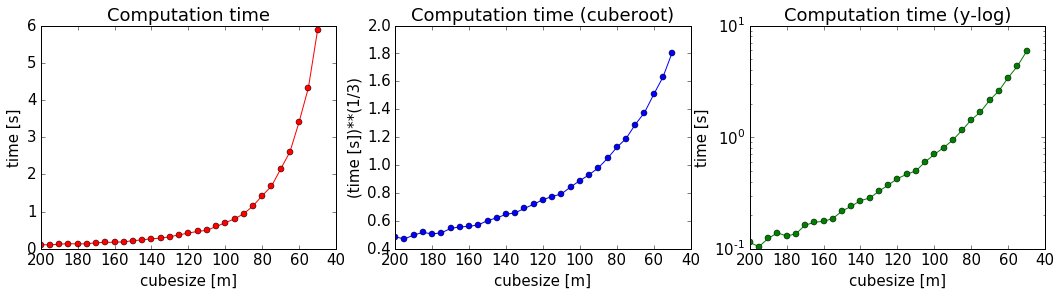
\includegraphics{2-Adjust-input_26_1.png}

It is actually quite interesting that the computation time does not
scale with cubesize to the power of three (as could be expected, given
that we have a mesh in three dimensions). Or am I missing something?

Anyway, just because we can: let's assume that the scaling is somehow
exponential and try to fit a model for a time prediction. Given the last
plot, it looks like we could fit a logarithmic model with probably an
additional exponent (as the line is obviously not straight), so
something like:
\begin{gather}
\begin{split}f(x) = a + \left( b \log_{10}(x) \right)^{-c}\end{split}\notag
\end{gather}
Let's try to fit the curve with \code{scipy.optimize.curve\_fit}:

\begin{Verbatim}[commandchars=\\\{\}]
\PYG{c}{\PYGZsh{} perform curve fitting with scipy.optimize}
\PYG{k+kn}{import} \PYG{n+nn}{scipy.optimize}
\PYG{c}{\PYGZsh{} define function to be fit}
\PYG{k}{def} \PYG{n+nf}{func}\PYG{p}{(}\PYG{n}{x}\PYG{p}{,}\PYG{n}{a}\PYG{p}{,}\PYG{n}{b}\PYG{p}{,}\PYG{n}{c}\PYG{p}{)}\PYG{p}{:}
    \PYG{k}{return} \PYG{n}{a} \PYG{o}{+} \PYG{p}{(}\PYG{n}{b}\PYG{o}{*}\PYG{n}{np}\PYG{o}{.}\PYG{n}{log10}\PYG{p}{(}\PYG{n}{x}\PYG{p}{)}\PYG{p}{)}\PYG{o}{*}\PYG{o}{*}\PYG{p}{(}\PYG{o}{\PYGZhy{}}\PYG{n}{c}\PYG{p}{)}

\PYG{n}{popt}\PYG{p}{,} \PYG{n}{pcov} \PYG{o}{=} \PYG{n}{scipy}\PYG{o}{.}\PYG{n}{optimize}\PYG{o}{.}\PYG{n}{curve\PYGZus{}fit}\PYG{p}{(}\PYG{n}{func}\PYG{p}{,} \PYG{n}{cube\PYGZus{}sizes}\PYG{p}{,} \PYG{n}{np}\PYG{o}{.}\PYG{n}{array}\PYG{p}{(}\PYG{n}{times}\PYG{p}{)}\PYG{p}{,} \PYG{n}{p0} \PYG{o}{=} \PYG{p}{[}\PYG{o}{\PYGZhy{}}\PYG{l+m+mi}{1}\PYG{p}{,} \PYG{l+m+mf}{0.5}\PYG{p}{,} \PYG{l+m+mi}{2}\PYG{p}{]}\PYG{p}{)}
\PYG{n}{popt}
\end{Verbatim}

\begin{Verbatim}[commandchars=\\\{\}]
\PYG{n}{array}\PYG{p}{(}\PYG{p}{[} \PYG{o}{\PYGZhy{}}\PYG{l+m+mf}{0.05618538}\PYG{p}{,}   \PYG{l+m+mf}{0.50990774}\PYG{p}{,}  \PYG{l+m+mf}{12.45183398}\PYG{p}{]}\PYG{p}{)}
\end{Verbatim}

Interesting, it looks like Noody scales with something like:
\begin{gather}
\begin{split}f(x) = \left( 0.5 \log_{10}(x) \right)^{-12}\end{split}\notag
\end{gather}
\textbf{Note}: if you understand more about computational complexity than me,
it might not be that interesting to you at all - if this is the case,
please contact me and tell me why this result could be expected...

\begin{Verbatim}[commandchars=\\\{\}]
\PYG{n}{a}\PYG{p}{,}\PYG{n}{b}\PYG{p}{,}\PYG{n}{c} \PYG{o}{=} \PYG{n}{popt}
\PYG{n}{cube\PYGZus{}range} \PYG{o}{=} \PYG{n}{np}\PYG{o}{.}\PYG{n}{arange}\PYG{p}{(}\PYG{l+m+mi}{200}\PYG{p}{,}\PYG{l+m+mi}{20}\PYG{p}{,}\PYG{o}{\PYGZhy{}}\PYG{l+m+mi}{1}\PYG{p}{)}
\PYG{n}{times\PYGZus{}eval} \PYG{o}{=} \PYG{n}{func}\PYG{p}{(}\PYG{n}{cube\PYGZus{}range}\PYG{p}{,} \PYG{n}{a}\PYG{p}{,} \PYG{n}{b}\PYG{p}{,} \PYG{n}{c}\PYG{p}{)}
\PYG{n}{fig} \PYG{o}{=} \PYG{n}{plt}\PYG{o}{.}\PYG{n}{figure}\PYG{p}{(}\PYG{p}{)}
\PYG{n}{ax} \PYG{o}{=} \PYG{n}{fig}\PYG{o}{.}\PYG{n}{add\PYGZus{}subplot}\PYG{p}{(}\PYG{l+m+mi}{111}\PYG{p}{)}
\PYG{n}{ax}\PYG{o}{.}\PYG{n}{semilogy}\PYG{p}{(}\PYG{n}{cube\PYGZus{}range}\PYG{p}{,} \PYG{n}{times\PYGZus{}eval}\PYG{p}{,} \PYG{l+s}{\PYGZsq{}}\PYG{l+s}{\PYGZhy{}}\PYG{l+s}{\PYGZsq{}}\PYG{p}{)}
\PYG{n}{ax}\PYG{o}{.}\PYG{n}{semilogy}\PYG{p}{(}\PYG{n}{cube\PYGZus{}sizes}\PYG{p}{,} \PYG{n}{times}\PYG{p}{,} \PYG{l+s}{\PYGZsq{}}\PYG{l+s}{ko}\PYG{l+s}{\PYGZsq{}}\PYG{p}{)}
\PYG{c}{\PYGZsh{} reverse x\PYGZhy{}axis}
\PYG{n}{ax}\PYG{o}{.}\PYG{n}{set\PYGZus{}xlim}\PYG{p}{(}\PYG{n}{ax}\PYG{o}{.}\PYG{n}{get\PYGZus{}xlim}\PYG{p}{(}\PYG{p}{)}\PYG{p}{[}\PYG{p}{:}\PYG{p}{:}\PYG{o}{\PYGZhy{}}\PYG{l+m+mi}{1}\PYG{p}{]}\PYG{p}{)}
\end{Verbatim}

\begin{Verbatim}[commandchars=\\\{\}]
\PYG{p}{(}\PYG{l+m+mf}{200.0}\PYG{p}{,} \PYG{l+m+mf}{20.0}\PYG{p}{)}
\end{Verbatim}

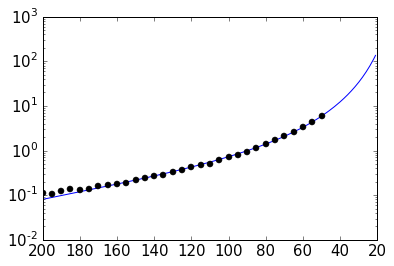
\includegraphics{2-Adjust-input_30_1.png}

Not too bad... let's evaluate the time for a cube size of 40 m:

\begin{Verbatim}[commandchars=\\\{\}]
\PYG{n}{cube\PYGZus{}size} \PYG{o}{=} \PYG{l+m+mi}{40} \PYG{c}{\PYGZsh{} m}
\PYG{n}{time\PYGZus{}est} \PYG{o}{=} \PYG{n}{func}\PYG{p}{(}\PYG{n}{cube\PYGZus{}size}\PYG{p}{,} \PYG{n}{a}\PYG{p}{,} \PYG{n}{b}\PYG{p}{,} \PYG{n}{c}\PYG{p}{)}
\PYG{k}{print}\PYG{p}{(}\PYG{l+s}{\PYGZdq{}}\PYG{l+s}{Estimated time for a cube size of }\PYG{l+s+si}{\PYGZpc{}d}\PYG{l+s}{ m: }\PYG{l+s+si}{\PYGZpc{}.1f}\PYG{l+s}{ seconds}\PYG{l+s}{\PYGZdq{}} \PYG{o}{\PYGZpc{}} \PYG{p}{(}\PYG{n}{cube\PYGZus{}size}\PYG{p}{,} \PYG{n}{time\PYGZus{}est}\PYG{p}{)}\PYG{p}{)}
\end{Verbatim}

\begin{Verbatim}[commandchars=\\\{\}]
Estimated time for a cube size of 40 m: 12.4 seconds
\end{Verbatim}

Now let's check the actual simulation time:

\begin{Verbatim}[commandchars=\\\{\}]
\PYG{n}{NH1}\PYG{o}{.}\PYG{n}{change\PYGZus{}cube\PYGZus{}size}\PYG{p}{(}\PYG{n}{cube\PYGZus{}size}\PYG{p}{)}
\PYG{n}{NH1}\PYG{o}{.}\PYG{n}{write\PYGZus{}history}\PYG{p}{(}\PYG{n}{tmp\PYGZus{}history}\PYG{p}{)}
\PYG{n}{start\PYGZus{}time} \PYG{o}{=} \PYG{n}{time}\PYG{o}{.}\PYG{n}{time}\PYG{p}{(}\PYG{p}{)}
\PYG{n}{pynoddy}\PYG{o}{.}\PYG{n}{compute\PYGZus{}model}\PYG{p}{(}\PYG{n}{tmp\PYGZus{}history}\PYG{p}{,} \PYG{n}{tmp\PYGZus{}output}\PYG{p}{)}
\PYG{n}{end\PYGZus{}time} \PYG{o}{=} \PYG{n}{time}\PYG{o}{.}\PYG{n}{time}\PYG{p}{(}\PYG{p}{)}
\PYG{n}{time\PYGZus{}comp} \PYG{o}{=} \PYG{n}{end\PYGZus{}time} \PYG{o}{\PYGZhy{}} \PYG{n}{start\PYGZus{}time}

\PYG{k}{print}\PYG{p}{(}\PYG{l+s}{\PYGZdq{}}\PYG{l+s}{Actual computation time for a cube size of }\PYG{l+s+si}{\PYGZpc{}d}\PYG{l+s}{ m: }\PYG{l+s+si}{\PYGZpc{}.1f}\PYG{l+s}{ seconds}\PYG{l+s}{\PYGZdq{}} \PYG{o}{\PYGZpc{}} \PYG{p}{(}\PYG{n}{cube\PYGZus{}size}\PYG{p}{,} \PYG{n}{time\PYGZus{}comp}\PYG{p}{)}\PYG{p}{)}
\end{Verbatim}

\begin{Verbatim}[commandchars=\\\{\}]
Actual computation time for a cube size of 40 m: 11.6 seconds
\end{Verbatim}

Not too bad, probably in the range of the inherent variability... and if
we check it in the plot:

\begin{Verbatim}[commandchars=\\\{\}]
\PYG{n}{fig} \PYG{o}{=} \PYG{n}{plt}\PYG{o}{.}\PYG{n}{figure}\PYG{p}{(}\PYG{p}{)}
\PYG{n}{ax} \PYG{o}{=} \PYG{n}{fig}\PYG{o}{.}\PYG{n}{add\PYGZus{}subplot}\PYG{p}{(}\PYG{l+m+mi}{111}\PYG{p}{)}
\PYG{n}{ax}\PYG{o}{.}\PYG{n}{semilogy}\PYG{p}{(}\PYG{n}{cube\PYGZus{}range}\PYG{p}{,} \PYG{n}{times\PYGZus{}eval}\PYG{p}{,} \PYG{l+s}{\PYGZsq{}}\PYG{l+s}{\PYGZhy{}}\PYG{l+s}{\PYGZsq{}}\PYG{p}{)}
\PYG{n}{ax}\PYG{o}{.}\PYG{n}{semilogy}\PYG{p}{(}\PYG{n}{cube\PYGZus{}sizes}\PYG{p}{,} \PYG{n}{times}\PYG{p}{,} \PYG{l+s}{\PYGZsq{}}\PYG{l+s}{ko}\PYG{l+s}{\PYGZsq{}}\PYG{p}{)}
\PYG{n}{ax}\PYG{o}{.}\PYG{n}{semilogy}\PYG{p}{(}\PYG{n}{cube\PYGZus{}size}\PYG{p}{,} \PYG{n}{time\PYGZus{}comp}\PYG{p}{,} \PYG{l+s}{\PYGZsq{}}\PYG{l+s}{ro}\PYG{l+s}{\PYGZsq{}}\PYG{p}{)}
\PYG{c}{\PYGZsh{} reverse x\PYGZhy{}axis}
\PYG{n}{ax}\PYG{o}{.}\PYG{n}{set\PYGZus{}xlim}\PYG{p}{(}\PYG{n}{ax}\PYG{o}{.}\PYG{n}{get\PYGZus{}xlim}\PYG{p}{(}\PYG{p}{)}\PYG{p}{[}\PYG{p}{:}\PYG{p}{:}\PYG{o}{\PYGZhy{}}\PYG{l+m+mi}{1}\PYG{p}{]}\PYG{p}{)}
\end{Verbatim}

\begin{Verbatim}[commandchars=\\\{\}]
\PYG{p}{(}\PYG{l+m+mf}{200.0}\PYG{p}{,} \PYG{l+m+mf}{20.0}\PYG{p}{)}
\end{Verbatim}

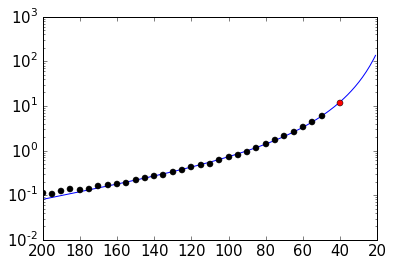
\includegraphics{2-Adjust-input_36_1.png}

Anyway, the point of this excercise was not a precise evaluation of
Noddy's computational complexity, but to provide a simple means of
evaluating computation time for a high resolution model, using the
flexibility of writing simple scripts using pynoddy, and a couple of
additional python modules.

For a realistic case, it should, of course, be sufficient to determine
the time based on a lot less computed points. If you like, test it with
your favourite model and tell me if it proved useful (or not)!


\section{Simple convergence study}
\label{notebooks/2-Adjust-input:simple-convergence-study}
So: why would we want to run a high-resolution model, anyway? Well, of
course, it produces nicer pictures - but on a scientific level, that's
completely irrelevant (haha, not true - so nice if it would be...).

Anyway, if we want to use the model in a scientific study, for example
to evaluate volume of specific units, or to estimate the geological
topology (Mark is working on this topic with some cool ideas - example
to be implemented here, ``soon''), we want to know if the resolution of
the model is actually high enough to produce meaningful results.

As a simple example of the evaluation of model resolution, we will here
inlcude a volume convergence study, i.e. we will estimate at which level
of increasing model resolution the estimated block volumes do not change
anymore.

The entire procedure is very similar to the computational time
evaluation above, only that we now also analyse the output and determine
the rock volumes of each defined geological unit:

\begin{Verbatim}[commandchars=\\\{\}]
\PYG{c}{\PYGZsh{} perform computation for a range of cube sizes}
\PYG{n+nb}{reload}\PYG{p}{(}\PYG{n}{pynoddy}\PYG{o}{.}\PYG{n}{output}\PYG{p}{)}
\PYG{n}{cube\PYGZus{}sizes} \PYG{o}{=} \PYG{n}{np}\PYG{o}{.}\PYG{n}{arange}\PYG{p}{(}\PYG{l+m+mi}{200}\PYG{p}{,}\PYG{l+m+mi}{49}\PYG{p}{,}\PYG{o}{\PYGZhy{}}\PYG{l+m+mi}{5}\PYG{p}{)}
\PYG{n}{all\PYGZus{}volumes} \PYG{o}{=} \PYG{p}{[}\PYG{p}{]}
\PYG{n}{N\PYGZus{}tmp} \PYG{o}{=} \PYG{n}{pynoddy}\PYG{o}{.}\PYG{n}{history}\PYG{o}{.}\PYG{n}{NoddyHistory}\PYG{p}{(}\PYG{n}{history}\PYG{p}{)}
\PYG{n}{tmp\PYGZus{}history} \PYG{o}{=} \PYG{l+s}{\PYGZdq{}}\PYG{l+s}{tmp\PYGZus{}history}\PYG{l+s}{\PYGZdq{}}
\PYG{n}{tmp\PYGZus{}output} \PYG{o}{=} \PYG{l+s}{\PYGZdq{}}\PYG{l+s}{tmp\PYGZus{}output}\PYG{l+s}{\PYGZdq{}}
\PYG{k}{for} \PYG{n}{cube\PYGZus{}size} \PYG{o+ow}{in} \PYG{n}{cube\PYGZus{}sizes}\PYG{p}{:}
    \PYG{c}{\PYGZsh{} adjust cube size}
    \PYG{n}{N\PYGZus{}tmp}\PYG{o}{.}\PYG{n}{change\PYGZus{}cube\PYGZus{}size}\PYG{p}{(}\PYG{n}{cube\PYGZus{}size}\PYG{p}{)}
    \PYG{n}{N\PYGZus{}tmp}\PYG{o}{.}\PYG{n}{write\PYGZus{}history}\PYG{p}{(}\PYG{n}{tmp\PYGZus{}history}\PYG{p}{)}
    \PYG{n}{pynoddy}\PYG{o}{.}\PYG{n}{compute\PYGZus{}model}\PYG{p}{(}\PYG{n}{tmp\PYGZus{}history}\PYG{p}{,} \PYG{n}{tmp\PYGZus{}output}\PYG{p}{)}
    \PYG{c}{\PYGZsh{} open simulated model and determine volumes}
    \PYG{n}{O\PYGZus{}tmp} \PYG{o}{=} \PYG{n}{pynoddy}\PYG{o}{.}\PYG{n}{output}\PYG{o}{.}\PYG{n}{NoddyOutput}\PYG{p}{(}\PYG{n}{tmp\PYGZus{}output}\PYG{p}{)}
    \PYG{n}{O\PYGZus{}tmp}\PYG{o}{.}\PYG{n}{determine\PYGZus{}unit\PYGZus{}volumes}\PYG{p}{(}\PYG{p}{)}
    \PYG{n}{all\PYGZus{}volumes}\PYG{o}{.}\PYG{n}{append}\PYG{p}{(}\PYG{n}{O\PYGZus{}tmp}\PYG{o}{.}\PYG{n}{unit\PYGZus{}volumes}\PYG{p}{)}
\end{Verbatim}

\begin{Verbatim}[commandchars=\\\{\}]
\PYG{n}{all\PYGZus{}volumes} \PYG{o}{=} \PYG{n}{np}\PYG{o}{.}\PYG{n}{array}\PYG{p}{(}\PYG{n}{all\PYGZus{}volumes}\PYG{p}{)}
\PYG{n}{fig} \PYG{o}{=} \PYG{n}{plt}\PYG{o}{.}\PYG{n}{figure}\PYG{p}{(}\PYG{n}{figsize}\PYG{o}{=}\PYG{p}{(}\PYG{l+m+mi}{16}\PYG{p}{,}\PYG{l+m+mi}{4}\PYG{p}{)}\PYG{p}{)}
\PYG{n}{ax1} \PYG{o}{=} \PYG{n}{fig}\PYG{o}{.}\PYG{n}{add\PYGZus{}subplot}\PYG{p}{(}\PYG{l+m+mi}{121}\PYG{p}{)}
\PYG{n}{ax2} \PYG{o}{=} \PYG{n}{fig}\PYG{o}{.}\PYG{n}{add\PYGZus{}subplot}\PYG{p}{(}\PYG{l+m+mi}{122}\PYG{p}{)}

\PYG{c}{\PYGZsh{} separate into two plots for better visibility:}
\PYG{k}{for} \PYG{n}{i} \PYG{o+ow}{in} \PYG{n+nb}{range}\PYG{p}{(}\PYG{n}{np}\PYG{o}{.}\PYG{n}{shape}\PYG{p}{(}\PYG{n}{all\PYGZus{}volumes}\PYG{p}{)}\PYG{p}{[}\PYG{l+m+mi}{1}\PYG{p}{]}\PYG{p}{)}\PYG{p}{:}
    \PYG{k}{if} \PYG{n}{i} \PYG{o}{\PYGZlt{}} \PYG{l+m+mi}{4}\PYG{p}{:}
        \PYG{n}{ax1}\PYG{o}{.}\PYG{n}{plot}\PYG{p}{(}\PYG{n}{cube\PYGZus{}sizes}\PYG{p}{,} \PYG{n}{all\PYGZus{}volumes}\PYG{p}{[}\PYG{p}{:}\PYG{p}{,}\PYG{n}{i}\PYG{p}{]}\PYG{p}{,} \PYG{l+s}{\PYGZsq{}}\PYG{l+s}{o\PYGZhy{}}\PYG{l+s}{\PYGZsq{}}\PYG{p}{,} \PYG{n}{label}\PYG{o}{=}\PYG{l+s}{\PYGZsq{}}\PYG{l+s}{unit }\PYG{l+s+si}{\PYGZpc{}d}\PYG{l+s}{\PYGZsq{}} \PYG{o}{\PYGZpc{}}\PYG{n}{i}\PYG{p}{)}
    \PYG{k}{else}\PYG{p}{:}
        \PYG{n}{ax2}\PYG{o}{.}\PYG{n}{plot}\PYG{p}{(}\PYG{n}{cube\PYGZus{}sizes}\PYG{p}{,} \PYG{n}{all\PYGZus{}volumes}\PYG{p}{[}\PYG{p}{:}\PYG{p}{,}\PYG{n}{i}\PYG{p}{]}\PYG{p}{,} \PYG{l+s}{\PYGZsq{}}\PYG{l+s}{o\PYGZhy{}}\PYG{l+s}{\PYGZsq{}}\PYG{p}{,} \PYG{n}{label}\PYG{o}{=}\PYG{l+s}{\PYGZsq{}}\PYG{l+s}{unit }\PYG{l+s+si}{\PYGZpc{}d}\PYG{l+s}{\PYGZsq{}} \PYG{o}{\PYGZpc{}}\PYG{n}{i}\PYG{p}{)}

\PYG{n}{ax1}\PYG{o}{.}\PYG{n}{legend}\PYG{p}{(}\PYG{n}{loc}\PYG{o}{=}\PYG{l+m+mi}{2}\PYG{p}{)}
\PYG{n}{ax2}\PYG{o}{.}\PYG{n}{legend}\PYG{p}{(}\PYG{n}{loc}\PYG{o}{=}\PYG{l+m+mi}{2}\PYG{p}{)}
\PYG{c}{\PYGZsh{} reverse axes}
\PYG{n}{ax1}\PYG{o}{.}\PYG{n}{set\PYGZus{}xlim}\PYG{p}{(}\PYG{n}{ax1}\PYG{o}{.}\PYG{n}{get\PYGZus{}xlim}\PYG{p}{(}\PYG{p}{)}\PYG{p}{[}\PYG{p}{:}\PYG{p}{:}\PYG{o}{\PYGZhy{}}\PYG{l+m+mi}{1}\PYG{p}{]}\PYG{p}{)}
\PYG{n}{ax2}\PYG{o}{.}\PYG{n}{set\PYGZus{}xlim}\PYG{p}{(}\PYG{n}{ax2}\PYG{o}{.}\PYG{n}{get\PYGZus{}xlim}\PYG{p}{(}\PYG{p}{)}\PYG{p}{[}\PYG{p}{:}\PYG{p}{:}\PYG{o}{\PYGZhy{}}\PYG{l+m+mi}{1}\PYG{p}{]}\PYG{p}{)}

\PYG{n}{ax1}\PYG{o}{.}\PYG{n}{set\PYGZus{}xlabel}\PYG{p}{(}\PYG{l+s}{\PYGZdq{}}\PYG{l+s}{Block size [m]}\PYG{l+s}{\PYGZdq{}}\PYG{p}{)}
\PYG{n}{ax1}\PYG{o}{.}\PYG{n}{set\PYGZus{}ylabel}\PYG{p}{(}\PYG{l+s}{\PYGZdq{}}\PYG{l+s}{Total unit volume [m**3]}\PYG{l+s}{\PYGZdq{}}\PYG{p}{)}
\PYG{n}{ax2}\PYG{o}{.}\PYG{n}{set\PYGZus{}xlabel}\PYG{p}{(}\PYG{l+s}{\PYGZdq{}}\PYG{l+s}{Block size [m]}\PYG{l+s}{\PYGZdq{}}\PYG{p}{)}
\PYG{n}{ax2}\PYG{o}{.}\PYG{n}{set\PYGZus{}ylabel}\PYG{p}{(}\PYG{l+s}{\PYGZdq{}}\PYG{l+s}{Total unit volume [m**3]}\PYG{l+s}{\PYGZdq{}}\PYG{p}{)}
\end{Verbatim}

\begin{Verbatim}[commandchars=\\\{\}]
\PYGZlt{}matplotlib.text.Text at 0x107eb7250\PYGZgt{}
\end{Verbatim}

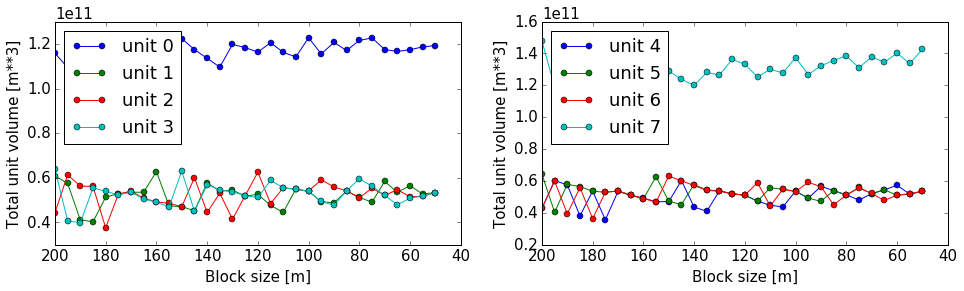
\includegraphics{2-Adjust-input_40_1.png}

It looks like the volumes would start to converge from about a block
size of 100 m. The example model is pretty small and simple, probably
not the best example for this study. Try it out with your own, highly
complex, favourite pet model :-)


\chapter{Geological events in pynoddy: organisation and adpatiation}
\label{notebooks/3-Events:geological-events-in-pynoddy-organisation-and-adpatiation}\label{notebooks/3-Events::doc}
We will here describe how the single geological events of a Noddy
history are organised within pynoddy. We will then evaluate in some more
detail how aspects of events can be adapted and their effect evaluated.

\begin{Verbatim}[commandchars=\\\{\}]
\PYG{k+kn}{from} \PYG{n+nn}{IPython.core.display} \PYG{k+kn}{import} \PYG{n}{HTML}
\PYG{n}{css\PYGZus{}file} \PYG{o}{=} \PYG{l+s}{\PYGZsq{}}\PYG{l+s}{pynoddy.css}\PYG{l+s}{\PYGZsq{}}
\PYG{n}{HTML}\PYG{p}{(}\PYG{n+nb}{open}\PYG{p}{(}\PYG{n}{css\PYGZus{}file}\PYG{p}{,} \PYG{l+s}{\PYGZdq{}}\PYG{l+s}{r}\PYG{l+s}{\PYGZdq{}}\PYG{p}{)}\PYG{o}{.}\PYG{n}{read}\PYG{p}{(}\PYG{p}{)}\PYG{p}{)}
\end{Verbatim}

\begin{Verbatim}[commandchars=\\\{\}]
\PYGZpc{}matplotlib inline
\end{Verbatim}


\section{Loading events from a Noddy history}
\label{notebooks/3-Events:loading-events-from-a-noddy-history}
In the current set-up of pynoddy, we always start with a pre-defined
Noddy history loaded from a file, and then change aspects of the history
and the single events. The first step is therefore to load the history
file and to extract the single geological events. This is done
automatically as default when loading the history file into the History
object:

\begin{Verbatim}[commandchars=\\\{\}]
\PYG{k+kn}{import} \PYG{n+nn}{sys}\PYG{o}{,} \PYG{n+nn}{os}
\PYG{k+kn}{import} \PYG{n+nn}{matplotlib.pyplot} \PYG{k+kn}{as} \PYG{n+nn}{plt}
\PYG{c}{\PYGZsh{} adjust some settings for matplotlib}
\PYG{k+kn}{from} \PYG{n+nn}{matplotlib} \PYG{k+kn}{import} \PYG{n}{rcParams}
\PYG{c}{\PYGZsh{} print rcParams}
\PYG{n}{rcParams}\PYG{p}{[}\PYG{l+s}{\PYGZsq{}}\PYG{l+s}{font.size}\PYG{l+s}{\PYGZsq{}}\PYG{p}{]} \PYG{o}{=} \PYG{l+m+mi}{15}
\PYG{c}{\PYGZsh{} determine path of repository to set paths corretly below}
\PYG{n}{repo\PYGZus{}path} \PYG{o}{=} \PYG{n}{os}\PYG{o}{.}\PYG{n}{path}\PYG{o}{.}\PYG{n}{realpath}\PYG{p}{(}\PYG{l+s}{\PYGZsq{}}\PYG{l+s}{../..}\PYG{l+s}{\PYGZsq{}}\PYG{p}{)}

\PYG{k+kn}{import} \PYG{n+nn}{pynoddy}
\PYG{k+kn}{import} \PYG{n+nn}{pynoddy.history}
\PYG{k+kn}{import} \PYG{n+nn}{pynoddy.events}
\PYG{k+kn}{import} \PYG{n+nn}{pynoddy.output}
\PYG{n+nb}{reload}\PYG{p}{(}\PYG{n}{pynoddy}\PYG{p}{)}
\end{Verbatim}

\begin{Verbatim}[commandchars=\\\{\}]
\PYGZlt{}module \PYGZsq{}pynoddy\PYGZsq{} from \PYGZsq{}/Users/flow/git/pynoddy/pynoddy/\PYGZus{}\PYGZus{}init\PYGZus{}\PYGZus{}.pyc\PYGZsq{}\PYGZgt{}
\end{Verbatim}

\begin{Verbatim}[commandchars=\\\{\}]
\PYG{c}{\PYGZsh{} Change to sandbox directory to store results}
\PYG{n}{os}\PYG{o}{.}\PYG{n}{chdir}\PYG{p}{(}\PYG{n}{os}\PYG{o}{.}\PYG{n}{path}\PYG{o}{.}\PYG{n}{join}\PYG{p}{(}\PYG{n}{repo\PYGZus{}path}\PYG{p}{,} \PYG{l+s}{\PYGZsq{}}\PYG{l+s}{sandbox}\PYG{l+s}{\PYGZsq{}}\PYG{p}{)}\PYG{p}{)}

\PYG{c}{\PYGZsh{} Path to exmaple directory in this repository}
\PYG{n}{example\PYGZus{}directory} \PYG{o}{=} \PYG{n}{os}\PYG{o}{.}\PYG{n}{path}\PYG{o}{.}\PYG{n}{join}\PYG{p}{(}\PYG{n}{repo\PYGZus{}path}\PYG{p}{,}\PYG{l+s}{\PYGZsq{}}\PYG{l+s}{examples}\PYG{l+s}{\PYGZsq{}}\PYG{p}{)}
\PYG{c}{\PYGZsh{} Compute noddy model for history file}
\PYG{n}{history} \PYG{o}{=} \PYG{l+s}{\PYGZsq{}}\PYG{l+s}{simple\PYGZus{}two\PYGZus{}faults.his}\PYG{l+s}{\PYGZsq{}}
\PYG{n}{history\PYGZus{}ori} \PYG{o}{=} \PYG{n}{os}\PYG{o}{.}\PYG{n}{path}\PYG{o}{.}\PYG{n}{join}\PYG{p}{(}\PYG{n}{example\PYGZus{}directory}\PYG{p}{,} \PYG{n}{history}\PYG{p}{)}
\PYG{n}{output\PYGZus{}name} \PYG{o}{=} \PYG{l+s}{\PYGZsq{}}\PYG{l+s}{noddy\PYGZus{}out}\PYG{l+s}{\PYGZsq{}}
\PYG{n+nb}{reload}\PYG{p}{(}\PYG{n}{pynoddy}\PYG{o}{.}\PYG{n}{history}\PYG{p}{)}
\PYG{n+nb}{reload}\PYG{p}{(}\PYG{n}{pynoddy}\PYG{o}{.}\PYG{n}{events}\PYG{p}{)}
\PYG{n}{H1} \PYG{o}{=} \PYG{n}{pynoddy}\PYG{o}{.}\PYG{n}{history}\PYG{o}{.}\PYG{n}{NoddyHistory}\PYG{p}{(}\PYG{n}{history\PYGZus{}ori}\PYG{p}{)}
\PYG{c}{\PYGZsh{} Before we do anything else, let\PYGZsq{}s actually define the cube size here to}
\PYG{c}{\PYGZsh{} adjust the resolution for all subsequent examples}
\PYG{n}{H1}\PYG{o}{.}\PYG{n}{change\PYGZus{}cube\PYGZus{}size}\PYG{p}{(}\PYG{l+m+mi}{100}\PYG{p}{)}
\PYG{c}{\PYGZsh{} compute model \PYGZhy{} note: not strictly required, here just to ensure changed cube size}
\PYG{n}{H1}\PYG{o}{.}\PYG{n}{write\PYGZus{}history}\PYG{p}{(}\PYG{n}{history}\PYG{p}{)}
\PYG{n}{pynoddy}\PYG{o}{.}\PYG{n}{compute\PYGZus{}model}\PYG{p}{(}\PYG{n}{history}\PYG{p}{,} \PYG{n}{output\PYGZus{}name}\PYG{p}{)}
\end{Verbatim}

\begin{Verbatim}[commandchars=\\\{\}]
\PYG{l+s}{\PYGZsq{}}\PYG{l+s}{\PYGZsq{}}
\end{Verbatim}

Events are stored in the object dictionary ``events'' (who would have
thought), where the key corresponds to the position in the timeline:

\begin{Verbatim}[commandchars=\\\{\}]
\PYG{n}{H1}\PYG{o}{.}\PYG{n}{events}
\end{Verbatim}

\begin{Verbatim}[commandchars=\\\{\}]
\PYGZob{}1: \PYGZlt{}pynoddy.events.Stratigraphy at 0x10cf2b410\PYGZgt{},
 2: \PYGZlt{}pynoddy.events.Fault at 0x10cf2b450\PYGZgt{},
 3: \PYGZlt{}pynoddy.events.Fault at 0x10cf2b490\PYGZgt{}\PYGZcb{}
\end{Verbatim}

We can see here that three events are defined in the history. Events are
organised as objects themselves, containing all the relevant properties
and information about the events. For example, the second fault event is
defined as:

\begin{Verbatim}[commandchars=\\\{\}]
\PYG{n}{H1}\PYG{o}{.}\PYG{n}{events}\PYG{p}{[}\PYG{l+m+mi}{3}\PYG{p}{]}\PYG{o}{.}\PYG{n}{properties}
\end{Verbatim}

\begin{Verbatim}[commandchars=\\\{\}]
\PYG{p}{\PYGZob{}}\PYG{l+s}{\PYGZsq{}}\PYG{l+s}{Amplitude}\PYG{l+s}{\PYGZsq{}}\PYG{p}{:} \PYG{l+m+mf}{2000.0}\PYG{p}{,}
 \PYG{l+s}{\PYGZsq{}}\PYG{l+s}{Blue}\PYG{l+s}{\PYGZsq{}}\PYG{p}{:} \PYG{l+m+mf}{0.0}\PYG{p}{,}
 \PYG{l+s}{\PYGZsq{}}\PYG{l+s}{Color Name}\PYG{l+s}{\PYGZsq{}}\PYG{p}{:} \PYG{l+s}{\PYGZsq{}}\PYG{l+s}{Custom Colour 5}\PYG{l+s}{\PYGZsq{}}\PYG{p}{,}
 \PYG{l+s}{\PYGZsq{}}\PYG{l+s}{Cyl Index}\PYG{l+s}{\PYGZsq{}}\PYG{p}{:} \PYG{l+m+mf}{0.0}\PYG{p}{,}
 \PYG{l+s}{\PYGZsq{}}\PYG{l+s}{Dip}\PYG{l+s}{\PYGZsq{}}\PYG{p}{:} \PYG{l+m+mf}{60.0}\PYG{p}{,}
 \PYG{l+s}{\PYGZsq{}}\PYG{l+s}{Dip Direction}\PYG{l+s}{\PYGZsq{}}\PYG{p}{:} \PYG{l+m+mf}{270.0}\PYG{p}{,}
 \PYG{l+s}{\PYGZsq{}}\PYG{l+s}{Geometry}\PYG{l+s}{\PYGZsq{}}\PYG{p}{:} \PYG{l+s}{\PYGZsq{}}\PYG{l+s}{Translation}\PYG{l+s}{\PYGZsq{}}\PYG{p}{,}
 \PYG{l+s}{\PYGZsq{}}\PYG{l+s}{Green}\PYG{l+s}{\PYGZsq{}}\PYG{p}{:} \PYG{l+m+mf}{0.0}\PYG{p}{,}
 \PYG{l+s}{\PYGZsq{}}\PYG{l+s}{Movement}\PYG{l+s}{\PYGZsq{}}\PYG{p}{:} \PYG{l+s}{\PYGZsq{}}\PYG{l+s}{Hanging Wall}\PYG{l+s}{\PYGZsq{}}\PYG{p}{,}
 \PYG{l+s}{\PYGZsq{}}\PYG{l+s}{Pitch}\PYG{l+s}{\PYGZsq{}}\PYG{p}{:} \PYG{l+m+mf}{90.0}\PYG{p}{,}
 \PYG{l+s}{\PYGZsq{}}\PYG{l+s}{Profile Pitch}\PYG{l+s}{\PYGZsq{}}\PYG{p}{:} \PYG{l+m+mf}{90.0}\PYG{p}{,}
 \PYG{l+s}{\PYGZsq{}}\PYG{l+s}{Radius}\PYG{l+s}{\PYGZsq{}}\PYG{p}{:} \PYG{l+m+mf}{1000.0}\PYG{p}{,}
 \PYG{l+s}{\PYGZsq{}}\PYG{l+s}{Red}\PYG{l+s}{\PYGZsq{}}\PYG{p}{:} \PYG{l+m+mf}{254.0}\PYG{p}{,}
 \PYG{l+s}{\PYGZsq{}}\PYG{l+s}{Rotation}\PYG{l+s}{\PYGZsq{}}\PYG{p}{:} \PYG{l+m+mf}{30.0}\PYG{p}{,}
 \PYG{l+s}{\PYGZsq{}}\PYG{l+s}{Slip}\PYG{l+s}{\PYGZsq{}}\PYG{p}{:} \PYG{l+m+mf}{1000.0}\PYG{p}{,}
 \PYG{l+s}{\PYGZsq{}}\PYG{l+s}{X}\PYG{l+s}{\PYGZsq{}}\PYG{p}{:} \PYG{l+m+mf}{5500.0}\PYG{p}{,}
 \PYG{l+s}{\PYGZsq{}}\PYG{l+s}{XAxis}\PYG{l+s}{\PYGZsq{}}\PYG{p}{:} \PYG{l+m+mf}{2000.0}\PYG{p}{,}
 \PYG{l+s}{\PYGZsq{}}\PYG{l+s}{Y}\PYG{l+s}{\PYGZsq{}}\PYG{p}{:} \PYG{l+m+mf}{7000.0}\PYG{p}{,}
 \PYG{l+s}{\PYGZsq{}}\PYG{l+s}{YAxis}\PYG{l+s}{\PYGZsq{}}\PYG{p}{:} \PYG{l+m+mf}{2000.0}\PYG{p}{,}
 \PYG{l+s}{\PYGZsq{}}\PYG{l+s}{Z}\PYG{l+s}{\PYGZsq{}}\PYG{p}{:} \PYG{l+m+mf}{5000.0}\PYG{p}{,}
 \PYG{l+s}{\PYGZsq{}}\PYG{l+s}{ZAxis}\PYG{l+s}{\PYGZsq{}}\PYG{p}{:} \PYG{l+m+mf}{2000.0}\PYG{p}{\PYGZcb{}}
\end{Verbatim}


\section{Changing aspects of geological events}
\label{notebooks/3-Events:changing-aspects-of-geological-events}
So what we now want to do, of course, is to change aspects of these
events and to evaluate the effect on the resulting geological model.
Parameters can directly be updated in the properties dictionary:

\begin{Verbatim}[commandchars=\\\{\}]
\PYG{n}{H1} \PYG{o}{=} \PYG{n}{pynoddy}\PYG{o}{.}\PYG{n}{history}\PYG{o}{.}\PYG{n}{NoddyHistory}\PYG{p}{(}\PYG{n}{history\PYGZus{}ori}\PYG{p}{)}
\PYG{c}{\PYGZsh{} get the original dip of the fault}
\PYG{n}{dip\PYGZus{}ori} \PYG{o}{=} \PYG{n}{H1}\PYG{o}{.}\PYG{n}{events}\PYG{p}{[}\PYG{l+m+mi}{3}\PYG{p}{]}\PYG{o}{.}\PYG{n}{properties}\PYG{p}{[}\PYG{l+s}{\PYGZsq{}}\PYG{l+s}{Dip}\PYG{l+s}{\PYGZsq{}}\PYG{p}{]}

\PYG{c}{\PYGZsh{} add 10 degrees to dip}
\PYG{n}{add\PYGZus{}dip} \PYG{o}{=} \PYG{o}{\PYGZhy{}}\PYG{l+m+mi}{10}
\PYG{n}{dip\PYGZus{}new} \PYG{o}{=} \PYG{n}{dip\PYGZus{}ori} \PYG{o}{+} \PYG{n}{add\PYGZus{}dip}

\PYG{c}{\PYGZsh{} and assign back to properties dictionary:}
\PYG{n}{H1}\PYG{o}{.}\PYG{n}{events}\PYG{p}{[}\PYG{l+m+mi}{3}\PYG{p}{]}\PYG{o}{.}\PYG{n}{properties}\PYG{p}{[}\PYG{l+s}{\PYGZsq{}}\PYG{l+s}{Dip}\PYG{l+s}{\PYGZsq{}}\PYG{p}{]} \PYG{o}{=} \PYG{n}{dip\PYGZus{}new}
\PYG{c}{\PYGZsh{} H1.events[2].properties[\PYGZsq{}Dip\PYGZsq{}] = dip\PYGZus{}new1}
\end{Verbatim}

\begin{Verbatim}[commandchars=\\\{\}]
\PYG{n}{new\PYGZus{}history} \PYG{o}{=} \PYG{l+s}{\PYGZdq{}}\PYG{l+s}{dip\PYGZus{}changed}\PYG{l+s}{\PYGZdq{}}
\PYG{n}{new\PYGZus{}output} \PYG{o}{=} \PYG{l+s}{\PYGZdq{}}\PYG{l+s}{dip\PYGZus{}changed\PYGZus{}out}\PYG{l+s}{\PYGZdq{}}
\PYG{n}{H1}\PYG{o}{.}\PYG{n}{write\PYGZus{}history}\PYG{p}{(}\PYG{n}{new\PYGZus{}history}\PYG{p}{)}
\PYG{n}{pynoddy}\PYG{o}{.}\PYG{n}{compute\PYGZus{}model}\PYG{p}{(}\PYG{n}{new\PYGZus{}history}\PYG{p}{,} \PYG{n}{new\PYGZus{}output}\PYG{p}{)}
\PYG{c}{\PYGZsh{} load output from both models}
\PYG{n}{NO1} \PYG{o}{=} \PYG{n}{pynoddy}\PYG{o}{.}\PYG{n}{output}\PYG{o}{.}\PYG{n}{NoddyOutput}\PYG{p}{(}\PYG{n}{output\PYGZus{}name}\PYG{p}{)}
\PYG{n}{NO2} \PYG{o}{=} \PYG{n}{pynoddy}\PYG{o}{.}\PYG{n}{output}\PYG{o}{.}\PYG{n}{NoddyOutput}\PYG{p}{(}\PYG{n}{new\PYGZus{}output}\PYG{p}{)}
\PYG{c}{\PYGZsh{} create basic figure layout}
\PYG{n}{fig} \PYG{o}{=} \PYG{n}{plt}\PYG{o}{.}\PYG{n}{figure}\PYG{p}{(}\PYG{n}{figsize} \PYG{o}{=} \PYG{p}{(}\PYG{l+m+mi}{15}\PYG{p}{,}\PYG{l+m+mi}{5}\PYG{p}{)}\PYG{p}{)}
\PYG{n}{ax1} \PYG{o}{=} \PYG{n}{fig}\PYG{o}{.}\PYG{n}{add\PYGZus{}subplot}\PYG{p}{(}\PYG{l+m+mi}{121}\PYG{p}{)}
\PYG{n}{ax2} \PYG{o}{=} \PYG{n}{fig}\PYG{o}{.}\PYG{n}{add\PYGZus{}subplot}\PYG{p}{(}\PYG{l+m+mi}{122}\PYG{p}{)}
\PYG{n}{NO1}\PYG{o}{.}\PYG{n}{plot\PYGZus{}section}\PYG{p}{(}\PYG{l+s}{\PYGZsq{}}\PYG{l+s}{y}\PYG{l+s}{\PYGZsq{}}\PYG{p}{,} \PYG{n}{position}\PYG{o}{=}\PYG{l+m+mi}{0}\PYG{p}{,} \PYG{n}{ax} \PYG{o}{=} \PYG{n}{ax1}\PYG{p}{,} \PYG{n}{colorbar}\PYG{o}{=}\PYG{n+nb+bp}{False}\PYG{p}{,} \PYG{n}{title}\PYG{o}{=}\PYG{l+s}{\PYGZdq{}}\PYG{l+s}{Dip = }\PYG{l+s+si}{\PYGZpc{}.0f}\PYG{l+s}{\PYGZdq{}} \PYG{o}{\PYGZpc{}} \PYG{n}{dip\PYGZus{}ori}\PYG{p}{,} \PYG{n}{savefig}\PYG{o}{=}\PYG{n+nb+bp}{True}\PYG{p}{,} \PYG{n}{fig\PYGZus{}filename} \PYG{o}{=}\PYG{l+s}{\PYGZdq{}}\PYG{l+s}{tmp.eps}\PYG{l+s}{\PYGZdq{}}\PYG{p}{)}
\PYG{n}{NO2}\PYG{o}{.}\PYG{n}{plot\PYGZus{}section}\PYG{p}{(}\PYG{l+s}{\PYGZsq{}}\PYG{l+s}{y}\PYG{l+s}{\PYGZsq{}}\PYG{p}{,} \PYG{n}{position}\PYG{o}{=}\PYG{l+m+mi}{1}\PYG{p}{,} \PYG{n}{ax} \PYG{o}{=} \PYG{n}{ax2}\PYG{p}{,} \PYG{n}{colorbar}\PYG{o}{=}\PYG{n+nb+bp}{False}\PYG{p}{,} \PYG{n}{title}\PYG{o}{=}\PYG{l+s}{\PYGZdq{}}\PYG{l+s}{Dip = }\PYG{l+s+si}{\PYGZpc{}.0f}\PYG{l+s}{\PYGZdq{}} \PYG{o}{\PYGZpc{}} \PYG{n}{dip\PYGZus{}new}\PYG{p}{)}
\PYG{n}{plt}\PYG{o}{.}\PYG{n}{show}\PYG{p}{(}\PYG{p}{)}
\end{Verbatim}

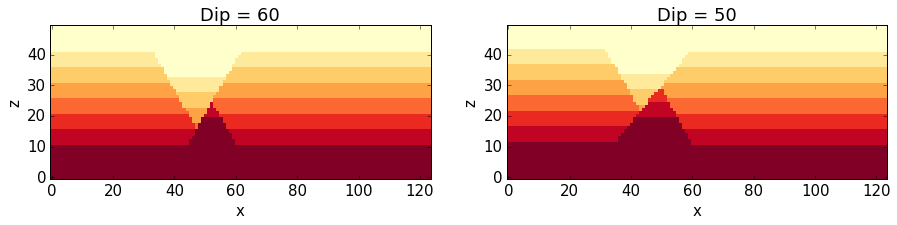
\includegraphics{3-Events_13_0.png}


\section{Changing the order of geological events}
\label{notebooks/3-Events:changing-the-order-of-geological-events}
The geological history is parameterised as single events in a timeline.
Changing the order of events can be performed with two basic methods:
\begin{enumerate}
\item {} 
Swapping two events with a simple command

\item {} 
Adjusting the entire timeline with a complete remapping of events

\end{enumerate}

The first method is probably the most useful to test how a simple change
in the order of events will effect the final geological model. We will
use it here with our example to test how the model would change if the
timing of the faults is swapped.

The method to swap two geological events is defined on the level of the
history object:

\begin{Verbatim}[commandchars=\\\{\}]
\PYG{n}{H1} \PYG{o}{=} \PYG{n}{pynoddy}\PYG{o}{.}\PYG{n}{history}\PYG{o}{.}\PYG{n}{NoddyHistory}\PYG{p}{(}\PYG{n}{history\PYGZus{}ori}\PYG{p}{)}
\end{Verbatim}

\begin{Verbatim}[commandchars=\\\{\}]
\PYG{c}{\PYGZsh{} The names of the two fault events defined in the history file are:}
\PYG{k}{print} \PYG{n}{H1}\PYG{o}{.}\PYG{n}{events}\PYG{p}{[}\PYG{l+m+mi}{2}\PYG{p}{]}\PYG{o}{.}\PYG{n}{name}
\PYG{k}{print} \PYG{n}{H1}\PYG{o}{.}\PYG{n}{events}\PYG{p}{[}\PYG{l+m+mi}{3}\PYG{p}{]}\PYG{o}{.}\PYG{n}{name}
\end{Verbatim}

\begin{Verbatim}[commandchars=\\\{\}]
\PYG{n}{Fault2}
\PYG{n}{Fault1}
\end{Verbatim}

We now swap the position of two events in the kinematic history. For
this purpose, a high-level function can directly be used:

\begin{Verbatim}[commandchars=\\\{\}]
\PYG{c}{\PYGZsh{} Now: swap the events:}
\PYG{n}{H1}\PYG{o}{.}\PYG{n}{swap\PYGZus{}events}\PYG{p}{(}\PYG{l+m+mi}{2}\PYG{p}{,}\PYG{l+m+mi}{3}\PYG{p}{)}
\end{Verbatim}

\begin{Verbatim}[commandchars=\\\{\}]
\PYG{c}{\PYGZsh{} And let\PYGZsq{}s check if this is correctly relfected in the events order now:}
\PYG{k}{print} \PYG{n}{H1}\PYG{o}{.}\PYG{n}{events}\PYG{p}{[}\PYG{l+m+mi}{2}\PYG{p}{]}\PYG{o}{.}\PYG{n}{name}
\PYG{k}{print} \PYG{n}{H1}\PYG{o}{.}\PYG{n}{events}\PYG{p}{[}\PYG{l+m+mi}{3}\PYG{p}{]}\PYG{o}{.}\PYG{n}{name}
\end{Verbatim}

\begin{Verbatim}[commandchars=\\\{\}]
\PYG{n}{Fault1}
\PYG{n}{Fault2}
\end{Verbatim}

Now let's create a new history file and evaluate the effect of the
changed order in a cross section view:

\begin{Verbatim}[commandchars=\\\{\}]
\PYG{n}{new\PYGZus{}history} \PYG{o}{=} \PYG{l+s}{\PYGZdq{}}\PYG{l+s}{faults\PYGZus{}changed\PYGZus{}order.his}\PYG{l+s}{\PYGZdq{}}
\PYG{n}{new\PYGZus{}output} \PYG{o}{=} \PYG{l+s}{\PYGZdq{}}\PYG{l+s}{faults\PYGZus{}out}\PYG{l+s}{\PYGZdq{}}
\PYG{n}{H1}\PYG{o}{.}\PYG{n}{write\PYGZus{}history}\PYG{p}{(}\PYG{n}{new\PYGZus{}history}\PYG{p}{)}
\PYG{n}{pynoddy}\PYG{o}{.}\PYG{n}{compute\PYGZus{}model}\PYG{p}{(}\PYG{n}{new\PYGZus{}history}\PYG{p}{,} \PYG{n}{new\PYGZus{}output}\PYG{p}{)}
\end{Verbatim}

\begin{Verbatim}[commandchars=\\\{\}]
\PYG{l+s}{\PYGZsq{}}\PYG{l+s}{\PYGZsq{}}
\end{Verbatim}

\begin{Verbatim}[commandchars=\\\{\}]
\PYG{n+nb}{reload}\PYG{p}{(}\PYG{n}{pynoddy}\PYG{o}{.}\PYG{n}{output}\PYG{p}{)}
\PYG{c}{\PYGZsh{} Load and compare both models}
\PYG{n}{NO1} \PYG{o}{=} \PYG{n}{pynoddy}\PYG{o}{.}\PYG{n}{output}\PYG{o}{.}\PYG{n}{NoddyOutput}\PYG{p}{(}\PYG{n}{output\PYGZus{}name}\PYG{p}{)}
\PYG{n}{NO2} \PYG{o}{=} \PYG{n}{pynoddy}\PYG{o}{.}\PYG{n}{output}\PYG{o}{.}\PYG{n}{NoddyOutput}\PYG{p}{(}\PYG{n}{new\PYGZus{}output}\PYG{p}{)}
\PYG{c}{\PYGZsh{} create basic figure layout}
\PYG{n}{fig} \PYG{o}{=} \PYG{n}{plt}\PYG{o}{.}\PYG{n}{figure}\PYG{p}{(}\PYG{n}{figsize} \PYG{o}{=} \PYG{p}{(}\PYG{l+m+mi}{15}\PYG{p}{,}\PYG{l+m+mi}{5}\PYG{p}{)}\PYG{p}{)}
\PYG{n}{ax1} \PYG{o}{=} \PYG{n}{fig}\PYG{o}{.}\PYG{n}{add\PYGZus{}subplot}\PYG{p}{(}\PYG{l+m+mi}{121}\PYG{p}{)}
\PYG{n}{ax2} \PYG{o}{=} \PYG{n}{fig}\PYG{o}{.}\PYG{n}{add\PYGZus{}subplot}\PYG{p}{(}\PYG{l+m+mi}{122}\PYG{p}{)}
\PYG{n}{NO1}\PYG{o}{.}\PYG{n}{plot\PYGZus{}section}\PYG{p}{(}\PYG{l+s}{\PYGZsq{}}\PYG{l+s}{y}\PYG{l+s}{\PYGZsq{}}\PYG{p}{,} \PYG{n}{ax} \PYG{o}{=} \PYG{n}{ax1}\PYG{p}{,} \PYG{n}{colorbar}\PYG{o}{=}\PYG{n+nb+bp}{False}\PYG{p}{,} \PYG{n}{title}\PYG{o}{=}\PYG{l+s}{\PYGZdq{}}\PYG{l+s}{Model 1}\PYG{l+s}{\PYGZdq{}}\PYG{p}{)}
\PYG{n}{NO2}\PYG{o}{.}\PYG{n}{plot\PYGZus{}section}\PYG{p}{(}\PYG{l+s}{\PYGZsq{}}\PYG{l+s}{y}\PYG{l+s}{\PYGZsq{}}\PYG{p}{,} \PYG{n}{ax} \PYG{o}{=} \PYG{n}{ax2}\PYG{p}{,} \PYG{n}{colorbar}\PYG{o}{=}\PYG{n+nb+bp}{False}\PYG{p}{,} \PYG{n}{title}\PYG{o}{=}\PYG{l+s}{\PYGZdq{}}\PYG{l+s}{Model 2}\PYG{l+s}{\PYGZdq{}}\PYG{p}{)}

\PYG{n}{plt}\PYG{o}{.}\PYG{n}{show}\PYG{p}{(}\PYG{p}{)}
\end{Verbatim}

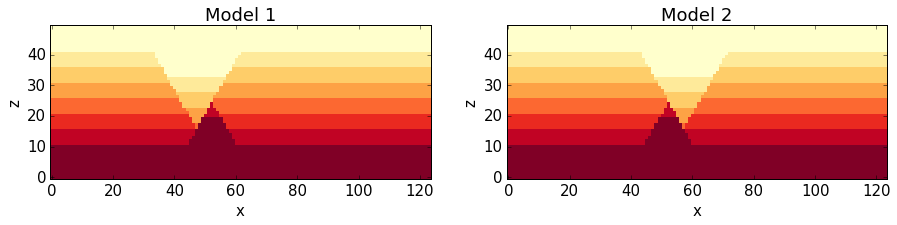
\includegraphics{3-Events_22_0.png}


\section{Determining the stratigraphic difference between two models}
\label{notebooks/3-Events:determining-the-stratigraphic-difference-between-two-models}
Just as another quick example of a possible application of pynoddy to
evaluate aspects that are not simply possible with, for example, the GUI
version of Noddy itself. In the last example with the changed order of
the faults, we might be interested to determine where in space this
change had an effect. We can test this quite simply using the
\code{NoddyOutput} objects.

The geology data is stored in the \code{NoddyOutput.block} attribute. To
evaluate the difference between two models, we can therefore simply
compute:

\begin{Verbatim}[commandchars=\\\{\}]
\PYG{n}{diff} \PYG{o}{=} \PYG{p}{(}\PYG{n}{NO2}\PYG{o}{.}\PYG{n}{block} \PYG{o}{\PYGZhy{}} \PYG{n}{NO1}\PYG{o}{.}\PYG{n}{block}\PYG{p}{)}
\end{Verbatim}

And create a simple visualisation of the difference in a slice plot
with:

\begin{Verbatim}[commandchars=\\\{\}]
\PYG{n}{fig} \PYG{o}{=} \PYG{n}{plt}\PYG{o}{.}\PYG{n}{figure}\PYG{p}{(}\PYG{n}{figsize} \PYG{o}{=} \PYG{p}{(}\PYG{l+m+mi}{5}\PYG{p}{,}\PYG{l+m+mi}{3}\PYG{p}{)}\PYG{p}{)}
\PYG{n}{ax} \PYG{o}{=} \PYG{n}{fig}\PYG{o}{.}\PYG{n}{add\PYGZus{}subplot}\PYG{p}{(}\PYG{l+m+mi}{111}\PYG{p}{)}
\PYG{n}{ax}\PYG{o}{.}\PYG{n}{imshow}\PYG{p}{(}\PYG{n}{diff}\PYG{p}{[}\PYG{p}{:}\PYG{p}{,}\PYG{l+m+mi}{10}\PYG{p}{,}\PYG{p}{:}\PYG{p}{]}\PYG{o}{.}\PYG{n}{transpose}\PYG{p}{(}\PYG{p}{)}\PYG{p}{,} \PYG{n}{interpolation}\PYG{o}{=}\PYG{l+s}{\PYGZsq{}}\PYG{l+s}{nearest}\PYG{l+s}{\PYGZsq{}}\PYG{p}{,}
          \PYG{n}{cmap} \PYG{o}{=} \PYG{l+s}{\PYGZdq{}}\PYG{l+s}{RdBu}\PYG{l+s}{\PYGZdq{}}\PYG{p}{,} \PYG{n}{origin} \PYG{o}{=} \PYG{l+s}{\PYGZsq{}}\PYG{l+s}{lower left}\PYG{l+s}{\PYGZsq{}}\PYG{p}{)}
\end{Verbatim}

\begin{Verbatim}[commandchars=\\\{\}]
\PYGZlt{}matplotlib.image.AxesImage at 0x10cf3be10\PYGZgt{}
\end{Verbatim}

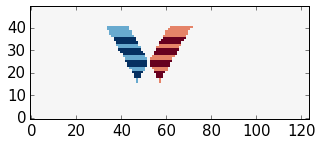
\includegraphics{3-Events_26_1.png}

(Adding a meaningful title and axis labels to the plot is left to the
reader as simple excercise :-) Future versions of pynoddy might provide
an automatic implementation for this step...)

Again, we may want to visualise results in 3-D. We can use the
\code{export\_to\_vtk}-function as before, but now assing the data array to
be exported as the calulcated differnce field:

\begin{Verbatim}[commandchars=\\\{\}]
\PYG{n}{NO1}\PYG{o}{.}\PYG{n}{export\PYGZus{}to\PYGZus{}vtk}\PYG{p}{(}\PYG{n}{vtk\PYGZus{}filename} \PYG{o}{=} \PYG{l+s}{\PYGZdq{}}\PYG{l+s}{model\PYGZus{}diff}\PYG{l+s}{\PYGZdq{}}\PYG{p}{,} \PYG{n}{data} \PYG{o}{=} \PYG{n}{diff}\PYG{p}{)}
\end{Verbatim}

A 3-D view of the difference plot is presented below.
\begin{figure}[htbp]
\centering
\capstart

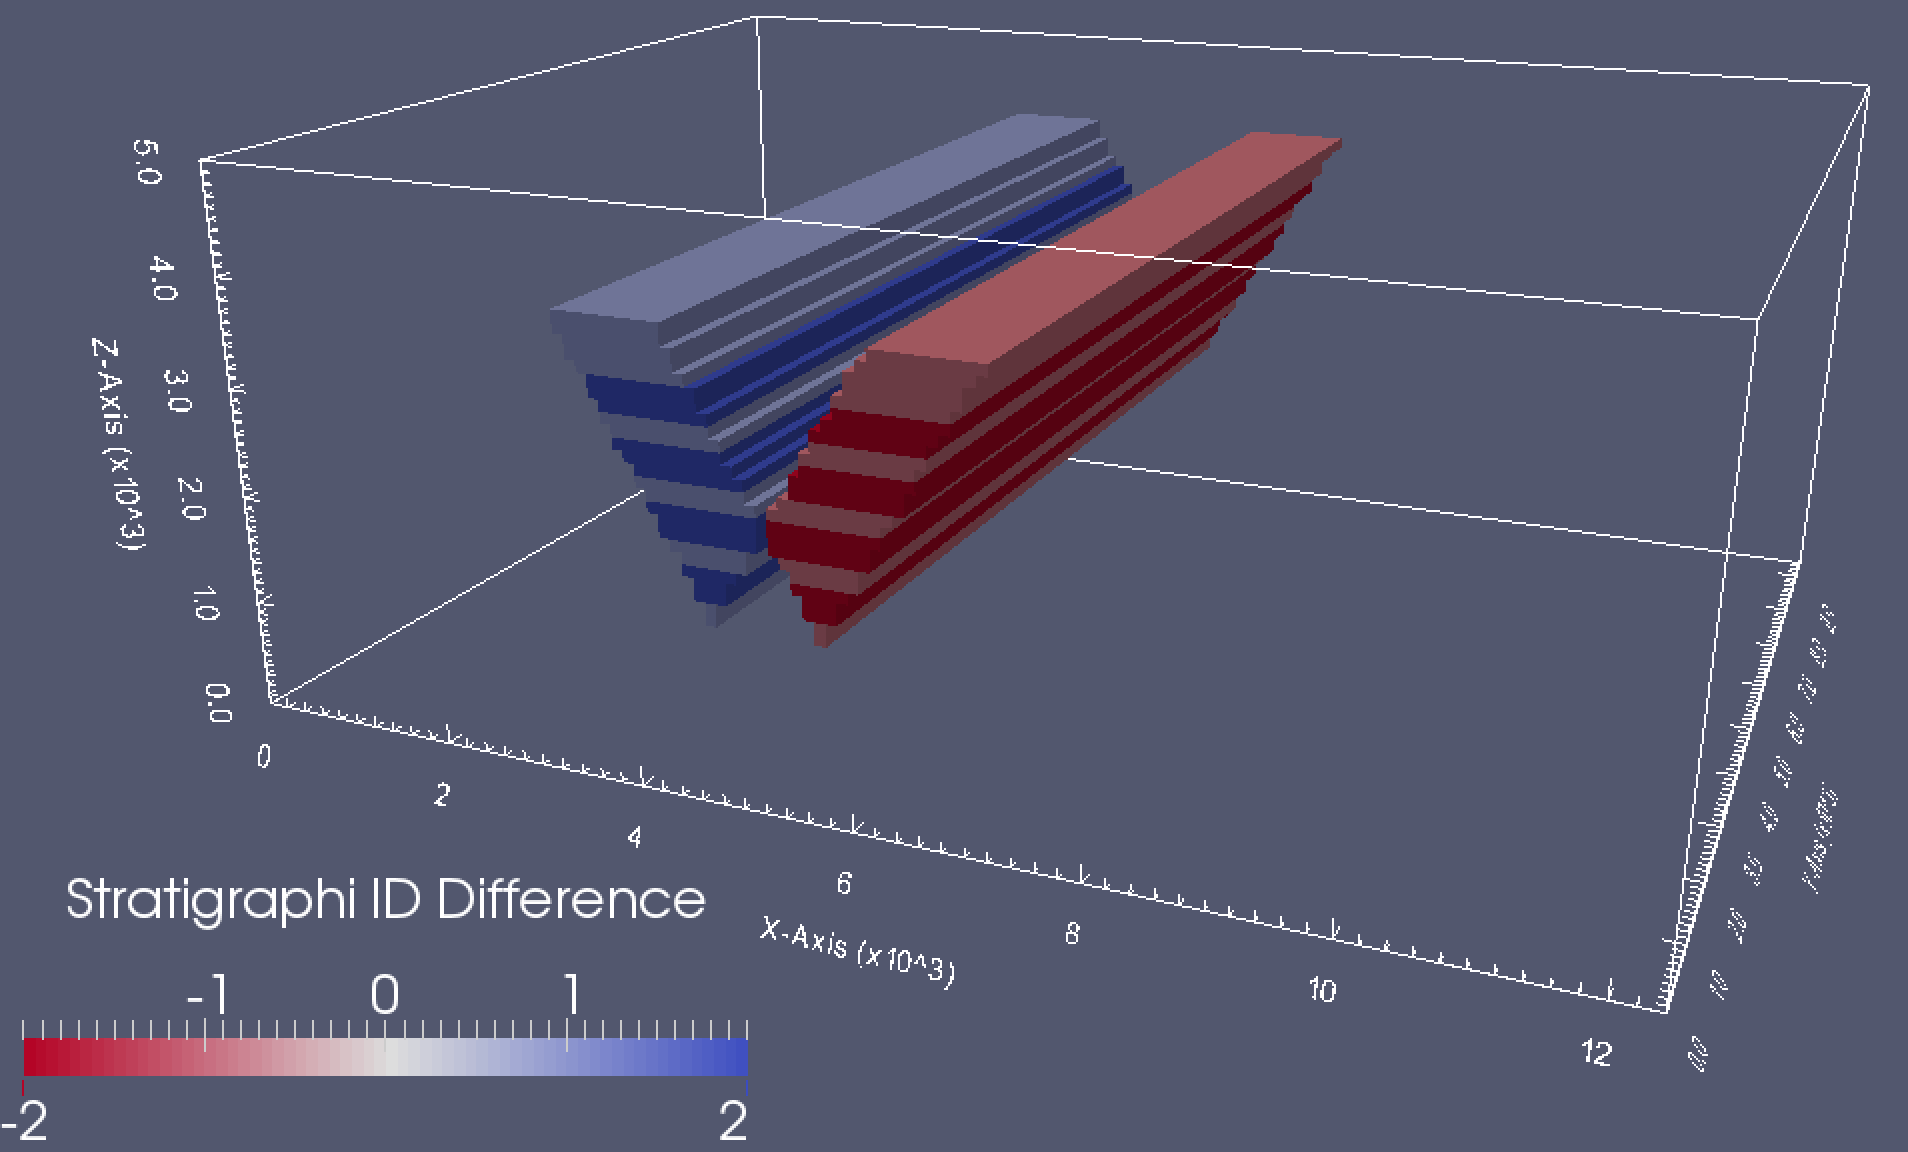
\includegraphics{diff_3d_3.png}
\caption{3-D visualisation of stratigraphic id difference}\end{figure}


\chapter{Creating a model from scratch}
\label{notebooks/4-Create-model:creating-a-model-from-scratch}\label{notebooks/4-Create-model::doc}
We describe here how to generate a simple history file for computation
with Noddy using the functionality of pynoddy. If possible, it is
advisable to generate the history files with the Windows GUI for Noddy
as this method provides, to date, a simpler and more complete interface
to the entire functionality.

For completeness, pynoddy contains the functionality to generate simple
models, for example to automate the model construction process, or to
enable the model construction for users who are not running Windows.
Some simple examlpes are shown in the following.

\begin{Verbatim}[commandchars=\\\{\}]
\PYG{k+kn}{from} \PYG{n+nn}{matplotlib} \PYG{k+kn}{import} \PYG{n}{rc\PYGZus{}params}
\end{Verbatim}

\begin{Verbatim}[commandchars=\\\{\}]
\PYG{k+kn}{from} \PYG{n+nn}{IPython.core.display} \PYG{k+kn}{import} \PYG{n}{HTML}
\PYG{n}{css\PYGZus{}file} \PYG{o}{=} \PYG{l+s}{\PYGZsq{}}\PYG{l+s}{pynoddy.css}\PYG{l+s}{\PYGZsq{}}
\PYG{n}{HTML}\PYG{p}{(}\PYG{n+nb}{open}\PYG{p}{(}\PYG{n}{css\PYGZus{}file}\PYG{p}{,} \PYG{l+s}{\PYGZdq{}}\PYG{l+s}{r}\PYG{l+s}{\PYGZdq{}}\PYG{p}{)}\PYG{o}{.}\PYG{n}{read}\PYG{p}{(}\PYG{p}{)}\PYG{p}{)}
\end{Verbatim}

\begin{Verbatim}[commandchars=\\\{\}]
\PYG{k+kn}{import} \PYG{n+nn}{sys}\PYG{o}{,} \PYG{n+nn}{os}
\PYG{k+kn}{import} \PYG{n+nn}{matplotlib.pyplot} \PYG{k+kn}{as} \PYG{n+nn}{plt}
\PYG{c}{\PYGZsh{} adjust some settings for matplotlib}
\PYG{k+kn}{from} \PYG{n+nn}{matplotlib} \PYG{k+kn}{import} \PYG{n}{rcParams}
\PYG{c}{\PYGZsh{} print rcParams}
\PYG{n}{rcParams}\PYG{p}{[}\PYG{l+s}{\PYGZsq{}}\PYG{l+s}{font.size}\PYG{l+s}{\PYGZsq{}}\PYG{p}{]} \PYG{o}{=} \PYG{l+m+mi}{15}
\PYG{c}{\PYGZsh{} determine path of repository to set paths corretly below}
\PYG{n}{repo\PYGZus{}path} \PYG{o}{=} \PYG{n}{os}\PYG{o}{.}\PYG{n}{path}\PYG{o}{.}\PYG{n}{realpath}\PYG{p}{(}\PYG{l+s}{\PYGZsq{}}\PYG{l+s}{../..}\PYG{l+s}{\PYGZsq{}}\PYG{p}{)}
\PYG{k+kn}{import} \PYG{n+nn}{pynoddy.history}
\end{Verbatim}

\begin{Verbatim}[commandchars=\\\{\}]
\PYGZpc{}matplotlib inline
\end{Verbatim}

\begin{Verbatim}[commandchars=\\\{\}]
\PYG{n}{rcParams}\PYG{o}{.}\PYG{n}{update}\PYG{p}{(}\PYG{p}{\PYGZob{}}\PYG{l+s}{\PYGZsq{}}\PYG{l+s}{font.size}\PYG{l+s}{\PYGZsq{}}\PYG{p}{:} \PYG{l+m+mi}{20}\PYG{p}{\PYGZcb{}}\PYG{p}{)}
\end{Verbatim}


\section{Defining a stratigraphy}
\label{notebooks/4-Create-model:defining-a-stratigraphy}
We start with the definition of a (base) stratigraphy for the model.

\begin{Verbatim}[commandchars=\\\{\}]
\PYG{c}{\PYGZsh{} Combined: model generation and output vis to test:}
\PYG{n}{history} \PYG{o}{=} \PYG{l+s}{\PYGZdq{}}\PYG{l+s}{simple\PYGZus{}model.his}\PYG{l+s}{\PYGZdq{}}
\PYG{n}{output\PYGZus{}name} \PYG{o}{=} \PYG{l+s}{\PYGZdq{}}\PYG{l+s}{simple\PYGZus{}out}\PYG{l+s}{\PYGZdq{}}
\PYG{n+nb}{reload}\PYG{p}{(}\PYG{n}{pynoddy}\PYG{o}{.}\PYG{n}{history}\PYG{p}{)}
\PYG{n+nb}{reload}\PYG{p}{(}\PYG{n}{pynoddy}\PYG{o}{.}\PYG{n}{events}\PYG{p}{)}

\PYG{c}{\PYGZsh{} create pynoddy object}
\PYG{n}{nm} \PYG{o}{=} \PYG{n}{pynoddy}\PYG{o}{.}\PYG{n}{history}\PYG{o}{.}\PYG{n}{NoddyHistory}\PYG{p}{(}\PYG{p}{)}
\PYG{c}{\PYGZsh{} add stratigraphy}
\PYG{n}{strati\PYGZus{}options} \PYG{o}{=} \PYG{p}{\PYGZob{}}\PYG{l+s}{\PYGZsq{}}\PYG{l+s}{num\PYGZus{}layers}\PYG{l+s}{\PYGZsq{}} \PYG{p}{:} \PYG{l+m+mi}{8}\PYG{p}{,}
                  \PYG{l+s}{\PYGZsq{}}\PYG{l+s}{layer\PYGZus{}names}\PYG{l+s}{\PYGZsq{}} \PYG{p}{:} \PYG{p}{[}\PYG{l+s}{\PYGZsq{}}\PYG{l+s}{layer 1}\PYG{l+s}{\PYGZsq{}}\PYG{p}{,} \PYG{l+s}{\PYGZsq{}}\PYG{l+s}{layer 2}\PYG{l+s}{\PYGZsq{}}\PYG{p}{,} \PYG{l+s}{\PYGZsq{}}\PYG{l+s}{layer 3}\PYG{l+s}{\PYGZsq{}}\PYG{p}{,}
                                   \PYG{l+s}{\PYGZsq{}}\PYG{l+s}{layer 4}\PYG{l+s}{\PYGZsq{}}\PYG{p}{,} \PYG{l+s}{\PYGZsq{}}\PYG{l+s}{layer 5}\PYG{l+s}{\PYGZsq{}}\PYG{p}{,} \PYG{l+s}{\PYGZsq{}}\PYG{l+s}{layer 6}\PYG{l+s}{\PYGZsq{}}\PYG{p}{,}
                                   \PYG{l+s}{\PYGZsq{}}\PYG{l+s}{layer 7}\PYG{l+s}{\PYGZsq{}}\PYG{p}{,} \PYG{l+s}{\PYGZsq{}}\PYG{l+s}{layer 8}\PYG{l+s}{\PYGZsq{}}\PYG{p}{]}\PYG{p}{,}
                  \PYG{l+s}{\PYGZsq{}}\PYG{l+s}{layer\PYGZus{}thickness}\PYG{l+s}{\PYGZsq{}} \PYG{p}{:} \PYG{p}{[}\PYG{l+m+mi}{1500}\PYG{p}{,} \PYG{l+m+mi}{500}\PYG{p}{,} \PYG{l+m+mi}{500}\PYG{p}{,} \PYG{l+m+mi}{500}\PYG{p}{,} \PYG{l+m+mi}{500}\PYG{p}{,} \PYG{l+m+mi}{500}\PYG{p}{,} \PYG{l+m+mi}{500}\PYG{p}{,} \PYG{l+m+mi}{500}\PYG{p}{]}\PYG{p}{\PYGZcb{}}
\PYG{n}{nm}\PYG{o}{.}\PYG{n}{add\PYGZus{}event}\PYG{p}{(}\PYG{l+s}{\PYGZsq{}}\PYG{l+s}{stratigraphy}\PYG{l+s}{\PYGZsq{}}\PYG{p}{,} \PYG{n}{strati\PYGZus{}options} \PYG{p}{)}

\PYG{n}{nm}\PYG{o}{.}\PYG{n}{write\PYGZus{}history}\PYG{p}{(}\PYG{n}{history}\PYG{p}{)}
\end{Verbatim}

\begin{Verbatim}[commandchars=\\\{\}]
\PYG{c}{\PYGZsh{} Compute the model}
\PYG{n+nb}{reload}\PYG{p}{(}\PYG{n}{pynoddy}\PYG{p}{)}
\PYG{n}{pynoddy}\PYG{o}{.}\PYG{n}{compute\PYGZus{}model}\PYG{p}{(}\PYG{n}{history}\PYG{p}{,} \PYG{n}{output\PYGZus{}name}\PYG{p}{)}
\end{Verbatim}

\begin{Verbatim}[commandchars=\\\{\}]
\PYG{l+s}{\PYGZsq{}}\PYG{l+s}{\PYGZsq{}}
\end{Verbatim}

\begin{Verbatim}[commandchars=\\\{\}]
\PYG{c}{\PYGZsh{} Plot output}
\PYG{k+kn}{import} \PYG{n+nn}{pynoddy.output}
\PYG{n+nb}{reload}\PYG{p}{(}\PYG{n}{pynoddy}\PYG{o}{.}\PYG{n}{output}\PYG{p}{)}
\PYG{n}{nout} \PYG{o}{=} \PYG{n}{pynoddy}\PYG{o}{.}\PYG{n}{output}\PYG{o}{.}\PYG{n}{NoddyOutput}\PYG{p}{(}\PYG{n}{output\PYGZus{}name}\PYG{p}{)}
\PYG{n}{nout}\PYG{o}{.}\PYG{n}{plot\PYGZus{}section}\PYG{p}{(}\PYG{l+s}{\PYGZsq{}}\PYG{l+s}{y}\PYG{l+s}{\PYGZsq{}}\PYG{p}{,} \PYG{n}{layer\PYGZus{}labels} \PYG{o}{=} \PYG{n}{strati\PYGZus{}options}\PYG{p}{[}\PYG{l+s}{\PYGZsq{}}\PYG{l+s}{layer\PYGZus{}names}\PYG{l+s}{\PYGZsq{}}\PYG{p}{]}\PYG{p}{[}\PYG{p}{:}\PYG{p}{:}\PYG{o}{\PYGZhy{}}\PYG{l+m+mi}{1}\PYG{p}{]}\PYG{p}{,}
                  \PYG{n}{colorbar} \PYG{o}{=} \PYG{n+nb+bp}{True}\PYG{p}{,} \PYG{n}{title}\PYG{o}{=}\PYG{l+s}{\PYGZdq{}}\PYG{l+s}{\PYGZdq{}}\PYG{p}{,}
                  \PYG{n}{savefig} \PYG{o}{=} \PYG{n+nb+bp}{False}\PYG{p}{,} \PYG{n}{fig\PYGZus{}filename} \PYG{o}{=} \PYG{l+s}{\PYGZdq{}}\PYG{l+s}{ex01\PYGZus{}strati.eps}\PYG{l+s}{\PYGZdq{}}\PYG{p}{)}
\end{Verbatim}

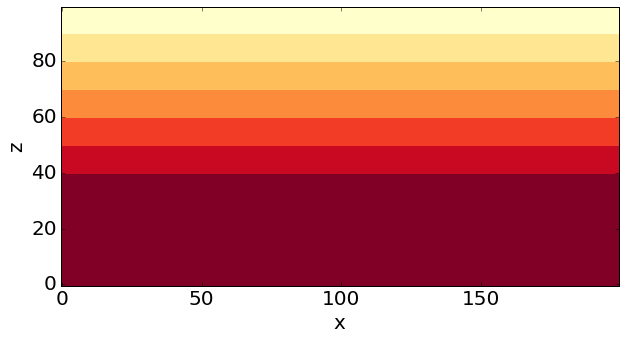
\includegraphics{4-Create-model_9_0.png}


\section{Add a fault event}
\label{notebooks/4-Create-model:add-a-fault-event}
As a next step, let's now add the faults to the model.

\begin{Verbatim}[commandchars=\\\{\}]
\PYG{n+nb}{reload}\PYG{p}{(}\PYG{n}{pynoddy}\PYG{o}{.}\PYG{n}{history}\PYG{p}{)}
\PYG{n+nb}{reload}\PYG{p}{(}\PYG{n}{pynoddy}\PYG{o}{.}\PYG{n}{events}\PYG{p}{)}
\PYG{n}{nm} \PYG{o}{=} \PYG{n}{pynoddy}\PYG{o}{.}\PYG{n}{history}\PYG{o}{.}\PYG{n}{NoddyHistory}\PYG{p}{(}\PYG{p}{)}
\PYG{c}{\PYGZsh{} add stratigraphy}
\PYG{n}{strati\PYGZus{}options} \PYG{o}{=} \PYG{p}{\PYGZob{}}\PYG{l+s}{\PYGZsq{}}\PYG{l+s}{num\PYGZus{}layers}\PYG{l+s}{\PYGZsq{}} \PYG{p}{:} \PYG{l+m+mi}{8}\PYG{p}{,}
                  \PYG{l+s}{\PYGZsq{}}\PYG{l+s}{layer\PYGZus{}names}\PYG{l+s}{\PYGZsq{}} \PYG{p}{:} \PYG{p}{[}\PYG{l+s}{\PYGZsq{}}\PYG{l+s}{layer 1}\PYG{l+s}{\PYGZsq{}}\PYG{p}{,} \PYG{l+s}{\PYGZsq{}}\PYG{l+s}{layer 2}\PYG{l+s}{\PYGZsq{}}\PYG{p}{,} \PYG{l+s}{\PYGZsq{}}\PYG{l+s}{layer 3}\PYG{l+s}{\PYGZsq{}}\PYG{p}{,} \PYG{l+s}{\PYGZsq{}}\PYG{l+s}{layer 4}\PYG{l+s}{\PYGZsq{}}\PYG{p}{,} \PYG{l+s}{\PYGZsq{}}\PYG{l+s}{layer 5}\PYG{l+s}{\PYGZsq{}}\PYG{p}{,} \PYG{l+s}{\PYGZsq{}}\PYG{l+s}{layer 6}\PYG{l+s}{\PYGZsq{}}\PYG{p}{,} \PYG{l+s}{\PYGZsq{}}\PYG{l+s}{layer 7}\PYG{l+s}{\PYGZsq{}}\PYG{p}{,} \PYG{l+s}{\PYGZsq{}}\PYG{l+s}{layer 8}\PYG{l+s}{\PYGZsq{}}\PYG{p}{]}\PYG{p}{,}
                  \PYG{l+s}{\PYGZsq{}}\PYG{l+s}{layer\PYGZus{}thickness}\PYG{l+s}{\PYGZsq{}} \PYG{p}{:} \PYG{p}{[}\PYG{l+m+mi}{1500}\PYG{p}{,} \PYG{l+m+mi}{500}\PYG{p}{,} \PYG{l+m+mi}{500}\PYG{p}{,} \PYG{l+m+mi}{500}\PYG{p}{,} \PYG{l+m+mi}{500}\PYG{p}{,} \PYG{l+m+mi}{500}\PYG{p}{,} \PYG{l+m+mi}{500}\PYG{p}{,} \PYG{l+m+mi}{500}\PYG{p}{]}\PYG{p}{\PYGZcb{}}
\PYG{n}{nm}\PYG{o}{.}\PYG{n}{add\PYGZus{}event}\PYG{p}{(}\PYG{l+s}{\PYGZsq{}}\PYG{l+s}{stratigraphy}\PYG{l+s}{\PYGZsq{}}\PYG{p}{,} \PYG{n}{strati\PYGZus{}options} \PYG{p}{)}




\PYG{c}{\PYGZsh{} The following options define the fault geometry:}
\PYG{n}{fault\PYGZus{}options} \PYG{o}{=} \PYG{p}{\PYGZob{}}\PYG{l+s}{\PYGZsq{}}\PYG{l+s}{name}\PYG{l+s}{\PYGZsq{}} \PYG{p}{:} \PYG{l+s}{\PYGZsq{}}\PYG{l+s}{Fault\PYGZus{}E}\PYG{l+s}{\PYGZsq{}}\PYG{p}{,}
                 \PYG{l+s}{\PYGZsq{}}\PYG{l+s}{pos}\PYG{l+s}{\PYGZsq{}} \PYG{p}{:} \PYG{p}{(}\PYG{l+m+mi}{6000}\PYG{p}{,} \PYG{l+m+mi}{0}\PYG{p}{,} \PYG{l+m+mi}{5000}\PYG{p}{)}\PYG{p}{,}
                 \PYG{l+s}{\PYGZsq{}}\PYG{l+s}{dip\PYGZus{}dir}\PYG{l+s}{\PYGZsq{}} \PYG{p}{:} \PYG{l+m+mi}{270}\PYG{p}{,}
                 \PYG{l+s}{\PYGZsq{}}\PYG{l+s}{dip}\PYG{l+s}{\PYGZsq{}} \PYG{p}{:} \PYG{l+m+mi}{60}\PYG{p}{,}
                 \PYG{l+s}{\PYGZsq{}}\PYG{l+s}{slip}\PYG{l+s}{\PYGZsq{}} \PYG{p}{:} \PYG{l+m+mi}{1000}\PYG{p}{\PYGZcb{}}

\PYG{n}{nm}\PYG{o}{.}\PYG{n}{add\PYGZus{}event}\PYG{p}{(}\PYG{l+s}{\PYGZsq{}}\PYG{l+s}{fault}\PYG{l+s}{\PYGZsq{}}\PYG{p}{,} \PYG{n}{fault\PYGZus{}options}\PYG{p}{)}
\end{Verbatim}

\begin{Verbatim}[commandchars=\\\{\}]
\PYG{n}{nm}\PYG{o}{.}\PYG{n}{events}
\end{Verbatim}

\begin{Verbatim}[commandchars=\\\{\}]
\PYGZob{}1: \PYGZlt{}pynoddy.events.Stratigraphy at 0x1073fc590\PYGZgt{},
 2: \PYGZlt{}pynoddy.events.Fault at 0x107565fd0\PYGZgt{}\PYGZcb{}
\end{Verbatim}

\begin{Verbatim}[commandchars=\\\{\}]
\PYG{n}{nm}\PYG{o}{.}\PYG{n}{write\PYGZus{}history}\PYG{p}{(}\PYG{n}{history}\PYG{p}{)}
\end{Verbatim}

\begin{Verbatim}[commandchars=\\\{\}]
\PYG{c}{\PYGZsh{} Compute the model}
\PYG{n}{pynoddy}\PYG{o}{.}\PYG{n}{compute\PYGZus{}model}\PYG{p}{(}\PYG{n}{history}\PYG{p}{,} \PYG{n}{output\PYGZus{}name}\PYG{p}{)}
\end{Verbatim}

\begin{Verbatim}[commandchars=\\\{\}]
\PYG{l+s}{\PYGZsq{}}\PYG{l+s}{\PYGZsq{}}
\end{Verbatim}

\begin{Verbatim}[commandchars=\\\{\}]
\PYG{c}{\PYGZsh{} Plot output}
\PYG{n+nb}{reload}\PYG{p}{(}\PYG{n}{pynoddy}\PYG{o}{.}\PYG{n}{output}\PYG{p}{)}
\PYG{n}{nout} \PYG{o}{=} \PYG{n}{pynoddy}\PYG{o}{.}\PYG{n}{output}\PYG{o}{.}\PYG{n}{NoddyOutput}\PYG{p}{(}\PYG{n}{output\PYGZus{}name}\PYG{p}{)}
\PYG{n}{nout}\PYG{o}{.}\PYG{n}{plot\PYGZus{}section}\PYG{p}{(}\PYG{l+s}{\PYGZsq{}}\PYG{l+s}{y}\PYG{l+s}{\PYGZsq{}}\PYG{p}{,} \PYG{n}{layer\PYGZus{}labels} \PYG{o}{=} \PYG{n}{strati\PYGZus{}options}\PYG{p}{[}\PYG{l+s}{\PYGZsq{}}\PYG{l+s}{layer\PYGZus{}names}\PYG{l+s}{\PYGZsq{}}\PYG{p}{]}\PYG{p}{[}\PYG{p}{:}\PYG{p}{:}\PYG{o}{\PYGZhy{}}\PYG{l+m+mi}{1}\PYG{p}{]}\PYG{p}{,}
                  \PYG{n}{colorbar} \PYG{o}{=} \PYG{n+nb+bp}{True}\PYG{p}{,} \PYG{n}{title} \PYG{o}{=} \PYG{l+s}{\PYGZdq{}}\PYG{l+s}{\PYGZdq{}}\PYG{p}{,}
                  \PYG{n}{savefig} \PYG{o}{=} \PYG{n+nb+bp}{False}\PYG{p}{,} \PYG{n}{fig\PYGZus{}filename} \PYG{o}{=} \PYG{l+s}{\PYGZdq{}}\PYG{l+s}{ex01\PYGZus{}fault\PYGZus{}E.eps}\PYG{l+s}{\PYGZdq{}}\PYG{p}{)}
\end{Verbatim}

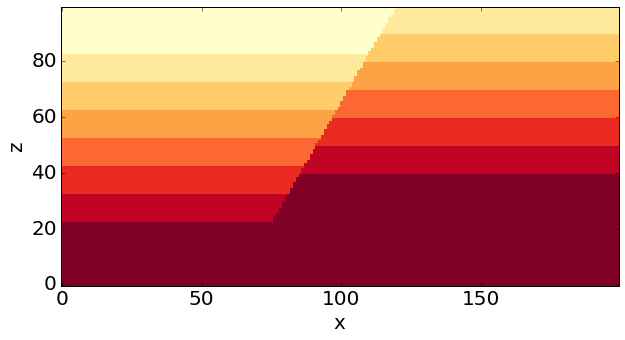
\includegraphics{4-Create-model_15_0.png}

\begin{Verbatim}[commandchars=\\\{\}]
\PYG{c}{\PYGZsh{} The following options define the fault geometry:}
\PYG{n}{fault\PYGZus{}options} \PYG{o}{=} \PYG{p}{\PYGZob{}}\PYG{l+s}{\PYGZsq{}}\PYG{l+s}{name}\PYG{l+s}{\PYGZsq{}} \PYG{p}{:} \PYG{l+s}{\PYGZsq{}}\PYG{l+s}{Fault\PYGZus{}1}\PYG{l+s}{\PYGZsq{}}\PYG{p}{,}
                 \PYG{l+s}{\PYGZsq{}}\PYG{l+s}{pos}\PYG{l+s}{\PYGZsq{}} \PYG{p}{:} \PYG{p}{(}\PYG{l+m+mi}{5500}\PYG{p}{,} \PYG{l+m+mi}{3500}\PYG{p}{,} \PYG{l+m+mi}{0}\PYG{p}{)}\PYG{p}{,}
                 \PYG{l+s}{\PYGZsq{}}\PYG{l+s}{dip\PYGZus{}dir}\PYG{l+s}{\PYGZsq{}} \PYG{p}{:} \PYG{l+m+mi}{270}\PYG{p}{,}
                 \PYG{l+s}{\PYGZsq{}}\PYG{l+s}{dip}\PYG{l+s}{\PYGZsq{}} \PYG{p}{:} \PYG{l+m+mi}{60}\PYG{p}{,}
                 \PYG{l+s}{\PYGZsq{}}\PYG{l+s}{slip}\PYG{l+s}{\PYGZsq{}} \PYG{p}{:} \PYG{l+m+mi}{1000}\PYG{p}{\PYGZcb{}}

\PYG{n}{nm}\PYG{o}{.}\PYG{n}{add\PYGZus{}event}\PYG{p}{(}\PYG{l+s}{\PYGZsq{}}\PYG{l+s}{fault}\PYG{l+s}{\PYGZsq{}}\PYG{p}{,} \PYG{n}{fault\PYGZus{}options}\PYG{p}{)}
\end{Verbatim}

\begin{Verbatim}[commandchars=\\\{\}]
\PYG{n}{nm}\PYG{o}{.}\PYG{n}{write\PYGZus{}history}\PYG{p}{(}\PYG{n}{history}\PYG{p}{)}
\end{Verbatim}

\begin{Verbatim}[commandchars=\\\{\}]
\PYG{c}{\PYGZsh{} Compute the model}
\PYG{n}{pynoddy}\PYG{o}{.}\PYG{n}{compute\PYGZus{}model}\PYG{p}{(}\PYG{n}{history}\PYG{p}{,} \PYG{n}{output\PYGZus{}name}\PYG{p}{)}
\end{Verbatim}

\begin{Verbatim}[commandchars=\\\{\}]
\PYG{l+s}{\PYGZsq{}}\PYG{l+s}{\PYGZsq{}}
\end{Verbatim}

\begin{Verbatim}[commandchars=\\\{\}]
\PYG{c}{\PYGZsh{} Plot output}
\PYG{n+nb}{reload}\PYG{p}{(}\PYG{n}{pynoddy}\PYG{o}{.}\PYG{n}{output}\PYG{p}{)}
\PYG{n}{nout} \PYG{o}{=} \PYG{n}{pynoddy}\PYG{o}{.}\PYG{n}{output}\PYG{o}{.}\PYG{n}{NoddyOutput}\PYG{p}{(}\PYG{n}{output\PYGZus{}name}\PYG{p}{)}
\PYG{n}{nout}\PYG{o}{.}\PYG{n}{plot\PYGZus{}section}\PYG{p}{(}\PYG{l+s}{\PYGZsq{}}\PYG{l+s}{y}\PYG{l+s}{\PYGZsq{}}\PYG{p}{,} \PYG{n}{layer\PYGZus{}labels} \PYG{o}{=} \PYG{n}{strati\PYGZus{}options}\PYG{p}{[}\PYG{l+s}{\PYGZsq{}}\PYG{l+s}{layer\PYGZus{}names}\PYG{l+s}{\PYGZsq{}}\PYG{p}{]}\PYG{p}{[}\PYG{p}{:}\PYG{p}{:}\PYG{o}{\PYGZhy{}}\PYG{l+m+mi}{1}\PYG{p}{]}\PYG{p}{,} \PYG{n}{colorbar} \PYG{o}{=} \PYG{n+nb+bp}{True}\PYG{p}{)}
\end{Verbatim}

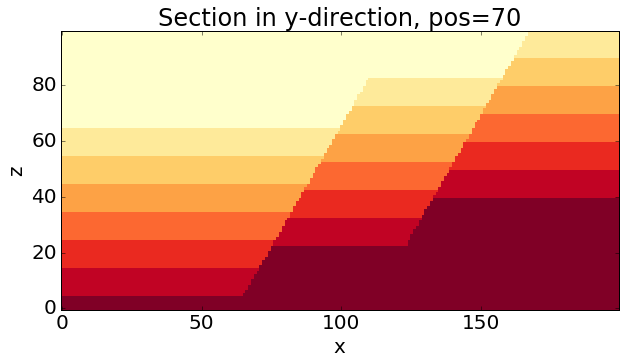
\includegraphics{4-Create-model_19_0.png}

\begin{Verbatim}[commandchars=\\\{\}]
\PYG{n}{nm1} \PYG{o}{=} \PYG{n}{pynoddy}\PYG{o}{.}\PYG{n}{history}\PYG{o}{.}\PYG{n}{NoddyHistory}\PYG{p}{(}\PYG{n}{history}\PYG{p}{)}
\end{Verbatim}

\begin{Verbatim}[commandchars=\\\{\}]
\PYG{n}{nm1}\PYG{o}{.}\PYG{n}{get\PYGZus{}extent}\PYG{p}{(}\PYG{p}{)}
\end{Verbatim}

\begin{Verbatim}[commandchars=\\\{\}]
\PYG{p}{(}\PYG{l+m+mf}{10000.0}\PYG{p}{,} \PYG{l+m+mf}{7000.0}\PYG{p}{,} \PYG{l+m+mf}{5000.0}\PYG{p}{)}
\end{Verbatim}


\section{Complete Model Set-up}
\label{notebooks/4-Create-model:complete-model-set-up}
And here now, combining all the previous steps, the entire model set-up
with base stratigraphy and two faults:

\begin{Verbatim}[commandchars=\\\{\}]
\PYG{n+nb}{reload}\PYG{p}{(}\PYG{n}{pynoddy}\PYG{o}{.}\PYG{n}{history}\PYG{p}{)}
\PYG{n+nb}{reload}\PYG{p}{(}\PYG{n}{pynoddy}\PYG{o}{.}\PYG{n}{events}\PYG{p}{)}
\PYG{n}{nm} \PYG{o}{=} \PYG{n}{pynoddy}\PYG{o}{.}\PYG{n}{history}\PYG{o}{.}\PYG{n}{NoddyHistory}\PYG{p}{(}\PYG{p}{)}
\PYG{c}{\PYGZsh{} add stratigraphy}
\PYG{n}{strati\PYGZus{}options} \PYG{o}{=} \PYG{p}{\PYGZob{}}\PYG{l+s}{\PYGZsq{}}\PYG{l+s}{num\PYGZus{}layers}\PYG{l+s}{\PYGZsq{}} \PYG{p}{:} \PYG{l+m+mi}{8}\PYG{p}{,}
                  \PYG{l+s}{\PYGZsq{}}\PYG{l+s}{layer\PYGZus{}names}\PYG{l+s}{\PYGZsq{}} \PYG{p}{:} \PYG{p}{[}\PYG{l+s}{\PYGZsq{}}\PYG{l+s}{layer 1}\PYG{l+s}{\PYGZsq{}}\PYG{p}{,} \PYG{l+s}{\PYGZsq{}}\PYG{l+s}{layer 2}\PYG{l+s}{\PYGZsq{}}\PYG{p}{,} \PYG{l+s}{\PYGZsq{}}\PYG{l+s}{layer 3}\PYG{l+s}{\PYGZsq{}}\PYG{p}{,}
                                   \PYG{l+s}{\PYGZsq{}}\PYG{l+s}{layer 4}\PYG{l+s}{\PYGZsq{}}\PYG{p}{,} \PYG{l+s}{\PYGZsq{}}\PYG{l+s}{layer 5}\PYG{l+s}{\PYGZsq{}}\PYG{p}{,} \PYG{l+s}{\PYGZsq{}}\PYG{l+s}{layer 6}\PYG{l+s}{\PYGZsq{}}\PYG{p}{,}
                                   \PYG{l+s}{\PYGZsq{}}\PYG{l+s}{layer 7}\PYG{l+s}{\PYGZsq{}}\PYG{p}{,} \PYG{l+s}{\PYGZsq{}}\PYG{l+s}{layer 8}\PYG{l+s}{\PYGZsq{}}\PYG{p}{]}\PYG{p}{,}
                  \PYG{l+s}{\PYGZsq{}}\PYG{l+s}{layer\PYGZus{}thickness}\PYG{l+s}{\PYGZsq{}} \PYG{p}{:} \PYG{p}{[}\PYG{l+m+mi}{1500}\PYG{p}{,} \PYG{l+m+mi}{500}\PYG{p}{,} \PYG{l+m+mi}{500}\PYG{p}{,} \PYG{l+m+mi}{500}\PYG{p}{,} \PYG{l+m+mi}{500}\PYG{p}{,}
                                       \PYG{l+m+mi}{500}\PYG{p}{,} \PYG{l+m+mi}{500}\PYG{p}{,} \PYG{l+m+mi}{500}\PYG{p}{]}\PYG{p}{\PYGZcb{}}
\PYG{n}{nm}\PYG{o}{.}\PYG{n}{add\PYGZus{}event}\PYG{p}{(}\PYG{l+s}{\PYGZsq{}}\PYG{l+s}{stratigraphy}\PYG{l+s}{\PYGZsq{}}\PYG{p}{,} \PYG{n}{strati\PYGZus{}options} \PYG{p}{)}

\PYG{c}{\PYGZsh{} The following options define the fault geometry:}
\PYG{n}{fault\PYGZus{}options} \PYG{o}{=} \PYG{p}{\PYGZob{}}\PYG{l+s}{\PYGZsq{}}\PYG{l+s}{name}\PYG{l+s}{\PYGZsq{}} \PYG{p}{:} \PYG{l+s}{\PYGZsq{}}\PYG{l+s}{Fault\PYGZus{}W}\PYG{l+s}{\PYGZsq{}}\PYG{p}{,}
                 \PYG{l+s}{\PYGZsq{}}\PYG{l+s}{pos}\PYG{l+s}{\PYGZsq{}} \PYG{p}{:} \PYG{p}{(}\PYG{l+m+mi}{4000}\PYG{p}{,} \PYG{l+m+mi}{3500}\PYG{p}{,} \PYG{l+m+mi}{5000}\PYG{p}{)}\PYG{p}{,}
                 \PYG{l+s}{\PYGZsq{}}\PYG{l+s}{dip\PYGZus{}dir}\PYG{l+s}{\PYGZsq{}} \PYG{p}{:} \PYG{l+m+mi}{90}\PYG{p}{,}
                 \PYG{l+s}{\PYGZsq{}}\PYG{l+s}{dip}\PYG{l+s}{\PYGZsq{}} \PYG{p}{:} \PYG{l+m+mi}{60}\PYG{p}{,}
                 \PYG{l+s}{\PYGZsq{}}\PYG{l+s}{slip}\PYG{l+s}{\PYGZsq{}} \PYG{p}{:} \PYG{l+m+mi}{1000}\PYG{p}{\PYGZcb{}}

\PYG{n}{nm}\PYG{o}{.}\PYG{n}{add\PYGZus{}event}\PYG{p}{(}\PYG{l+s}{\PYGZsq{}}\PYG{l+s}{fault}\PYG{l+s}{\PYGZsq{}}\PYG{p}{,} \PYG{n}{fault\PYGZus{}options}\PYG{p}{)}
\PYG{c}{\PYGZsh{} The following options define the fault geometry:}
\PYG{n}{fault\PYGZus{}options} \PYG{o}{=} \PYG{p}{\PYGZob{}}\PYG{l+s}{\PYGZsq{}}\PYG{l+s}{name}\PYG{l+s}{\PYGZsq{}} \PYG{p}{:} \PYG{l+s}{\PYGZsq{}}\PYG{l+s}{Fault\PYGZus{}E}\PYG{l+s}{\PYGZsq{}}\PYG{p}{,}
                 \PYG{l+s}{\PYGZsq{}}\PYG{l+s}{pos}\PYG{l+s}{\PYGZsq{}} \PYG{p}{:} \PYG{p}{(}\PYG{l+m+mi}{6000}\PYG{p}{,} \PYG{l+m+mi}{3500}\PYG{p}{,} \PYG{l+m+mi}{5000}\PYG{p}{)}\PYG{p}{,}
                 \PYG{l+s}{\PYGZsq{}}\PYG{l+s}{dip\PYGZus{}dir}\PYG{l+s}{\PYGZsq{}} \PYG{p}{:} \PYG{l+m+mi}{270}\PYG{p}{,}
                 \PYG{l+s}{\PYGZsq{}}\PYG{l+s}{dip}\PYG{l+s}{\PYGZsq{}} \PYG{p}{:} \PYG{l+m+mi}{60}\PYG{p}{,}
                 \PYG{l+s}{\PYGZsq{}}\PYG{l+s}{slip}\PYG{l+s}{\PYGZsq{}} \PYG{p}{:} \PYG{l+m+mi}{1000}\PYG{p}{\PYGZcb{}}

\PYG{n}{nm}\PYG{o}{.}\PYG{n}{add\PYGZus{}event}\PYG{p}{(}\PYG{l+s}{\PYGZsq{}}\PYG{l+s}{fault}\PYG{l+s}{\PYGZsq{}}\PYG{p}{,} \PYG{n}{fault\PYGZus{}options}\PYG{p}{)}
\PYG{n}{nm}\PYG{o}{.}\PYG{n}{write\PYGZus{}history}\PYG{p}{(}\PYG{n}{history}\PYG{p}{)}
\end{Verbatim}

\begin{Verbatim}[commandchars=\\\{\}]
\PYG{c}{\PYGZsh{} Change cube size}
\PYG{n}{nm1} \PYG{o}{=} \PYG{n}{pynoddy}\PYG{o}{.}\PYG{n}{history}\PYG{o}{.}\PYG{n}{NoddyHistory}\PYG{p}{(}\PYG{n}{history}\PYG{p}{)}
\PYG{n}{nm1}\PYG{o}{.}\PYG{n}{change\PYGZus{}cube\PYGZus{}size}\PYG{p}{(}\PYG{l+m+mi}{50}\PYG{p}{)}
\PYG{n}{nm1}\PYG{o}{.}\PYG{n}{write\PYGZus{}history}\PYG{p}{(}\PYG{n}{history}\PYG{p}{)}
\end{Verbatim}

\begin{Verbatim}[commandchars=\\\{\}]
\PYG{c}{\PYGZsh{} Compute the model}
\PYG{n}{pynoddy}\PYG{o}{.}\PYG{n}{compute\PYGZus{}model}\PYG{p}{(}\PYG{n}{history}\PYG{p}{,} \PYG{n}{output\PYGZus{}name}\PYG{p}{)}
\end{Verbatim}

\begin{Verbatim}[commandchars=\\\{\}]
\PYG{l+s}{\PYGZsq{}}\PYG{l+s}{\PYGZsq{}}
\end{Verbatim}

\begin{Verbatim}[commandchars=\\\{\}]
\PYG{c}{\PYGZsh{} Plot output}
\PYG{n+nb}{reload}\PYG{p}{(}\PYG{n}{pynoddy}\PYG{o}{.}\PYG{n}{output}\PYG{p}{)}
\PYG{n}{nout} \PYG{o}{=} \PYG{n}{pynoddy}\PYG{o}{.}\PYG{n}{output}\PYG{o}{.}\PYG{n}{NoddyOutput}\PYG{p}{(}\PYG{n}{output\PYGZus{}name}\PYG{p}{)}
\PYG{n}{nout}\PYG{o}{.}\PYG{n}{plot\PYGZus{}section}\PYG{p}{(}\PYG{l+s}{\PYGZsq{}}\PYG{l+s}{y}\PYG{l+s}{\PYGZsq{}}\PYG{p}{,} \PYG{n}{layer\PYGZus{}labels} \PYG{o}{=} \PYG{n}{strati\PYGZus{}options}\PYG{p}{[}\PYG{l+s}{\PYGZsq{}}\PYG{l+s}{layer\PYGZus{}names}\PYG{l+s}{\PYGZsq{}}\PYG{p}{]}\PYG{p}{[}\PYG{p}{:}\PYG{p}{:}\PYG{o}{\PYGZhy{}}\PYG{l+m+mi}{1}\PYG{p}{]}\PYG{p}{,}
                  \PYG{n}{colorbar} \PYG{o}{=} \PYG{n+nb+bp}{True}\PYG{p}{,} \PYG{n}{title}\PYG{o}{=}\PYG{l+s}{\PYGZdq{}}\PYG{l+s}{\PYGZdq{}}\PYG{p}{,}
                  \PYG{n}{savefig} \PYG{o}{=} \PYG{n+nb+bp}{True}\PYG{p}{,} \PYG{n}{fig\PYGZus{}filename} \PYG{o}{=} \PYG{l+s}{\PYGZdq{}}\PYG{l+s}{ex01\PYGZus{}faults\PYGZus{}combined.eps}\PYG{l+s}{\PYGZdq{}}\PYG{p}{,}
                  \PYG{n}{cmap} \PYG{o}{=} \PYG{l+s}{\PYGZsq{}}\PYG{l+s}{YlOrRd}\PYG{l+s}{\PYGZsq{}}\PYG{p}{)} \PYG{c}{\PYGZsh{} note: YlOrRd colourmap should be suitable for colorblindness!}
\end{Verbatim}

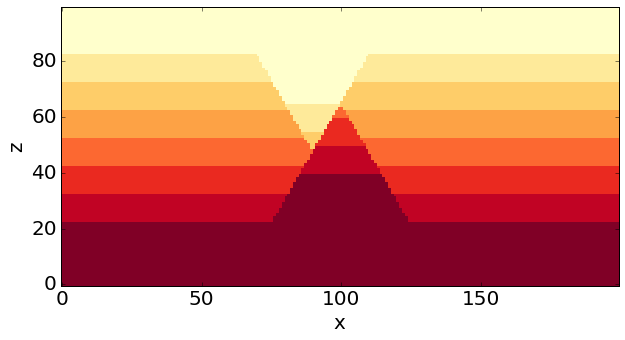
\includegraphics{4-Create-model_26_0.png}


\chapter{Read and Visualise Geophysical Potential-Fields}
\label{notebooks/5-Geophysical-Potential-Fields::doc}\label{notebooks/5-Geophysical-Potential-Fields:read-and-visualise-geophysical-potential-fields}
Geophysical potential fields (gravity and magnetics) can be calculated
directly from the generated kinematic model. A wide range of options
also exists to consider effects of geological events on the relevant
rock properties. We will here use pynoddy to simply and quickly test the
effect of changing geological structures on the calculated geophysical
response.

\begin{Verbatim}[commandchars=\\\{\}]
\PYGZpc{}matplotlib inline
\end{Verbatim}

\begin{Verbatim}[commandchars=\\\{\}]
\PYG{k+kn}{import} \PYG{n+nn}{sys}\PYG{o}{,} \PYG{n+nn}{os}
\PYG{k+kn}{import} \PYG{n+nn}{matplotlib.pyplot} \PYG{k+kn}{as} \PYG{n+nn}{plt}
\PYG{c}{\PYGZsh{} adjust some settings for matplotlib}
\PYG{k+kn}{from} \PYG{n+nn}{matplotlib} \PYG{k+kn}{import} \PYG{n}{rcParams}
\PYG{c}{\PYGZsh{} print rcParams}
\PYG{n}{rcParams}\PYG{p}{[}\PYG{l+s}{\PYGZsq{}}\PYG{l+s}{font.size}\PYG{l+s}{\PYGZsq{}}\PYG{p}{]} \PYG{o}{=} \PYG{l+m+mi}{15}
\PYG{c}{\PYGZsh{} determine path of repository to set paths corretly below}
\PYG{n}{repo\PYGZus{}path} \PYG{o}{=} \PYG{n}{os}\PYG{o}{.}\PYG{n}{path}\PYG{o}{.}\PYG{n}{realpath}\PYG{p}{(}\PYG{l+s}{\PYGZsq{}}\PYG{l+s}{../..}\PYG{l+s}{\PYGZsq{}}\PYG{p}{)}
\PYG{k+kn}{import} \PYG{n+nn}{pynoddy}
\end{Verbatim}

\begin{Verbatim}[commandchars=\\\{\}]
\PYG{k+kn}{import} \PYG{n+nn}{matplotlib.pyplot} \PYG{k+kn}{as} \PYG{n+nn}{plt}
\PYG{k+kn}{import} \PYG{n+nn}{numpy} \PYG{k+kn}{as} \PYG{n+nn}{np}
\end{Verbatim}

\begin{Verbatim}[commandchars=\\\{\}]
\PYG{k+kn}{from} \PYG{n+nn}{IPython.core.display} \PYG{k+kn}{import} \PYG{n}{HTML}
\PYG{n}{css\PYGZus{}file} \PYG{o}{=} \PYG{l+s}{\PYGZsq{}}\PYG{l+s}{pynoddy.css}\PYG{l+s}{\PYGZsq{}}
\PYG{n}{HTML}\PYG{p}{(}\PYG{n+nb}{open}\PYG{p}{(}\PYG{n}{css\PYGZus{}file}\PYG{p}{,} \PYG{l+s}{\PYGZdq{}}\PYG{l+s}{r}\PYG{l+s}{\PYGZdq{}}\PYG{p}{)}\PYG{o}{.}\PYG{n}{read}\PYG{p}{(}\PYG{p}{)}\PYG{p}{)}
\end{Verbatim}


\section{Read history file from Virtual Explorer}
\label{notebooks/5-Geophysical-Potential-Fields:read-history-file-from-virtual-explorer}
Many Noddy models are available on the site of the Virtual Explorer in
the Structural Geophysics Atlas. We will download and use one of these
models here as the base model.

We start with the history file of a ``Fold and Thrust Belt'' setting
stored on:

\code{http://tectonique.net/asg/ch3/ch3\_5/his/fold\_thrust.his}

The file can directly be downloaded and opened with pynoddy:

\begin{Verbatim}[commandchars=\\\{\}]
\PYG{k+kn}{import} \PYG{n+nn}{pynoddy.history}
\PYG{n+nb}{reload}\PYG{p}{(}\PYG{n}{pynoddy}\PYG{o}{.}\PYG{n}{history}\PYG{p}{)}

\PYG{n}{his} \PYG{o}{=} \PYG{n}{pynoddy}\PYG{o}{.}\PYG{n}{history}\PYG{o}{.}\PYG{n}{NoddyHistory}\PYG{p}{(}\PYG{n}{url} \PYG{o}{=} \PYGZbs{}
            \PYG{l+s}{\PYGZdq{}}\PYG{l+s}{http://tectonique.net/asg/ch3/ch3\PYGZus{}5/his/fold\PYGZus{}thrust.his}\PYG{l+s}{\PYGZdq{}}\PYG{p}{)}

\PYG{n}{his}\PYG{o}{.}\PYG{n}{determine\PYGZus{}model\PYGZus{}stratigraphy}\PYG{p}{(}\PYG{p}{)}
\end{Verbatim}

\begin{Verbatim}[commandchars=\\\{\}]
\PYG{n}{his}\PYG{o}{.}\PYG{n}{change\PYGZus{}cube\PYGZus{}size}\PYG{p}{(}\PYG{l+m+mi}{50}\PYG{p}{)}
\end{Verbatim}

\begin{Verbatim}[commandchars=\\\{\}]
\PYG{c}{\PYGZsh{} Save to (local) file to compute and visualise model}
\PYG{n}{history\PYGZus{}name} \PYG{o}{=} \PYG{l+s}{\PYGZdq{}}\PYG{l+s}{fold\PYGZus{}thrust.his}\PYG{l+s}{\PYGZdq{}}
\PYG{n}{his}\PYG{o}{.}\PYG{n}{write\PYGZus{}history}\PYG{p}{(}\PYG{n}{history\PYGZus{}name}\PYG{p}{)}
\PYG{c}{\PYGZsh{} his = pynoddy.history.NoddyHistory(history\PYGZus{}name)}
\end{Verbatim}

\begin{Verbatim}[commandchars=\\\{\}]
\PYG{n}{output} \PYG{o}{=} \PYG{l+s}{\PYGZdq{}}\PYG{l+s}{fold\PYGZus{}thrust\PYGZus{}out}\PYG{l+s}{\PYGZdq{}}
\PYG{n}{pynoddy}\PYG{o}{.}\PYG{n}{compute\PYGZus{}model}\PYG{p}{(}\PYG{n}{history\PYGZus{}name}\PYG{p}{,} \PYG{n}{output}\PYG{p}{)}
\end{Verbatim}

\begin{Verbatim}[commandchars=\\\{\}]
\PYG{l+s}{\PYGZsq{}}\PYG{l+s}{\PYGZsq{}}
\end{Verbatim}

\begin{Verbatim}[commandchars=\\\{\}]
\PYG{k+kn}{import} \PYG{n+nn}{pynoddy.output}
\PYG{c}{\PYGZsh{} load and visualise model}
\PYG{n}{h\PYGZus{}out} \PYG{o}{=} \PYG{n}{pynoddy}\PYG{o}{.}\PYG{n}{output}\PYG{o}{.}\PYG{n}{NoddyOutput}\PYG{p}{(}\PYG{n}{output}\PYG{p}{)}
\end{Verbatim}

\begin{Verbatim}[commandchars=\\\{\}]
\PYG{c}{\PYGZsh{} his.determine\PYGZus{}model\PYGZus{}stratigraphy()}
\PYG{n}{h\PYGZus{}out}\PYG{o}{.}\PYG{n}{plot\PYGZus{}section}\PYG{p}{(}\PYG{l+s}{\PYGZsq{}}\PYG{l+s}{x}\PYG{l+s}{\PYGZsq{}}\PYG{p}{,}
                   \PYG{n}{layer\PYGZus{}labels} \PYG{o}{=} \PYG{n}{his}\PYG{o}{.}\PYG{n}{model\PYGZus{}stratigraphy}\PYG{p}{,}
                   \PYG{n}{colorbar\PYGZus{}orientation} \PYG{o}{=} \PYG{l+s}{\PYGZsq{}}\PYG{l+s}{horizontal}\PYG{l+s}{\PYGZsq{}}\PYG{p}{,}
                   \PYG{n}{colorbar}\PYG{o}{=}\PYG{n+nb+bp}{False}\PYG{p}{,}
                   \PYG{n}{title} \PYG{o}{=} \PYG{l+s}{\PYGZsq{}}\PYG{l+s}{\PYGZsq{}}\PYG{p}{,}
\PYG{c}{\PYGZsh{}                   savefig=True, fig\PYGZus{}filename = \PYGZsq{}fold\PYGZus{}thrust\PYGZus{}NS\PYGZus{}section.eps\PYGZsq{},}
                   \PYG{n}{cmap} \PYG{o}{=} \PYG{l+s}{\PYGZsq{}}\PYG{l+s}{YlOrRd}\PYG{l+s}{\PYGZsq{}}\PYG{p}{)}
\end{Verbatim}

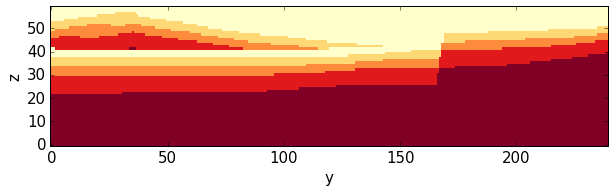
\includegraphics{5-Geophysical-Potential-Fields_11_0.png}

\begin{Verbatim}[commandchars=\\\{\}]
\PYG{n}{h\PYGZus{}out}\PYG{o}{.}\PYG{n}{plot\PYGZus{}section}\PYG{p}{(}\PYG{l+s}{\PYGZsq{}}\PYG{l+s}{y}\PYG{l+s}{\PYGZsq{}}\PYG{p}{,} \PYG{n}{layer\PYGZus{}labels} \PYG{o}{=} \PYG{n}{his}\PYG{o}{.}\PYG{n}{model\PYGZus{}stratigraphy}\PYG{p}{,}
                   \PYG{n}{colorbar\PYGZus{}orientation} \PYG{o}{=} \PYG{l+s}{\PYGZsq{}}\PYG{l+s}{horizontal}\PYG{l+s}{\PYGZsq{}}\PYG{p}{,} \PYG{n}{title} \PYG{o}{=} \PYG{l+s}{\PYGZsq{}}\PYG{l+s}{\PYGZsq{}}\PYG{p}{,} \PYG{n}{cmap} \PYG{o}{=} \PYG{l+s}{\PYGZsq{}}\PYG{l+s}{YlOrRd}\PYG{l+s}{\PYGZsq{}}\PYG{p}{,}
\PYG{c}{\PYGZsh{}                   savefig=True, fig\PYGZus{}filename = \PYGZsq{}fold\PYGZus{}thrust\PYGZus{}EW\PYGZus{}section.eps\PYGZsq{},}
                   \PYG{n}{ve}\PYG{o}{=}\PYG{l+m+mf}{1.5}\PYG{p}{)}
\end{Verbatim}

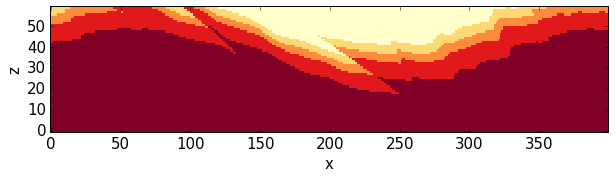
\includegraphics{5-Geophysical-Potential-Fields_12_0.png}

\begin{Verbatim}[commandchars=\\\{\}]
\PYG{n}{h\PYGZus{}out}\PYG{o}{.}\PYG{n}{export\PYGZus{}to\PYGZus{}vtk}\PYG{p}{(}\PYG{n}{vtk\PYGZus{}filename} \PYG{o}{=} \PYG{l+s}{\PYGZdq{}}\PYG{l+s}{fold\PYGZus{}thrust}\PYG{l+s}{\PYGZdq{}}\PYG{p}{)}
\end{Verbatim}


\section{Visualise calculated geophysical fields}
\label{notebooks/5-Geophysical-Potential-Fields:visualise-calculated-geophysical-fields}
The first step is to recompute the model with the generation of the
geophysical responses

\begin{Verbatim}[commandchars=\\\{\}]
\PYG{n}{pynoddy}\PYG{o}{.}\PYG{n}{compute\PYGZus{}model}\PYG{p}{(}\PYG{n}{history\PYGZus{}name}\PYG{p}{,} \PYG{n}{output}\PYG{p}{,} \PYG{n}{sim\PYGZus{}type} \PYG{o}{=} \PYG{l+s}{\PYGZsq{}}\PYG{l+s}{GEOPHYSICS}\PYG{l+s}{\PYGZsq{}}\PYG{p}{)}
\end{Verbatim}

\begin{Verbatim}[commandchars=\\\{\}]
\PYG{l+s}{\PYGZsq{}}\PYG{l+s}{\PYGZsq{}}
\end{Verbatim}

We now get two files for the caluclated fields: `.grv' for gravity, and
`.mag' for the magnetic field. We can extract the information of these
files for visualisation and further processing in python:

\begin{Verbatim}[commandchars=\\\{\}]
\PYG{n+nb}{reload}\PYG{p}{(}\PYG{n}{pynoddy}\PYG{o}{.}\PYG{n}{output}\PYG{p}{)}
\PYG{n}{geophys} \PYG{o}{=} \PYG{n}{pynoddy}\PYG{o}{.}\PYG{n}{output}\PYG{o}{.}\PYG{n}{NoddyGeophysics}\PYG{p}{(}\PYG{n}{output}\PYG{p}{)}
\end{Verbatim}

\begin{Verbatim}[commandchars=\\\{\}]
\PYG{n}{fig} \PYG{o}{=} \PYG{n}{plt}\PYG{o}{.}\PYG{n}{figure}\PYG{p}{(}\PYG{n}{figsize} \PYG{o}{=} \PYG{p}{(}\PYG{l+m+mi}{5}\PYG{p}{,}\PYG{l+m+mi}{5}\PYG{p}{)}\PYG{p}{)}
\PYG{n}{ax} \PYG{o}{=} \PYG{n}{fig}\PYG{o}{.}\PYG{n}{add\PYGZus{}subplot}\PYG{p}{(}\PYG{l+m+mi}{111}\PYG{p}{)}
\PYG{c}{\PYGZsh{} imshow(geophys.grv\PYGZus{}data, cmap = \PYGZsq{}jet\PYGZsq{})}
\PYG{c}{\PYGZsh{} define contour levels}
\PYG{n}{levels} \PYG{o}{=} \PYG{n}{np}\PYG{o}{.}\PYG{n}{arange}\PYG{p}{(}\PYG{l+m+mi}{322}\PYG{p}{,}\PYG{l+m+mi}{344}\PYG{p}{,}\PYG{l+m+mi}{1}\PYG{p}{)}
\PYG{n}{cf} \PYG{o}{=} \PYG{n}{ax}\PYG{o}{.}\PYG{n}{contourf}\PYG{p}{(}\PYG{n}{geophys}\PYG{o}{.}\PYG{n}{grv\PYGZus{}data}\PYG{p}{,} \PYG{n}{levels}\PYG{p}{,} \PYG{n}{cmap} \PYG{o}{=} \PYG{l+s}{\PYGZsq{}}\PYG{l+s}{gray}\PYG{l+s}{\PYGZsq{}}\PYG{p}{,} \PYG{n}{vmin} \PYG{o}{=} \PYG{l+m+mi}{324}\PYG{p}{,} \PYG{n}{vmax} \PYG{o}{=} \PYG{l+m+mi}{342}\PYG{p}{)}
\PYG{n}{cbar} \PYG{o}{=} \PYG{n}{plt}\PYG{o}{.}\PYG{n}{colorbar}\PYG{p}{(}\PYG{n}{cf}\PYG{p}{,} \PYG{n}{orientation} \PYG{o}{=} \PYG{l+s}{\PYGZsq{}}\PYG{l+s}{horizontal}\PYG{l+s}{\PYGZsq{}}\PYG{p}{)}
\PYG{c}{\PYGZsh{} print levels}
\end{Verbatim}

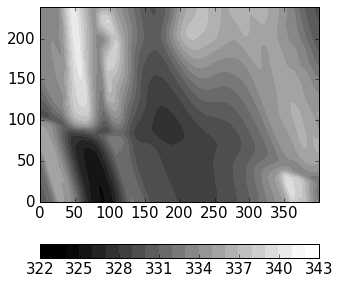
\includegraphics{5-Geophysical-Potential-Fields_18_0.png}


\section{Change history and compare gravity}
\label{notebooks/5-Geophysical-Potential-Fields:change-history-and-compare-gravity}
As a next step, we will now change aspects of the geological history
(paramtereised in as parameters of the kinematic events) and calculate
the effect on the gravity. Then, we will compare the changed gravity
field to the original field.

Let's have a look at the properties of the defined faults in the
original model:

\begin{Verbatim}[commandchars=\\\{\}]
\PYG{k}{for} \PYG{n}{i} \PYG{o+ow}{in} \PYG{n+nb}{range}\PYG{p}{(}\PYG{l+m+mi}{4}\PYG{p}{)}\PYG{p}{:}
    \PYG{k}{print}\PYG{p}{(}\PYG{l+s}{\PYGZdq{}}\PYG{l+s+se}{\PYGZbs{}n}\PYG{l+s}{Event }\PYG{l+s+si}{\PYGZpc{}d}\PYG{l+s}{\PYGZdq{}} \PYG{o}{\PYGZpc{}} \PYG{p}{(}\PYG{n}{i}\PYG{o}{+}\PYG{l+m+mi}{2}\PYG{p}{)}\PYG{p}{)}
    \PYG{k}{print} \PYG{l+s}{\PYGZdq{}}\PYG{l+s}{Event type:}\PYG{l+s+se}{\PYGZbs{}t}\PYG{l+s}{\PYGZdq{}} \PYG{o}{+} \PYG{n}{his}\PYG{o}{.}\PYG{n}{events}\PYG{p}{[}\PYG{n}{i}\PYG{o}{+}\PYG{l+m+mi}{2}\PYG{p}{]}\PYG{o}{.}\PYG{n}{event\PYGZus{}type}
    \PYG{k}{print} \PYG{l+s}{\PYGZdq{}}\PYG{l+s}{Fault slip:}\PYG{l+s+se}{\PYGZbs{}t}\PYG{l+s+si}{\PYGZpc{}.1f}\PYG{l+s}{\PYGZdq{}} \PYG{o}{\PYGZpc{}} \PYG{n}{his}\PYG{o}{.}\PYG{n}{events}\PYG{p}{[}\PYG{n}{i}\PYG{o}{+}\PYG{l+m+mi}{2}\PYG{p}{]}\PYG{o}{.}\PYG{n}{properties}\PYG{p}{[}\PYG{l+s}{\PYGZsq{}}\PYG{l+s}{Slip}\PYG{l+s}{\PYGZsq{}}\PYG{p}{]}
    \PYG{k}{print} \PYG{l+s}{\PYGZdq{}}\PYG{l+s}{Fault dip:}\PYG{l+s+se}{\PYGZbs{}t}\PYG{l+s+si}{\PYGZpc{}.1f}\PYG{l+s}{\PYGZdq{}} \PYG{o}{\PYGZpc{}} \PYG{n}{his}\PYG{o}{.}\PYG{n}{events}\PYG{p}{[}\PYG{n}{i}\PYG{o}{+}\PYG{l+m+mi}{2}\PYG{p}{]}\PYG{o}{.}\PYG{n}{properties}\PYG{p}{[}\PYG{l+s}{\PYGZsq{}}\PYG{l+s}{Dip}\PYG{l+s}{\PYGZsq{}}\PYG{p}{]}
    \PYG{k}{print} \PYG{l+s}{\PYGZdq{}}\PYG{l+s}{Dip direction:}\PYG{l+s+se}{\PYGZbs{}t}\PYG{l+s+si}{\PYGZpc{}.1f}\PYG{l+s}{\PYGZdq{}} \PYG{o}{\PYGZpc{}} \PYG{n}{his}\PYG{o}{.}\PYG{n}{events}\PYG{p}{[}\PYG{n}{i}\PYG{o}{+}\PYG{l+m+mi}{2}\PYG{p}{]}\PYG{o}{.}\PYG{n}{properties}\PYG{p}{[}\PYG{l+s}{\PYGZsq{}}\PYG{l+s}{Dip Direction}\PYG{l+s}{\PYGZsq{}}\PYG{p}{]}
\end{Verbatim}

\begin{Verbatim}[commandchars=\\\{\}]
Event 2
Event type: FAULT
Fault slip: \PYGZhy{}5000.0
Fault dip:  0.0
Dip direction:      90.0

Event 3
Event type: FAULT
Fault slip: \PYGZhy{}3000.0
Fault dip:  0.0
Dip direction:      90.0

Event 4
Event type: FAULT
Fault slip: \PYGZhy{}3000.0
Fault dip:  0.0
Dip direction:      90.0

Event 5
Event type: FAULT
Fault slip: 12000.0
Fault dip:  80.0
Dip direction:      170.0
\end{Verbatim}

\begin{Verbatim}[commandchars=\\\{\}]
\PYG{n+nb}{reload}\PYG{p}{(}\PYG{n}{pynoddy}\PYG{o}{.}\PYG{n}{history}\PYG{p}{)}
\PYG{n+nb}{reload}\PYG{p}{(}\PYG{n}{pynoddy}\PYG{o}{.}\PYG{n}{events}\PYG{p}{)}
\PYG{n}{his2} \PYG{o}{=} \PYG{n}{pynoddy}\PYG{o}{.}\PYG{n}{history}\PYG{o}{.}\PYG{n}{NoddyHistory}\PYG{p}{(}\PYG{l+s}{\PYGZdq{}}\PYG{l+s}{fold\PYGZus{}thrust.his}\PYG{l+s}{\PYGZdq{}}\PYG{p}{)}

\PYG{k}{print} \PYG{n}{his2}\PYG{o}{.}\PYG{n}{events}\PYG{p}{[}\PYG{l+m+mi}{6}\PYG{p}{]}\PYG{o}{.}\PYG{n}{properties}
\end{Verbatim}

\begin{Verbatim}[commandchars=\\\{\}]
\PYG{p}{\PYGZob{}}\PYG{l+s}{\PYGZsq{}}\PYG{l+s}{Dip}\PYG{l+s}{\PYGZsq{}}\PYG{p}{:} \PYG{l+m+mf}{130.0}\PYG{p}{,} \PYG{l+s}{\PYGZsq{}}\PYG{l+s}{Cylindricity}\PYG{l+s}{\PYGZsq{}}\PYG{p}{:} \PYG{l+m+mf}{0.0}\PYG{p}{,} \PYG{l+s}{\PYGZsq{}}\PYG{l+s}{Wavelength}\PYG{l+s}{\PYGZsq{}}\PYG{p}{:} \PYG{l+m+mf}{12000.0}\PYG{p}{,} \PYG{l+s}{\PYGZsq{}}\PYG{l+s}{Amplitude}\PYG{l+s}{\PYGZsq{}}\PYG{p}{:} \PYG{l+m+mf}{1000.0}\PYG{p}{,} \PYG{l+s}{\PYGZsq{}}\PYG{l+s}{Pitch}\PYG{l+s}{\PYGZsq{}}\PYG{p}{:} \PYG{l+m+mf}{0.0}\PYG{p}{,} \PYG{l+s}{\PYGZsq{}}\PYG{l+s}{Y}\PYG{l+s}{\PYGZsq{}}\PYG{p}{:} \PYG{l+m+mf}{0.0}\PYG{p}{,} \PYG{l+s}{\PYGZsq{}}\PYG{l+s}{X}\PYG{l+s}{\PYGZsq{}}\PYG{p}{:} \PYG{l+m+mf}{0.0}\PYG{p}{,} \PYG{l+s}{\PYGZsq{}}\PYG{l+s}{Single Fold}\PYG{l+s}{\PYGZsq{}}\PYG{p}{:} \PYG{l+s}{\PYGZsq{}}\PYG{l+s}{FALSE}\PYG{l+s}{\PYGZsq{}}\PYG{p}{,} \PYG{l+s}{\PYGZsq{}}\PYG{l+s}{Z}\PYG{l+s}{\PYGZsq{}}\PYG{p}{:} \PYG{l+m+mf}{0.0}\PYG{p}{,} \PYG{l+s}{\PYGZsq{}}\PYG{l+s}{Type}\PYG{l+s}{\PYGZsq{}}\PYG{p}{:} \PYG{l+s}{\PYGZsq{}}\PYG{l+s}{Fourier}\PYG{l+s}{\PYGZsq{}}\PYG{p}{,} \PYG{l+s}{\PYGZsq{}}\PYG{l+s}{Dip Direction}\PYG{l+s}{\PYGZsq{}}\PYG{p}{:} \PYG{l+m+mf}{110.0}\PYG{p}{\PYGZcb{}}
\end{Verbatim}

As a simple test, we are changing the fault slip for all the faults and
simply add 1000 m to all defined slips. In order to not mess up the
original model, we are creating a copy of the history object first:

\begin{Verbatim}[commandchars=\\\{\}]
\PYG{k+kn}{import} \PYG{n+nn}{copy}
\PYG{n}{his} \PYG{o}{=} \PYG{n}{pynoddy}\PYG{o}{.}\PYG{n}{history}\PYG{o}{.}\PYG{n}{NoddyHistory}\PYG{p}{(}\PYG{n}{history\PYGZus{}name}\PYG{p}{)}
\PYG{n}{his}\PYG{o}{.}\PYG{n}{all\PYGZus{}events\PYGZus{}end} \PYG{o}{+}\PYG{o}{=} \PYG{l+m+mi}{1}
\PYG{n}{his\PYGZus{}changed} \PYG{o}{=} \PYG{n}{copy}\PYG{o}{.}\PYG{n}{deepcopy}\PYG{p}{(}\PYG{n}{his}\PYG{p}{)}

\PYG{c}{\PYGZsh{} change parameters of kinematic events}
\PYG{n}{slip\PYGZus{}change} \PYG{o}{=} \PYG{l+m+mf}{2000.}
\PYG{n}{wavelength\PYGZus{}change} \PYG{o}{=} \PYG{l+m+mf}{2000.}
\PYG{c}{\PYGZsh{} his\PYGZus{}changed.events[3].properties[\PYGZsq{}Slip\PYGZsq{}] += slip\PYGZus{}change}
\PYG{c}{\PYGZsh{} his\PYGZus{}changed.events[5].properties[\PYGZsq{}Slip\PYGZsq{}] += slip\PYGZus{}change}
\PYG{c}{\PYGZsh{} change fold wavelength}
\PYG{n}{his\PYGZus{}changed}\PYG{o}{.}\PYG{n}{events}\PYG{p}{[}\PYG{l+m+mi}{6}\PYG{p}{]}\PYG{o}{.}\PYG{n}{properties}\PYG{p}{[}\PYG{l+s}{\PYGZsq{}}\PYG{l+s}{Wavelength}\PYG{l+s}{\PYGZsq{}}\PYG{p}{]} \PYG{o}{+}\PYG{o}{=} \PYG{n}{wavelength\PYGZus{}change}
\PYG{n}{his\PYGZus{}changed}\PYG{o}{.}\PYG{n}{events}\PYG{p}{[}\PYG{l+m+mi}{6}\PYG{p}{]}\PYG{o}{.}\PYG{n}{properties}\PYG{p}{[}\PYG{l+s}{\PYGZsq{}}\PYG{l+s}{X}\PYG{l+s}{\PYGZsq{}}\PYG{p}{]} \PYG{o}{+}\PYG{o}{=} \PYG{n}{wavelength\PYGZus{}change}\PYG{o}{/}\PYG{l+m+mf}{2.}
\end{Verbatim}

We now write the adjusted history back to a new history file and then
calculate the updated gravity field:

\begin{Verbatim}[commandchars=\\\{\}]
\PYG{n}{his\PYGZus{}changed}\PYG{o}{.}\PYG{n}{write\PYGZus{}history}\PYG{p}{(}\PYG{l+s}{\PYGZsq{}}\PYG{l+s}{fold\PYGZus{}thrust\PYGZus{}changed.his}\PYG{l+s}{\PYGZsq{}}\PYG{p}{)}
\end{Verbatim}

\begin{Verbatim}[commandchars=\\\{\}]
\PYG{c}{\PYGZsh{} \PYGZpc{}\PYGZpc{}timeit}
\PYG{c}{\PYGZsh{} recompute block model}
\PYG{n}{pynoddy}\PYG{o}{.}\PYG{n}{compute\PYGZus{}model}\PYG{p}{(}\PYG{l+s}{\PYGZsq{}}\PYG{l+s}{fold\PYGZus{}thrust\PYGZus{}changed.his}\PYG{l+s}{\PYGZsq{}}\PYG{p}{,} \PYG{l+s}{\PYGZsq{}}\PYG{l+s}{fold\PYGZus{}thrust\PYGZus{}changed\PYGZus{}out}\PYG{l+s}{\PYGZsq{}}\PYG{p}{)}
\end{Verbatim}

\begin{Verbatim}[commandchars=\\\{\}]
\PYG{l+s}{\PYGZsq{}}\PYG{l+s}{\PYGZsq{}}
\end{Verbatim}

\begin{Verbatim}[commandchars=\\\{\}]
\PYG{c}{\PYGZsh{} \PYGZpc{}\PYGZpc{}timeit}
\PYG{c}{\PYGZsh{} recompute geophysical response}
\PYG{n}{pynoddy}\PYG{o}{.}\PYG{n}{compute\PYGZus{}model}\PYG{p}{(}\PYG{l+s}{\PYGZsq{}}\PYG{l+s}{fold\PYGZus{}thrust\PYGZus{}changed.his}\PYG{l+s}{\PYGZsq{}}\PYG{p}{,} \PYG{l+s}{\PYGZsq{}}\PYG{l+s}{fold\PYGZus{}thrust\PYGZus{}changed\PYGZus{}out}\PYG{l+s}{\PYGZsq{}}\PYG{p}{,}
                      \PYG{n}{sim\PYGZus{}type} \PYG{o}{=} \PYG{l+s}{\PYGZsq{}}\PYG{l+s}{GEOPHYSICS}\PYG{l+s}{\PYGZsq{}}\PYG{p}{)}
\end{Verbatim}

\begin{Verbatim}[commandchars=\\\{\}]
\PYG{l+s}{\PYGZsq{}}\PYG{l+s}{\PYGZsq{}}
\end{Verbatim}

\begin{Verbatim}[commandchars=\\\{\}]
\PYG{c}{\PYGZsh{} load changed block model}
\PYG{n}{geo\PYGZus{}changed} \PYG{o}{=} \PYG{n}{pynoddy}\PYG{o}{.}\PYG{n}{output}\PYG{o}{.}\PYG{n}{NoddyOutput}\PYG{p}{(}\PYG{l+s}{\PYGZsq{}}\PYG{l+s}{fold\PYGZus{}thrust\PYGZus{}changed\PYGZus{}out}\PYG{l+s}{\PYGZsq{}}\PYG{p}{)}
\PYG{c}{\PYGZsh{} load output and visualise geophysical field}
\PYG{n}{geophys\PYGZus{}changed} \PYG{o}{=} \PYG{n}{pynoddy}\PYG{o}{.}\PYG{n}{output}\PYG{o}{.}\PYG{n}{NoddyGeophysics}\PYG{p}{(}\PYG{l+s}{\PYGZsq{}}\PYG{l+s}{fold\PYGZus{}thrust\PYGZus{}changed\PYGZus{}out}\PYG{l+s}{\PYGZsq{}}\PYG{p}{)}
\end{Verbatim}

\begin{Verbatim}[commandchars=\\\{\}]
\PYG{n}{fig} \PYG{o}{=} \PYG{n}{plt}\PYG{o}{.}\PYG{n}{figure}\PYG{p}{(}\PYG{n}{figsize} \PYG{o}{=} \PYG{p}{(}\PYG{l+m+mi}{5}\PYG{p}{,}\PYG{l+m+mi}{5}\PYG{p}{)}\PYG{p}{)}
\PYG{n}{ax} \PYG{o}{=} \PYG{n}{fig}\PYG{o}{.}\PYG{n}{add\PYGZus{}subplot}\PYG{p}{(}\PYG{l+m+mi}{111}\PYG{p}{)}
\PYG{c}{\PYGZsh{} imshow(geophys\PYGZus{}changed.grv\PYGZus{}data, cmap = \PYGZsq{}jet\PYGZsq{})}
\PYG{n}{cf} \PYG{o}{=} \PYG{n}{ax}\PYG{o}{.}\PYG{n}{contourf}\PYG{p}{(}\PYG{n}{geophys\PYGZus{}changed}\PYG{o}{.}\PYG{n}{grv\PYGZus{}data}\PYG{p}{,} \PYG{n}{levels}\PYG{p}{,} \PYG{n}{cmap} \PYG{o}{=} \PYG{l+s}{\PYGZsq{}}\PYG{l+s}{gray}\PYG{l+s}{\PYGZsq{}}\PYG{p}{,} \PYG{n}{vmin} \PYG{o}{=} \PYG{l+m+mi}{324}\PYG{p}{,} \PYG{n}{vmax} \PYG{o}{=} \PYG{l+m+mi}{342}\PYG{p}{)}
\PYG{n}{cbar} \PYG{o}{=} \PYG{n}{plt}\PYG{o}{.}\PYG{n}{colorbar}\PYG{p}{(}\PYG{n}{cf}\PYG{p}{,} \PYG{n}{orientation} \PYG{o}{=} \PYG{l+s}{\PYGZsq{}}\PYG{l+s}{horizontal}\PYG{l+s}{\PYGZsq{}}\PYG{p}{)}
\end{Verbatim}

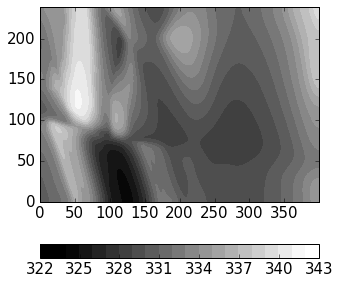
\includegraphics{5-Geophysical-Potential-Fields_30_0.png}

\begin{Verbatim}[commandchars=\\\{\}]
\PYG{n}{fig} \PYG{o}{=} \PYG{n}{plt}\PYG{o}{.}\PYG{n}{figure}\PYG{p}{(}\PYG{n}{figsize} \PYG{o}{=} \PYG{p}{(}\PYG{l+m+mi}{5}\PYG{p}{,}\PYG{l+m+mi}{5}\PYG{p}{)}\PYG{p}{)}
\PYG{n}{ax} \PYG{o}{=} \PYG{n}{fig}\PYG{o}{.}\PYG{n}{add\PYGZus{}subplot}\PYG{p}{(}\PYG{l+m+mi}{111}\PYG{p}{)}
\PYG{c}{\PYGZsh{} imshow(geophys.grv\PYGZus{}data \PYGZhy{} geophys\PYGZus{}changed.grv\PYGZus{}data, cmap = \PYGZsq{}jet\PYGZsq{})}
\PYG{n}{maxval} \PYG{o}{=} \PYG{n}{np}\PYG{o}{.}\PYG{n}{ceil}\PYG{p}{(}\PYG{n}{np}\PYG{o}{.}\PYG{n}{max}\PYG{p}{(}\PYG{n}{np}\PYG{o}{.}\PYG{n}{abs}\PYG{p}{(}\PYG{n}{geophys}\PYG{o}{.}\PYG{n}{grv\PYGZus{}data} \PYG{o}{\PYGZhy{}} \PYG{n}{geophys\PYGZus{}changed}\PYG{o}{.}\PYG{n}{grv\PYGZus{}data}\PYG{p}{)}\PYG{p}{)}\PYG{p}{)}
\PYG{c}{\PYGZsh{} comp\PYGZus{}levels = np.arange(\PYGZhy{}maxval,1.01 * maxval, 0.05 * maxval)}
\PYG{n}{cf} \PYG{o}{=} \PYG{n}{ax}\PYG{o}{.}\PYG{n}{contourf}\PYG{p}{(}\PYG{n}{geophys}\PYG{o}{.}\PYG{n}{grv\PYGZus{}data} \PYG{o}{\PYGZhy{}} \PYG{n}{geophys\PYGZus{}changed}\PYG{o}{.}\PYG{n}{grv\PYGZus{}data}\PYG{p}{,} \PYG{l+m+mi}{20}\PYG{p}{,}
                 \PYG{n}{cmap} \PYG{o}{=} \PYG{l+s}{\PYGZsq{}}\PYG{l+s}{spectral}\PYG{l+s}{\PYGZsq{}}\PYG{p}{)}
\PYG{n}{cbar} \PYG{o}{=} \PYG{n}{plt}\PYG{o}{.}\PYG{n}{colorbar}\PYG{p}{(}\PYG{n}{cf}\PYG{p}{,} \PYG{n}{orientation} \PYG{o}{=} \PYG{l+s}{\PYGZsq{}}\PYG{l+s}{horizontal}\PYG{l+s}{\PYGZsq{}}\PYG{p}{)}
\end{Verbatim}

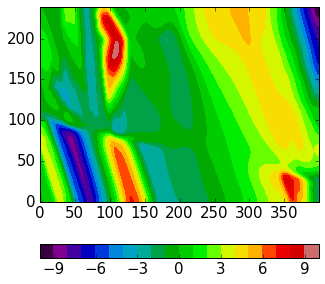
\includegraphics{5-Geophysical-Potential-Fields_31_0.png}

\begin{Verbatim}[commandchars=\\\{\}]
\PYG{c}{\PYGZsh{} compare sections through model}
\PYG{n}{geo\PYGZus{}changed}\PYG{o}{.}\PYG{n}{plot\PYGZus{}section}\PYG{p}{(}\PYG{l+s}{\PYGZsq{}}\PYG{l+s}{y}\PYG{l+s}{\PYGZsq{}}\PYG{p}{,} \PYG{n}{colorbar} \PYG{o}{=} \PYG{n+nb+bp}{False}\PYG{p}{)}
\PYG{n}{h\PYGZus{}out}\PYG{o}{.}\PYG{n}{plot\PYGZus{}section}\PYG{p}{(}\PYG{l+s}{\PYGZsq{}}\PYG{l+s}{y}\PYG{l+s}{\PYGZsq{}}\PYG{p}{,} \PYG{n}{colorbar} \PYG{o}{=} \PYG{n+nb+bp}{False}\PYG{p}{)}
\end{Verbatim}

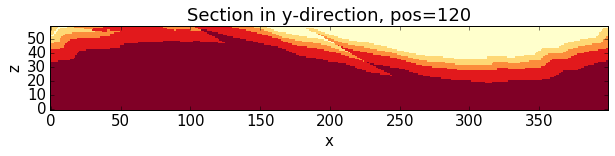
\includegraphics{5-Geophysical-Potential-Fields_32_0.png}

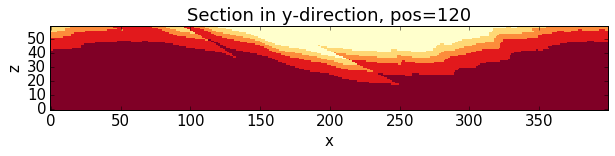
\includegraphics{5-Geophysical-Potential-Fields_32_1.png}

\begin{Verbatim}[commandchars=\\\{\}]
\PYG{k}{for} \PYG{n}{i} \PYG{o+ow}{in} \PYG{n+nb}{range}\PYG{p}{(}\PYG{l+m+mi}{4}\PYG{p}{)}\PYG{p}{:}
    \PYG{k}{print}\PYG{p}{(}\PYG{l+s}{\PYGZdq{}}\PYG{l+s}{Event }\PYG{l+s+si}{\PYGZpc{}d}\PYG{l+s}{\PYGZdq{}} \PYG{o}{\PYGZpc{}} \PYG{p}{(}\PYG{n}{i}\PYG{o}{+}\PYG{l+m+mi}{2}\PYG{p}{)}\PYG{p}{)}
    \PYG{k}{print} \PYG{n}{his}\PYG{o}{.}\PYG{n}{events}\PYG{p}{[}\PYG{n}{i}\PYG{o}{+}\PYG{l+m+mi}{2}\PYG{p}{]}\PYG{o}{.}\PYG{n}{properties}\PYG{p}{[}\PYG{l+s}{\PYGZsq{}}\PYG{l+s}{Slip}\PYG{l+s}{\PYGZsq{}}\PYG{p}{]}
    \PYG{k}{print} \PYG{n}{his}\PYG{o}{.}\PYG{n}{events}\PYG{p}{[}\PYG{n}{i}\PYG{o}{+}\PYG{l+m+mi}{2}\PYG{p}{]}\PYG{o}{.}\PYG{n}{properties}\PYG{p}{[}\PYG{l+s}{\PYGZsq{}}\PYG{l+s}{Dip}\PYG{l+s}{\PYGZsq{}}\PYG{p}{]}
    \PYG{k}{print} \PYG{n}{his}\PYG{o}{.}\PYG{n}{events}\PYG{p}{[}\PYG{n}{i}\PYG{o}{+}\PYG{l+m+mi}{2}\PYG{p}{]}\PYG{o}{.}\PYG{n}{properties}\PYG{p}{[}\PYG{l+s}{\PYGZsq{}}\PYG{l+s}{Dip Direction}\PYG{l+s}{\PYGZsq{}}\PYG{p}{]}
\end{Verbatim}

\begin{Verbatim}[commandchars=\\\{\}]
Event 2
\PYGZhy{}5000.0
0.0
90.0
Event 3
\PYGZhy{}3000.0
0.0
90.0
Event 4
\PYGZhy{}3000.0
0.0
90.0
Event 5
12000.0
80.0
170.0
\end{Verbatim}

\begin{Verbatim}[commandchars=\\\{\}]
\PYG{c}{\PYGZsh{} recompute the geology blocks for comparison:}
\PYG{n}{pynoddy}\PYG{o}{.}\PYG{n}{compute\PYGZus{}model}\PYG{p}{(}\PYG{l+s}{\PYGZsq{}}\PYG{l+s}{fold\PYGZus{}thrust\PYGZus{}changed.his}\PYG{l+s}{\PYGZsq{}}\PYG{p}{,} \PYG{l+s}{\PYGZsq{}}\PYG{l+s}{fold\PYGZus{}thrust\PYGZus{}changed\PYGZus{}out}\PYG{l+s}{\PYGZsq{}}\PYG{p}{)}
\end{Verbatim}

\begin{Verbatim}[commandchars=\\\{\}]
\PYG{l+s}{\PYGZsq{}}\PYG{l+s}{\PYGZsq{}}
\end{Verbatim}

\begin{Verbatim}[commandchars=\\\{\}]
\PYG{n}{geology\PYGZus{}changed} \PYG{o}{=} \PYG{n}{pynoddy}\PYG{o}{.}\PYG{n}{output}\PYG{o}{.}\PYG{n}{NoddyOutput}\PYG{p}{(}\PYG{l+s}{\PYGZsq{}}\PYG{l+s}{fold\PYGZus{}thrust\PYGZus{}changed\PYGZus{}out}\PYG{l+s}{\PYGZsq{}}\PYG{p}{)}
\end{Verbatim}

\begin{Verbatim}[commandchars=\\\{\}]
\PYG{n}{geology\PYGZus{}changed}\PYG{o}{.}\PYG{n}{plot\PYGZus{}section}\PYG{p}{(}\PYG{l+s}{\PYGZsq{}}\PYG{l+s}{x}\PYG{l+s}{\PYGZsq{}}\PYG{p}{,}
\PYG{c}{\PYGZsh{}                    layer\PYGZus{}labels = his.model\PYGZus{}stratigraphy,}
                   \PYG{n}{colorbar\PYGZus{}orientation} \PYG{o}{=} \PYG{l+s}{\PYGZsq{}}\PYG{l+s}{horizontal}\PYG{l+s}{\PYGZsq{}}\PYG{p}{,}
                   \PYG{n}{colorbar}\PYG{o}{=}\PYG{n+nb+bp}{False}\PYG{p}{,}
                   \PYG{n}{title} \PYG{o}{=} \PYG{l+s}{\PYGZsq{}}\PYG{l+s}{\PYGZsq{}}\PYG{p}{,}
\PYG{c}{\PYGZsh{}                   savefig=True, fig\PYGZus{}filename = \PYGZsq{}fold\PYGZus{}thrust\PYGZus{}NS\PYGZus{}section.eps\PYGZsq{},}
                   \PYG{n}{cmap} \PYG{o}{=} \PYG{l+s}{\PYGZsq{}}\PYG{l+s}{YlOrRd}\PYG{l+s}{\PYGZsq{}}\PYG{p}{)}
\end{Verbatim}

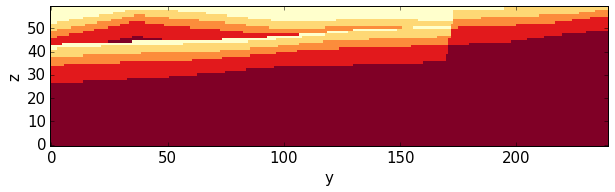
\includegraphics{5-Geophysical-Potential-Fields_36_0.png}

\begin{Verbatim}[commandchars=\\\{\}]
\PYG{n}{geology\PYGZus{}changed}\PYG{o}{.}\PYG{n}{plot\PYGZus{}section}\PYG{p}{(}\PYG{l+s}{\PYGZsq{}}\PYG{l+s}{y}\PYG{l+s}{\PYGZsq{}}\PYG{p}{,}
                             \PYG{c}{\PYGZsh{} layer\PYGZus{}labels = his.model\PYGZus{}stratigraphy,}
                   \PYG{n}{colorbar\PYGZus{}orientation} \PYG{o}{=} \PYG{l+s}{\PYGZsq{}}\PYG{l+s}{horizontal}\PYG{l+s}{\PYGZsq{}}\PYG{p}{,} \PYG{n}{title} \PYG{o}{=} \PYG{l+s}{\PYGZsq{}}\PYG{l+s}{\PYGZsq{}}\PYG{p}{,} \PYG{n}{cmap} \PYG{o}{=} \PYG{l+s}{\PYGZsq{}}\PYG{l+s}{YlOrRd}\PYG{l+s}{\PYGZsq{}}\PYG{p}{,}
\PYG{c}{\PYGZsh{}                   savefig=True, fig\PYGZus{}filename = \PYGZsq{}fold\PYGZus{}thrust\PYGZus{}EW\PYGZus{}section.eps\PYGZsq{},}
                   \PYG{n}{ve}\PYG{o}{=}\PYG{l+m+mf}{1.5}\PYG{p}{)}
\end{Verbatim}

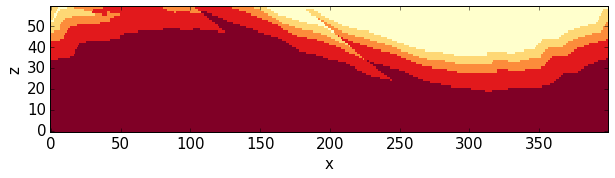
\includegraphics{5-Geophysical-Potential-Fields_37_0.png}

\begin{Verbatim}[commandchars=\\\{\}]
\PYG{c}{\PYGZsh{} Calculate block difference and export as VTK for 3\PYGZhy{}D visualisation:}
\PYG{k+kn}{import} \PYG{n+nn}{copy}
\PYG{n}{diff\PYGZus{}model} \PYG{o}{=} \PYG{n}{copy}\PYG{o}{.}\PYG{n}{deepcopy}\PYG{p}{(}\PYG{n}{geology\PYGZus{}changed}\PYG{p}{)}
\PYG{n}{diff\PYGZus{}model}\PYG{o}{.}\PYG{n}{block} \PYG{o}{\PYGZhy{}}\PYG{o}{=} \PYG{n}{h\PYGZus{}out}\PYG{o}{.}\PYG{n}{block}
\end{Verbatim}

\begin{Verbatim}[commandchars=\\\{\}]
\PYG{n}{diff\PYGZus{}model}\PYG{o}{.}\PYG{n}{export\PYGZus{}to\PYGZus{}vtk}\PYG{p}{(}\PYG{n}{vtk\PYGZus{}filename} \PYG{o}{=} \PYG{l+s}{\PYGZdq{}}\PYG{l+s}{diff\PYGZus{}model\PYGZus{}fold\PYGZus{}thrust\PYGZus{}belt}\PYG{l+s}{\PYGZdq{}}\PYG{p}{)}
\end{Verbatim}


\section{Figure with all results}
\label{notebooks/5-Geophysical-Potential-Fields:figure-with-all-results}
We now create a figure with the gravity field of the original and the
changed model, as well as a difference plot to highlight areas with
significant changes. This example also shows how additional equations
can easily be combined with pynoddy classes.

\begin{Verbatim}[commandchars=\\\{\}]
\PYG{n}{fig} \PYG{o}{=} \PYG{n}{plt}\PYG{o}{.}\PYG{n}{figure}\PYG{p}{(}\PYG{n}{figsize}\PYG{o}{=}\PYG{p}{(}\PYG{l+m+mi}{20}\PYG{p}{,}\PYG{l+m+mi}{8}\PYG{p}{)}\PYG{p}{)}
\PYG{n}{ax1} \PYG{o}{=} \PYG{n}{fig}\PYG{o}{.}\PYG{n}{add\PYGZus{}subplot}\PYG{p}{(}\PYG{l+m+mi}{131}\PYG{p}{)}
\PYG{c}{\PYGZsh{} original plot}
\PYG{n}{levels} \PYG{o}{=} \PYG{n}{np}\PYG{o}{.}\PYG{n}{arange}\PYG{p}{(}\PYG{l+m+mi}{322}\PYG{p}{,}\PYG{l+m+mi}{344}\PYG{p}{,}\PYG{l+m+mi}{1}\PYG{p}{)}
\PYG{n}{cf1} \PYG{o}{=} \PYG{n}{ax1}\PYG{o}{.}\PYG{n}{contourf}\PYG{p}{(}\PYG{n}{geophys}\PYG{o}{.}\PYG{n}{grv\PYGZus{}data}\PYG{p}{,} \PYG{n}{levels}\PYG{p}{,} \PYG{n}{cmap} \PYG{o}{=} \PYG{l+s}{\PYGZsq{}}\PYG{l+s}{gray}\PYG{l+s}{\PYGZsq{}}\PYG{p}{,} \PYG{n}{vmin} \PYG{o}{=} \PYG{l+m+mi}{324}\PYG{p}{,} \PYG{n}{vmax} \PYG{o}{=} \PYG{l+m+mi}{342}\PYG{p}{)}
\PYG{c}{\PYGZsh{} cbar1 = ax1.colorbar(cf1, orientation = \PYGZsq{}horizontal\PYGZsq{})}
\PYG{n}{fig}\PYG{o}{.}\PYG{n}{colorbar}\PYG{p}{(}\PYG{n}{cf1}\PYG{p}{,} \PYG{n}{orientation}\PYG{o}{=}\PYG{l+s}{\PYGZsq{}}\PYG{l+s}{horizontal}\PYG{l+s}{\PYGZsq{}}\PYG{p}{)}
\PYG{n}{ax1}\PYG{o}{.}\PYG{n}{set\PYGZus{}title}\PYG{p}{(}\PYG{l+s}{\PYGZsq{}}\PYG{l+s}{Gravity of original model}\PYG{l+s}{\PYGZsq{}}\PYG{p}{)}

\PYG{n}{ax2} \PYG{o}{=} \PYG{n}{fig}\PYG{o}{.}\PYG{n}{add\PYGZus{}subplot}\PYG{p}{(}\PYG{l+m+mi}{132}\PYG{p}{)}




\PYG{n}{cf2} \PYG{o}{=} \PYG{n}{ax2}\PYG{o}{.}\PYG{n}{contourf}\PYG{p}{(}\PYG{n}{geophys\PYGZus{}changed}\PYG{o}{.}\PYG{n}{grv\PYGZus{}data}\PYG{p}{,} \PYG{n}{levels}\PYG{p}{,} \PYG{n}{cmap} \PYG{o}{=} \PYG{l+s}{\PYGZsq{}}\PYG{l+s}{gray}\PYG{l+s}{\PYGZsq{}}\PYG{p}{,} \PYG{n}{vmin} \PYG{o}{=} \PYG{l+m+mi}{324}\PYG{p}{,} \PYG{n}{vmax} \PYG{o}{=} \PYG{l+m+mi}{342}\PYG{p}{)}
\PYG{n}{ax2}\PYG{o}{.}\PYG{n}{set\PYGZus{}title}\PYG{p}{(}\PYG{l+s}{\PYGZsq{}}\PYG{l+s}{Gravity of changed model}\PYG{l+s}{\PYGZsq{}}\PYG{p}{)}
\PYG{n}{fig}\PYG{o}{.}\PYG{n}{colorbar}\PYG{p}{(}\PYG{n}{cf2}\PYG{p}{,} \PYG{n}{orientation}\PYG{o}{=}\PYG{l+s}{\PYGZsq{}}\PYG{l+s}{horizontal}\PYG{l+s}{\PYGZsq{}}\PYG{p}{)}

\PYG{n}{ax3} \PYG{o}{=} \PYG{n}{fig}\PYG{o}{.}\PYG{n}{add\PYGZus{}subplot}\PYG{p}{(}\PYG{l+m+mi}{133}\PYG{p}{)}


\PYG{n}{comp\PYGZus{}levels} \PYG{o}{=} \PYG{n}{np}\PYG{o}{.}\PYG{n}{arange}\PYG{p}{(}\PYG{o}{\PYGZhy{}}\PYG{l+m+mf}{10.}\PYG{p}{,}\PYG{l+m+mf}{10.1}\PYG{p}{,}\PYG{l+m+mf}{0.25}\PYG{p}{)}
\PYG{n}{cf3} \PYG{o}{=} \PYG{n}{ax3}\PYG{o}{.}\PYG{n}{contourf}\PYG{p}{(}\PYG{n}{geophys}\PYG{o}{.}\PYG{n}{grv\PYGZus{}data} \PYG{o}{\PYGZhy{}} \PYG{n}{geophys\PYGZus{}changed}\PYG{o}{.}\PYG{n}{grv\PYGZus{}data}\PYG{p}{,} \PYG{n}{comp\PYGZus{}levels}\PYG{p}{,} \PYG{n}{cmap} \PYG{o}{=} \PYG{l+s}{\PYGZsq{}}\PYG{l+s}{RdBu\PYGZus{}r}\PYG{l+s}{\PYGZsq{}}\PYG{p}{)}
\PYG{n}{ax3}\PYG{o}{.}\PYG{n}{set\PYGZus{}title}\PYG{p}{(}\PYG{l+s}{\PYGZsq{}}\PYG{l+s}{Gravity difference}\PYG{l+s}{\PYGZsq{}}\PYG{p}{)}

\PYG{n}{fig}\PYG{o}{.}\PYG{n}{colorbar}\PYG{p}{(}\PYG{n}{cf3}\PYG{p}{,} \PYG{n}{orientation}\PYG{o}{=}\PYG{l+s}{\PYGZsq{}}\PYG{l+s}{horizontal}\PYG{l+s}{\PYGZsq{}}\PYG{p}{)}

\PYG{n}{plt}\PYG{o}{.}\PYG{n}{savefig}\PYG{p}{(}\PYG{l+s}{\PYGZdq{}}\PYG{l+s}{grav\PYGZus{}ori\PYGZus{}changed\PYGZus{}compared.eps}\PYG{l+s}{\PYGZdq{}}\PYG{p}{)}
\end{Verbatim}

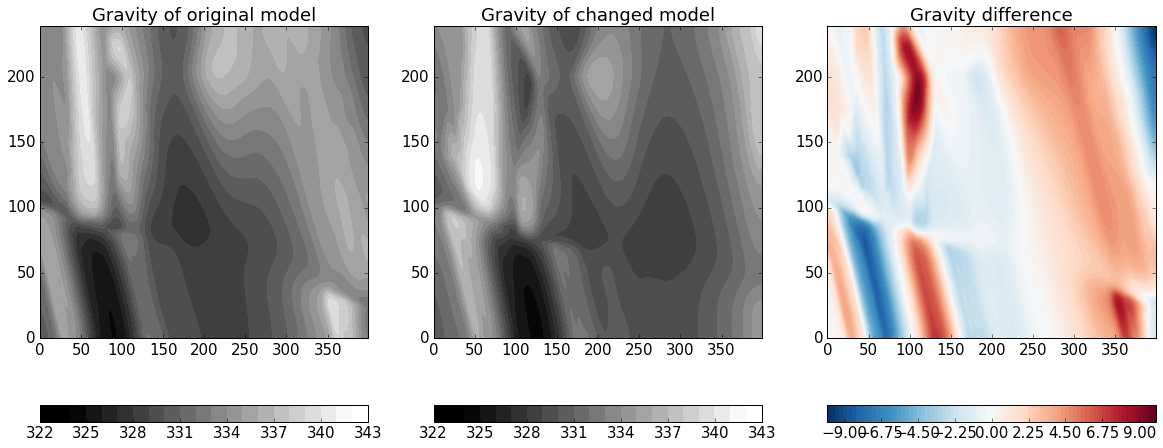
\includegraphics{5-Geophysical-Potential-Fields_41_0.png}


\chapter{Reproducible Experiments with pynoddy}
\label{notebooks/6-Reproducible-Experiments:reproducible-experiments-with-pynoddy}\label{notebooks/6-Reproducible-Experiments::doc}
All \code{pynoddy} experiments can be defined in a Python script, and if
all settings are appropriate, then this script can be re-run to obtain a
reproduction of the results. However, it is often more convenient to
encapsulate all elements of an experiment within one class. We show here
how this is done in the \code{pynoddy.experiment.Experiment} class and how
this class can be used to define simple reproducible experiments with
kinematic models.

\begin{Verbatim}[commandchars=\\\{\}]
\PYG{k+kn}{from} \PYG{n+nn}{IPython.core.display} \PYG{k+kn}{import} \PYG{n}{HTML}
\PYG{n}{css\PYGZus{}file} \PYG{o}{=} \PYG{l+s}{\PYGZsq{}}\PYG{l+s}{pynoddy.css}\PYG{l+s}{\PYGZsq{}}
\PYG{n}{HTML}\PYG{p}{(}\PYG{n+nb}{open}\PYG{p}{(}\PYG{n}{css\PYGZus{}file}\PYG{p}{,} \PYG{l+s}{\PYGZdq{}}\PYG{l+s}{r}\PYG{l+s}{\PYGZdq{}}\PYG{p}{)}\PYG{o}{.}\PYG{n}{read}\PYG{p}{(}\PYG{p}{)}\PYG{p}{)}
\end{Verbatim}

\begin{Verbatim}[commandchars=\\\{\}]
\PYGZpc{}matplotlib inline
\end{Verbatim}

\begin{Verbatim}[commandchars=\\\{\}]
\PYG{c}{\PYGZsh{} here the usual imports. If any of the imports fails,}
\PYG{c}{\PYGZsh{} make sure that pynoddy is installed}
\PYG{c}{\PYGZsh{} properly, ideally with \PYGZsq{}python setup.py develop\PYGZsq{}}
\PYG{c}{\PYGZsh{} or \PYGZsq{}python setup.py install\PYGZsq{}}
\PYG{k+kn}{import} \PYG{n+nn}{sys}\PYG{o}{,} \PYG{n+nn}{os}
\PYG{k+kn}{import} \PYG{n+nn}{matplotlib.pyplot} \PYG{k+kn}{as} \PYG{n+nn}{plt}
\PYG{k+kn}{import} \PYG{n+nn}{numpy} \PYG{k+kn}{as} \PYG{n+nn}{np}
\PYG{c}{\PYGZsh{} adjust some settings for matplotlib}
\PYG{k+kn}{from} \PYG{n+nn}{matplotlib} \PYG{k+kn}{import} \PYG{n}{rcParams}
\PYG{c}{\PYGZsh{} print rcParams}
\PYG{n}{rcParams}\PYG{p}{[}\PYG{l+s}{\PYGZsq{}}\PYG{l+s}{font.size}\PYG{l+s}{\PYGZsq{}}\PYG{p}{]} \PYG{o}{=} \PYG{l+m+mi}{15}
\PYG{c}{\PYGZsh{} determine path of repository to set paths corretly below}
\PYG{n}{repo\PYGZus{}path} \PYG{o}{=} \PYG{n}{os}\PYG{o}{.}\PYG{n}{path}\PYG{o}{.}\PYG{n}{realpath}\PYG{p}{(}\PYG{l+s}{\PYGZsq{}}\PYG{l+s}{../..}\PYG{l+s}{\PYGZsq{}}\PYG{p}{)}
\PYG{k+kn}{import} \PYG{n+nn}{pynoddy.history}
\PYG{k+kn}{import} \PYG{n+nn}{pynoddy.experiment}
\PYG{n+nb}{reload}\PYG{p}{(}\PYG{n}{pynoddy}\PYG{o}{.}\PYG{n}{experiment}\PYG{p}{)}
\PYG{n}{rcParams}\PYG{o}{.}\PYG{n}{update}\PYG{p}{(}\PYG{p}{\PYGZob{}}\PYG{l+s}{\PYGZsq{}}\PYG{l+s}{font.size}\PYG{l+s}{\PYGZsq{}}\PYG{p}{:} \PYG{l+m+mi}{15}\PYG{p}{\PYGZcb{}}\PYG{p}{)}
\end{Verbatim}


\section{Defining an experiment}
\label{notebooks/6-Reproducible-Experiments:defining-an-experiment}
We are considering the following scenario: we defined a kinematic model
of a prospective geological unit at depth. As we know that the estimates
of the (kinematic) model parameters contain a high degree of
uncertainty, we would like to represent this uncertainty with the model.

Our approach is here to perform a randomised uncertainty propagation
analysis with a Monte Carlo sampling method. Results should be presented
in several figures (2-D slice plots and a VTK representation in 3-D).

To perform this analysis, we need to perform the following steps (see
main paper for more details):
\begin{enumerate}
\item {} 
Define kinematic model parameters and construct the initial (base)
model;

\item {} 
Assign probability distributions (and possible parameter
correlations) to relevant uncertain input parameters;

\item {} 
Generate a set of n random realisations, repeating the following
steps:
\begin{enumerate}
\item {} 
Draw a randomised input parameter set from the parameter distribu-
tion;

\item {} 
Generate a model with this parameter set;

\item {} 
Analyse the generated model and store results;

\end{enumerate}

\item {} 
Finally: perform postprocessing, generate figures of results

\end{enumerate}

It would be possible to write a Python script to perform all of these
steps in one go. However, we will here take another path and use the
implementation in a Pynoddy Experiment class. Initially, this requires
more work and a careful definition of the experiment - but, finally, it
will enable a higher level of flexibility, extensibility, and
reproducibility.


\section{Loading an example model from the Atlas of Structural Geophysics}
\label{notebooks/6-Reproducible-Experiments:loading-an-example-model-from-the-atlas-of-structural-geophysics}
As in the example for geophysical potential-field simulation, we will
use a model from the Atlas of Structural Geophysics as an examlpe model
for this simulation. We use a model for a fold interference structure. A
discretised 3-D version of this model is presented in the figure below.
The model represents a fold interference pattern of ``Type 1'' according
to the definition of Ramsey (1967).
\begin{figure}[htbp]
\centering
\capstart

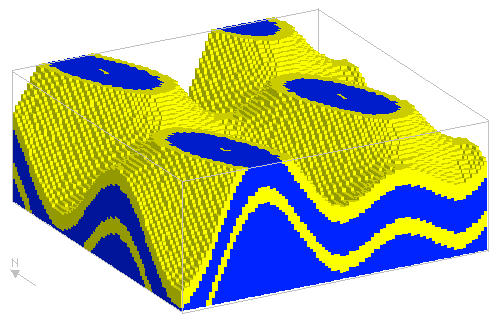
\includegraphics{typeb.jpg}
\caption{Fold interference pattern}\end{figure}

Instead of loading the model into a history object, we are now directly
creating an experiment object:

\begin{Verbatim}[commandchars=\\\{\}]
\PYG{n+nb}{reload}\PYG{p}{(}\PYG{n}{pynoddy}\PYG{o}{.}\PYG{n}{history}\PYG{p}{)}
\PYG{n+nb}{reload}\PYG{p}{(}\PYG{n}{pynoddy}\PYG{o}{.}\PYG{n}{experiment}\PYG{p}{)}

\PYG{k+kn}{from} \PYG{n+nn}{pynoddy.experiment} \PYG{k+kn}{import} \PYG{n}{monte\PYGZus{}carlo}
\PYG{n}{model\PYGZus{}url} \PYG{o}{=} \PYG{l+s}{\PYGZsq{}}\PYG{l+s}{http://tectonique.net/asg/ch3/ch3\PYGZus{}7/his/typeb.his}\PYG{l+s}{\PYGZsq{}}
\PYG{n}{ue} \PYG{o}{=} \PYG{n}{pynoddy}\PYG{o}{.}\PYG{n}{experiment}\PYG{o}{.}\PYG{n}{Experiment}\PYG{p}{(}\PYG{n}{url} \PYG{o}{=} \PYG{n}{model\PYGZus{}url}\PYG{p}{)}
\end{Verbatim}

For simpler visualisation in this notebook, we will analyse the
following steps in a section view of the model.

We consider a section in y-direction through the model:

\begin{Verbatim}[commandchars=\\\{\}]
\PYG{n}{ue}\PYG{o}{.}\PYG{n}{write\PYGZus{}history}\PYG{p}{(}\PYG{l+s}{\PYGZdq{}}\PYG{l+s}{typeb\PYGZus{}tmp3.his}\PYG{l+s}{\PYGZdq{}}\PYG{p}{)}
\end{Verbatim}

\begin{Verbatim}[commandchars=\\\{\}]
\PYG{n}{ue}\PYG{o}{.}\PYG{n}{write\PYGZus{}history}\PYG{p}{(}\PYG{l+s}{\PYGZdq{}}\PYG{l+s}{typeb\PYGZus{}tmp2.his}\PYG{l+s}{\PYGZdq{}}\PYG{p}{)}
\end{Verbatim}

\begin{Verbatim}[commandchars=\\\{\}]
\PYG{n}{ue}\PYG{o}{.}\PYG{n}{change\PYGZus{}cube\PYGZus{}size}\PYG{p}{(}\PYG{l+m+mi}{100}\PYG{p}{)}
\PYG{n}{ue}\PYG{o}{.}\PYG{n}{plot\PYGZus{}section}\PYG{p}{(}\PYG{l+s}{\PYGZsq{}}\PYG{l+s}{y}\PYG{l+s}{\PYGZsq{}}\PYG{p}{)}
\end{Verbatim}

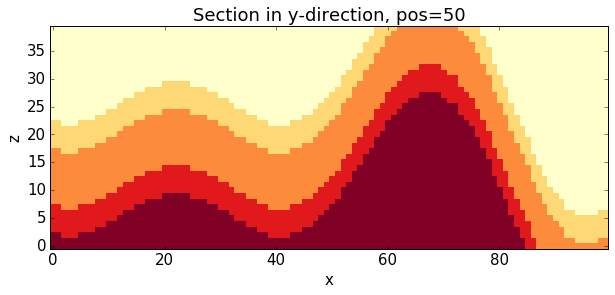
\includegraphics{6-Reproducible-Experiments_10_0.png}

Before we start to draw random realisations of the model, we should
first store the base state of the model for later reference. This is
simply possibel with the freeze() method which stores the current state
of the model as the ``base-state'':

\begin{Verbatim}[commandchars=\\\{\}]
\PYG{n}{ue}\PYG{o}{.}\PYG{n}{freeze}\PYG{p}{(}\PYG{p}{)}
\end{Verbatim}

We now intialise the random generator. We can directly assign a random
seed to simplify reproducibility (note that this is not \emph{essential}, as
it would be for the definition in a script function: the random state is
preserved within the model and could be retrieved at a later stage, as
well!):

\begin{Verbatim}[commandchars=\\\{\}]
\PYG{n}{ue}\PYG{o}{.}\PYG{n}{set\PYGZus{}random\PYGZus{}seed}\PYG{p}{(}\PYG{l+m+mi}{12345}\PYG{p}{)}
\end{Verbatim}

The next step is to define probability distributions to the relevant
event parameters. Let's first look at the different events:

\begin{Verbatim}[commandchars=\\\{\}]
\PYG{n}{ue}\PYG{o}{.}\PYG{n}{info}\PYG{p}{(}\PYG{n}{events\PYGZus{}only} \PYG{o}{=} \PYG{n+nb+bp}{True}\PYG{p}{)}
\end{Verbatim}

\begin{Verbatim}[commandchars=\\\{\}]
This model consists of 3 events:
    (1) \PYGZhy{} STRATIGRAPHY
    (2) \PYGZhy{} FOLD
    (3) \PYGZhy{} FOLD
\end{Verbatim}

\begin{Verbatim}[commandchars=\\\{\}]
\PYG{n}{ev2} \PYG{o}{=} \PYG{n}{ue}\PYG{o}{.}\PYG{n}{events}\PYG{p}{[}\PYG{l+m+mi}{2}\PYG{p}{]}
\end{Verbatim}

\begin{Verbatim}[commandchars=\\\{\}]
\PYG{n}{ev2}\PYG{o}{.}\PYG{n}{properties}
\end{Verbatim}

\begin{Verbatim}[commandchars=\\\{\}]
\PYG{p}{\PYGZob{}}\PYG{l+s}{\PYGZsq{}}\PYG{l+s}{Amplitude}\PYG{l+s}{\PYGZsq{}}\PYG{p}{:} \PYG{l+m+mf}{1250.0}\PYG{p}{,}
 \PYG{l+s}{\PYGZsq{}}\PYG{l+s}{Cylindricity}\PYG{l+s}{\PYGZsq{}}\PYG{p}{:} \PYG{l+m+mf}{0.0}\PYG{p}{,}
 \PYG{l+s}{\PYGZsq{}}\PYG{l+s}{Dip}\PYG{l+s}{\PYGZsq{}}\PYG{p}{:} \PYG{l+m+mf}{90.0}\PYG{p}{,}
 \PYG{l+s}{\PYGZsq{}}\PYG{l+s}{Dip Direction}\PYG{l+s}{\PYGZsq{}}\PYG{p}{:} \PYG{l+m+mf}{90.0}\PYG{p}{,}
 \PYG{l+s}{\PYGZsq{}}\PYG{l+s}{Pitch}\PYG{l+s}{\PYGZsq{}}\PYG{p}{:} \PYG{l+m+mf}{0.0}\PYG{p}{,}
 \PYG{l+s}{\PYGZsq{}}\PYG{l+s}{Single Fold}\PYG{l+s}{\PYGZsq{}}\PYG{p}{:} \PYG{l+s}{\PYGZsq{}}\PYG{l+s}{FALSE}\PYG{l+s}{\PYGZsq{}}\PYG{p}{,}
 \PYG{l+s}{\PYGZsq{}}\PYG{l+s}{Type}\PYG{l+s}{\PYGZsq{}}\PYG{p}{:} \PYG{l+s}{\PYGZsq{}}\PYG{l+s}{Sine}\PYG{l+s}{\PYGZsq{}}\PYG{p}{,}
 \PYG{l+s}{\PYGZsq{}}\PYG{l+s}{Wavelength}\PYG{l+s}{\PYGZsq{}}\PYG{p}{:} \PYG{l+m+mf}{5000.0}\PYG{p}{,}
 \PYG{l+s}{\PYGZsq{}}\PYG{l+s}{X}\PYG{l+s}{\PYGZsq{}}\PYG{p}{:} \PYG{l+m+mf}{1000.0}\PYG{p}{,}
 \PYG{l+s}{\PYGZsq{}}\PYG{l+s}{Y}\PYG{l+s}{\PYGZsq{}}\PYG{p}{:} \PYG{l+m+mf}{0.0}\PYG{p}{,}
 \PYG{l+s}{\PYGZsq{}}\PYG{l+s}{Z}\PYG{l+s}{\PYGZsq{}}\PYG{p}{:} \PYG{l+m+mf}{0.0}\PYG{p}{\PYGZcb{}}
\end{Verbatim}

Next, we define the probability distributions for the uncertain input
parameters:

\begin{Verbatim}[commandchars=\\\{\}]
\PYG{n}{param\PYGZus{}stats} \PYG{o}{=} \PYG{p}{[}\PYG{p}{\PYGZob{}}\PYG{l+s}{\PYGZsq{}}\PYG{l+s}{event}\PYG{l+s}{\PYGZsq{}} \PYG{p}{:} \PYG{l+m+mi}{2}\PYG{p}{,}
              \PYG{l+s}{\PYGZsq{}}\PYG{l+s}{parameter}\PYG{l+s}{\PYGZsq{}}\PYG{p}{:} \PYG{l+s}{\PYGZsq{}}\PYG{l+s}{Amplitude}\PYG{l+s}{\PYGZsq{}}\PYG{p}{,}
              \PYG{l+s}{\PYGZsq{}}\PYG{l+s}{stdev}\PYG{l+s}{\PYGZsq{}}\PYG{p}{:} \PYG{l+m+mf}{100.0}\PYG{p}{,}
              \PYG{l+s}{\PYGZsq{}}\PYG{l+s}{type}\PYG{l+s}{\PYGZsq{}}\PYG{p}{:} \PYG{l+s}{\PYGZsq{}}\PYG{l+s}{normal}\PYG{l+s}{\PYGZsq{}}\PYG{p}{\PYGZcb{}}\PYG{p}{,}
              \PYG{p}{\PYGZob{}}\PYG{l+s}{\PYGZsq{}}\PYG{l+s}{event}\PYG{l+s}{\PYGZsq{}} \PYG{p}{:} \PYG{l+m+mi}{2}\PYG{p}{,}
              \PYG{l+s}{\PYGZsq{}}\PYG{l+s}{parameter}\PYG{l+s}{\PYGZsq{}}\PYG{p}{:} \PYG{l+s}{\PYGZsq{}}\PYG{l+s}{Wavelength}\PYG{l+s}{\PYGZsq{}}\PYG{p}{,}
              \PYG{l+s}{\PYGZsq{}}\PYG{l+s}{stdev}\PYG{l+s}{\PYGZsq{}}\PYG{p}{:} \PYG{l+m+mf}{500.0}\PYG{p}{,}
              \PYG{l+s}{\PYGZsq{}}\PYG{l+s}{type}\PYG{l+s}{\PYGZsq{}}\PYG{p}{:} \PYG{l+s}{\PYGZsq{}}\PYG{l+s}{normal}\PYG{l+s}{\PYGZsq{}}\PYG{p}{\PYGZcb{}}\PYG{p}{,}
              \PYG{p}{\PYGZob{}}\PYG{l+s}{\PYGZsq{}}\PYG{l+s}{event}\PYG{l+s}{\PYGZsq{}} \PYG{p}{:} \PYG{l+m+mi}{2}\PYG{p}{,}
              \PYG{l+s}{\PYGZsq{}}\PYG{l+s}{parameter}\PYG{l+s}{\PYGZsq{}}\PYG{p}{:} \PYG{l+s}{\PYGZsq{}}\PYG{l+s}{X}\PYG{l+s}{\PYGZsq{}}\PYG{p}{,}
              \PYG{l+s}{\PYGZsq{}}\PYG{l+s}{stdev}\PYG{l+s}{\PYGZsq{}}\PYG{p}{:} \PYG{l+m+mf}{500.0}\PYG{p}{,}
              \PYG{l+s}{\PYGZsq{}}\PYG{l+s}{type}\PYG{l+s}{\PYGZsq{}}\PYG{p}{:} \PYG{l+s}{\PYGZsq{}}\PYG{l+s}{normal}\PYG{l+s}{\PYGZsq{}}\PYG{p}{\PYGZcb{}}\PYG{p}{]}

\PYG{n}{ue}\PYG{o}{.}\PYG{n}{set\PYGZus{}parameter\PYGZus{}statistics}\PYG{p}{(}\PYG{n}{param\PYGZus{}stats}\PYG{p}{)}
\end{Verbatim}

\begin{Verbatim}[commandchars=\\\{\}]
\PYG{n}{resolution} \PYG{o}{=} \PYG{l+m+mi}{100}
\PYG{n}{ue}\PYG{o}{.}\PYG{n}{change\PYGZus{}cube\PYGZus{}size}\PYG{p}{(}\PYG{n}{resolution}\PYG{p}{)}
\PYG{n}{tmp} \PYG{o}{=} \PYG{n}{ue}\PYG{o}{.}\PYG{n}{get\PYGZus{}section}\PYG{p}{(}\PYG{l+s}{\PYGZsq{}}\PYG{l+s}{y}\PYG{l+s}{\PYGZsq{}}\PYG{p}{)}
\PYG{n}{prob\PYGZus{}4} \PYG{o}{=} \PYG{n}{np}\PYG{o}{.}\PYG{n}{zeros\PYGZus{}like}\PYG{p}{(}\PYG{n}{tmp}\PYG{o}{.}\PYG{n}{block}\PYG{p}{[}\PYG{p}{:}\PYG{p}{,}\PYG{p}{:}\PYG{p}{,}\PYG{p}{:}\PYG{p}{]}\PYG{p}{)}
\PYG{n}{n\PYGZus{}draws} \PYG{o}{=} \PYG{l+m+mi}{100}


\PYG{k}{for} \PYG{n}{i} \PYG{o+ow}{in} \PYG{n+nb}{range}\PYG{p}{(}\PYG{n}{n\PYGZus{}draws}\PYG{p}{)}\PYG{p}{:}
    \PYG{n}{ue}\PYG{o}{.}\PYG{n}{random\PYGZus{}draw}\PYG{p}{(}\PYG{p}{)}
    \PYG{n}{tmp} \PYG{o}{=} \PYG{n}{ue}\PYG{o}{.}\PYG{n}{get\PYGZus{}section}\PYG{p}{(}\PYG{l+s}{\PYGZsq{}}\PYG{l+s}{y}\PYG{l+s}{\PYGZsq{}}\PYG{p}{,} \PYG{n}{resolution} \PYG{o}{=} \PYG{n}{resolution}\PYG{p}{)}
    \PYG{n}{prob\PYGZus{}4} \PYG{o}{+}\PYG{o}{=} \PYG{p}{(}\PYG{n}{tmp}\PYG{o}{.}\PYG{n}{block}\PYG{p}{[}\PYG{p}{:}\PYG{p}{,}\PYG{p}{:}\PYG{p}{,}\PYG{p}{:}\PYG{p}{]} \PYG{o}{==} \PYG{l+m+mi}{4}\PYG{p}{)}

\PYG{c}{\PYGZsh{} Normalise}
\PYG{n}{prob\PYGZus{}4} \PYG{o}{=} \PYG{n}{prob\PYGZus{}4} \PYG{o}{/} \PYG{n+nb}{float}\PYG{p}{(}\PYG{n}{n\PYGZus{}draws}\PYG{p}{)}
\end{Verbatim}

\begin{Verbatim}[commandchars=\\\{\}]
\PYG{n}{fig} \PYG{o}{=} \PYG{n}{plt}\PYG{o}{.}\PYG{n}{figure}\PYG{p}{(}\PYG{n}{figsize} \PYG{o}{=} \PYG{p}{(}\PYG{l+m+mi}{12}\PYG{p}{,}\PYG{l+m+mi}{8}\PYG{p}{)}\PYG{p}{)}
\PYG{n}{ax} \PYG{o}{=} \PYG{n}{fig}\PYG{o}{.}\PYG{n}{add\PYGZus{}subplot}\PYG{p}{(}\PYG{l+m+mi}{111}\PYG{p}{)}
\PYG{n}{ax}\PYG{o}{.}\PYG{n}{imshow}\PYG{p}{(}\PYG{n}{prob\PYGZus{}4}\PYG{o}{.}\PYG{n}{transpose}\PYG{p}{(}\PYG{p}{)}\PYG{p}{[}\PYG{p}{:}\PYG{p}{,}\PYG{l+m+mi}{0}\PYG{p}{,}\PYG{p}{:}\PYG{p}{]}\PYG{p}{,}
           \PYG{n}{origin} \PYG{o}{=} \PYG{l+s}{\PYGZsq{}}\PYG{l+s}{lower left}\PYG{l+s}{\PYGZsq{}}\PYG{p}{,}
           \PYG{n}{interpolation} \PYG{o}{=} \PYG{l+s}{\PYGZsq{}}\PYG{l+s}{none}\PYG{l+s}{\PYGZsq{}}\PYG{p}{)}
\PYG{n}{plt}\PYG{o}{.}\PYG{n}{title}\PYG{p}{(}\PYG{l+s}{\PYGZdq{}}\PYG{l+s}{Estimated probability of unit 4}\PYG{l+s}{\PYGZdq{}}\PYG{p}{)}
\PYG{n}{plt}\PYG{o}{.}\PYG{n}{xlabel}\PYG{p}{(}\PYG{l+s}{\PYGZdq{}}\PYG{l+s}{x (E\PYGZhy{}W)}\PYG{l+s}{\PYGZdq{}}\PYG{p}{)}
\PYG{n}{plt}\PYG{o}{.}\PYG{n}{ylabel}\PYG{p}{(}\PYG{l+s}{\PYGZdq{}}\PYG{l+s}{z}\PYG{l+s}{\PYGZdq{}}\PYG{p}{)}
\end{Verbatim}

\begin{Verbatim}[commandchars=\\\{\}]
\PYGZlt{}matplotlib.text.Text at 0x10ba80250\PYGZgt{}
\end{Verbatim}

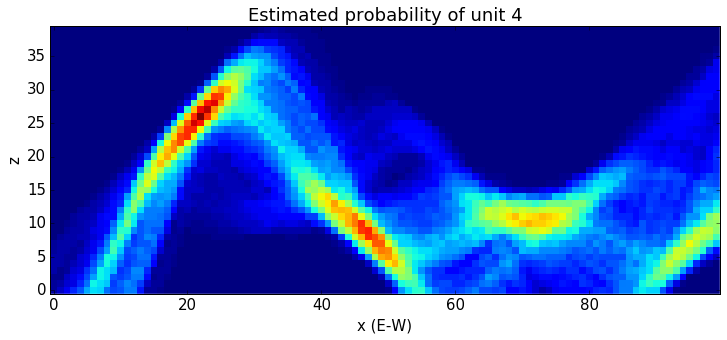
\includegraphics{6-Reproducible-Experiments_22_1.png}

This example shows how the base module for reproducible experiments with
kinematics can be used. For further specification, child classes of
\code{Experiment} can be defined, and we show examples of this type of
extension in the next sections.


\chapter{Gippsland Basin Uncertainty Study}
\label{notebooks/7-Gippsland-Basin-Uncertainty::doc}\label{notebooks/7-Gippsland-Basin-Uncertainty:gippsland-basin-uncertainty-study}
\begin{Verbatim}[commandchars=\\\{\}]
\PYG{k+kn}{from} \PYG{n+nn}{IPython.core.display} \PYG{k+kn}{import} \PYG{n}{HTML}
\PYG{n}{css\PYGZus{}file} \PYG{o}{=} \PYG{l+s}{\PYGZsq{}}\PYG{l+s}{pynoddy.css}\PYG{l+s}{\PYGZsq{}}
\PYG{n}{HTML}\PYG{p}{(}\PYG{n+nb}{open}\PYG{p}{(}\PYG{n}{css\PYGZus{}file}\PYG{p}{,} \PYG{l+s}{\PYGZdq{}}\PYG{l+s}{r}\PYG{l+s}{\PYGZdq{}}\PYG{p}{)}\PYG{o}{.}\PYG{n}{read}\PYG{p}{(}\PYG{p}{)}\PYG{p}{)}
\end{Verbatim}

\begin{Verbatim}[commandchars=\\\{\}]
\PYGZpc{}matplotlib inline
\end{Verbatim}

\begin{Verbatim}[commandchars=\\\{\}]
\PYG{c}{\PYGZsh{}import the ususal libraries + the pynoddy UncertaintyAnalysis class}

\PYG{k+kn}{import} \PYG{n+nn}{sys}\PYG{o}{,} \PYG{n+nn}{os}\PYG{o}{,} \PYG{n+nn}{pynoddy}
\PYG{c}{\PYGZsh{} from pynoddy.experiment.UncertaintyAnalysis import UncertaintyAnalysis}

\PYG{c}{\PYGZsh{} adjust some settings for matplotlib}
\PYG{k+kn}{from} \PYG{n+nn}{matplotlib} \PYG{k+kn}{import} \PYG{n}{rcParams}
\PYG{c}{\PYGZsh{} print rcParams}
\PYG{n}{rcParams}\PYG{p}{[}\PYG{l+s}{\PYGZsq{}}\PYG{l+s}{font.size}\PYG{l+s}{\PYGZsq{}}\PYG{p}{]} \PYG{o}{=} \PYG{l+m+mi}{15}

\PYG{c}{\PYGZsh{} determine path of repository to set paths corretly below}
\PYG{n}{repo\PYGZus{}path} \PYG{o}{=} \PYG{n}{os}\PYG{o}{.}\PYG{n}{path}\PYG{o}{.}\PYG{n}{realpath}\PYG{p}{(}\PYG{l+s}{\PYGZsq{}}\PYG{l+s}{../..}\PYG{l+s}{\PYGZsq{}}\PYG{p}{)}
\PYG{k+kn}{import} \PYG{n+nn}{pynoddy.history}
\PYG{k+kn}{import} \PYG{n+nn}{pynoddy.experiment.uncertainty\PYGZus{}analysis}
\PYG{n}{rcParams}\PYG{o}{.}\PYG{n}{update}\PYG{p}{(}\PYG{p}{\PYGZob{}}\PYG{l+s}{\PYGZsq{}}\PYG{l+s}{font.size}\PYG{l+s}{\PYGZsq{}}\PYG{p}{:} \PYG{l+m+mi}{20}\PYG{p}{\PYGZcb{}}\PYG{p}{)}
\end{Verbatim}


\section{The Gippsland Basin Model}
\label{notebooks/7-Gippsland-Basin-Uncertainty:the-gippsland-basin-model}
In this example we will apply the UncertaintyAnalysis class we have been
playing with in the previous example to a `realistic' (though highly
simplified) geological model of the Gippsland Basin, a petroleum field
south of Victoria, Australia. The model has been included as part of the
PyNoddy directory, and can be found at
\code{pynoddy/examples/GBasin\_Ve1\_V4.his}

\begin{Verbatim}[commandchars=\\\{\}]
\PYG{n+nb}{reload}\PYG{p}{(}\PYG{n}{pynoddy}\PYG{o}{.}\PYG{n}{history}\PYG{p}{)}
\PYG{n+nb}{reload}\PYG{p}{(}\PYG{n}{pynoddy}\PYG{o}{.}\PYG{n}{output}\PYG{p}{)}
\PYG{n+nb}{reload}\PYG{p}{(}\PYG{n}{pynoddy}\PYG{o}{.}\PYG{n}{experiment}\PYG{o}{.}\PYG{n}{uncertainty\PYGZus{}analysis}\PYG{p}{)}
\PYG{n+nb}{reload}\PYG{p}{(}\PYG{n}{pynoddy}\PYG{p}{)}

\PYG{c}{\PYGZsh{} the model itself is now part of the repository, in the examples directory:}
\PYG{n}{history\PYGZus{}file} \PYG{o}{=} \PYG{n}{os}\PYG{o}{.}\PYG{n}{path}\PYG{o}{.}\PYG{n}{join}\PYG{p}{(}\PYG{n}{repo\PYGZus{}path}\PYG{p}{,} \PYG{l+s}{\PYGZdq{}}\PYG{l+s}{examples/GBasin\PYGZus{}Ve1\PYGZus{}V4.his}\PYG{l+s}{\PYGZdq{}}\PYG{p}{)}
\end{Verbatim}

While we could hard-code parameter variations here, it is much easier to
store our statistical information in a csv file, so we load that
instead. This file accompanies the \code{GBasin\_Ve1\_V4} model in the
pynoddy directory.

\begin{Verbatim}[commandchars=\\\{\}]
\PYG{n}{params} \PYG{o}{=} \PYG{n}{os}\PYG{o}{.}\PYG{n}{path}\PYG{o}{.}\PYG{n}{join}\PYG{p}{(}\PYG{n}{repo\PYGZus{}path}\PYG{p}{,}\PYG{l+s}{\PYGZdq{}}\PYG{l+s}{examples/gipps\PYGZus{}params.csv}\PYG{l+s}{\PYGZdq{}}\PYG{p}{)}
\end{Verbatim}


\section{Generate randomised model realisations}
\label{notebooks/7-Gippsland-Basin-Uncertainty:generate-randomised-model-realisations}
Now we have all the information required to perform a Monte-Carlo based
uncertainty analysis. In this example we will generate 100 model
realisations and use them to estimate the information entropy of each
voxel in the model, and hence visualise uncertainty. It is worth noting
that in reality we would need to produce several thousand model
realisations in order to adequately sample the model space, however for
convinience we only generate a small number of models here.

\begin{Verbatim}[commandchars=\\\{\}]
\PYG{c}{\PYGZsh{} \PYGZpc{}\PYGZpc{}timeit   \PYGZsh{} Uncomment to test execution time}
\PYG{n}{ua} \PYG{o}{=} \PYG{n}{pynoddy}\PYG{o}{.}\PYG{n}{experiment}\PYG{o}{.}\PYG{n}{uncertainty\PYGZus{}analysis}\PYG{o}{.}\PYG{n}{UncertaintyAnalysis}\PYG{p}{(}\PYG{n}{history\PYGZus{}file}\PYG{p}{,} \PYG{n}{params}\PYG{p}{)}
\PYG{n}{ua}\PYG{o}{.}\PYG{n}{estimate\PYGZus{}uncertainty}\PYG{p}{(}\PYG{l+m+mi}{100}\PYG{p}{,}\PYG{n}{verbose}\PYG{o}{=}\PYG{n+nb+bp}{False}\PYG{p}{)}
\end{Verbatim}

A few utility functions for visualising uncertainty have been included
in the UncertaintyAnalysis class, and can be used to gain an
understanding of the most uncertain parts of the Gippsland Basin. The
probabability voxets for each lithology can also be accessed using
\code{ua.p\_block{[}lithology\_id{]}}, and the information entropy voxset
accessed using \code{ua.e\_block}.

Note that the Gippsland Basin model has been computed with a vertical
exaggeration of 3, in order to highlight vertical structure.

\begin{Verbatim}[commandchars=\\\{\}]
\PYG{n}{ua}\PYG{o}{.}\PYG{n}{plot\PYGZus{}section}\PYG{p}{(}\PYG{n}{direction}\PYG{o}{=}\PYG{l+s}{\PYGZsq{}}\PYG{l+s}{x}\PYG{l+s}{\PYGZsq{}}\PYG{p}{,}\PYG{n}{data}\PYG{o}{=}\PYG{n}{ua}\PYG{o}{.}\PYG{n}{block}\PYG{p}{)}
\PYG{n}{ua}\PYG{o}{.}\PYG{n}{plot\PYGZus{}entropy}\PYG{p}{(}\PYG{n}{direction}\PYG{o}{=}\PYG{l+s}{\PYGZsq{}}\PYG{l+s}{x}\PYG{l+s}{\PYGZsq{}}\PYG{p}{)}
\end{Verbatim}

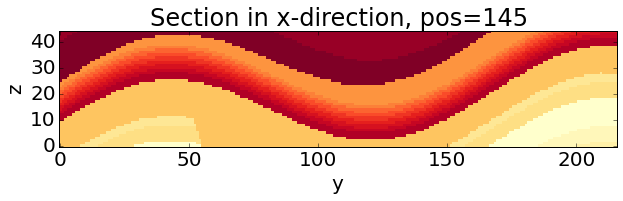
\includegraphics{7-Gippsland-Basin-Uncertainty_11_0.png}

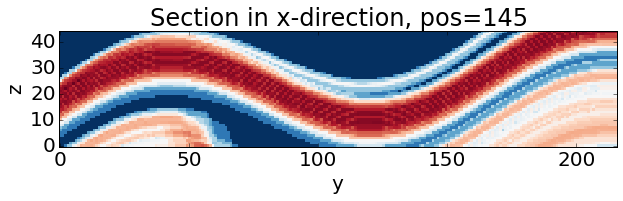
\includegraphics{7-Gippsland-Basin-Uncertainty_11_1.png}

It is immediately apparent (and not particularly surprising) that
uncertainty in the Gippsland Basin model is concentrated around the thin
(but economically interesting) formations comprising the La Trobe and
Strzelecki Groups. The faults in the model also contribute to this
uncertainty, though not by a huge amount.

<<<<<<< HEAD
\chapter{Stochastic events}
\label{notebooks/4-Stochastic-Events::doc}\label{notebooks/4-Stochastic-Events:stochastic-events}
The parameters defining the geological events are, by their very nature,
highly uncertain. In addition to these uncertainties, the kinematic
approach by itself is only a limiting approximation. The picture that we
obtain from the kinematic forword model is therefore a very
overconfident repsresentation of reality - an aspect that (hopefully)
everyone using Noddy is aware of...

In order to respect the vast nature of these uncertainties, we introduce
here an adapted version of the standard geological events defined in
Noddy: the definition of a stochastic event:

A stochastic event is geological event in the Noddy history that has an
uncertainty associated to it in such a way that, recomputing the
geolgoical history will result in a different result each time (note:
the definition is borrowed from the notion of stochastic events in
probabilistic programming, see for example pymc).


\section{Definition of stochastic events}
\label{notebooks/4-Stochastic-Events:definition-of-stochastic-events}
We start, as before, with a pre-defined geological noddy history for
simplicity:


\chapter{pynoddy package}
\label{pynoddy:pynoddy-package}\label{pynoddy::doc}

\section{Submodules}
\label{pynoddy:submodules}

\section{pynoddy.history module}
\label{pynoddy:pynoddy-history-module}\label{pynoddy:module-pynoddy.history}\index{pynoddy.history (module)}
Noddy history file wrapper
Created on 24/03/2014
=======

\section{Exporting results to VTK for visualisation}
\label{notebooks/7-Gippsland-Basin-Uncertainty:exporting-results-to-vtk-for-visualisation}
It is also possible (and useful!) to export the uncertainty information
to .vtk format for 3D analysis in software such as ParaView. This can be
done as follows:

\begin{Verbatim}[commandchars=\\\{\}]
\PYG{n}{ua}\PYG{o}{.}\PYG{n}{extent\PYGZus{}x} \PYG{o}{=} \PYG{l+m+mi}{29000}
\PYG{n}{ua}\PYG{o}{.}\PYG{n}{extent\PYGZus{}y} \PYG{o}{=} \PYG{l+m+mi}{21600}
\PYG{n}{ua}\PYG{o}{.}\PYG{n}{extent\PYGZus{}z} \PYG{o}{=} \PYG{l+m+mi}{4500}

\PYG{n}{output\PYGZus{}path} \PYG{o}{=} \PYG{n}{os}\PYG{o}{.}\PYG{n}{path}\PYG{o}{.}\PYG{n}{join}\PYG{p}{(}\PYG{n}{repo\PYGZus{}path}\PYG{p}{,}\PYG{l+s}{\PYGZdq{}}\PYG{l+s}{sandbox/GBasin\PYGZus{}Uncertainty}\PYG{l+s}{\PYGZdq{}}\PYG{p}{)}
\PYG{n}{ua}\PYG{o}{.}\PYG{n}{export\PYGZus{}to\PYGZus{}vtk}\PYG{p}{(}\PYG{n}{vtk\PYGZus{}filename}\PYG{o}{=}\PYG{n}{output\PYGZus{}path}\PYG{p}{,}\PYG{n}{data}\PYG{o}{=}\PYG{n}{ua}\PYG{o}{.}\PYG{n}{e\PYGZus{}block}\PYG{p}{)}
\end{Verbatim}

The resulting vtr file can (in the sandbox directory) can now be loaded
and properly analysed in a 3D visualisation package such as ParaView.
\begin{figure}[htbp]
\centering
\capstart

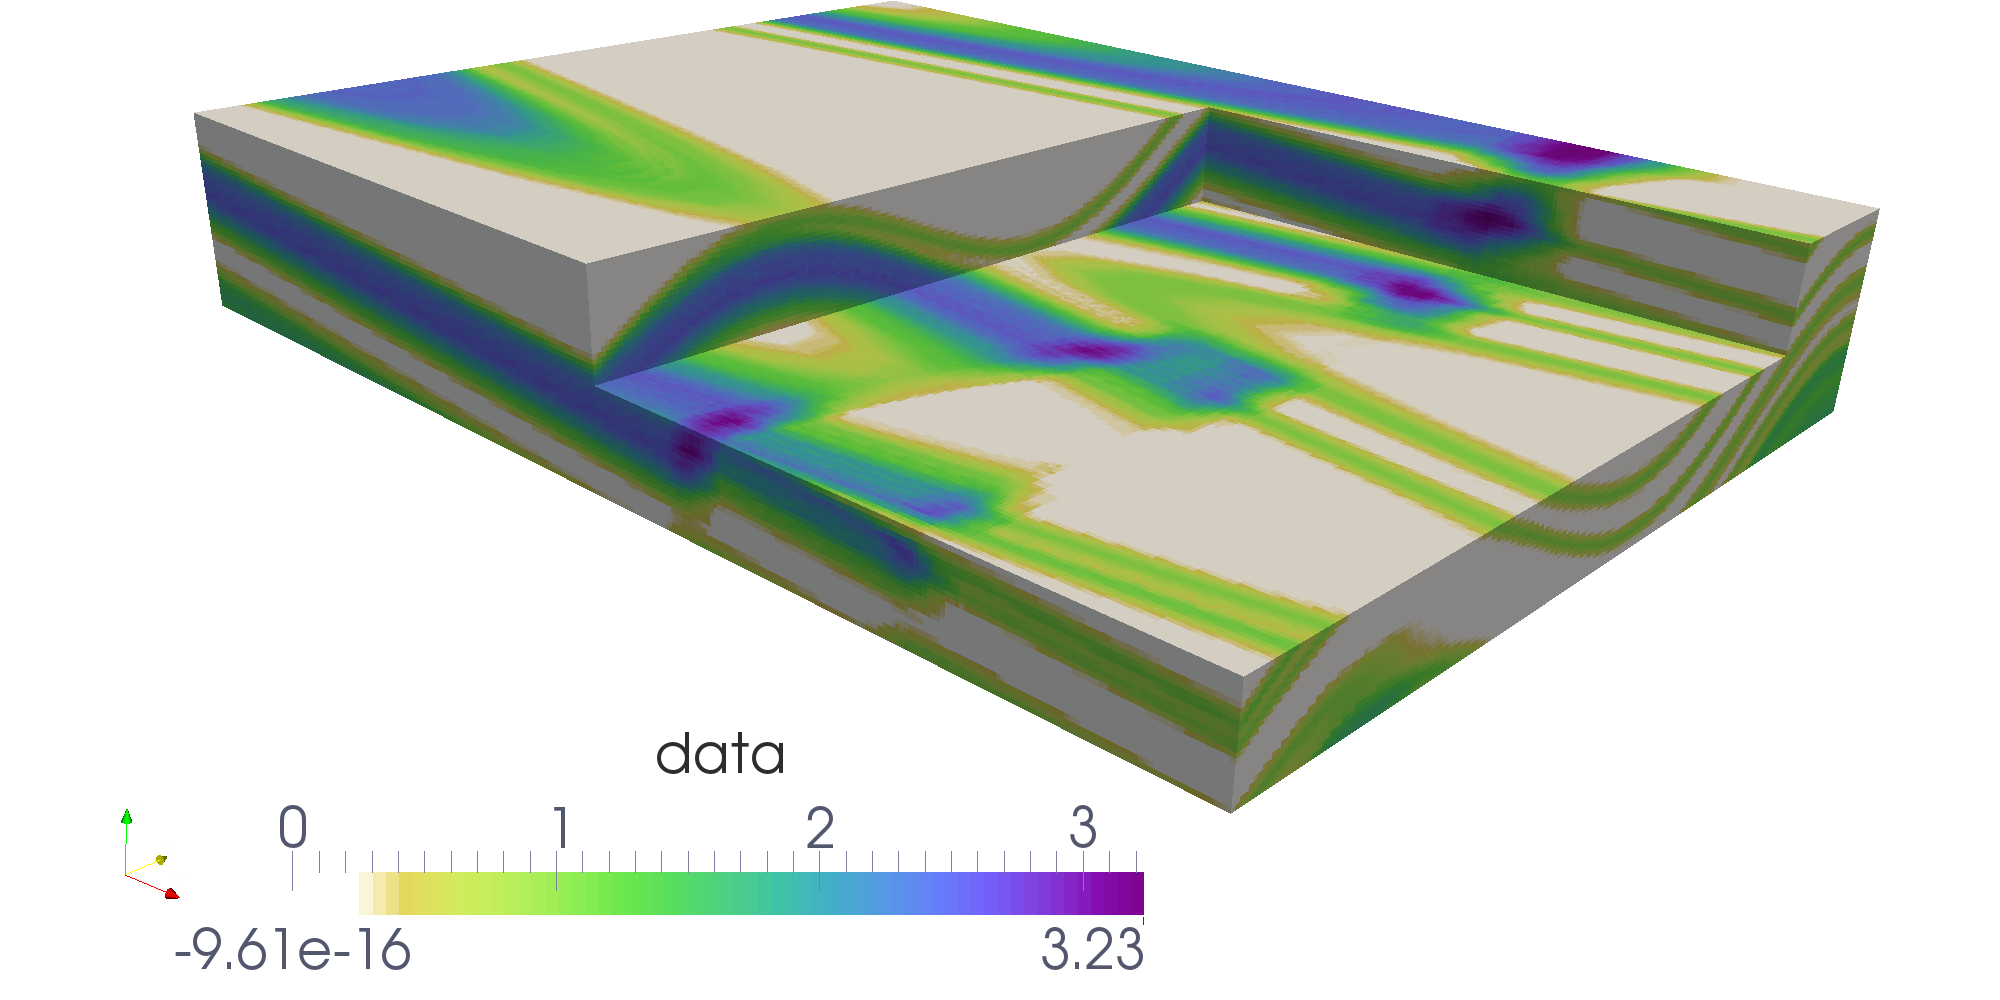
\includegraphics{3D-render.png}
\caption{3-D visualisation of cell information entropy}\end{figure}


\chapter{Sensitivity Analysis}
\label{notebooks/8-Sensitivity-Analysis:sensitivity-analysis}\label{notebooks/8-Sensitivity-Analysis::doc}
Test here: (local) sensitivity analysis of kinematic parameters with
respect to a defined objective function. Aim: test how sensitivity the
resulting model is to uncertainties in kinematic parameters to:
\begin{enumerate}
\item {} 
Evaluate which the most important parameters are, and to

\item {} 
Determine which parameters could, in principle, be inverted with
suitable information.

\end{enumerate}
>>>>>>> refs/remotes/flohorovicic/master


<<<<<<< HEAD
\begin{fulllineitems}
\phantomsection\label{pynoddy:pynoddy.history.NoddyHistory}\pysiglinewithargsret{\strong{class }\code{pynoddy.history.}\bfcode{NoddyHistory}}{\emph{history}}{}
Class container for Noddy history files
\index{change\_cube\_size() (pynoddy.history.NoddyHistory method)}

\begin{fulllineitems}
\phantomsection\label{pynoddy:pynoddy.history.NoddyHistory.change_cube_size}\pysiglinewithargsret{\bfcode{change\_cube\_size}}{\emph{cube\_size}}{}
Change the model cube size (isotropic)
\begin{description}
\item[{\textbf{Arguments}:}] \leavevmode\begin{itemize}
\item {} 
\emph{cube\_size} = float : new model cube size
=======
\section{Theory: local sensitivity analysis}
\label{notebooks/8-Sensitivity-Analysis:theory-local-sensitivity-analysis}
Basic considerations:
\begin{itemize}
\item {} 
parameter vector \(\vec{p}\)

\item {} 
residual vector \(\vec{r}\)

\item {} 
calculated values at observation points \(\vec{z}\)

\item {} 
Jacobian matrix
\(J_{ij} = \frac{\partial \vec{z}}{\partial \vec{p}}\)

\end{itemize}

Numerical estimation of Jacobian matrix with central difference scheme
(see Finsterle):
\begin{gather}
\begin{split}J_{ij} = \frac{\partial z_i}{\partial p_j} \approx \frac{z_i(\vec{p}; p_j + \delta p_j) - z_i(\vec{p};p_j - \delta p_j)}{2 \delta p_j}\end{split}\notag
\end{gather}
where \(\delta p_j\) is a small perturbation of parameter \(j\),
often as a fraction of the value.


\section{Defining the responses}
\label{notebooks/8-Sensitivity-Analysis:defining-the-responses}
A meaningful sensitivity analysis obviously depends on the definition of
a suitable response vector \(\vec{z}\). Ideally, these responses are
related to actual observations. In our case, we first want to determine
how sensitive a kinematic structural geological model is with respect to
uncertainties in the kinematic parameters. We therefore need
calculatable measures that describe variations of the model.

As a first-order assumption, we will use a notation of a stratigraphic
distance for discrete subsections of the model, for example in single
voxets for the calculated model. We define distance \(d\) of a
subset \(\omega\) as the (discrete) difference between the
(discrete) stratigraphic value of an ideal model, \(\hat{s}\), to
the value of a model realisation \(s_i\):
\begin{gather}
\begin{split}d(\omega) = \hat{s} - s_i\end{split}\notag
\end{gather}
In the first example, we will consider only one response: the overall
sum of stratigraphic distances for a model realisation \(r\) of all
subsets (= voxets, in the practical sense), scaled by the number of
subsets (for a subsequent comparison of model discretisations):
\begin{gather}
\begin{split}D_r = \frac{1}{n} \sum_{i=1}^n d(\omega_i)\end{split}\notag
\end{gather}
Note: mistake before: not considering distances at single nodes but only
the sum - this lead to ``zero-difference'' for simple translation! Now:
consider more realistic objective function, squared distance:
\begin{gather}
\begin{split}r = \sqrt{\sum_i (z_{i calc} - z_{i ref})^2}\end{split}\notag
\end{gather}
\begin{Verbatim}[commandchars=\\\{\}]
\PYG{k+kn}{from} \PYG{n+nn}{IPython.core.display} \PYG{k+kn}{import} \PYG{n}{HTML}
\PYG{n}{css\PYGZus{}file} \PYG{o}{=} \PYG{l+s}{\PYGZsq{}}\PYG{l+s}{pynoddy.css}\PYG{l+s}{\PYGZsq{}}
\PYG{n}{HTML}\PYG{p}{(}\PYG{n+nb}{open}\PYG{p}{(}\PYG{n}{css\PYGZus{}file}\PYG{p}{,} \PYG{l+s}{\PYGZdq{}}\PYG{l+s}{r}\PYG{l+s}{\PYGZdq{}}\PYG{p}{)}\PYG{o}{.}\PYG{n}{read}\PYG{p}{(}\PYG{p}{)}\PYG{p}{)}
\end{Verbatim}

\begin{Verbatim}[commandchars=\\\{\}]
\PYGZpc{}matplotlib inline
\end{Verbatim}


\section{Setting up the base model}
\label{notebooks/8-Sensitivity-Analysis:setting-up-the-base-model}
For a first test: use simple two-fault model from paper

\begin{Verbatim}[commandchars=\\\{\}]
\PYG{k+kn}{import} \PYG{n+nn}{sys}\PYG{o}{,} \PYG{n+nn}{os}
\PYG{k+kn}{import} \PYG{n+nn}{matplotlib.pyplot} \PYG{k+kn}{as} \PYG{n+nn}{plt}
\PYG{k+kn}{import} \PYG{n+nn}{numpy} \PYG{k+kn}{as} \PYG{n+nn}{np}
\PYG{c}{\PYGZsh{} adjust some settings for matplotlib}
\PYG{k+kn}{from} \PYG{n+nn}{matplotlib} \PYG{k+kn}{import} \PYG{n}{rcParams}
\PYG{c}{\PYGZsh{} print rcParams}
\PYG{n}{rcParams}\PYG{p}{[}\PYG{l+s}{\PYGZsq{}}\PYG{l+s}{font.size}\PYG{l+s}{\PYGZsq{}}\PYG{p}{]} \PYG{o}{=} \PYG{l+m+mi}{15}
\PYG{c}{\PYGZsh{} determine path of repository to set paths corretly below}
\PYG{n}{repo\PYGZus{}path} \PYG{o}{=} \PYG{n}{os}\PYG{o}{.}\PYG{n}{path}\PYG{o}{.}\PYG{n}{realpath}\PYG{p}{(}\PYG{l+s}{\PYGZsq{}}\PYG{l+s}{../..}\PYG{l+s}{\PYGZsq{}}\PYG{p}{)}
\PYG{k+kn}{import} \PYG{n+nn}{pynoddy.history}
\PYG{k+kn}{import} \PYG{n+nn}{pynoddy.events}
\PYG{k+kn}{import} \PYG{n+nn}{pynoddy.output}
\end{Verbatim}

\begin{Verbatim}[commandchars=\\\{\}]
\PYG{n+nb}{reload}\PYG{p}{(}\PYG{n}{pynoddy}\PYG{o}{.}\PYG{n}{history}\PYG{p}{)}
\PYG{n+nb}{reload}\PYG{p}{(}\PYG{n}{pynoddy}\PYG{o}{.}\PYG{n}{events}\PYG{p}{)}
\PYG{n}{nm} \PYG{o}{=} \PYG{n}{pynoddy}\PYG{o}{.}\PYG{n}{history}\PYG{o}{.}\PYG{n}{NoddyHistory}\PYG{p}{(}\PYG{p}{)}
\PYG{c}{\PYGZsh{} add stratigraphy}
\PYG{n}{strati\PYGZus{}options} \PYG{o}{=} \PYG{p}{\PYGZob{}}\PYG{l+s}{\PYGZsq{}}\PYG{l+s}{num\PYGZus{}layers}\PYG{l+s}{\PYGZsq{}} \PYG{p}{:} \PYG{l+m+mi}{8}\PYG{p}{,}
                  \PYG{l+s}{\PYGZsq{}}\PYG{l+s}{layer\PYGZus{}names}\PYG{l+s}{\PYGZsq{}} \PYG{p}{:} \PYG{p}{[}\PYG{l+s}{\PYGZsq{}}\PYG{l+s}{layer 1}\PYG{l+s}{\PYGZsq{}}\PYG{p}{,} \PYG{l+s}{\PYGZsq{}}\PYG{l+s}{layer 2}\PYG{l+s}{\PYGZsq{}}\PYG{p}{,} \PYG{l+s}{\PYGZsq{}}\PYG{l+s}{layer 3}\PYG{l+s}{\PYGZsq{}}\PYG{p}{,} \PYG{l+s}{\PYGZsq{}}\PYG{l+s}{layer 4}\PYG{l+s}{\PYGZsq{}}\PYG{p}{,} \PYG{l+s}{\PYGZsq{}}\PYG{l+s}{layer 5}\PYG{l+s}{\PYGZsq{}}\PYG{p}{,} \PYG{l+s}{\PYGZsq{}}\PYG{l+s}{layer 6}\PYG{l+s}{\PYGZsq{}}\PYG{p}{,} \PYG{l+s}{\PYGZsq{}}\PYG{l+s}{layer 7}\PYG{l+s}{\PYGZsq{}}\PYG{p}{,} \PYG{l+s}{\PYGZsq{}}\PYG{l+s}{layer 8}\PYG{l+s}{\PYGZsq{}}\PYG{p}{]}\PYG{p}{,}
                  \PYG{l+s}{\PYGZsq{}}\PYG{l+s}{layer\PYGZus{}thickness}\PYG{l+s}{\PYGZsq{}} \PYG{p}{:} \PYG{p}{[}\PYG{l+m+mi}{1500}\PYG{p}{,} \PYG{l+m+mi}{500}\PYG{p}{,} \PYG{l+m+mi}{500}\PYG{p}{,} \PYG{l+m+mi}{500}\PYG{p}{,} \PYG{l+m+mi}{500}\PYG{p}{,} \PYG{l+m+mi}{500}\PYG{p}{,} \PYG{l+m+mi}{500}\PYG{p}{,} \PYG{l+m+mi}{500}\PYG{p}{]}\PYG{p}{\PYGZcb{}}
\PYG{n}{nm}\PYG{o}{.}\PYG{n}{add\PYGZus{}event}\PYG{p}{(}\PYG{l+s}{\PYGZsq{}}\PYG{l+s}{stratigraphy}\PYG{l+s}{\PYGZsq{}}\PYG{p}{,} \PYG{n}{strati\PYGZus{}options} \PYG{p}{)}

\PYG{c}{\PYGZsh{} The following options define the fault geometry:}
\PYG{n}{fault\PYGZus{}options} \PYG{o}{=} \PYG{p}{\PYGZob{}}\PYG{l+s}{\PYGZsq{}}\PYG{l+s}{name}\PYG{l+s}{\PYGZsq{}} \PYG{p}{:} \PYG{l+s}{\PYGZsq{}}\PYG{l+s}{Fault\PYGZus{}W}\PYG{l+s}{\PYGZsq{}}\PYG{p}{,}
                 \PYG{l+s}{\PYGZsq{}}\PYG{l+s}{pos}\PYG{l+s}{\PYGZsq{}} \PYG{p}{:} \PYG{p}{(}\PYG{l+m+mi}{4000}\PYG{p}{,} \PYG{l+m+mi}{3500}\PYG{p}{,} \PYG{l+m+mi}{5000}\PYG{p}{)}\PYG{p}{,}
                 \PYG{l+s}{\PYGZsq{}}\PYG{l+s}{dip\PYGZus{}dir}\PYG{l+s}{\PYGZsq{}} \PYG{p}{:} \PYG{l+m+mi}{90}\PYG{p}{,}
                 \PYG{l+s}{\PYGZsq{}}\PYG{l+s}{dip}\PYG{l+s}{\PYGZsq{}} \PYG{p}{:} \PYG{l+m+mi}{60}\PYG{p}{,}
                 \PYG{l+s}{\PYGZsq{}}\PYG{l+s}{slip}\PYG{l+s}{\PYGZsq{}} \PYG{p}{:} \PYG{l+m+mi}{1000}\PYG{p}{\PYGZcb{}}

\PYG{n}{nm}\PYG{o}{.}\PYG{n}{add\PYGZus{}event}\PYG{p}{(}\PYG{l+s}{\PYGZsq{}}\PYG{l+s}{fault}\PYG{l+s}{\PYGZsq{}}\PYG{p}{,} \PYG{n}{fault\PYGZus{}options}\PYG{p}{)}
\PYG{c}{\PYGZsh{} The following options define the fault geometry:}
\PYG{n}{fault\PYGZus{}options} \PYG{o}{=} \PYG{p}{\PYGZob{}}\PYG{l+s}{\PYGZsq{}}\PYG{l+s}{name}\PYG{l+s}{\PYGZsq{}} \PYG{p}{:} \PYG{l+s}{\PYGZsq{}}\PYG{l+s}{Fault\PYGZus{}E}\PYG{l+s}{\PYGZsq{}}\PYG{p}{,}
                 \PYG{l+s}{\PYGZsq{}}\PYG{l+s}{pos}\PYG{l+s}{\PYGZsq{}} \PYG{p}{:} \PYG{p}{(}\PYG{l+m+mi}{6000}\PYG{p}{,} \PYG{l+m+mi}{3500}\PYG{p}{,} \PYG{l+m+mi}{5000}\PYG{p}{)}\PYG{p}{,}
                 \PYG{l+s}{\PYGZsq{}}\PYG{l+s}{dip\PYGZus{}dir}\PYG{l+s}{\PYGZsq{}} \PYG{p}{:} \PYG{l+m+mi}{270}\PYG{p}{,}
                 \PYG{l+s}{\PYGZsq{}}\PYG{l+s}{dip}\PYG{l+s}{\PYGZsq{}} \PYG{p}{:} \PYG{l+m+mi}{60}\PYG{p}{,}
                 \PYG{l+s}{\PYGZsq{}}\PYG{l+s}{slip}\PYG{l+s}{\PYGZsq{}} \PYG{p}{:} \PYG{l+m+mi}{1000}\PYG{p}{\PYGZcb{}}

\PYG{n}{nm}\PYG{o}{.}\PYG{n}{add\PYGZus{}event}\PYG{p}{(}\PYG{l+s}{\PYGZsq{}}\PYG{l+s}{fault}\PYG{l+s}{\PYGZsq{}}\PYG{p}{,} \PYG{n}{fault\PYGZus{}options}\PYG{p}{)}
\PYG{n}{history} \PYG{o}{=} \PYG{l+s}{\PYGZdq{}}\PYG{l+s}{two\PYGZus{}faults\PYGZus{}sensi.his}\PYG{l+s}{\PYGZdq{}}
\PYG{n}{nm}\PYG{o}{.}\PYG{n}{write\PYGZus{}history}\PYG{p}{(}\PYG{n}{history}\PYG{p}{)}
\end{Verbatim}

\begin{Verbatim}[commandchars=\\\{\}]
\PYG{n}{output\PYGZus{}name} \PYG{o}{=} \PYG{l+s}{\PYGZdq{}}\PYG{l+s}{two\PYGZus{}faults\PYGZus{}sensi\PYGZus{}out}\PYG{l+s}{\PYGZdq{}}
\PYG{c}{\PYGZsh{} Compute the model}
\PYG{n}{pynoddy}\PYG{o}{.}\PYG{n}{compute\PYGZus{}model}\PYG{p}{(}\PYG{n}{history}\PYG{p}{,} \PYG{n}{output\PYGZus{}name}\PYG{p}{)}
\end{Verbatim}

\begin{Verbatim}[commandchars=\\\{\}]
\PYG{l+s}{\PYGZsq{}}\PYG{l+s}{\PYGZsq{}}
\end{Verbatim}

\begin{Verbatim}[commandchars=\\\{\}]
\PYG{c}{\PYGZsh{} Plot output}
\PYG{n}{nout} \PYG{o}{=} \PYG{n}{pynoddy}\PYG{o}{.}\PYG{n}{output}\PYG{o}{.}\PYG{n}{NoddyOutput}\PYG{p}{(}\PYG{n}{output\PYGZus{}name}\PYG{p}{)}
\PYG{n}{nout}\PYG{o}{.}\PYG{n}{plot\PYGZus{}section}\PYG{p}{(}\PYG{l+s}{\PYGZsq{}}\PYG{l+s}{y}\PYG{l+s}{\PYGZsq{}}\PYG{p}{,} \PYG{n}{layer\PYGZus{}labels} \PYG{o}{=} \PYG{n}{strati\PYGZus{}options}\PYG{p}{[}\PYG{l+s}{\PYGZsq{}}\PYG{l+s}{layer\PYGZus{}names}\PYG{l+s}{\PYGZsq{}}\PYG{p}{]}\PYG{p}{[}\PYG{p}{:}\PYG{p}{:}\PYG{o}{\PYGZhy{}}\PYG{l+m+mi}{1}\PYG{p}{]}\PYG{p}{,}
                  \PYG{n}{colorbar} \PYG{o}{=} \PYG{n+nb+bp}{True}\PYG{p}{,} \PYG{n}{title}\PYG{o}{=}\PYG{l+s}{\PYGZdq{}}\PYG{l+s}{\PYGZdq{}}\PYG{p}{,}
                  \PYG{n}{savefig} \PYG{o}{=} \PYG{n+nb+bp}{False}\PYG{p}{)}
\end{Verbatim}

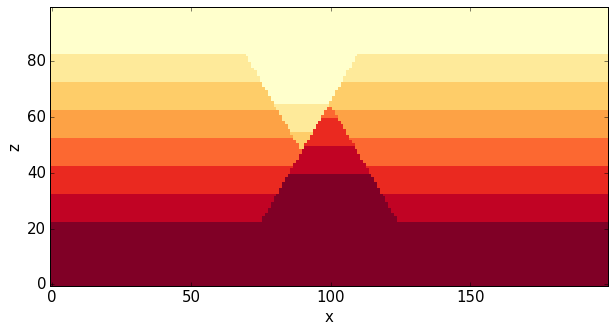
\includegraphics{8-Sensitivity-Analysis_7_0.png}


\section{Define parameter uncertainties}
\label{notebooks/8-Sensitivity-Analysis:define-parameter-uncertainties}
We will start with a sensitivity analysis for the parameters of the
fault events.

\begin{Verbatim}[commandchars=\\\{\}]
\PYG{n}{H1} \PYG{o}{=} \PYG{n}{pynoddy}\PYG{o}{.}\PYG{n}{history}\PYG{o}{.}\PYG{n}{NoddyHistory}\PYG{p}{(}\PYG{n}{history}\PYG{p}{)}
\PYG{c}{\PYGZsh{} get the original dip of the fault}
\PYG{n}{dip\PYGZus{}ori} \PYG{o}{=} \PYG{n}{H1}\PYG{o}{.}\PYG{n}{events}\PYG{p}{[}\PYG{l+m+mi}{3}\PYG{p}{]}\PYG{o}{.}\PYG{n}{properties}\PYG{p}{[}\PYG{l+s}{\PYGZsq{}}\PYG{l+s}{Dip}\PYG{l+s}{\PYGZsq{}}\PYG{p}{]}
\PYG{c}{\PYGZsh{} dip\PYGZus{}ori1 = H1.events[2].properties[\PYGZsq{}Dip\PYGZsq{}]}
\PYG{c}{\PYGZsh{} add 10 degrees to dip}
\PYG{n}{add\PYGZus{}dip} \PYG{o}{=} \PYG{o}{\PYGZhy{}}\PYG{l+m+mi}{20}
\PYG{n}{dip\PYGZus{}new} \PYG{o}{=} \PYG{n}{dip\PYGZus{}ori} \PYG{o}{+} \PYG{n}{add\PYGZus{}dip}
\PYG{c}{\PYGZsh{} dip\PYGZus{}new1 = dip\PYGZus{}ori1 + add\PYGZus{}dip}

\PYG{c}{\PYGZsh{} and assign back to properties dictionary:}
\PYG{n}{H1}\PYG{o}{.}\PYG{n}{events}\PYG{p}{[}\PYG{l+m+mi}{3}\PYG{p}{]}\PYG{o}{.}\PYG{n}{properties}\PYG{p}{[}\PYG{l+s}{\PYGZsq{}}\PYG{l+s}{Dip}\PYG{l+s}{\PYGZsq{}}\PYG{p}{]} \PYG{o}{=} \PYG{n}{dip\PYGZus{}new}
\end{Verbatim}

\begin{Verbatim}[commandchars=\\\{\}]
\PYG{n+nb}{reload}\PYG{p}{(}\PYG{n}{pynoddy}\PYG{o}{.}\PYG{n}{output}\PYG{p}{)}
\PYG{n}{new\PYGZus{}history} \PYG{o}{=} \PYG{l+s}{\PYGZdq{}}\PYG{l+s}{sensi\PYGZus{}test\PYGZus{}dip\PYGZus{}changed.his}\PYG{l+s}{\PYGZdq{}}
\PYG{n}{new\PYGZus{}output} \PYG{o}{=} \PYG{l+s}{\PYGZdq{}}\PYG{l+s}{sensi\PYGZus{}test\PYGZus{}dip\PYGZus{}changed\PYGZus{}out}\PYG{l+s}{\PYGZdq{}}
\PYG{n}{H1}\PYG{o}{.}\PYG{n}{write\PYGZus{}history}\PYG{p}{(}\PYG{n}{new\PYGZus{}history}\PYG{p}{)}
\PYG{n}{pynoddy}\PYG{o}{.}\PYG{n}{compute\PYGZus{}model}\PYG{p}{(}\PYG{n}{new\PYGZus{}history}\PYG{p}{,} \PYG{n}{new\PYGZus{}output}\PYG{p}{)}
\PYG{c}{\PYGZsh{} load output from both models}
\PYG{n}{NO1} \PYG{o}{=} \PYG{n}{pynoddy}\PYG{o}{.}\PYG{n}{output}\PYG{o}{.}\PYG{n}{NoddyOutput}\PYG{p}{(}\PYG{n}{output\PYGZus{}name}\PYG{p}{)}
\PYG{n}{NO2} \PYG{o}{=} \PYG{n}{pynoddy}\PYG{o}{.}\PYG{n}{output}\PYG{o}{.}\PYG{n}{NoddyOutput}\PYG{p}{(}\PYG{n}{new\PYGZus{}output}\PYG{p}{)}

\PYG{c}{\PYGZsh{} create basic figure layout}
\PYG{n}{fig} \PYG{o}{=} \PYG{n}{plt}\PYG{o}{.}\PYG{n}{figure}\PYG{p}{(}\PYG{n}{figsize} \PYG{o}{=} \PYG{p}{(}\PYG{l+m+mi}{15}\PYG{p}{,}\PYG{l+m+mi}{5}\PYG{p}{)}\PYG{p}{)}
\PYG{n}{ax1} \PYG{o}{=} \PYG{n}{fig}\PYG{o}{.}\PYG{n}{add\PYGZus{}subplot}\PYG{p}{(}\PYG{l+m+mi}{121}\PYG{p}{)}
\PYG{n}{ax2} \PYG{o}{=} \PYG{n}{fig}\PYG{o}{.}\PYG{n}{add\PYGZus{}subplot}\PYG{p}{(}\PYG{l+m+mi}{122}\PYG{p}{)}
\PYG{n}{NO1}\PYG{o}{.}\PYG{n}{plot\PYGZus{}section}\PYG{p}{(}\PYG{l+s}{\PYGZsq{}}\PYG{l+s}{y}\PYG{l+s}{\PYGZsq{}}\PYG{p}{,} \PYG{n}{position}\PYG{o}{=}\PYG{l+m+mi}{0}\PYG{p}{,} \PYG{n}{ax} \PYG{o}{=} \PYG{n}{ax1}\PYG{p}{,} \PYG{n}{colorbar}\PYG{o}{=}\PYG{n+nb+bp}{False}\PYG{p}{,} \PYG{n}{title}\PYG{o}{=}\PYG{l+s}{\PYGZdq{}}\PYG{l+s}{Dip = }\PYG{l+s+si}{\PYGZpc{}.0f}\PYG{l+s}{\PYGZdq{}} \PYG{o}{\PYGZpc{}} \PYG{n}{dip\PYGZus{}ori}\PYG{p}{)}
\PYG{n}{NO2}\PYG{o}{.}\PYG{n}{plot\PYGZus{}section}\PYG{p}{(}\PYG{l+s}{\PYGZsq{}}\PYG{l+s}{y}\PYG{l+s}{\PYGZsq{}}\PYG{p}{,} \PYG{n}{position}\PYG{o}{=}\PYG{l+m+mi}{0}\PYG{p}{,} \PYG{n}{ax} \PYG{o}{=} \PYG{n}{ax2}\PYG{p}{,} \PYG{n}{colorbar}\PYG{o}{=}\PYG{n+nb+bp}{False}\PYG{p}{,} \PYG{n}{title}\PYG{o}{=}\PYG{l+s}{\PYGZdq{}}\PYG{l+s}{Dip = }\PYG{l+s+si}{\PYGZpc{}.0f}\PYG{l+s}{\PYGZdq{}} \PYG{o}{\PYGZpc{}} \PYG{n}{dip\PYGZus{}new}\PYG{p}{)}

\PYG{n}{plt}\PYG{o}{.}\PYG{n}{show}\PYG{p}{(}\PYG{p}{)}
\end{Verbatim}

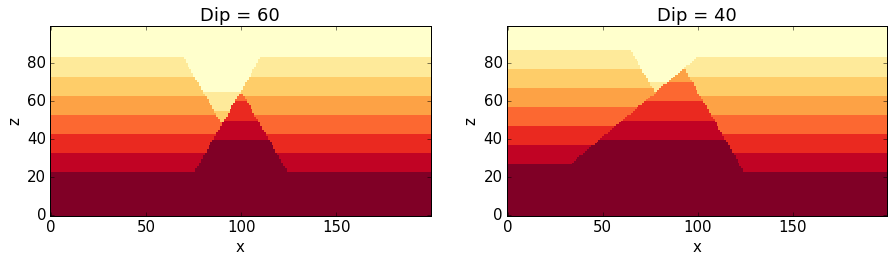
\includegraphics{8-Sensitivity-Analysis_10_0.png}
>>>>>>> refs/remotes/flohorovicic/master


\section{Calculate total stratigraphic distance}
\label{notebooks/8-Sensitivity-Analysis:calculate-total-stratigraphic-distance}
\begin{Verbatim}[commandchars=\\\{\}]
\PYG{c}{\PYGZsh{} def determine\PYGZus{}strati\PYGZus{}diff(NO1, NO2):}
\PYG{c}{\PYGZsh{}     \PYGZdq{}\PYGZdq{}\PYGZdq{}calculate total stratigraphic distance between two models\PYGZdq{}\PYGZdq{}\PYGZdq{}}
\PYG{c}{\PYGZsh{}     return np.sum(NO1.block \PYGZhy{} NO2.block) / float(len(NO1.block))}

\PYG{k}{def} \PYG{n+nf}{determine\PYGZus{}strati\PYGZus{}diff}\PYG{p}{(}\PYG{n}{NO1}\PYG{p}{,} \PYG{n}{NO2}\PYG{p}{)}\PYG{p}{:}
    \PYG{l+s+sd}{\PYGZdq{}\PYGZdq{}\PYGZdq{}calculate total stratigraphic distance between two models\PYGZdq{}\PYGZdq{}\PYGZdq{}}
    \PYG{k}{return} \PYG{n}{np}\PYG{o}{.}\PYG{n}{sqrt}\PYG{p}{(}\PYG{n}{np}\PYG{o}{.}\PYG{n}{sum}\PYG{p}{(}\PYG{p}{(}\PYG{n}{NO1}\PYG{o}{.}\PYG{n}{block} \PYG{o}{\PYGZhy{}} \PYG{n}{NO2}\PYG{o}{.}\PYG{n}{block}\PYG{p}{)}\PYG{o}{*}\PYG{o}{*}\PYG{l+m+mi}{2}\PYG{p}{)}\PYG{p}{)} \PYG{o}{/} \PYG{n+nb}{float}\PYG{p}{(}\PYG{n+nb}{len}\PYG{p}{(}\PYG{n}{NO1}\PYG{o}{.}\PYG{n}{block}\PYG{p}{)}\PYG{p}{)}

<<<<<<< HEAD
\index{determine\_events() (pynoddy.history.NoddyHistory method)}

\begin{fulllineitems}
\phantomsection\label{pynoddy:pynoddy.history.NoddyHistory.determine_events}\pysiglinewithargsret{\bfcode{determine\_events}}{}{}
Determine events and save line numbers

\begin{notice}{note}{Note:}
Parsing of the history file is based on a fixed Noddy output order. 
If this is, for some reason (e.g. in a changed version of Noddy) not the case, then
this parsing might fail!
\end{notice}
=======


\PYG{n}{diff} \PYG{o}{=} \PYG{n}{determine\PYGZus{}strati\PYGZus{}diff}\PYG{p}{(}\PYG{n}{NO1}\PYG{p}{,} \PYG{n}{NO2}\PYG{p}{)}
\PYG{k}{print}\PYG{p}{(}\PYG{n}{diff}\PYG{p}{)}
\end{Verbatim}

\begin{Verbatim}[commandchars=\\\{\}]
\PYG{l+m+mf}{5.56205897128}
\end{Verbatim}


\section{Function to modify parameters}
\label{notebooks/8-Sensitivity-Analysis:function-to-modify-parameters}
Multiple event parameters can be changed directly with the function
\code{change\_event\_params}, which takes a dictionarly of events and
parameters with according changes relative to the defined parameters.
Here a brief example:

\begin{Verbatim}[commandchars=\\\{\}]
\PYG{c}{\PYGZsh{} set parameter changes in dictionary}

\PYG{n}{changes\PYGZus{}fault\PYGZus{}1} \PYG{o}{=} \PYG{p}{\PYGZob{}}\PYG{l+s}{\PYGZsq{}}\PYG{l+s}{Dip}\PYG{l+s}{\PYGZsq{}} \PYG{p}{:} \PYG{o}{\PYGZhy{}}\PYG{l+m+mi}{20}\PYG{p}{\PYGZcb{}}
\PYG{n}{changes\PYGZus{}fault\PYGZus{}2} \PYG{o}{=} \PYG{p}{\PYGZob{}}\PYG{l+s}{\PYGZsq{}}\PYG{l+s}{Dip}\PYG{l+s}{\PYGZsq{}} \PYG{p}{:} \PYG{o}{\PYGZhy{}}\PYG{l+m+mi}{20}\PYG{p}{\PYGZcb{}}
\PYG{n}{param\PYGZus{}changes} \PYG{o}{=} \PYG{p}{\PYGZob{}}\PYG{l+m+mi}{2} \PYG{p}{:} \PYG{n}{changes\PYGZus{}fault\PYGZus{}1}\PYG{p}{,}
                 \PYG{l+m+mi}{3} \PYG{p}{:} \PYG{n}{changes\PYGZus{}fault\PYGZus{}2}\PYG{p}{\PYGZcb{}}
\end{Verbatim}

\begin{Verbatim}[commandchars=\\\{\}]
\PYG{n+nb}{reload}\PYG{p}{(}\PYG{n}{pynoddy}\PYG{o}{.}\PYG{n}{history}\PYG{p}{)}
\PYG{n}{H2} \PYG{o}{=} \PYG{n}{pynoddy}\PYG{o}{.}\PYG{n}{history}\PYG{o}{.}\PYG{n}{NoddyHistory}\PYG{p}{(}\PYG{n}{history}\PYG{p}{)}
\PYG{n}{H2}\PYG{o}{.}\PYG{n}{change\PYGZus{}event\PYGZus{}params}\PYG{p}{(}\PYG{n}{param\PYGZus{}changes}\PYG{p}{)}
\end{Verbatim}

\begin{Verbatim}[commandchars=\\\{\}]
\PYG{n}{new\PYGZus{}history} \PYG{o}{=} \PYG{l+s}{\PYGZdq{}}\PYG{l+s}{param\PYGZus{}dict\PYGZus{}changes.his}\PYG{l+s}{\PYGZdq{}}
\PYG{n}{new\PYGZus{}output} \PYG{o}{=} \PYG{l+s}{\PYGZdq{}}\PYG{l+s}{param\PYGZus{}dict\PYGZus{}changes\PYGZus{}out}\PYG{l+s}{\PYGZdq{}}
\PYG{n}{H2}\PYG{o}{.}\PYG{n}{write\PYGZus{}history}\PYG{p}{(}\PYG{n}{new\PYGZus{}history}\PYG{p}{)}
\PYG{n}{pynoddy}\PYG{o}{.}\PYG{n}{compute\PYGZus{}model}\PYG{p}{(}\PYG{n}{new\PYGZus{}history}\PYG{p}{,} \PYG{n}{new\PYGZus{}output}\PYG{p}{)}
\PYG{c}{\PYGZsh{} load output from both models}
\PYG{n}{NO1} \PYG{o}{=} \PYG{n}{pynoddy}\PYG{o}{.}\PYG{n}{output}\PYG{o}{.}\PYG{n}{NoddyOutput}\PYG{p}{(}\PYG{n}{output\PYGZus{}name}\PYG{p}{)}
\PYG{n}{NO2} \PYG{o}{=} \PYG{n}{pynoddy}\PYG{o}{.}\PYG{n}{output}\PYG{o}{.}\PYG{n}{NoddyOutput}\PYG{p}{(}\PYG{n}{new\PYGZus{}output}\PYG{p}{)}

\PYG{c}{\PYGZsh{} create basic figure layout}
\PYG{n}{fig} \PYG{o}{=} \PYG{n}{plt}\PYG{o}{.}\PYG{n}{figure}\PYG{p}{(}\PYG{n}{figsize} \PYG{o}{=} \PYG{p}{(}\PYG{l+m+mi}{15}\PYG{p}{,}\PYG{l+m+mi}{5}\PYG{p}{)}\PYG{p}{)}
\PYG{n}{ax1} \PYG{o}{=} \PYG{n}{fig}\PYG{o}{.}\PYG{n}{add\PYGZus{}subplot}\PYG{p}{(}\PYG{l+m+mi}{121}\PYG{p}{)}
\PYG{n}{ax2} \PYG{o}{=} \PYG{n}{fig}\PYG{o}{.}\PYG{n}{add\PYGZus{}subplot}\PYG{p}{(}\PYG{l+m+mi}{122}\PYG{p}{)}
\PYG{n}{NO1}\PYG{o}{.}\PYG{n}{plot\PYGZus{}section}\PYG{p}{(}\PYG{l+s}{\PYGZsq{}}\PYG{l+s}{y}\PYG{l+s}{\PYGZsq{}}\PYG{p}{,} \PYG{n}{position}\PYG{o}{=}\PYG{l+m+mi}{0}\PYG{p}{,} \PYG{n}{ax} \PYG{o}{=} \PYG{n}{ax1}\PYG{p}{,} \PYG{n}{colorbar}\PYG{o}{=}\PYG{n+nb+bp}{False}\PYG{p}{,} \PYG{n}{title}\PYG{o}{=}\PYG{l+s}{\PYGZdq{}}\PYG{l+s}{Original Model}\PYG{l+s}{\PYGZdq{}}\PYG{p}{)}
\PYG{n}{NO2}\PYG{o}{.}\PYG{n}{plot\PYGZus{}section}\PYG{p}{(}\PYG{l+s}{\PYGZsq{}}\PYG{l+s}{y}\PYG{l+s}{\PYGZsq{}}\PYG{p}{,} \PYG{n}{position}\PYG{o}{=}\PYG{l+m+mi}{0}\PYG{p}{,} \PYG{n}{ax} \PYG{o}{=} \PYG{n}{ax2}\PYG{p}{,} \PYG{n}{colorbar}\PYG{o}{=}\PYG{n+nb+bp}{False}\PYG{p}{,} \PYG{n}{title}\PYG{o}{=}\PYG{l+s}{\PYGZdq{}}\PYG{l+s}{Changed Model}\PYG{l+s}{\PYGZdq{}}\PYG{p}{)}

\PYG{n}{plt}\PYG{o}{.}\PYG{n}{show}\PYG{p}{(}\PYG{p}{)}
\end{Verbatim}

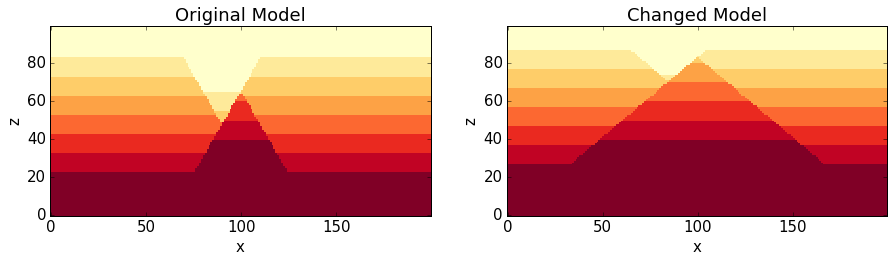
\includegraphics{8-Sensitivity-Analysis_16_0.png}


\section{Full sensitivity analysis}
\label{notebooks/8-Sensitivity-Analysis:full-sensitivity-analysis}
Perform now a full sensitivity analysis for all defined parameters and
analyse the output matrix. For a better overview, we first create a
function to perform the sensitivity analysis:

\begin{Verbatim}[commandchars=\\\{\}]
\PYG{k+kn}{import} \PYG{n+nn}{copy}
\PYG{n}{new\PYGZus{}history} \PYG{o}{=} \PYG{l+s}{\PYGZdq{}}\PYG{l+s}{sensi\PYGZus{}tmp.his}\PYG{l+s}{\PYGZdq{}}
\PYG{n}{new\PYGZus{}output} \PYG{o}{=} \PYG{l+s}{\PYGZdq{}}\PYG{l+s}{sensi\PYGZus{}out}\PYG{l+s}{\PYGZdq{}}
\PYG{k}{def} \PYG{n+nf}{noddy\PYGZus{}sensitivity}\PYG{p}{(}\PYG{n}{history\PYGZus{}filename}\PYG{p}{,} \PYG{n}{param\PYGZus{}change\PYGZus{}vals}\PYG{p}{)}\PYG{p}{:}
    \PYG{l+s+sd}{\PYGZdq{}\PYGZdq{}\PYGZdq{}Perform noddy sensitivity analysis for a model\PYGZdq{}\PYGZdq{}\PYGZdq{}}
    \PYG{n}{param\PYGZus{}list} \PYG{o}{=} \PYG{p}{[}\PYG{p}{]} \PYG{c}{\PYGZsh{} list to store parameters for later analysis}
    \PYG{n}{distances} \PYG{o}{=} \PYG{p}{[}\PYG{p}{]} \PYG{c}{\PYGZsh{} list to store calcualted distances}
    \PYG{c}{\PYGZsh{} Step 1:}
    \PYG{c}{\PYGZsh{} create new parameter list to change model}
    \PYG{k}{for} \PYG{n}{event\PYGZus{}id}\PYG{p}{,} \PYG{n}{event\PYGZus{}dict} \PYG{o+ow}{in} \PYG{n}{param\PYGZus{}change\PYGZus{}vals}\PYG{o}{.}\PYG{n}{items}\PYG{p}{(}\PYG{p}{)}\PYG{p}{:} \PYG{c}{\PYGZsh{} iterate over events}
        \PYG{k}{for} \PYG{n}{key}\PYG{p}{,} \PYG{n}{val} \PYG{o+ow}{in} \PYG{n}{event\PYGZus{}dict}\PYG{o}{.}\PYG{n}{items}\PYG{p}{(}\PYG{p}{)}\PYG{p}{:} \PYG{c}{\PYGZsh{} iterate over all properties separately}
            \PYG{n}{changes\PYGZus{}list} \PYG{o}{=} \PYG{n+nb}{dict}\PYG{p}{(}\PYG{p}{)}
            \PYG{n}{changes\PYGZus{}list}\PYG{p}{[}\PYG{n}{event\PYGZus{}id}\PYG{p}{]} \PYG{o}{=} \PYG{n+nb}{dict}\PYG{p}{(}\PYG{p}{)}
            \PYG{n}{param\PYGZus{}list}\PYG{o}{.}\PYG{n}{append}\PYG{p}{(}\PYG{l+s}{\PYGZdq{}}\PYG{l+s}{event\PYGZus{}}\PYG{l+s+si}{\PYGZpc{}d}\PYG{l+s}{\PYGZus{}property\PYGZus{}}\PYG{l+s+si}{\PYGZpc{}s}\PYG{l+s}{\PYGZdq{}} \PYG{o}{\PYGZpc{}} \PYG{p}{(}\PYG{n}{event\PYGZus{}id}\PYG{p}{,} \PYG{n}{key}\PYG{p}{)}\PYG{p}{)}
            \PYG{k}{for} \PYG{n}{i} \PYG{o+ow}{in} \PYG{n+nb}{range}\PYG{p}{(}\PYG{l+m+mi}{2}\PYG{p}{)}\PYG{p}{:}
                \PYG{c}{\PYGZsh{} calculate positive and negative values}
                \PYG{n}{his} \PYG{o}{=} \PYG{n}{pynoddy}\PYG{o}{.}\PYG{n}{history}\PYG{o}{.}\PYG{n}{NoddyHistory}\PYG{p}{(}\PYG{n}{history\PYGZus{}filename}\PYG{p}{)}
                \PYG{k}{if} \PYG{n}{i} \PYG{o}{==} \PYG{l+m+mi}{0}\PYG{p}{:}
                    \PYG{n}{changes\PYGZus{}list}\PYG{p}{[}\PYG{n}{event\PYGZus{}id}\PYG{p}{]}\PYG{p}{[}\PYG{n}{key}\PYG{p}{]} \PYG{o}{=} \PYG{n}{val}
                    \PYG{c}{\PYGZsh{} set changes}
                    \PYG{n}{his}\PYG{o}{.}\PYG{n}{change\PYGZus{}event\PYGZus{}params}\PYG{p}{(}\PYG{n}{changes\PYGZus{}list}\PYG{p}{)}
                    \PYG{c}{\PYGZsh{} save and calculate model}
                    \PYG{n}{his}\PYG{o}{.}\PYG{n}{write\PYGZus{}history}\PYG{p}{(}\PYG{n}{new\PYGZus{}history}\PYG{p}{)}
                    \PYG{n}{pynoddy}\PYG{o}{.}\PYG{n}{compute\PYGZus{}model}\PYG{p}{(}\PYG{n}{new\PYGZus{}history}\PYG{p}{,} \PYG{n}{new\PYGZus{}output}\PYG{p}{)}
                    \PYG{c}{\PYGZsh{} open output and calculate distance}
                    \PYG{n}{NO\PYGZus{}tmp} \PYG{o}{=} \PYG{n}{pynoddy}\PYG{o}{.}\PYG{n}{output}\PYG{o}{.}\PYG{n}{NoddyOutput}\PYG{p}{(}\PYG{n}{new\PYGZus{}output}\PYG{p}{)}
                    \PYG{n}{dist\PYGZus{}pos} \PYG{o}{=} \PYG{n}{determine\PYGZus{}strati\PYGZus{}diff}\PYG{p}{(}\PYG{n}{NO1}\PYG{p}{,} \PYG{n}{NO\PYGZus{}tmp}\PYG{p}{)}
                    \PYG{n}{NO\PYGZus{}tmp}\PYG{o}{.}\PYG{n}{plot\PYGZus{}section}\PYG{p}{(}\PYG{l+s}{\PYGZsq{}}\PYG{l+s}{y}\PYG{l+s}{\PYGZsq{}}\PYG{p}{,} \PYG{n}{position} \PYG{o}{=} \PYG{l+m+mi}{0}\PYG{p}{,} \PYG{n}{colorbar} \PYG{o}{=} \PYG{n+nb+bp}{False}\PYG{p}{,}
                                        \PYG{n}{title} \PYG{o}{=} \PYG{l+s}{\PYGZdq{}}\PYG{l+s}{Dist: }\PYG{l+s+si}{\PYGZpc{}.2f}\PYG{l+s}{\PYGZdq{}} \PYG{o}{\PYGZpc{}} \PYG{n}{dist\PYGZus{}pos}\PYG{p}{,}
                                        \PYG{n}{savefig} \PYG{o}{=} \PYG{n+nb+bp}{True}\PYG{p}{,}
                                        \PYG{n}{fig\PYGZus{}filename} \PYG{o}{=} \PYG{l+s}{\PYGZdq{}}\PYG{l+s}{event\PYGZus{}}\PYG{l+s+si}{\PYGZpc{}d}\PYG{l+s}{\PYGZus{}property\PYGZus{}}\PYG{l+s+si}{\PYGZpc{}s}\PYG{l+s}{\PYGZus{}val\PYGZus{}}\PYG{l+s+si}{\PYGZpc{}d}\PYG{l+s}{.png}\PYG{l+s}{\PYGZdq{}} \PYGZbs{}
                                        \PYG{o}{\PYGZpc{}} \PYG{p}{(}\PYG{n}{event\PYGZus{}id}\PYG{p}{,} \PYG{n}{key}\PYG{p}{,}\PYG{n}{val}\PYG{p}{)}\PYG{p}{)}
                \PYG{k}{if} \PYG{n}{i} \PYG{o}{==} \PYG{l+m+mi}{1}\PYG{p}{:}
                    \PYG{n}{changes\PYGZus{}list}\PYG{p}{[}\PYG{n}{event\PYGZus{}id}\PYG{p}{]}\PYG{p}{[}\PYG{n}{key}\PYG{p}{]} \PYG{o}{=} \PYG{o}{\PYGZhy{}}\PYG{n}{val}
                    \PYG{n}{his}\PYG{o}{.}\PYG{n}{change\PYGZus{}event\PYGZus{}params}\PYG{p}{(}\PYG{n}{changes\PYGZus{}list}\PYG{p}{)}
                    \PYG{c}{\PYGZsh{} save and calculate model}
                    \PYG{n}{his}\PYG{o}{.}\PYG{n}{write\PYGZus{}history}\PYG{p}{(}\PYG{n}{new\PYGZus{}history}\PYG{p}{)}
                    \PYG{n}{pynoddy}\PYG{o}{.}\PYG{n}{compute\PYGZus{}model}\PYG{p}{(}\PYG{n}{new\PYGZus{}history}\PYG{p}{,} \PYG{n}{new\PYGZus{}output}\PYG{p}{)}
                    \PYG{c}{\PYGZsh{} open output and calculate distance}
                    \PYG{n}{NO\PYGZus{}tmp} \PYG{o}{=} \PYG{n}{pynoddy}\PYG{o}{.}\PYG{n}{output}\PYG{o}{.}\PYG{n}{NoddyOutput}\PYG{p}{(}\PYG{n}{new\PYGZus{}output}\PYG{p}{)}
                    \PYG{n}{dist\PYGZus{}neg} \PYG{o}{=} \PYG{n}{determine\PYGZus{}strati\PYGZus{}diff}\PYG{p}{(}\PYG{n}{NO1}\PYG{p}{,} \PYG{n}{NO\PYGZus{}tmp}\PYG{p}{)}
                    \PYG{n}{NO\PYGZus{}tmp}\PYG{o}{.}\PYG{n}{plot\PYGZus{}section}\PYG{p}{(}\PYG{l+s}{\PYGZsq{}}\PYG{l+s}{y}\PYG{l+s}{\PYGZsq{}}\PYG{p}{,} \PYG{n}{position}\PYG{o}{=}\PYG{l+m+mi}{0}\PYG{p}{,} \PYG{n}{colorbar}\PYG{o}{=}\PYG{n+nb+bp}{False}\PYG{p}{,}
                                        \PYG{n}{title}\PYG{o}{=}\PYG{l+s}{\PYGZdq{}}\PYG{l+s}{Dist: }\PYG{l+s+si}{\PYGZpc{}.2f}\PYG{l+s}{\PYGZdq{}} \PYG{o}{\PYGZpc{}} \PYG{n}{dist\PYGZus{}neg}\PYG{p}{,}
                                        \PYG{n}{savefig}\PYG{o}{=}\PYG{n+nb+bp}{True}\PYG{p}{,}
                                        \PYG{n}{fig\PYGZus{}filename}\PYG{o}{=}\PYG{l+s}{\PYGZdq{}}\PYG{l+s}{event\PYGZus{}}\PYG{l+s+si}{\PYGZpc{}d}\PYG{l+s}{\PYGZus{}property\PYGZus{}}\PYG{l+s+si}{\PYGZpc{}s}\PYG{l+s}{\PYGZus{}val\PYGZus{}}\PYG{l+s+si}{\PYGZpc{}d}\PYG{l+s}{.png}\PYG{l+s}{\PYGZdq{}} \PYGZbs{}
                                        \PYG{o}{\PYGZpc{}} \PYG{p}{(}\PYG{n}{event\PYGZus{}id}\PYG{p}{,} \PYG{n}{key}\PYG{p}{,}\PYG{n}{val}\PYG{p}{)}\PYG{p}{)}
            \PYG{c}{\PYGZsh{} calculate central difference}
            \PYG{n}{central\PYGZus{}diff} \PYG{o}{=} \PYG{p}{(}\PYG{n}{dist\PYGZus{}pos} \PYG{o}{+} \PYG{n}{dist\PYGZus{}neg}\PYG{p}{)} \PYG{o}{/} \PYG{p}{(}\PYG{l+m+mf}{2.}\PYG{p}{)}
            \PYG{n}{distances}\PYG{o}{.}\PYG{n}{append}\PYG{p}{(}\PYG{n}{central\PYGZus{}diff}\PYG{p}{)}
    \PYG{k}{return} \PYG{n}{param\PYGZus{}list}\PYG{p}{,} \PYG{n}{distances}
\end{Verbatim}

As a next step, we define the parameter ranges for the local sensitivity
analysis (i.e. the \(\delta p_j\) from the theoretical description
above):

\begin{Verbatim}[commandchars=\\\{\}]
\PYG{n}{changes\PYGZus{}fault\PYGZus{}1} \PYG{o}{=} \PYG{p}{\PYGZob{}}\PYG{l+s}{\PYGZsq{}}\PYG{l+s}{Dip}\PYG{l+s}{\PYGZsq{}} \PYG{p}{:} \PYG{l+m+mf}{1.5}\PYG{p}{,}
                   \PYG{l+s}{\PYGZsq{}}\PYG{l+s}{Dip Direction}\PYG{l+s}{\PYGZsq{}} \PYG{p}{:} \PYG{l+m+mi}{10}\PYG{p}{,}
                   \PYG{l+s}{\PYGZsq{}}\PYG{l+s}{Slip}\PYG{l+s}{\PYGZsq{}}\PYG{p}{:} \PYG{l+m+mf}{100.0}\PYG{p}{,}
                   \PYG{l+s}{\PYGZsq{}}\PYG{l+s}{X}\PYG{l+s}{\PYGZsq{}}\PYG{p}{:} \PYG{l+m+mf}{500.0}\PYG{p}{\PYGZcb{}}
\PYG{n}{changes\PYGZus{}fault\PYGZus{}2} \PYG{o}{=} \PYG{p}{\PYGZob{}}\PYG{l+s}{\PYGZsq{}}\PYG{l+s}{Dip}\PYG{l+s}{\PYGZsq{}} \PYG{p}{:} \PYG{l+m+mf}{1.5}\PYG{p}{,}
                   \PYG{l+s}{\PYGZsq{}}\PYG{l+s}{Dip Direction}\PYG{l+s}{\PYGZsq{}} \PYG{p}{:} \PYG{l+m+mi}{10}\PYG{p}{,}
                   \PYG{l+s}{\PYGZsq{}}\PYG{l+s}{Slip}\PYG{l+s}{\PYGZsq{}}\PYG{p}{:} \PYG{l+m+mf}{100.0}\PYG{p}{,}
                   \PYG{l+s}{\PYGZsq{}}\PYG{l+s}{X}\PYG{l+s}{\PYGZsq{}}\PYG{p}{:} \PYG{l+m+mf}{500.0}\PYG{p}{\PYGZcb{}}
\PYG{n}{param\PYGZus{}changes} \PYG{o}{=} \PYG{p}{\PYGZob{}}\PYG{l+m+mi}{2} \PYG{p}{:} \PYG{n}{changes\PYGZus{}fault\PYGZus{}1}\PYG{p}{,}
                 \PYG{l+m+mi}{3} \PYG{p}{:} \PYG{n}{changes\PYGZus{}fault\PYGZus{}2}\PYG{p}{\PYGZcb{}}
\end{Verbatim}

And now, we perform the local sensitivity analysis:

\begin{Verbatim}[commandchars=\\\{\}]
\PYG{n}{param\PYGZus{}list\PYGZus{}1}\PYG{p}{,} \PYG{n}{distances} \PYG{o}{=} \PYG{n}{noddy\PYGZus{}sensitivity}\PYG{p}{(}\PYG{n}{history}\PYG{p}{,} \PYG{n}{param\PYGZus{}changes}\PYG{p}{)}
\end{Verbatim}

The function passes back a list of the changed parameters and the
calculated distances according to this change. Let's have a look at the
results:
>>>>>>> refs/remotes/flohorovicic/master

\begin{Verbatim}[commandchars=\\\{\}]
\PYG{k}{for} \PYG{n}{p}\PYG{p}{,}\PYG{n}{d} \PYG{o+ow}{in} \PYG{n+nb}{zip}\PYG{p}{(}\PYG{n}{param\PYGZus{}list\PYGZus{}1}\PYG{p}{,} \PYG{n}{distances}\PYG{p}{)}\PYG{p}{:}
    \PYG{k}{print} \PYG{l+s}{\PYGZdq{}}\PYG{l+s+si}{\PYGZpc{}s}\PYG{l+s}{ }\PYG{l+s+se}{\PYGZbs{}t}\PYG{l+s+se}{\PYGZbs{}t}\PYG{l+s}{ }\PYG{l+s+si}{\PYGZpc{}f}\PYG{l+s}{\PYGZdq{}} \PYG{o}{\PYGZpc{}} \PYG{p}{(}\PYG{n}{p}\PYG{p}{,} \PYG{n}{d}\PYG{p}{)}
\end{Verbatim}

<<<<<<< HEAD
\index{load\_history() (pynoddy.history.NoddyHistory method)}

\begin{fulllineitems}
\phantomsection\label{pynoddy:pynoddy.history.NoddyHistory.load_history}\pysiglinewithargsret{\bfcode{load\_history}}{\emph{history}}{}
Load Noddy history
\begin{description}
\item[{\textbf{Arguments}:}] \leavevmode\begin{itemize}
\item {} 
\emph{history} = string : Name of Noddy history file

\end{itemize}

\end{description}
=======
\begin{Verbatim}[commandchars=\\\{\}]
event\PYGZus{}2\PYGZus{}property\PYGZus{}X           2.716228
event\PYGZus{}2\PYGZus{}property\PYGZus{}Dip                 1.410039
event\PYGZus{}2\PYGZus{}property\PYGZus{}Dip Direction               2.133553
event\PYGZus{}2\PYGZus{}property\PYGZus{}Slip                1.824993
event\PYGZus{}3\PYGZus{}property\PYGZus{}X           3.323528
event\PYGZus{}3\PYGZus{}property\PYGZus{}Dip                 1.644589
event\PYGZus{}3\PYGZus{}property\PYGZus{}Dip Direction               2.606573
event\PYGZus{}3\PYGZus{}property\PYGZus{}Slip                1.930455
\end{Verbatim}

Results of this local sensitivity analysis suggest that the model is
most sensitive to the X-position of the fault, when we evaluate
distances as simple stratigraphic id differences. Here just a bar plot
for better visualisation (feel free to add proper labels):

\begin{Verbatim}[commandchars=\\\{\}]
\PYG{n}{d} \PYG{o}{=} \PYG{n}{np}\PYG{o}{.}\PYG{n}{array}\PYG{p}{(}\PYG{p}{[}\PYG{n}{distances}\PYG{p}{]}\PYG{p}{)}
\PYG{n}{fig} \PYG{o}{=} \PYG{n}{plt}\PYG{o}{.}\PYG{n}{figure}\PYG{p}{(}\PYG{n}{figsize}\PYG{o}{=}\PYG{p}{(}\PYG{l+m+mi}{5}\PYG{p}{,}\PYG{l+m+mi}{3}\PYG{p}{)}\PYG{p}{)}
\PYG{n}{ax} \PYG{o}{=} \PYG{n}{fig}\PYG{o}{.}\PYG{n}{add\PYGZus{}subplot}\PYG{p}{(}\PYG{l+m+mi}{111}\PYG{p}{)}
\PYG{n}{ax}\PYG{o}{.}\PYG{n}{bar}\PYG{p}{(}\PYG{n}{np}\PYG{o}{.}\PYG{n}{arange}\PYG{p}{(}\PYG{l+m+mf}{0.6}\PYG{p}{,}\PYG{n+nb}{len}\PYG{p}{(}\PYG{n}{distances}\PYG{p}{)}\PYG{p}{,}\PYG{l+m+mf}{1.}\PYG{p}{)}\PYG{p}{,} \PYG{n}{np}\PYG{o}{.}\PYG{n}{array}\PYG{p}{(}\PYG{n}{distances}\PYG{p}{[}\PYG{p}{:}\PYG{p}{]}\PYG{p}{)}\PYG{p}{)}
\end{Verbatim}

\begin{Verbatim}[commandchars=\\\{\}]
\PYGZlt{}Container object of 8 artists\PYGZgt{}
\end{Verbatim}

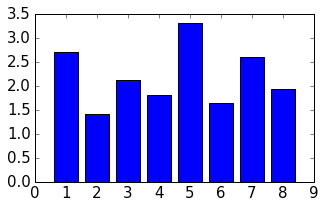
\includegraphics{8-Sensitivity-Analysis_26_1.png}

The previous experiment showed how \code{pynoddy} can be used for simple
scientific experiments. The sensitivity analysis itself is purely local.
A better way would be to use (more) global sensitivity analysis, for
example using the Morris or Sobol methods. These methods are implemented
in the Python package \code{SALib}, and an experimental implementation of
this method into \code{pynoddy} exists, as well (see further notebooks on
repository, note: no guaranteed working, so far!).


\chapter{Simulation of a Noddy history and analysis of its voxel topology}
\label{notebooks/9-Topology::doc}\label{notebooks/9-Topology:simulation-of-a-noddy-history-and-analysis-of-its-voxel-topology}
Example of how the module can be used to run Noddy simulations and
analyse the output.

\begin{Verbatim}[commandchars=\\\{\}]
\PYG{k+kn}{from} \PYG{n+nn}{IPython.core.display} \PYG{k+kn}{import} \PYG{n}{HTML}
\PYG{n}{css\PYGZus{}file} \PYG{o}{=} \PYG{l+s}{\PYGZsq{}}\PYG{l+s}{pynoddy.css}\PYG{l+s}{\PYGZsq{}}
\PYG{n}{HTML}\PYG{p}{(}\PYG{n+nb}{open}\PYG{p}{(}\PYG{n}{css\PYGZus{}file}\PYG{p}{,} \PYG{l+s}{\PYGZdq{}}\PYG{l+s}{r}\PYG{l+s}{\PYGZdq{}}\PYG{p}{)}\PYG{o}{.}\PYG{n}{read}\PYG{p}{(}\PYG{p}{)}\PYG{p}{)}
\end{Verbatim}
>>>>>>> refs/remotes/flohorovicic/master

\begin{Verbatim}[commandchars=\\\{\}]
\PYGZsh{} Basic settings
import sys, os
import subprocess

<<<<<<< HEAD
\index{swap\_events() (pynoddy.history.NoddyHistory method)}

\begin{fulllineitems}
\phantomsection\label{pynoddy:pynoddy.history.NoddyHistory.swap_events}\pysiglinewithargsret{\bfcode{swap\_events}}{\emph{event\_num\_1}, \emph{event\_num\_2}}{}
Swap two geological events in the timeline
\begin{description}
\item[{\textbf{Arguments}:}] \leavevmode\begin{itemize}
\item {} 
\emph{event\_num\_1/2} = int : number of events to be swapped (``order'')
=======
\PYGZsh{} Now import pynoddy
import pynoddy
\PYGZpc{}matplotlib inline

\PYGZsh{} determine path of repository to set paths corretly below

repo\PYGZus{}path = os.path.realpath(\PYGZsq{}../..\PYGZsq{})
\end{Verbatim}


\section{Compute the model}
\label{notebooks/9-Topology:compute-the-model}
The simplest way to perform the Noddy simulation through Python is
simply to call the executable. One way that should be fairly platform
independent is to use Python's own subprocess module:

\begin{Verbatim}[commandchars=\\\{\}]
\PYG{c}{\PYGZsh{} Change to sandbox directory to store results}
\PYG{n}{os}\PYG{o}{.}\PYG{n}{chdir}\PYG{p}{(}\PYG{n}{os}\PYG{o}{.}\PYG{n}{path}\PYG{o}{.}\PYG{n}{join}\PYG{p}{(}\PYG{n}{repo\PYGZus{}path}\PYG{p}{,} \PYG{l+s}{\PYGZsq{}}\PYG{l+s}{sandbox}\PYG{l+s}{\PYGZsq{}}\PYG{p}{)}\PYG{p}{)}

\PYG{c}{\PYGZsh{} Path to exmaple directory in this repository}
\PYG{n}{example\PYGZus{}directory} \PYG{o}{=} \PYG{n}{os}\PYG{o}{.}\PYG{n}{path}\PYG{o}{.}\PYG{n}{join}\PYG{p}{(}\PYG{n}{repo\PYGZus{}path}\PYG{p}{,}\PYG{l+s}{\PYGZsq{}}\PYG{l+s}{examples}\PYG{l+s}{\PYGZsq{}}\PYG{p}{)}
\PYG{c}{\PYGZsh{} Compute noddy model for history file}
\PYG{n}{history\PYGZus{}file} \PYG{o}{=} \PYG{l+s}{\PYGZsq{}}\PYG{l+s}{strike\PYGZus{}slip.his}\PYG{l+s}{\PYGZsq{}}
\PYG{n}{history} \PYG{o}{=} \PYG{n}{os}\PYG{o}{.}\PYG{n}{path}\PYG{o}{.}\PYG{n}{join}\PYG{p}{(}\PYG{n}{example\PYGZus{}directory}\PYG{p}{,} \PYG{n}{history\PYGZus{}file}\PYG{p}{)}
\PYG{n}{nfiles} \PYG{o}{=} \PYG{l+m+mi}{1}
\PYG{n}{files} \PYG{o}{=} \PYG{l+s}{\PYGZsq{}}\PYG{l+s}{\PYGZus{}}\PYG{l+s}{\PYGZsq{}}\PYG{o}{+}\PYG{n+nb}{str}\PYG{p}{(}\PYG{n}{nfiles}\PYG{p}{)}\PYG{o}{.}\PYG{n}{zfill}\PYG{p}{(}\PYG{l+m+mi}{4}\PYG{p}{)}
\PYG{k}{print} \PYG{l+s}{\PYGZdq{}}\PYG{l+s}{files}\PYG{l+s}{\PYGZdq{}}\PYG{p}{,} \PYG{n}{files}
\PYG{n}{root\PYGZus{}name} \PYG{o}{=} \PYG{l+s}{\PYGZsq{}}\PYG{l+s}{noddy\PYGZus{}out}\PYG{l+s}{\PYGZsq{}}
\PYG{n}{output\PYGZus{}name} \PYG{o}{=} \PYG{n}{root\PYGZus{}name} \PYG{o}{+} \PYG{n}{files}
\PYG{k}{print} \PYG{n}{root\PYGZus{}name}
\PYG{k}{print} \PYG{n}{output\PYGZus{}name}
\PYG{c}{\PYGZsh{} call Noddy}

\PYG{c}{\PYGZsh{} NOTE: Make sure that the noddy executable is accessible in the system!!}
\PYG{n}{sys}
\PYG{k}{print} \PYG{n}{subprocess}\PYG{o}{.}\PYG{n}{Popen}\PYG{p}{(}\PYG{p}{[}\PYG{l+s}{\PYGZsq{}}\PYG{l+s}{noddy.exe}\PYG{l+s}{\PYGZsq{}}\PYG{p}{,} \PYG{n}{history}\PYG{p}{,} \PYG{n}{output\PYGZus{}name}\PYG{p}{,} \PYG{l+s}{\PYGZsq{}}\PYG{l+s}{TOPOLOGY}\PYG{l+s}{\PYGZsq{}}\PYG{p}{]}\PYG{p}{,}
                       \PYG{n}{shell}\PYG{o}{=}\PYG{n+nb+bp}{False}\PYG{p}{,} \PYG{n}{stderr}\PYG{o}{=}\PYG{n}{subprocess}\PYG{o}{.}\PYG{n}{PIPE}\PYG{p}{,}
                       \PYG{n}{stdout}\PYG{o}{=}\PYG{n}{subprocess}\PYG{o}{.}\PYG{n}{PIPE}\PYG{p}{)}\PYG{o}{.}\PYG{n}{stdout}\PYG{o}{.}\PYG{n}{read}\PYG{p}{(}\PYG{p}{)}
\PYG{c}{\PYGZsh{}}
\PYG{n}{sys}
\PYG{k}{print} \PYG{n}{subprocess}\PYG{o}{.}\PYG{n}{Popen}\PYG{p}{(}\PYG{p}{[}\PYG{l+s}{\PYGZsq{}}\PYG{l+s}{topology.exe}\PYG{l+s}{\PYGZsq{}}\PYG{p}{,} \PYG{n}{root\PYGZus{}name}\PYG{p}{,} \PYG{n}{files}\PYG{p}{]}\PYG{p}{,}
                       \PYG{n}{shell}\PYG{o}{=}\PYG{n+nb+bp}{False}\PYG{p}{,} \PYG{n}{stderr}\PYG{o}{=}\PYG{n}{subprocess}\PYG{o}{.}\PYG{n}{PIPE}\PYG{p}{,}
                       \PYG{n}{stdout}\PYG{o}{=}\PYG{n}{subprocess}\PYG{o}{.}\PYG{n}{PIPE}\PYG{p}{)}\PYG{o}{.}\PYG{n}{stdout}\PYG{o}{.}\PYG{n}{read}\PYG{p}{(}\PYG{p}{)}
\end{Verbatim}

\begin{Verbatim}[commandchars=\\\{\}]
files \PYGZus{}0001
noddy\PYGZus{}out
noddy\PYGZus{}out\PYGZus{}0001
\end{Verbatim}
>>>>>>> refs/remotes/flohorovicic/master

For convenience, the model computations are wrapped into a Python
function in pynoddy:

\begin{Verbatim}[commandchars=\\\{\}]
\PYG{n}{pynoddy}\PYG{o}{.}\PYG{n}{compute\PYGZus{}model}\PYG{p}{(}\PYG{n}{history}\PYG{p}{,} \PYG{n}{output\PYGZus{}name}\PYG{p}{)}
\PYG{n}{pynoddy}\PYG{o}{.}\PYG{n}{compute\PYGZus{}topology}\PYG{p}{(}\PYG{n}{root\PYGZus{}name}\PYG{p}{,} \PYG{n}{files}\PYG{p}{)}
\end{Verbatim}

Note: The Noddy call from Python is, to date, calling Noddy through the
subprocess function. In a future implementation, this call could be
subsituted with a full wrapper for the C-functions written in Python.
Therefore, using the member function compute\_model is not only easier,
but also the more ``future-proof'' way to compute the Noddy model.

<<<<<<< HEAD
\index{update\_all\_event\_properties() (pynoddy.history.NoddyHistory method)}

\begin{fulllineitems}
\phantomsection\label{pynoddy:pynoddy.history.NoddyHistory.update_all_event_properties}\pysiglinewithargsret{\bfcode{update\_all\_event\_properties}}{}{}
Update properties of all events - in case changes were made
=======

\section{Loading Topology output files}
\label{notebooks/9-Topology:loading-topology-output-files}
Here we load the binary adjacency matrix for one topology calculation
and display it as an image
>>>>>>> refs/remotes/flohorovicic/master

\begin{Verbatim}[commandchars=\\\{\}]
\PYG{k+kn}{from} \PYG{n+nn}{matplotlib} \PYG{k+kn}{import} \PYG{n}{pyplot} \PYG{k}{as} \PYG{n}{plt}
\PYG{k+kn}{import} \PYG{n+nn}{matplotlib.image} \PYG{k+kn}{as} \PYG{n+nn}{mpimg}
\PYG{k+kn}{import} \PYG{n+nn}{numpy} \PYG{k+kn}{as} \PYG{n+nn}{np}

<<<<<<< HEAD
\index{update\_event\_numbers() (pynoddy.history.NoddyHistory method)}

\begin{fulllineitems}
\phantomsection\label{pynoddy:pynoddy.history.NoddyHistory.update_event_numbers}\pysiglinewithargsret{\bfcode{update\_event\_numbers}}{}{}
Update event numbers in `Event \#' line in noddy history file
=======
\PYG{n}{N1} \PYG{o}{=} \PYG{n}{pynoddy}\PYG{o}{.}\PYG{n}{NoddyOutput}\PYG{p}{(}\PYG{n}{output\PYGZus{}name}\PYG{p}{)}
\PYG{n}{AM}\PYG{o}{=} \PYG{n}{pynoddy}\PYG{o}{.}\PYG{n}{NoddyTopology}\PYG{p}{(}\PYG{n}{output\PYGZus{}name}\PYG{p}{)}

\PYG{n}{am\PYGZus{}name}\PYG{o}{=}\PYG{n}{root\PYGZus{}name} \PYG{o}{+}\PYG{l+s}{\PYGZsq{}}\PYG{l+s}{\PYGZus{}uam.bin}\PYG{l+s}{\PYGZsq{}}
\PYG{k}{print} \PYG{n}{am\PYGZus{}name}
\PYG{k}{print} \PYG{n}{AM}\PYG{o}{.}\PYG{n}{maxlitho}

\PYG{n}{image} \PYG{o}{=} \PYG{n}{np}\PYG{o}{.}\PYG{n}{empty}\PYG{p}{(}\PYG{p}{(}\PYG{n+nb}{int}\PYG{p}{(}\PYG{n}{AM}\PYG{o}{.}\PYG{n}{maxlitho}\PYG{p}{)}\PYG{p}{,}\PYG{n+nb}{int}\PYG{p}{(}\PYG{n}{AM}\PYG{o}{.}\PYG{n}{maxlitho}\PYG{p}{)}\PYG{p}{)}\PYG{p}{,} \PYG{n}{np}\PYG{o}{.}\PYG{n}{uint8}\PYG{p}{)}

\PYG{n}{image}\PYG{o}{.}\PYG{n}{data}\PYG{p}{[}\PYG{p}{:}\PYG{p}{]} \PYG{o}{=} \PYG{n+nb}{open}\PYG{p}{(}\PYG{n}{am\PYGZus{}name}\PYG{p}{)}\PYG{o}{.}\PYG{n}{read}\PYG{p}{(}\PYG{p}{)}
\PYG{n}{cmap}\PYG{o}{=}\PYG{n}{plt}\PYG{o}{.}\PYG{n}{get\PYGZus{}cmap}\PYG{p}{(}\PYG{l+s}{\PYGZsq{}}\PYG{l+s}{Paired}\PYG{l+s}{\PYGZsq{}}\PYG{p}{)}
\PYG{n}{cmap}\PYG{o}{.}\PYG{n}{set\PYGZus{}under}\PYG{p}{(}\PYG{l+s}{\PYGZsq{}}\PYG{l+s}{white}\PYG{l+s}{\PYGZsq{}}\PYG{p}{)}  \PYG{c}{\PYGZsh{} Color for values less than vmin}

\PYG{n}{plt}\PYG{o}{.}\PYG{n}{imshow}\PYG{p}{(}\PYG{n}{image}\PYG{p}{,} \PYG{n}{interpolation}\PYG{o}{=}\PYG{l+s}{\PYGZdq{}}\PYG{l+s}{nearest}\PYG{l+s}{\PYGZdq{}}\PYG{p}{,} \PYG{n}{vmin}\PYG{o}{=}\PYG{l+m+mi}{1}\PYG{p}{,} \PYG{n}{cmap}\PYG{o}{=}\PYG{n}{cmap}\PYG{p}{)}
\PYG{n}{plt}\PYG{o}{.}\PYG{n}{show}\PYG{p}{(}\PYG{p}{)}
\end{Verbatim}

\begin{Verbatim}[commandchars=\\\{\}]
\PYG{n}{maxlitho} \PYG{o}{=} \PYG{l+m+mi}{7}

\PYG{n}{noddy\PYGZus{}out\PYGZus{}uam}\PYG{o}{.}\PYG{n}{bin}
\PYG{l+m+mi}{7}
\end{Verbatim}
>>>>>>> refs/remotes/flohorovicic/master

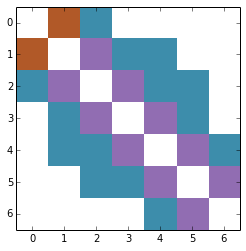
\includegraphics{9-Topology_9_1.png}

<<<<<<< HEAD
\index{write\_history() (pynoddy.history.NoddyHistory method)}

\begin{fulllineitems}
\phantomsection\label{pynoddy:pynoddy.history.NoddyHistory.write_history}\pysiglinewithargsret{\bfcode{write\_history}}{\emph{filename}}{}
Write history to new file
\begin{description}
\item[{\textbf{Arguments}:}] \leavevmode\begin{itemize}
\item {} 
\emph{filename} = string : filename of new history file
=======

\chapter{Fault shapes}
\label{notebooks/10-Fault-Shapes:fault-shapes}\label{notebooks/10-Fault-Shapes::doc}
We are here briefly showing the possibility of Noddy to model more
complex fault shapes than simple planar faults.

\begin{Verbatim}[commandchars=\\\{\}]
\PYG{k+kn}{from} \PYG{n+nn}{matplotlib} \PYG{k+kn}{import} \PYG{n}{rc\PYGZus{}params}
\end{Verbatim}
>>>>>>> refs/remotes/flohorovicic/master

\begin{Verbatim}[commandchars=\\\{\}]
\PYG{k+kn}{from} \PYG{n+nn}{IPython.core.display} \PYG{k+kn}{import} \PYG{n}{HTML}
\PYG{n}{css\PYGZus{}file} \PYG{o}{=} \PYG{l+s}{\PYGZsq{}}\PYG{l+s}{pynoddy.css}\PYG{l+s}{\PYGZsq{}}
\PYG{n}{HTML}\PYG{p}{(}\PYG{n+nb}{open}\PYG{p}{(}\PYG{n}{css\PYGZus{}file}\PYG{p}{,} \PYG{l+s}{\PYGZdq{}}\PYG{l+s}{r}\PYG{l+s}{\PYGZdq{}}\PYG{p}{)}\PYG{o}{.}\PYG{n}{read}\PYG{p}{(}\PYG{p}{)}\PYG{p}{)}
\end{Verbatim}

\begin{Verbatim}[commandchars=\\\{\}]
\PYG{k+kn}{import} \PYG{n+nn}{sys}\PYG{o}{,} \PYG{n+nn}{os}
\PYG{k+kn}{import} \PYG{n+nn}{matplotlib.pyplot} \PYG{k+kn}{as} \PYG{n+nn}{plt}
\PYG{c}{\PYGZsh{} adjust some settings for matplotlib}
\PYG{k+kn}{from} \PYG{n+nn}{matplotlib} \PYG{k+kn}{import} \PYG{n}{rcParams}
\PYG{c}{\PYGZsh{} print rcParams}
\PYG{n}{rcParams}\PYG{p}{[}\PYG{l+s}{\PYGZsq{}}\PYG{l+s}{font.size}\PYG{l+s}{\PYGZsq{}}\PYG{p}{]} \PYG{o}{=} \PYG{l+m+mi}{15}
\PYG{c}{\PYGZsh{} determine path of repository to set paths corretly below}
\PYG{n}{repo\PYGZus{}path} \PYG{o}{=} \PYG{n}{os}\PYG{o}{.}\PYG{n}{path}\PYG{o}{.}\PYG{n}{realpath}\PYG{p}{(}\PYG{l+s}{\PYGZsq{}}\PYG{l+s}{../..}\PYG{l+s}{\PYGZsq{}}\PYG{p}{)}
\PYG{k+kn}{import} \PYG{n+nn}{pynoddy.history}
\PYG{k+kn}{import} \PYG{n+nn}{pynoddy.experiment}
\PYG{k+kn}{import} \PYG{n+nn}{pynoddy.events}
\end{Verbatim}

<<<<<<< HEAD
\begin{notice}{hint}{Hint:}
Just love it how easy it is to `write history' with Noddy ;-)
\end{notice}
=======
\begin{Verbatim}[commandchars=\\\{\}]
\PYGZlt{}module \PYGZsq{}pynoddy.experiment\PYGZsq{} from \PYGZsq{}/Users/flow/git/pynoddy/pynoddy/experiment/\PYGZus{}\PYGZus{}init\PYGZus{}\PYGZus{}.pyc\PYGZsq{}\PYGZgt{}
\end{Verbatim}
>>>>>>> refs/remotes/flohorovicic/master

\begin{Verbatim}[commandchars=\\\{\}]
\PYGZpc{}matplotlib inline
\end{Verbatim}

<<<<<<< HEAD
=======
\begin{Verbatim}[commandchars=\\\{\}]
\PYG{n}{rcParams}\PYG{o}{.}\PYG{n}{update}\PYG{p}{(}\PYG{p}{\PYGZob{}}\PYG{l+s}{\PYGZsq{}}\PYG{l+s}{font.size}\PYG{l+s}{\PYGZsq{}}\PYG{p}{:} \PYG{l+m+mi}{20}\PYG{p}{\PYGZcb{}}\PYG{p}{)}
\end{Verbatim}

We will create a model with a listric fault from scratch. In addition to
the previous parameters for creating a fault (see notebook
4-Create-model), we now change the fault ``geometry'' to ``Curved'' and add
parameters defining the amplitude and radius of influence:

\begin{Verbatim}[commandchars=\\\{\}]
\PYG{n+nb}{reload}\PYG{p}{(}\PYG{n}{pynoddy}\PYG{o}{.}\PYG{n}{history}\PYG{p}{)}
\PYG{n+nb}{reload}\PYG{p}{(}\PYG{n}{pynoddy}\PYG{o}{.}\PYG{n}{events}\PYG{p}{)}
\PYG{n}{nm} \PYG{o}{=} \PYG{n}{pynoddy}\PYG{o}{.}\PYG{n}{history}\PYG{o}{.}\PYG{n}{NoddyHistory}\PYG{p}{(}\PYG{p}{)}
\PYG{c}{\PYGZsh{} add stratigraphy}
\PYG{n}{strati\PYGZus{}options} \PYG{o}{=} \PYG{p}{\PYGZob{}}\PYG{l+s}{\PYGZsq{}}\PYG{l+s}{num\PYGZus{}layers}\PYG{l+s}{\PYGZsq{}} \PYG{p}{:} \PYG{l+m+mi}{8}\PYG{p}{,}
                  \PYG{l+s}{\PYGZsq{}}\PYG{l+s}{layer\PYGZus{}names}\PYG{l+s}{\PYGZsq{}} \PYG{p}{:} \PYG{p}{[}\PYG{l+s}{\PYGZsq{}}\PYG{l+s}{layer 1}\PYG{l+s}{\PYGZsq{}}\PYG{p}{,} \PYG{l+s}{\PYGZsq{}}\PYG{l+s}{layer 2}\PYG{l+s}{\PYGZsq{}}\PYG{p}{,} \PYG{l+s}{\PYGZsq{}}\PYG{l+s}{layer 3}\PYG{l+s}{\PYGZsq{}}\PYG{p}{,} \PYG{l+s}{\PYGZsq{}}\PYG{l+s}{layer 4}\PYG{l+s}{\PYGZsq{}}\PYG{p}{,} \PYG{l+s}{\PYGZsq{}}\PYG{l+s}{layer 5}\PYG{l+s}{\PYGZsq{}}\PYG{p}{,} \PYG{l+s}{\PYGZsq{}}\PYG{l+s}{layer 6}\PYG{l+s}{\PYGZsq{}}\PYG{p}{,} \PYG{l+s}{\PYGZsq{}}\PYG{l+s}{layer 7}\PYG{l+s}{\PYGZsq{}}\PYG{p}{,} \PYG{l+s}{\PYGZsq{}}\PYG{l+s}{layer 8}\PYG{l+s}{\PYGZsq{}}\PYG{p}{]}\PYG{p}{,}
                  \PYG{l+s}{\PYGZsq{}}\PYG{l+s}{layer\PYGZus{}thickness}\PYG{l+s}{\PYGZsq{}} \PYG{p}{:} \PYG{p}{[}\PYG{l+m+mi}{1000}\PYG{p}{,} \PYG{l+m+mi}{500}\PYG{p}{,} \PYG{l+m+mi}{500}\PYG{p}{,} \PYG{l+m+mi}{500}\PYG{p}{,} \PYG{l+m+mi}{500}\PYG{p}{,} \PYG{l+m+mi}{500}\PYG{p}{,} \PYG{l+m+mi}{1000}\PYG{p}{,} \PYG{l+m+mi}{2000}\PYG{p}{]}\PYG{p}{\PYGZcb{}}
\PYG{n}{nm}\PYG{o}{.}\PYG{n}{add\PYGZus{}event}\PYG{p}{(}\PYG{l+s}{\PYGZsq{}}\PYG{l+s}{stratigraphy}\PYG{l+s}{\PYGZsq{}}\PYG{p}{,} \PYG{n}{strati\PYGZus{}options} \PYG{p}{)}

\PYG{c}{\PYGZsh{} The following options define the fault geometry:}
\PYG{n}{fault\PYGZus{}options} \PYG{o}{=} \PYG{p}{\PYGZob{}}\PYG{l+s}{\PYGZsq{}}\PYG{l+s}{name}\PYG{l+s}{\PYGZsq{}} \PYG{p}{:} \PYG{l+s}{\PYGZsq{}}\PYG{l+s}{Fault\PYGZus{}E}\PYG{l+s}{\PYGZsq{}}\PYG{p}{,}
                 \PYG{l+s}{\PYGZsq{}}\PYG{l+s}{pos}\PYG{l+s}{\PYGZsq{}} \PYG{p}{:} \PYG{p}{(}\PYG{l+m+mi}{3000}\PYG{p}{,} \PYG{l+m+mi}{0}\PYG{p}{,} \PYG{l+m+mi}{4000}\PYG{p}{)}\PYG{p}{,}
                 \PYG{l+s}{\PYGZsq{}}\PYG{l+s}{dip\PYGZus{}dir}\PYG{l+s}{\PYGZsq{}} \PYG{p}{:} \PYG{l+m+mi}{90}\PYG{p}{,}
                 \PYG{l+s}{\PYGZsq{}}\PYG{l+s}{dip}\PYG{l+s}{\PYGZsq{}} \PYG{p}{:} \PYG{l+m+mi}{30}\PYG{p}{,}
                 \PYG{l+s}{\PYGZsq{}}\PYG{l+s}{slip}\PYG{l+s}{\PYGZsq{}} \PYG{p}{:} \PYG{l+m+mi}{1000}\PYG{p}{,}
                 \PYG{l+s}{\PYGZsq{}}\PYG{l+s}{amplitude}\PYG{l+s}{\PYGZsq{}} \PYG{p}{:} \PYG{l+m+mf}{1000.}\PYG{p}{,}
                 \PYG{l+s}{\PYGZsq{}}\PYG{l+s}{radius}\PYG{l+s}{\PYGZsq{}} \PYG{p}{:} \PYG{l+m+mi}{2000}\PYG{p}{,}
                \PYG{l+s}{\PYGZsq{}}\PYG{l+s}{geometry}\PYG{l+s}{\PYGZsq{}} \PYG{p}{:} \PYG{l+s}{\PYGZsq{}}\PYG{l+s}{Curved}\PYG{l+s}{\PYGZsq{}}\PYG{p}{,}
                \PYG{l+s}{\PYGZsq{}}\PYG{l+s}{xaxis}\PYG{l+s}{\PYGZsq{}}\PYG{p}{:} \PYG{l+m+mf}{5000.}\PYG{p}{,}
                 \PYG{l+s}{\PYGZsq{}}\PYG{l+s}{yaxis}\PYG{l+s}{\PYGZsq{}}\PYG{p}{:} \PYG{l+m+mf}{5000.0}\PYG{p}{,}
                \PYG{l+s}{\PYGZsq{}}\PYG{l+s}{zaxis}\PYG{l+s}{\PYGZsq{}} \PYG{p}{:} \PYG{l+m+mf}{39999.0}\PYG{p}{\PYGZcb{}}
\PYG{n}{nm}\PYG{o}{.}\PYG{n}{add\PYGZus{}event}\PYG{p}{(}\PYG{l+s}{\PYGZsq{}}\PYG{l+s}{fault}\PYG{l+s}{\PYGZsq{}}\PYG{p}{,} \PYG{n}{fault\PYGZus{}options}\PYG{p}{)}
\PYG{n}{nm}\PYG{o}{.}\PYG{n}{change\PYGZus{}cube\PYGZus{}size}\PYG{p}{(}\PYG{l+m+mi}{50}\PYG{p}{)}
\end{Verbatim}
>>>>>>> refs/remotes/flohorovicic/master

With these settings, we obtain an example of a listric fault in Noddy:

<<<<<<< HEAD


\section{pynoddy.output module}
\label{pynoddy:module-pynoddy.output}\label{pynoddy:pynoddy-output-module}\index{pynoddy.output (module)}
Noddy output file analysis
Created on 24/03/2014

@author: Florian Wellmann
\index{NoddyOutput (class in pynoddy.output)}

\begin{fulllineitems}
\phantomsection\label{pynoddy:pynoddy.output.NoddyOutput}\pysiglinewithargsret{\strong{class }\code{pynoddy.output.}\bfcode{NoddyOutput}}{\emph{output\_name}}{}
Class definition for Noddy output analysis
\index{determine\_unit\_volumes() (pynoddy.output.NoddyOutput method)}

\begin{fulllineitems}
\phantomsection\label{pynoddy:pynoddy.output.NoddyOutput.determine_unit_volumes}\pysiglinewithargsret{\bfcode{determine\_unit\_volumes}}{}{}
Determine volumes of geological units in the discretized block model
=======
\begin{Verbatim}[commandchars=\\\{\}]
\PYG{n}{history} \PYG{o}{=} \PYG{l+s}{\PYGZdq{}}\PYG{l+s}{listric\PYGZus{}example.his}\PYG{l+s}{\PYGZdq{}}
\PYG{n}{outout\PYGZus{}name} \PYG{o}{=} \PYG{l+s}{\PYGZdq{}}\PYG{l+s}{listric\PYGZus{}out}\PYG{l+s}{\PYGZdq{}}

\PYG{n}{nm}\PYG{o}{.}\PYG{n}{write\PYGZus{}history}\PYG{p}{(}\PYG{n}{history}\PYG{p}{)}
\PYG{c}{\PYGZsh{} Compute the model}
\PYG{n}{pynoddy}\PYG{o}{.}\PYG{n}{compute\PYGZus{}model}\PYG{p}{(}\PYG{n}{history}\PYG{p}{,} \PYG{n}{output\PYGZus{}name}\PYG{p}{)}
\PYG{c}{\PYGZsh{} Plot output}
\PYG{n+nb}{reload}\PYG{p}{(}\PYG{n}{pynoddy}\PYG{o}{.}\PYG{n}{output}\PYG{p}{)}
\PYG{n}{nout} \PYG{o}{=} \PYG{n}{pynoddy}\PYG{o}{.}\PYG{n}{output}\PYG{o}{.}\PYG{n}{NoddyOutput}\PYG{p}{(}\PYG{n}{output\PYGZus{}name}\PYG{p}{)}
\PYG{n}{nout}\PYG{o}{.}\PYG{n}{plot\PYGZus{}section}\PYG{p}{(}\PYG{l+s}{\PYGZsq{}}\PYG{l+s}{y}\PYG{l+s}{\PYGZsq{}}\PYG{p}{,} \PYG{n}{layer\PYGZus{}labels} \PYG{o}{=} \PYG{n}{strati\PYGZus{}options}\PYG{p}{[}\PYG{l+s}{\PYGZsq{}}\PYG{l+s}{layer\PYGZus{}names}\PYG{l+s}{\PYGZsq{}}\PYG{p}{]}\PYG{p}{[}\PYG{p}{:}\PYG{p}{:}\PYG{o}{\PYGZhy{}}\PYG{l+m+mi}{1}\PYG{p}{]}\PYG{p}{,}
                  \PYG{n}{colorbar} \PYG{o}{=} \PYG{n+nb+bp}{True}\PYG{p}{,} \PYG{n}{title} \PYG{o}{=} \PYG{l+s}{\PYGZdq{}}\PYG{l+s}{\PYGZdq{}}\PYG{p}{,}
                  \PYG{n}{savefig} \PYG{o}{=} \PYG{n+nb+bp}{False}\PYG{p}{,} \PYG{n}{fig\PYGZus{}filename} \PYG{o}{=} \PYG{l+s}{\PYGZdq{}}\PYG{l+s}{ex01\PYGZus{}fault\PYGZus{}listric.eps}\PYG{l+s}{\PYGZdq{}}\PYG{p}{)}
\end{Verbatim}

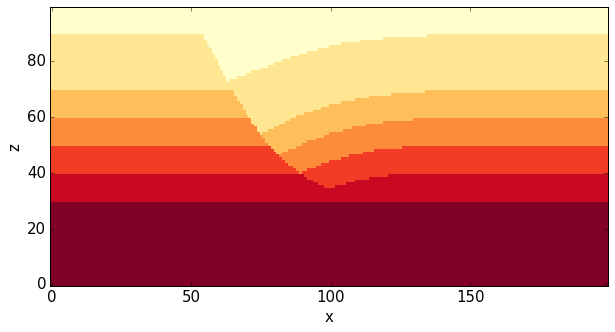
\includegraphics{10-Fault-Shapes_9_01.png}


\chapter{Pynoddy modules, classes and functions}
\label{pynoddy::doc}\label{pynoddy:pynoddy-modules-classes-and-functions}

\section{Basic modules (low-level access)}
\label{pynoddy:basic-modules-low-level-access}
The modules in this section provide low-level access to the functionality
in Noddy. Basically, these modules provide parsers for Noddy input and
output files and class definitions for suitable Noddy elements.
>>>>>>> refs/remotes/flohorovicic/master


<<<<<<< HEAD
\index{export\_to\_vtk() (pynoddy.output.NoddyOutput method)}

\begin{fulllineitems}
\phantomsection\label{pynoddy:pynoddy.output.NoddyOutput.export_to_vtk}\pysiglinewithargsret{\bfcode{export\_to\_vtk}}{\emph{**kwds}}{}
Export model to VTK

Export the geology blocks to VTK for visualisation of the entire 3-D model in an
external VTK viewer, e.g. Paraview.

..Note:: Requires pyevtk, available for free on: \href{https://github.com/firedrakeproject/firedrake/tree/master/python/evtk}{https://github.com/firedrakeproject/firedrake/tree/master/python/evtk}
=======
\subsection{Main module}
\label{pynoddy:main-module}\label{pynoddy:module-pynoddy}\index{pynoddy (module)}
Package initialization file for pynoddy
\index{compute\_model() (in module pynoddy)}

\begin{fulllineitems}
\phantomsection\label{pynoddy:pynoddy.compute_model}\pysiglinewithargsret{\code{pynoddy.}\bfcode{compute\_model}}{\emph{history}, \emph{output\_name}, \emph{**kwds}}{}
Call Noddy and compute the history file
>>>>>>> refs/remotes/flohorovicic/master
\begin{description}
\item[{\textbf{Arguments}:}] \leavevmode\begin{itemize}
\item {} 
<<<<<<< HEAD
\emph{vtk\_filename} = string : filename of VTK file (default: output\_name)

\end{itemize}

\end{description}

\end{fulllineitems}

\index{load\_geology() (pynoddy.output.NoddyOutput method)}

\begin{fulllineitems}
\phantomsection\label{pynoddy:pynoddy.output.NoddyOutput.load_geology}\pysiglinewithargsret{\bfcode{load\_geology}}{}{}
Load block geology ids from .g12 output file

\end{fulllineitems}

\index{load\_model\_info() (pynoddy.output.NoddyOutput method)}

\begin{fulllineitems}
\phantomsection\label{pynoddy:pynoddy.output.NoddyOutput.load_model_info}\pysiglinewithargsret{\bfcode{load\_model\_info}}{}{}
Load information about model discretisation from .g00 file
=======
\emph{history} = string : filename of history file

\item {} 
\emph{output\_name} = string : basename for output files

\end{itemize}

\item[{\textbf{Optional Keywords}:}] \leavevmode\begin{itemize}
\item {} 
\emph{sim\_type} = `BLOCK', `GEOPHYSICS', `SURFACES', `BLOCK\_GEOPHYS',

\end{itemize}
\begin{description}
\item[{`TOPOLOGY', `BLOCK\_SURFACES', `ALL':}] \leavevmode
type of Noddy simulation (default: `BLOCK')

\end{description}
\begin{itemize}
\item {} \begin{description}
\item[{\emph{program\_name} = string}] \leavevmode{[}name of program{]}
(default: noddy.exe or noddy, both checked)
>>>>>>> refs/remotes/flohorovicic/master

\end{description}

<<<<<<< HEAD
\index{plot\_section() (pynoddy.output.NoddyOutput method)}

\begin{fulllineitems}
\phantomsection\label{pynoddy:pynoddy.output.NoddyOutput.plot_section}\pysiglinewithargsret{\bfcode{plot\_section}}{\emph{direction='y'}, \emph{position='center'}, \emph{**kwds}}{}
Create a section block through the model
\begin{description}
\item[{\textbf{Arguments}:}] \leavevmode\begin{itemize}
\item {} 
\emph{direction} = `x', `y', `z' : coordinate direction of section plot (default: `y')
=======
\item {} 
\emph{verbose} = bool: verbose mode, print out information for debugging (default = False)

\item {} 
\emph{noddy\_path} = path: location of Noddy executable (default: checks environment variable)
>>>>>>> refs/remotes/flohorovicic/master

\item {} \begin{description}
\item[{\emph{position} = int or `center'}] \leavevmode{[}cell position of section as integer value{]}
or identifier (default: `center')

\item[{\textbf{Returns}:}] \leavevmode
-Returns any text outputted by the noddy executable.

\end{description}

<<<<<<< HEAD
=======
\end{fulllineitems}

\index{compute\_topology() (in module pynoddy)}

\begin{fulllineitems}
\phantomsection\label{pynoddy:pynoddy.compute_topology}\pysiglinewithargsret{\code{pynoddy.}\bfcode{compute\_topology}}{\emph{rootname}, \emph{**kwds}}{}
Call the topology executable to compute a models topology.
\begin{description}
\item[{\textbf{Arguments}:}] \leavevmode\begin{itemize}
\item {} 
\emph{rootname} = string : rootname of the noddy model to calculate topology for

>>>>>>> refs/remotes/flohorovicic/master
\end{itemize}

\item[{\textbf{Optional Keywords}:}] \leavevmode\begin{itemize}
\item {} 
<<<<<<< HEAD
\emph{ax} = matplotlib.axis : append plot to axis (default: create new plot)

\item {} 
\emph{figsize} = (x,y) : matplotlib figsize
=======
\emph{ensure\_discrete\_volumes} = True if topological units are broken down into
separate, spatially continuous volumes. Otherwise
some topological units may represent two separate
rock volumes (eg. if a folded unit has been truncated
by an unconformity). Default is True, though this is
a global variable (pynoddy.ensure\_discrete\_volumes)
so it can be changed during runtime.

\item {} 
\emph{null\_volume\_threshold} = The smallest non-null volume. volumes smaller than this are
ignored by the topology algorithm (as they represent pixelation artefacts).
The default is 20 voxels, though this is a global variable and can be changed
with pynoddy.null\_volume\_threshold.

\item {} 
\emph{topology\_path} = path: location of executable for topology calculation
>>>>>>> refs/remotes/flohorovicic/master

\item {} 
\emph{colorbar} = bool : plot colorbar (default: True)

<<<<<<< HEAD
\item {} 
\emph{title} = string : plot title
=======
\item[{\textbf{Returns}}] \leavevmode
-Returns any text outputted by the topology executable, including errors.

\end{description}
>>>>>>> refs/remotes/flohorovicic/master

\item {} 
\emph{savefig} = bool : save figure to file (default: show directly on screen)

<<<<<<< HEAD
\item {} 
\emph{cmap} = matplotlib.cmap : colormap

\item {} 
\emph{fig\_filename} = string : figure filename
=======
\index{which() (in module pynoddy)}

\begin{fulllineitems}
\phantomsection\label{pynoddy:pynoddy.which}\pysiglinewithargsret{\code{pynoddy.}\bfcode{which}}{\emph{program}}{}
\end{fulllineitems}
>>>>>>> refs/remotes/flohorovicic/master



\subsection{History file parser: pynoddy.history}
\label{pynoddy:module-pynoddy.history}\label{pynoddy:history-file-parser-pynoddy-history}\index{pynoddy.history (module)}
Noddy history file wrapper
Created on 24/03/2014

<<<<<<< HEAD

\end{fulllineitems}

=======
@author: Florian Wellmann
\index{NoddyHistory (class in pynoddy.history)}

\begin{fulllineitems}
\phantomsection\label{pynoddy:pynoddy.history.NoddyHistory}\pysiglinewithargsret{\strong{class }\code{pynoddy.history.}\bfcode{NoddyHistory}}{\emph{history=None}, \emph{**kwds}}{}
Bases: \code{object}

Class container for Noddy history files
\index{add\_event() (pynoddy.history.NoddyHistory method)}

\begin{fulllineitems}
\phantomsection\label{pynoddy:pynoddy.history.NoddyHistory.add_event}\pysiglinewithargsret{\bfcode{add\_event}}{\emph{event\_type}, \emph{event\_options}, \emph{**kwds}}{}
Add an event type to history
\begin{description}
\item[{\textbf{Arguments}:}] \leavevmode\begin{itemize}
\item {} 
\emph{event\_type} = string : type of event, legal options to date are:

\end{itemize}

`stratigraphy', `fault', `fold', `unconformity'
- \emph{event\_options} = list : required options to create event (event dependent)

\item[{\textbf{Optional keywords}:}] \leavevmode\begin{itemize}
\item {} 
\emph{event\_num} = int : event number (default: implicitly defined with increasing counter)
>>>>>>> refs/remotes/flohorovicic/master


\section{Module contents}
\label{pynoddy:module-contents}\label{pynoddy:module-pynoddy}\index{pynoddy (module)}
Package initialization file for pynoddy
\index{compute\_model() (in module pynoddy)}

\begin{fulllineitems}
\phantomsection\label{pynoddy:pynoddy.compute_model}\pysiglinewithargsret{\code{pynoddy.}\bfcode{compute\_model}}{\emph{history}, \emph{output\_name}}{}
\end{fulllineitems}

<<<<<<< HEAD


\chapter{Indices and tables}
\label{index:indices-and-tables}\begin{itemize}
\item {} 
\emph{genindex}

\item {} 
\emph{modindex}

\item {} 
\emph{search}

\end{itemize}

=======
\index{change\_cube\_size() (pynoddy.history.NoddyHistory method)}

\begin{fulllineitems}
\phantomsection\label{pynoddy:pynoddy.history.NoddyHistory.change_cube_size}\pysiglinewithargsret{\bfcode{change\_cube\_size}}{\emph{cube\_size}, \emph{**kwds}}{}
Change the model cube size (isotropic)
\begin{description}
\item[{\textbf{Arguments}:}] \leavevmode\begin{itemize}
\item {} 
\emph{cube\_size} = float : new model cube size

\end{itemize}

\end{description}

\end{fulllineitems}

\index{change\_event\_params() (pynoddy.history.NoddyHistory method)}

\begin{fulllineitems}
\phantomsection\label{pynoddy:pynoddy.history.NoddyHistory.change_event_params}\pysiglinewithargsret{\bfcode{change\_event\_params}}{\emph{changes\_dict}}{}
Change multiple event parameters according to settings in changes\_dict
\begin{description}
\item[{\textbf{Arguments}:}] \leavevmode\begin{itemize}
\item {} 
\emph{changes\_dict} = dictionary : entries define relative changes for (multiple) parameters

\end{itemize}

\end{description}

Per default, the values in the dictionary are added to the event parameters.

\end{fulllineitems}

\index{copy\_events() (pynoddy.history.NoddyHistory method)}

\begin{fulllineitems}
\phantomsection\label{pynoddy:pynoddy.history.NoddyHistory.copy_events}\pysiglinewithargsret{\bfcode{copy\_events}}{}{}
Create a copy of the current event state

\end{fulllineitems}

\index{create\_footer\_from\_template() (pynoddy.history.NoddyHistory method)}

\begin{fulllineitems}
\phantomsection\label{pynoddy:pynoddy.history.NoddyHistory.create_footer_from_template}\pysiglinewithargsret{\bfcode{create\_footer\_from\_template}}{}{}
Create model footer (with all settings) from template

\end{fulllineitems}

\index{create\_new\_history() (pynoddy.history.NoddyHistory method)}

\begin{fulllineitems}
\phantomsection\label{pynoddy:pynoddy.history.NoddyHistory.create_new_history}\pysiglinewithargsret{\bfcode{create\_new\_history}}{}{}
Methods to create a Noddy model

\end{fulllineitems}

\index{determine\_events() (pynoddy.history.NoddyHistory method)}

\begin{fulllineitems}
\phantomsection\label{pynoddy:pynoddy.history.NoddyHistory.determine_events}\pysiglinewithargsret{\bfcode{determine\_events}}{\emph{**kwds}}{}
Determine events and save line numbers

\begin{notice}{note}{Note:}\begin{description}
\item[{Parsing of the history file is based on a fixed Noddy output order. }] \leavevmode
If this is, for some reason (e.g. in a changed version of Noddy) not the case, then
this parsing might fail!

\item[{\textbf{Optional Keywords}:}] \leavevmode\begin{itemize}
\item {} 
verbose = True if this function is should write to the print bufffer, otherwise False. Default is False.

\end{itemize}

\end{description}
\end{notice}

\end{fulllineitems}

\index{determine\_model\_stratigraphy() (pynoddy.history.NoddyHistory method)}

\begin{fulllineitems}
\phantomsection\label{pynoddy:pynoddy.history.NoddyHistory.determine_model_stratigraphy}\pysiglinewithargsret{\bfcode{determine\_model\_stratigraphy}}{}{}
Determine stratigraphy of entire model from all events

\end{fulllineitems}

\index{get\_cube\_size() (pynoddy.history.NoddyHistory method)}

\begin{fulllineitems}
\phantomsection\label{pynoddy:pynoddy.history.NoddyHistory.get_cube_size}\pysiglinewithargsret{\bfcode{get\_cube\_size}}{\emph{**kwds}}{}
Determine cube size for model export
\textbf{Optional Args}
\begin{quote}

-type: choose geology or geophysics cube size to return. Should be either `Geology' (default) or `Geophysics'
\end{quote}

\end{fulllineitems}

\index{get\_date\_saved() (pynoddy.history.NoddyHistory method)}

\begin{fulllineitems}
\phantomsection\label{pynoddy:pynoddy.history.NoddyHistory.get_date_saved}\pysiglinewithargsret{\bfcode{get\_date\_saved}}{}{}
Determine the last savepoint of the file

\end{fulllineitems}

\index{get\_drillhole\_data() (pynoddy.history.NoddyHistory method)}

\begin{fulllineitems}
\phantomsection\label{pynoddy:pynoddy.history.NoddyHistory.get_drillhole_data}\pysiglinewithargsret{\bfcode{get\_drillhole\_data}}{\emph{x}, \emph{y}, \emph{**kwds}}{}
Get geology values along 1-D profile at position x,y with a 1 m resolution

The following steps are performed:
1. creates a copy of the entire object,
2. sets values of origin, extent and geology cube size, 
3. saves model to a temporary file, 
4. runs Noddy on that file
5. opens and analyses output
6. deletes temporary files

Note: this method only works if write access to current directory
is enabled and noddy can be executed!
\begin{description}
\item[{\textbf{Arguments}:}] \leavevmode\begin{itemize}
\item {} 
\emph{x} = float: x-position of drillhole

\item {} 
\emph{y} = float: y-position of drillhole

\end{itemize}

\item[{\textbf{Optional Arguments}:}] \leavevmode\begin{itemize}
\item {} 
\emph{z\_min} = float : minimum depth of drillhole (default: model range)

\item {} 
\emph{z\_max} = float : maximum depth of drillhole (default: model range)

\item {} 
\emph{resolution} = float : resolution along profile (default: 1 m)

\end{itemize}

\end{description}

\end{fulllineitems}

\index{get\_ev\_counter() (pynoddy.history.NoddyHistory method)}

\begin{fulllineitems}
\phantomsection\label{pynoddy:pynoddy.history.NoddyHistory.get_ev_counter}\pysiglinewithargsret{\bfcode{get\_ev\_counter}}{}{}
Event counter for implicit and continuous definition of events

\end{fulllineitems}

\index{get\_event\_param() (pynoddy.history.NoddyHistory method)}

\begin{fulllineitems}
\phantomsection\label{pynoddy:pynoddy.history.NoddyHistory.get_event_param}\pysiglinewithargsret{\bfcode{get\_event\_param}}{\emph{event\_number}, \emph{name}}{}
Returns the value of a given parameter for a given event.
\begin{description}
\item[{\textbf{Arguments}:}] \leavevmode\begin{itemize}
\item {} 
\emph{event\_number} = the event to get a parameter for (integer)

\item {} 
\emph{name} = the name of the parameter to retreive (string)

\end{itemize}
\begin{description}
\item[{\textbf{Returns}}] \leavevmode\begin{itemize}
\item {} 
Returns the value of the request parameter, or None if it does not 
exists.

\end{itemize}

\end{description}

\end{description}

\end{fulllineitems}

\index{get\_event\_params() (pynoddy.history.NoddyHistory method)}

\begin{fulllineitems}
\phantomsection\label{pynoddy:pynoddy.history.NoddyHistory.get_event_params}\pysiglinewithargsret{\bfcode{get\_event\_params}}{\emph{event\_number}}{}
Returns the parameter dictionary for a given event.
\begin{description}
\item[{\textbf{Arguments}:}] \leavevmode\begin{itemize}
\item {} 
\emph{event\_number} = the event to get a parameter for (integer)

\end{itemize}
\begin{description}
\item[{\textbf{Returns}}] \leavevmode\begin{itemize}
\item {} 
Returns the parameter dictionary for the requested event

\end{itemize}

\end{description}

\end{description}

\end{fulllineitems}

\index{get\_extent() (pynoddy.history.NoddyHistory method)}

\begin{fulllineitems}
\phantomsection\label{pynoddy:pynoddy.history.NoddyHistory.get_extent}\pysiglinewithargsret{\bfcode{get\_extent}}{}{}
Get model extent and return and store in local variables

\textbf{Returns}: (extent\_x, extent\_y, extent\_z)

\end{fulllineitems}

\index{get\_filename() (pynoddy.history.NoddyHistory method)}

\begin{fulllineitems}
\phantomsection\label{pynoddy:pynoddy.history.NoddyHistory.get_filename}\pysiglinewithargsret{\bfcode{get\_filename}}{}{}
Determine model filename from history file/ header

\end{fulllineitems}

\index{get\_footer\_lines() (pynoddy.history.NoddyHistory method)}

\begin{fulllineitems}
\phantomsection\label{pynoddy:pynoddy.history.NoddyHistory.get_footer_lines}\pysiglinewithargsret{\bfcode{get\_footer\_lines}}{}{}
Get the footer lines from self.history\_lines

The footer contains everything below events (all settings, etc.)

\end{fulllineitems}

\index{get\_info\_string() (pynoddy.history.NoddyHistory method)}

\begin{fulllineitems}
\phantomsection\label{pynoddy:pynoddy.history.NoddyHistory.get_info_string}\pysiglinewithargsret{\bfcode{get\_info\_string}}{\emph{**kwds}}{}
Get model information as string
\begin{description}
\item[{\textbf{Optional keywords}:}] \leavevmode\begin{itemize}
\item {} 
\emph{events\_only} = bool : only information on events

\end{itemize}

\end{description}

\end{fulllineitems}

\index{get\_origin() (pynoddy.history.NoddyHistory method)}

\begin{fulllineitems}
\phantomsection\label{pynoddy:pynoddy.history.NoddyHistory.get_origin}\pysiglinewithargsret{\bfcode{get\_origin}}{}{}
Get coordinates of model origin and return and store in local variables

\textbf{Returns}: (origin\_x, origin\_y, origin\_z)

\end{fulllineitems}

\index{info() (pynoddy.history.NoddyHistory method)}

\begin{fulllineitems}
\phantomsection\label{pynoddy:pynoddy.history.NoddyHistory.info}\pysiglinewithargsret{\bfcode{info}}{\emph{**kwds}}{}
Print out model information
\begin{description}
\item[{\textbf{Optional keywords}:}] \leavevmode\begin{itemize}
\item {} 
\emph{events\_only} = bool : only information on events

\end{itemize}

\end{description}

\end{fulllineitems}

\index{load\_history() (pynoddy.history.NoddyHistory method)}

\begin{fulllineitems}
\phantomsection\label{pynoddy:pynoddy.history.NoddyHistory.load_history}\pysiglinewithargsret{\bfcode{load\_history}}{\emph{history}}{}
Load Noddy history
\begin{description}
\item[{\textbf{Arguments}:}] \leavevmode\begin{itemize}
\item {} 
\emph{history} = string : Name of Noddy history file

\end{itemize}

\end{description}

\end{fulllineitems}

\index{load\_history\_from\_url() (pynoddy.history.NoddyHistory method)}

\begin{fulllineitems}
\phantomsection\label{pynoddy:pynoddy.history.NoddyHistory.load_history_from_url}\pysiglinewithargsret{\bfcode{load\_history\_from\_url}}{\emph{url}}{}
Directly load a Noddy history from a URL

This method is useful to load a model from the Structural Geophysics
Atlas on the pages of the Virtual Explorer.
See: \href{http://tectonique.net/asg}{http://tectonique.net/asg}
\begin{description}
\item[{\textbf{Arguments}:}] \leavevmode\begin{itemize}
\item {} 
\emph{url} : url of history file

\end{itemize}

\end{description}

\end{fulllineitems}

\index{reorder\_events() (pynoddy.history.NoddyHistory method)}

\begin{fulllineitems}
\phantomsection\label{pynoddy:pynoddy.history.NoddyHistory.reorder_events}\pysiglinewithargsret{\bfcode{reorder\_events}}{\emph{reorder\_dict}}{}
Reorder events accoring to assignment in reorder\_dict
\begin{description}
\item[{\textbf{Arguments}:}] \leavevmode\begin{itemize}
\item {} 
\emph{reorder\_dict} = dict : for example \{1 : 2, 2 : 3, 3 : 1\}

\end{itemize}

\end{description}

\end{fulllineitems}

\index{set\_event\_params() (pynoddy.history.NoddyHistory method)}

\begin{fulllineitems}
\phantomsection\label{pynoddy:pynoddy.history.NoddyHistory.set_event_params}\pysiglinewithargsret{\bfcode{set\_event\_params}}{\emph{params\_dict}}{}
set multiple event parameters according to settings in params\_dict
\begin{description}
\item[{\textbf{Arguments}:}] \leavevmode\begin{itemize}
\item {} 
\emph{params\_dict} = dictionary : entries to set (multiple) parameters

\end{itemize}

\end{description}

\end{fulllineitems}

\index{set\_extent() (pynoddy.history.NoddyHistory method)}

\begin{fulllineitems}
\phantomsection\label{pynoddy:pynoddy.history.NoddyHistory.set_extent}\pysiglinewithargsret{\bfcode{set\_extent}}{\emph{extent\_x}, \emph{extent\_y}, \emph{extent\_z}}{}
Set model extent and update local variables
\begin{description}
\item[{\textbf{Arguments}:}] \leavevmode\begin{itemize}
\item {} 
\emph{extent\_x} = float : extent in x-direction

\item {} 
\emph{extent\_y} = float : extent in y-direction

\item {} 
\emph{extent\_z} = float : extent in z-direction

\end{itemize}

\end{description}

\end{fulllineitems}

\index{set\_origin() (pynoddy.history.NoddyHistory method)}

\begin{fulllineitems}
\phantomsection\label{pynoddy:pynoddy.history.NoddyHistory.set_origin}\pysiglinewithargsret{\bfcode{set\_origin}}{\emph{origin\_x}, \emph{origin\_y}, \emph{origin\_z}}{}
Set coordinates of model origin and update local variables
\begin{description}
\item[{\textbf{Arguments}:}] \leavevmode\begin{itemize}
\item {} 
\emph{origin\_x} = float : x-location of model origin

\item {} 
\emph{origin\_y} = float : y-location of model origin

\item {} 
\emph{origin\_z} = float : z-location of model origin

\end{itemize}

\end{description}

\end{fulllineitems}

\index{swap\_events() (pynoddy.history.NoddyHistory method)}

\begin{fulllineitems}
\phantomsection\label{pynoddy:pynoddy.history.NoddyHistory.swap_events}\pysiglinewithargsret{\bfcode{swap\_events}}{\emph{event\_num\_1}, \emph{event\_num\_2}}{}
Swap two geological events in the timeline
\begin{description}
\item[{\textbf{Arguments}:}] \leavevmode\begin{itemize}
\item {} 
\emph{event\_num\_1/2} = int : number of events to be swapped (``order'')

\end{itemize}

\end{description}

\end{fulllineitems}

\index{update\_all\_event\_properties() (pynoddy.history.NoddyHistory method)}

\begin{fulllineitems}
\phantomsection\label{pynoddy:pynoddy.history.NoddyHistory.update_all_event_properties}\pysiglinewithargsret{\bfcode{update\_all\_event\_properties}}{}{}
Update properties of all events - in case changes were made

\end{fulllineitems}

\index{update\_event\_numbers() (pynoddy.history.NoddyHistory method)}

\begin{fulllineitems}
\phantomsection\label{pynoddy:pynoddy.history.NoddyHistory.update_event_numbers}\pysiglinewithargsret{\bfcode{update\_event\_numbers}}{}{}
Update event numbers in `Event \#' line in noddy history file

\end{fulllineitems}

\index{write\_history() (pynoddy.history.NoddyHistory method)}

\begin{fulllineitems}
\phantomsection\label{pynoddy:pynoddy.history.NoddyHistory.write_history}\pysiglinewithargsret{\bfcode{write\_history}}{\emph{filename}}{}
Write history to new file
\begin{description}
\item[{\textbf{Arguments}:}] \leavevmode\begin{itemize}
\item {} 
\emph{filename} = string : filename of new history file

\end{itemize}

\end{description}

\begin{notice}{hint}{Hint:}
Just love it how easy it is to `write history' with Noddy ;-)
\end{notice}

\end{fulllineitems}


\end{fulllineitems}



\subsection{Output file parser: pynoddy.output}
\label{pynoddy:module-pynoddy.output}\label{pynoddy:output-file-parser-pynoddy-output}\index{pynoddy.output (module)}
Noddy output file analysis
Created on 24/03/2014

@author: Florian Wellmann, Sam Thiele
\index{NoddyGeophysics (class in pynoddy.output)}

\begin{fulllineitems}
\phantomsection\label{pynoddy:pynoddy.output.NoddyGeophysics}\pysiglinewithargsret{\strong{class }\code{pynoddy.output.}\bfcode{NoddyGeophysics}}{\emph{output\_name}}{}
Bases: \code{object}

Definition to read, analyse, and visualise calculated geophysical responses
\index{read\_gravity() (pynoddy.output.NoddyGeophysics method)}

\begin{fulllineitems}
\phantomsection\label{pynoddy:pynoddy.output.NoddyGeophysics.read_gravity}\pysiglinewithargsret{\bfcode{read\_gravity}}{}{}
Read calculated gravity response

\end{fulllineitems}

\index{read\_magnetics() (pynoddy.output.NoddyGeophysics method)}

\begin{fulllineitems}
\phantomsection\label{pynoddy:pynoddy.output.NoddyGeophysics.read_magnetics}\pysiglinewithargsret{\bfcode{read\_magnetics}}{}{}
Read caluclated magnetic field response

\end{fulllineitems}


\end{fulllineitems}

\index{NoddyOutput (class in pynoddy.output)}

\begin{fulllineitems}
\phantomsection\label{pynoddy:pynoddy.output.NoddyOutput}\pysiglinewithargsret{\strong{class }\code{pynoddy.output.}\bfcode{NoddyOutput}}{\emph{output\_name}}{}
Bases: \code{object}

Class definition for Noddy output analysis
\index{compare\_dimensions\_to() (pynoddy.output.NoddyOutput method)}

\begin{fulllineitems}
\phantomsection\label{pynoddy:pynoddy.output.NoddyOutput.compare_dimensions_to}\pysiglinewithargsret{\bfcode{compare\_dimensions\_to}}{\emph{other}}{}
Compare model dimensions to another model

\end{fulllineitems}

\index{determine\_unit\_volumes() (pynoddy.output.NoddyOutput method)}

\begin{fulllineitems}
\phantomsection\label{pynoddy:pynoddy.output.NoddyOutput.determine_unit_volumes}\pysiglinewithargsret{\bfcode{determine\_unit\_volumes}}{}{}
Determine volumes of geological units in the discretized block model

\end{fulllineitems}

\index{export\_to\_vtk() (pynoddy.output.NoddyOutput method)}

\begin{fulllineitems}
\phantomsection\label{pynoddy:pynoddy.output.NoddyOutput.export_to_vtk}\pysiglinewithargsret{\bfcode{export\_to\_vtk}}{\emph{**kwds}}{}
Export model to VTK

Export the geology blocks to VTK for visualisation of the entire 3-D model in an
external VTK viewer, e.g. Paraview.

..Note:: Requires pyevtk, available for free on: \href{https://github.com/firedrakeproject/firedrake/tree/master/python/evtk}{https://github.com/firedrakeproject/firedrake/tree/master/python/evtk}
\begin{description}
\item[{\textbf{Optional keywords}:}] \leavevmode\begin{itemize}
\item {} 
\emph{vtk\_filename} = string : filename of VTK file (default: output\_name)

\item {} 
\emph{data} = np.array : data array to export to VKT (default: entire block model)

\end{itemize}

\end{description}

\end{fulllineitems}

\index{get\_section\_lines() (pynoddy.output.NoddyOutput method)}

\begin{fulllineitems}
\phantomsection\label{pynoddy:pynoddy.output.NoddyOutput.get_section_lines}\pysiglinewithargsret{\bfcode{get\_section\_lines}}{\emph{direction='y'}, \emph{position='center'}, \emph{**kwds}}{}
Create and returns a list of lines representing a section block through the model
\begin{description}
\item[{\textbf{Arguments}:}] \leavevmode\begin{itemize}
\item {} 
\emph{direction} = `x', `y', `z' : coordinate direction of section plot (default: `y')

\item {} \begin{description}
\item[{\emph{position} = int or `center'}] \leavevmode{[}cell position of section as integer value{]}
or identifier (default: `center')

\end{description}

\end{itemize}

\end{description}

\textbf{Returns}:
A tuple of lists of dictionaries.... ie:
( {[} dictionary of x coordinates, with lithology pairs as keys, separated by an underscore{]},
\begin{quote}

{[} dictionary of y coordinates, with lithology pairs as keys, separated by an underscore{]},
{[} dictionary of z coordinates, with lithology pairs as keys, separated by an underscore{]},
{[} dictionary of colours, with lithologies as keys{]})
\end{quote}

For example: get\_section\_lines(){[}0{]}{[}''1\_2''{]} returns a list of all the x coordinates from the 
contact between lithology 1 and lithology 2. Note that the smaller lithology index always
comes first in the code.

\end{fulllineitems}

\index{get\_section\_voxels() (pynoddy.output.NoddyOutput method)}

\begin{fulllineitems}
\phantomsection\label{pynoddy:pynoddy.output.NoddyOutput.get_section_voxels}\pysiglinewithargsret{\bfcode{get\_section\_voxels}}{\emph{direction='y'}, \emph{position='center'}, \emph{**kwds}}{}
Create and returns section block through the model
\begin{description}
\item[{\textbf{Arguments}:}] \leavevmode\begin{itemize}
\item {} 
\emph{direction} = `x', `y', `z' : coordinate direction of section plot (default: `y')

\item {} \begin{description}
\item[{\emph{position} = int or `center'}] \leavevmode{[}cell position of section as integer value{]}
or identifier (default: `center')

\end{description}

\end{itemize}

\item[{\textbf{Optional Keywords}:}] \leavevmode\begin{itemize}
\item {} 
\emph{data} = np.array : data to plot, if different to block data itself

\item {} 
\emph{litho\_filter} = a list of lithologies to draw. All others will be ignored.

\end{itemize}

\end{description}

\end{fulllineitems}

\index{get\_surface\_grid() (pynoddy.output.NoddyOutput method)}

\begin{fulllineitems}
\phantomsection\label{pynoddy:pynoddy.output.NoddyOutput.get_surface_grid}\pysiglinewithargsret{\bfcode{get\_surface\_grid}}{\emph{lithoID}, \emph{**kwds}}{}
Returns a grid of lines that define a grid on the specified surface. Note that this cannot
handle layers that are repeated in the z direction...
\begin{description}
\item[{\textbf{Arguments}:}] \leavevmode\begin{itemize}
\item {} \begin{description}
\item[{\emph{lithoID} - the top surface of this lithology will be calculated. If a list is passed,}] \leavevmode
the top surface of each lithology in the list is calculated.

\end{description}

\end{itemize}

\item[{\textbf{Keywords}:}] \leavevmode\begin{itemize}
\item {} 
\emph{res} - the resolution to sample at. Default is 2 (ie. every second voxel is sampled).

\end{itemize}

\item[{\textbf{Returns}:}] \leavevmode
a tuple containing lists of tuples of x, y and z coordinate dictionaries and colour dictionaries, 
one containing the east-west lines and one the north-south lines: ((x,y,z,c),(x,y,z,c)). THe dictionary
keys are the lithoID's passed in the lithoID parameter.

\end{description}

\end{fulllineitems}

\index{load\_geology() (pynoddy.output.NoddyOutput method)}

\begin{fulllineitems}
\phantomsection\label{pynoddy:pynoddy.output.NoddyOutput.load_geology}\pysiglinewithargsret{\bfcode{load\_geology}}{}{}
Load block geology ids from .g12 output file

\end{fulllineitems}

\index{load\_model\_info() (pynoddy.output.NoddyOutput method)}

\begin{fulllineitems}
\phantomsection\label{pynoddy:pynoddy.output.NoddyOutput.load_model_info}\pysiglinewithargsret{\bfcode{load\_model\_info}}{}{}
Load information about model discretisation from .g00 file

\end{fulllineitems}

\index{plot\_section() (pynoddy.output.NoddyOutput method)}

\begin{fulllineitems}
\phantomsection\label{pynoddy:pynoddy.output.NoddyOutput.plot_section}\pysiglinewithargsret{\bfcode{plot\_section}}{\emph{direction='y'}, \emph{position='center'}, \emph{**kwds}}{}
Create a section block through the model
\begin{description}
\item[{\textbf{Arguments}:}] \leavevmode\begin{itemize}
\item {} 
\emph{direction} = `x', `y', `z' : coordinate direction of section plot (default: `y')

\item {} \begin{description}
\item[{\emph{position} = int or `center'}] \leavevmode{[}cell position of section as integer value{]}
or identifier (default: `center')

\end{description}

\end{itemize}

\item[{\textbf{Optional Keywords}:}] \leavevmode\begin{itemize}
\item {} 
\emph{ax} = matplotlib.axis : append plot to axis (default: create new plot)

\item {} 
\emph{figsize} = (x,y) : matplotlib figsize

\item {} 
\emph{colorbar} = bool : plot colorbar (default: True)

\item {} \begin{description}
\item[{\emph{colorbar\_orientation} = `horizontal' or `vertical'}] \leavevmode{[}orientation of colorbar{]}
(default: `vertical')

\end{description}

\item {} 
\emph{title} = string : plot title

\item {} 
\emph{savefig} = bool : save figure to file (default: show directly on screen)

\item {} 
\emph{cmap} = matplotlib.cmap : colormap (default: YlOrRd)

\item {} 
\emph{fig\_filename} = string : figure filename

\item {} 
\emph{ve} = float : vertical exaggeration

\item {} 
\emph{layer\_labels} = list of strings: labels for each unit in plot

\item {} 
\emph{layers\_from} = noddy history file : get labels automatically from history file

\item {} 
\emph{data} = np.array : data to plot, if different to block data itself

\item {} 
\emph{litho\_filter} = a list of lithologies to draw. All others will be ignored.

\end{itemize}

\end{description}

\end{fulllineitems}

\index{set\_basename() (pynoddy.output.NoddyOutput method)}

\begin{fulllineitems}
\phantomsection\label{pynoddy:pynoddy.output.NoddyOutput.set_basename}\pysiglinewithargsret{\bfcode{set\_basename}}{\emph{name}}{}
Set model basename

\end{fulllineitems}


\end{fulllineitems}

\index{NoddyTopology (class in pynoddy.output)}

\begin{fulllineitems}
\phantomsection\label{pynoddy:pynoddy.output.NoddyTopology}\pysiglinewithargsret{\strong{class }\code{pynoddy.output.}\bfcode{NoddyTopology}}{\emph{noddy\_model}, \emph{**kwds}}{}
Bases: \code{object}

Definition to read, analyse, and visualise calculated voxel topology
\index{calculate\_difference() (pynoddy.output.NoddyTopology method)}

\begin{fulllineitems}
\phantomsection\label{pynoddy:pynoddy.output.NoddyTopology.calculate_difference}\pysiglinewithargsret{\bfcode{calculate\_difference}}{\emph{G2}, \emph{data=False}}{}
Calculates the difference between this NoddyTopology and another NoddyTopology or networkX graph
\begin{description}
\item[{\textbf{Arguments}}] \leavevmode\begin{itemize}
\item {} 
\emph{G2} = a valid NoddyTopology object or NetworkX graph that this topology is to be compared with

\end{itemize}

\item[{\textbf{Returns}}] \leavevmode
A tuple containing:
- The number of different edges 
- a list of these edges

\end{description}

\end{fulllineitems}

\index{calculate\_overlap() (pynoddy.output.NoddyTopology method)}

\begin{fulllineitems}
\phantomsection\label{pynoddy:pynoddy.output.NoddyTopology.calculate_overlap}\pysiglinewithargsret{\bfcode{calculate\_overlap}}{\emph{G2}}{}
Calculates the overlap between this NoddyTopology and another NoddyTopology or networkX graph
\begin{description}
\item[{\textbf{Arguments}}] \leavevmode\begin{itemize}
\item {} 
\emph{G2} = a valid NoddyTopology object or NetworkX graph that this topology is to be compared with

\end{itemize}

\item[{\textbf{Returns}}] \leavevmode\begin{itemize}
\item {} 
The number of overlapping edges

\item {} 
A list of these edges

\end{itemize}

\end{description}

\end{fulllineitems}

\index{calculate\_unique\_topologies() (pynoddy.output.NoddyTopology static method)}

\begin{fulllineitems}
\phantomsection\label{pynoddy:pynoddy.output.NoddyTopology.calculate_unique_topologies}\pysiglinewithargsret{\strong{static }\bfcode{calculate\_unique\_topologies}}{\emph{topology\_list}, \emph{**kwds}}{}
Calculates the number of unique topologies in a list of NoddyTopologies
\begin{description}
\item[{\textbf{Arguments}:}] \leavevmode\begin{itemize}
\item {} 
\emph{topology\_list} = The list of NoddyTopologies to search through.

\end{itemize}

\item[{\textbf{Optional Keywords}:}] \leavevmode\begin{itemize}
\item {} 
\emph{output} = A File or list to write cumulative observed topologies distribution. Default is None (nothing written).

\item {} 
\emph{ids} = A list to write the unique topology id's for each topology in the provided topology\_list (in that 
order). Default is None.

\item {} 
\emph{frequency} = A list to write frequency counts to.

\end{itemize}

\item[{\textbf{Returns}:}] \leavevmode\begin{itemize}
\item {} 
Returns a list of unique topologies.

\end{itemize}

\end{description}

\end{fulllineitems}

\index{collapse\_stratigraphy() (pynoddy.output.NoddyTopology method)}

\begin{fulllineitems}
\phantomsection\label{pynoddy:pynoddy.output.NoddyTopology.collapse_stratigraphy}\pysiglinewithargsret{\bfcode{collapse\_stratigraphy}}{}{}
Collapses all stratigraphic edges in this network to produce a network that only contains
structurally bound rock volumes. Essentially this is a network built only with Topology codes
and ignoring lithology
\begin{description}
\item[{\textbf{Returns}}] \leavevmode\begin{itemize}
\item {} 
a new NoddyTopology object containing the collapsed graph. The original object is not modified.

\end{itemize}

\end{description}

\end{fulllineitems}

\index{collapse\_structure() (pynoddy.output.NoddyTopology method)}

\begin{fulllineitems}
\phantomsection\label{pynoddy:pynoddy.output.NoddyTopology.collapse_structure}\pysiglinewithargsret{\bfcode{collapse\_structure}}{\emph{verbose=False}}{}
Collapses all topology codes down to the last (most recent) difference. Information regarding specific model topology is 
generalised, eg. lithology A has a fault and stratigrappic contact with B (regardless of how many different faults are involved).
\begin{description}
\item[{\textbf{Optional Arguments}:}] \leavevmode\begin{itemize}
\item {} 
\emph{verbose} = True if this function should write to the print buffer. Default is False.

\end{itemize}

\item[{\textbf{Returns}}] \leavevmode\begin{itemize}
\item {} 
a new NoddyTopology object containing the collapsed graph. The original object is not modified.

\end{itemize}

\end{description}

\end{fulllineitems}

\index{combine\_topologies() (pynoddy.output.NoddyTopology static method)}

\begin{fulllineitems}
\phantomsection\label{pynoddy:pynoddy.output.NoddyTopology.combine_topologies}\pysiglinewithargsret{\strong{static }\bfcode{combine\_topologies}}{\emph{topology\_list}}{}
Combines a list of topology networks into a weighted `super-network'. This is designed for
estimating the likelyhood of a given edge occuring using a series of networks generated in
a Monte-Carlo type analysis.
\begin{description}
\item[{\textbf{Arguments}}] \leavevmode\begin{itemize}
\item {} 
\emph{topology\_list} = A list of networkX graphs or NoddyTopology objects to build supernetwork from.

\end{itemize}

\item[{\textbf{Returns}}] \leavevmode\begin{itemize}
\item {} 
A NetworkX graph object containing all edges from the input graphs and weighted (`weight' parameter)
according to their observed frequency.

\end{itemize}

\end{description}

\end{fulllineitems}

\index{draw\_3d\_network() (pynoddy.output.NoddyTopology method)}

\begin{fulllineitems}
\phantomsection\label{pynoddy:pynoddy.output.NoddyTopology.draw_3d_network}\pysiglinewithargsret{\bfcode{draw\_3d\_network}}{\emph{**kwds}}{}
Draws a 3D network using matplotlib.
\begin{description}
\item[{\textbf{Optional Keywords}:}] \leavevmode\begin{itemize}
\item {} 
\emph{show} = If True, the 3D network is displayed immediatly on-screen in an interactive matplotlib viewer. Default is True.

\item {} 
\emph{output} = If defined an image of the network is saved to this location.

\item {} 
\emph{node\_size} = The size of the nodes. Default is 40.

\item {} 
\emph{geology} = a NoddyOutput object to draw with the network

\item {} 
\emph{res} = resolution to draw geology at. Default is 4 (ie 1/4 of all voxels are drawn)

\item {} 
\emph{horizons} = a list of geology surfaces to draw. Default is nothing (none drawn). Slow!
See NoddyOutput.get\_surface\_grid for details.

\item {} 
\emph{sections} = draw geology sections. Default is True.

\end{itemize}

\end{description}

\end{fulllineitems}

\index{draw\_adjacency\_matrix() (pynoddy.output.NoddyTopology method)}

\begin{fulllineitems}
\phantomsection\label{pynoddy:pynoddy.output.NoddyTopology.draw_adjacency_matrix}\pysiglinewithargsret{\bfcode{draw\_adjacency\_matrix}}{\emph{**kwds}}{}
Draws an adjacency matrix representing this topology object.
\begin{description}
\item[{\textbf{Keywords}:}] \leavevmode\begin{itemize}
\item {} 
\emph{path} = The path to save this image to. If not provided, the image is drawn to the screen

\item {} 
\emph{dpi} = The resolution to save this image. Default is 300

\item {} 
\emph{size} = The size of the image to save (in inches). This value will be used as the width and the height

\end{itemize}

\end{description}

\end{fulllineitems}

\index{draw\_difference\_matrix() (pynoddy.output.NoddyTopology method)}

\begin{fulllineitems}
\phantomsection\label{pynoddy:pynoddy.output.NoddyTopology.draw_difference_matrix}\pysiglinewithargsret{\bfcode{draw\_difference\_matrix}}{\emph{G2}, \emph{**kwds}}{}
Draws an adjacency matrix containing the difference between this topology and the provided topology
\begin{description}
\item[{\textbf{Arguments}:}] \leavevmode\begin{itemize}
\item {} 
\emph{G2} = A different NoddyTopology or NetworkX Graph to compare to

\end{itemize}

\item[{\textbf{Optional Keywords}:}] \leavevmode\begin{itemize}
\item {} 
\emph{strat} = A dictionary linking node names to stratigraphic heights and names. Should be as follows \{ node\_name : (height,name) \}.

\item {} 
\emph{path} = The path to save this image to. If not provided, the image is drawn to the screen

\item {} 
\emph{dpi} = The resolution to save this image. Default is 300

\item {} 
\emph{size} = The size of the image to save (in inches). This value will be used as the width and the height

\end{itemize}

\end{description}

\end{fulllineitems}

\index{draw\_graph\_matrix() (pynoddy.output.NoddyTopology static method)}

\begin{fulllineitems}
\phantomsection\label{pynoddy:pynoddy.output.NoddyTopology.draw_graph_matrix}\pysiglinewithargsret{\strong{static }\bfcode{draw\_graph\_matrix}}{\emph{G}, \emph{**kwds}}{}
Draws an adjacency matrix representing the specified graph object. Equivalent to
NoddyTopology.draw\_matrix\_image() but for a networkX graph object.
\begin{description}
\item[{\textbf{Keywords}:}] \leavevmode\begin{itemize}
\item {} 
\emph{strat} = A dictionary linking node names to stratigraphic heights and names. Should be as follows \{ node\_name : (height,name) \}.

\item {} 
\emph{path} = The path to save this image to. If not provided, the image is drawn to the screen

\item {} 
\emph{dpi} = The resolution to save this image. Default is 300

\item {} 
\emph{size} = The size of the image to save (in inches). This value will be used as the width and the height

\end{itemize}

\end{description}

\end{fulllineitems}

\index{draw\_mayavi() (pynoddy.output.NoddyTopology method)}

\begin{fulllineitems}
\phantomsection\label{pynoddy:pynoddy.output.NoddyTopology.draw_mayavi}\pysiglinewithargsret{\bfcode{draw\_mayavi}}{\emph{**kwds}}{}
Draws this network with mayavi. This requires the Mayavi python library
(mayavi.mlab)
\begin{description}
\item[{\textbf{Optional Keywords}:}] \leavevmode\begin{itemize}
\item {} 
\emph{node\_size} = The size of the nodes. Default is 40.

\item {} 
\emph{edge\_thickness} = The thickness of the edges. Default is 4

\item {} 
\emph{show} = If true, the model is displayed in the mayavi viewer after exporting. Default is True

\item {} 
\emph{path} = A path to save the mayavi vtk file to after generating it.

\end{itemize}

\end{description}

\end{fulllineitems}

\index{draw\_mayavi\_graph() (pynoddy.output.NoddyTopology static method)}

\begin{fulllineitems}
\phantomsection\label{pynoddy:pynoddy.output.NoddyTopology.draw_mayavi_graph}\pysiglinewithargsret{\strong{static }\bfcode{draw\_mayavi\_graph}}{\emph{G}, \emph{**kwds}}{}
Draws the provided network with mayavi. This requires the Mayavi python library
(mayavi.mlab)
\begin{description}
\item[{\textbf{Optional Keywords}:}] \leavevmode\begin{itemize}
\item {} 
\emph{node\_size} = The size of the nodes. Default is 40.

\item {} 
\emph{edge\_thickness} = The thickness of the edges. Default is 4

\item {} 
\emph{show} = If true, the model is displayed in the mayavi viewer after exporting. Default is True

\item {} 
\emph{path} = A path to save the mayavi vtk file to after generating it.

\end{itemize}

\end{description}

\end{fulllineitems}

\index{draw\_network\_hive() (pynoddy.output.NoddyTopology method)}

\begin{fulllineitems}
\phantomsection\label{pynoddy:pynoddy.output.NoddyTopology.draw_network_hive}\pysiglinewithargsret{\bfcode{draw\_network\_hive}}{\emph{**kwds}}{}
Draws a network hive plot (see \href{https://github.com/ericmjl/hiveplot}{https://github.com/ericmjl/hiveplot}).
The axes of the hive are: node lithology, edge age \& edge area.

ie. the top axis lists the nodes in stratigraphic order. The second axis
lists edges in structural age \& thrid axis lists edges by surface area.

Nodes are joined to edge-nodes by lines on the graph if they are topologically linked
(ie. if an edge has that node as an end point).
\begin{description}
\item[{\textbf{Optional Keywords}:}] \leavevmode\begin{itemize}
\item {} 
\emph{path} = the path to save this figure

\item {} 
\emph{dpi} = the resolution of the figure

\item {} 
\emph{bg} = the background color. Default is black.

\item {} 
\emph{axes} = The color of the axes and labels.

\end{itemize}

\end{description}

\end{fulllineitems}

\index{draw\_network\_image() (pynoddy.output.NoddyTopology method)}

\begin{fulllineitems}
\phantomsection\label{pynoddy:pynoddy.output.NoddyTopology.draw_network_image}\pysiglinewithargsret{\bfcode{draw\_network\_image}}{\emph{outputname='`}, \emph{**kwds}}{}
Draws a network diagram of this NoddyTopology to the specified image
\begin{description}
\item[{\textbf{Arguments}:}] \leavevmode\begin{itemize}
\item {} 
\emph{outputname} = the path of the image being written. If left as `' the image is written to the same directory as the basename.

\end{itemize}

\item[{\textbf{Optional Keywords}:}] \leavevmode\begin{itemize}
\item {} 
\emph{dimension} = `2D' for a 2D network diagram or `3D' for a 3D network diagram. Default is `2D'.

\item {} 
\emph{axis} = the axis to view on for 3D network diagrams

\item {} 
\emph{perspective} = True to use perspective projection, or False for orthographic projection. Default is False.

\item {} 
\emph{node\_size} = The size that nodes are drawn. Default is 1500.

\item {} 
\emph{layout} = The layout algorithm used in 2D. Options are `spring\_layout' (default), `shell\_layout', `circular\_layout' and `spectral\_layout'.

\item {} 
\emph{verbose} = True if this function is allowed to write to the print buffer, otherwise false. Default is False.

\end{itemize}

\end{description}

\end{fulllineitems}

\index{filter\_node\_volumes() (pynoddy.output.NoddyTopology method)}

\begin{fulllineitems}
\phantomsection\label{pynoddy:pynoddy.output.NoddyTopology.filter_node_volumes}\pysiglinewithargsret{\bfcode{filter\_node\_volumes}}{\emph{min\_volume=50}}{}
Removes all nodes with volumes less than the specified size
\begin{description}
\item[{\textbf{Arguments}:}] \leavevmode\begin{itemize}
\item {} 
\emph{min\_volume} = the threshold volume. Nodes with smaller volumes are deleted.

\end{itemize}

\item[{\textbf{Returns}}] \leavevmode\begin{itemize}
\item {} 
returns the number of deleted nodes

\end{itemize}

\end{description}

\end{fulllineitems}

\index{find\_first\_match() (pynoddy.output.NoddyTopology method)}

\begin{fulllineitems}
\phantomsection\label{pynoddy:pynoddy.output.NoddyTopology.find_first_match}\pysiglinewithargsret{\bfcode{find\_first\_match}}{\emph{known}}{}
Identical to is\_unique, except that the index of the first match is returned if this matches, otherwise
-1 is returned.
\begin{description}
\item[{\textbf{Arguments}:}] \leavevmode
-\emph{known} = a list of valid NoddyTopology objects or NetworkX graphs to compare with.

\item[{\textbf{Returns}:}] \leavevmode\begin{itemize}
\item {} 
Returns the index of the first matching topology object, or -1

\end{itemize}

\end{description}

\end{fulllineitems}

\index{find\_matching() (pynoddy.output.NoddyTopology method)}

\begin{fulllineitems}
\phantomsection\label{pynoddy:pynoddy.output.NoddyTopology.find_matching}\pysiglinewithargsret{\bfcode{find\_matching}}{\emph{known}}{}
Finds the first matching NoddyTopology (or NetworkX graph) in the specified list
\begin{description}
\item[{\textbf{Arguments}:}] \leavevmode
-\emph{known} = a list of valid NoddyTopology objects or NetworkX graphs to compare with.

\item[{\textbf{Returns}:}] \leavevmode\begin{itemize}
\item {} 
Returns the first matching object (jaccard coefficient = 1), or otherwise None

\end{itemize}

\end{description}

\end{fulllineitems}

\index{is\_unique() (pynoddy.output.NoddyTopology method)}

\begin{fulllineitems}
\phantomsection\label{pynoddy:pynoddy.output.NoddyTopology.is_unique}\pysiglinewithargsret{\bfcode{is\_unique}}{\emph{known}}{}
Returns True if the topology of this model is different (ie. forms a different network) to a list of models.
\begin{description}
\item[{\textbf{Arguments}:}] \leavevmode
-\emph{known} = a list of valid NoddyTopology objects or NetworkX graphs to compare with.

\item[{\textbf{Returns}:}] \leavevmode\begin{itemize}
\item {} 
Returns true if this topology is unique, otherwise false

\end{itemize}

\end{description}

\end{fulllineitems}

\index{jaccard\_coefficient() (pynoddy.output.NoddyTopology method)}

\begin{fulllineitems}
\phantomsection\label{pynoddy:pynoddy.output.NoddyTopology.jaccard_coefficient}\pysiglinewithargsret{\bfcode{jaccard\_coefficient}}{\emph{G2}}{}
Calculates the Jaccard Coefficient (ratio between the intersection \& union) of the graph representing this NOddyTopology and G2.
\begin{description}
\item[{\textbf{Arguments}}] \leavevmode\begin{itemize}
\item {} 
\emph{G2} = a valid NoddyTopology object or NetworkX graph that this topology is to be compared with

\end{itemize}

\item[{\textbf{Returns}}] \leavevmode\begin{itemize}
\item {} 
The jaccard\_coefficient

\end{itemize}

\end{description}

\end{fulllineitems}

\index{loadNetwork() (pynoddy.output.NoddyTopology method)}

\begin{fulllineitems}
\phantomsection\label{pynoddy:pynoddy.output.NoddyTopology.loadNetwork}\pysiglinewithargsret{\bfcode{loadNetwork}}{}{}
Loads the topology network into a NetworkX datastructure

\end{fulllineitems}

\index{read\_adjacency\_matrix() (pynoddy.output.NoddyTopology method)}

\begin{fulllineitems}
\phantomsection\label{pynoddy:pynoddy.output.NoddyTopology.read_adjacency_matrix}\pysiglinewithargsret{\bfcode{read\_adjacency\_matrix}}{}{}
\emph{Depreciated}
Reads max number of lithologies aross all models

\end{fulllineitems}

\index{read\_properties() (pynoddy.output.NoddyTopology method)}

\begin{fulllineitems}
\phantomsection\label{pynoddy:pynoddy.output.NoddyTopology.read_properties}\pysiglinewithargsret{\bfcode{read\_properties}}{}{}
\end{fulllineitems}

\index{write\_summary\_file() (pynoddy.output.NoddyTopology method)}

\begin{fulllineitems}
\phantomsection\label{pynoddy:pynoddy.output.NoddyTopology.write_summary_file}\pysiglinewithargsret{\bfcode{write\_summary\_file}}{\emph{path}, \emph{append=True}}{}
Writes summary information about this network to a file
\begin{description}
\item[{\textbf{Optional Arguments}}] \leavevmode\begin{itemize}
\item {} 
\emph{append} = True if summary information should be appended to the file. If so the file is written as a csv spreadsheet. 
Default is true. If False is passed, a single, detailed summary is written for this network.

\end{itemize}

\end{description}

\end{fulllineitems}


\end{fulllineitems}



\subsection{Additional useful classes}
\label{pynoddy:additional-useful-classes}

\subsubsection{pynoddy.events}
\label{pynoddy:pynoddy-events}\label{pynoddy:module-pynoddy.events}\index{pynoddy.events (module)}
Module for reading and manipulating geological events
Created on Mar 26, 2014

@author: Florian Wellmann
\index{Dyke (class in pynoddy.events)}

\begin{fulllineitems}
\phantomsection\label{pynoddy:pynoddy.events.Dyke}\pysiglinewithargsret{\strong{class }\code{pynoddy.events.}\bfcode{Dyke}}{\emph{**kwds}}{}
Bases: {\hyperref[pynoddy:pynoddy.events.Event]{\emph{\code{pynoddy.events.Event}}}}

Dyke event
\index{parse\_event\_lines() (pynoddy.events.Dyke method)}

\begin{fulllineitems}
\phantomsection\label{pynoddy:pynoddy.events.Dyke.parse_event_lines}\pysiglinewithargsret{\bfcode{parse\_event\_lines}}{\emph{lines}}{}
Read specific event lines from history file
\textbf{Arguments}:
\begin{itemize}
\item {} 
\emph{lines} = list of lines : lines with event information (as stored in .his file)

\end{itemize}

\end{fulllineitems}


\end{fulllineitems}

\index{Event (class in pynoddy.events)}

\begin{fulllineitems}
\phantomsection\label{pynoddy:pynoddy.events.Event}\pysiglinewithargsret{\strong{class }\code{pynoddy.events.}\bfcode{Event}}{\emph{**kwds}}{}
Bases: \code{object}

Main class container for geological events

Include here all elements that events have in common (position, etc. - 
possibly even things like color and other aspects that are defined in the history...
Parse for equal settings and include here!)
\index{set\_event\_lines() (pynoddy.events.Event method)}

\begin{fulllineitems}
\phantomsection\label{pynoddy:pynoddy.events.Event.set_event_lines}\pysiglinewithargsret{\bfcode{set\_event\_lines}}{\emph{lines}}{}
Explicitly define event lines

\end{fulllineitems}

\index{set\_event\_number() (pynoddy.events.Event method)}

\begin{fulllineitems}
\phantomsection\label{pynoddy:pynoddy.events.Event.set_event_number}\pysiglinewithargsret{\bfcode{set\_event\_number}}{\emph{num}}{}
Set number in `Event \#' line to num

\end{fulllineitems}

\index{update\_properties() (pynoddy.events.Event method)}

\begin{fulllineitems}
\phantomsection\label{pynoddy:pynoddy.events.Event.update_properties}\pysiglinewithargsret{\bfcode{update\_properties}}{\emph{**kwds}}{}
Update properties (required if self.properties assignment changed!)

\end{fulllineitems}


\end{fulllineitems}

\index{Fault (class in pynoddy.events)}

\begin{fulllineitems}
\phantomsection\label{pynoddy:pynoddy.events.Fault}\pysiglinewithargsret{\strong{class }\code{pynoddy.events.}\bfcode{Fault}}{\emph{**kwds}}{}
Bases: {\hyperref[pynoddy:pynoddy.events.Event]{\emph{\code{pynoddy.events.Event}}}}

Fault event
\index{parse\_event\_lines() (pynoddy.events.Fault method)}

\begin{fulllineitems}
\phantomsection\label{pynoddy:pynoddy.events.Fault.parse_event_lines}\pysiglinewithargsret{\bfcode{parse\_event\_lines}}{\emph{lines}}{}
Read specific event lines from history file
\begin{description}
\item[{\textbf{Arguments}:}] \leavevmode\begin{itemize}
\item {} 
\emph{lines} = list of lines : lines with event information (as stored in .his file)

\end{itemize}

\end{description}

\end{fulllineitems}


\end{fulllineitems}

\index{Fold (class in pynoddy.events)}

\begin{fulllineitems}
\phantomsection\label{pynoddy:pynoddy.events.Fold}\pysiglinewithargsret{\strong{class }\code{pynoddy.events.}\bfcode{Fold}}{\emph{**kwds}}{}
Bases: {\hyperref[pynoddy:pynoddy.events.Event]{\emph{\code{pynoddy.events.Event}}}}

Folding event
\index{parse\_event\_lines() (pynoddy.events.Fold method)}

\begin{fulllineitems}
\phantomsection\label{pynoddy:pynoddy.events.Fold.parse_event_lines}\pysiglinewithargsret{\bfcode{parse\_event\_lines}}{\emph{lines}}{}
Read specific event lines from history file
\begin{description}
\item[{\textbf{Arguments}:}] \leavevmode\begin{itemize}
\item {} 
\emph{lines} = list of lines : lines with event information (as stored in .his file)

\end{itemize}

\end{description}

\end{fulllineitems}


\end{fulllineitems}

\index{Plug (class in pynoddy.events)}

\begin{fulllineitems}
\phantomsection\label{pynoddy:pynoddy.events.Plug}\pysiglinewithargsret{\strong{class }\code{pynoddy.events.}\bfcode{Plug}}{\emph{**kwds}}{}
Bases: {\hyperref[pynoddy:pynoddy.events.Event]{\emph{\code{pynoddy.events.Event}}}}

Plug event
\index{parse\_event\_lines() (pynoddy.events.Plug method)}

\begin{fulllineitems}
\phantomsection\label{pynoddy:pynoddy.events.Plug.parse_event_lines}\pysiglinewithargsret{\bfcode{parse\_event\_lines}}{\emph{lines}}{}
Read specific event lines from history file
\textbf{Arguments}:
\begin{itemize}
\item {} 
\emph{lines} = list of lines : lines with event information (as stored in .his file)

\end{itemize}

\end{fulllineitems}


\end{fulllineitems}

\index{Shear (class in pynoddy.events)}

\begin{fulllineitems}
\phantomsection\label{pynoddy:pynoddy.events.Shear}\pysiglinewithargsret{\strong{class }\code{pynoddy.events.}\bfcode{Shear}}{\emph{**kwds}}{}
Bases: {\hyperref[pynoddy:pynoddy.events.Event]{\emph{\code{pynoddy.events.Event}}}}

Shear zone event
\index{parse\_event\_lines() (pynoddy.events.Shear method)}

\begin{fulllineitems}
\phantomsection\label{pynoddy:pynoddy.events.Shear.parse_event_lines}\pysiglinewithargsret{\bfcode{parse\_event\_lines}}{\emph{lines}}{}
Read specific event lines from history file
\begin{description}
\item[{\textbf{Arguments}:}] \leavevmode\begin{itemize}
\item {} 
\emph{lines} = list of lines : lines with event information (as stored in .his file)

\end{itemize}

\end{description}

\end{fulllineitems}


\end{fulllineitems}

\index{Strain (class in pynoddy.events)}

\begin{fulllineitems}
\phantomsection\label{pynoddy:pynoddy.events.Strain}\pysiglinewithargsret{\strong{class }\code{pynoddy.events.}\bfcode{Strain}}{\emph{**kwds}}{}
Bases: {\hyperref[pynoddy:pynoddy.events.Event]{\emph{\code{pynoddy.events.Event}}}}

Strain event
\index{parse\_event\_lines() (pynoddy.events.Strain method)}

\begin{fulllineitems}
\phantomsection\label{pynoddy:pynoddy.events.Strain.parse_event_lines}\pysiglinewithargsret{\bfcode{parse\_event\_lines}}{\emph{lines}}{}
Read specific event lines from history file
\textbf{Arguments}:
\begin{itemize}
\item {} 
\emph{lines} = list of lines : lines with event information (as stored in .his file)

\end{itemize}

\end{fulllineitems}


\end{fulllineitems}

\index{Stratigraphy (class in pynoddy.events)}

\begin{fulllineitems}
\phantomsection\label{pynoddy:pynoddy.events.Stratigraphy}\pysiglinewithargsret{\strong{class }\code{pynoddy.events.}\bfcode{Stratigraphy}}{\emph{**kwds}}{}
Bases: {\hyperref[pynoddy:pynoddy.events.Event]{\emph{\code{pynoddy.events.Event}}}}

Sedimentary pile with defined stratigraphy
\index{parse\_event\_lines() (pynoddy.events.Stratigraphy method)}

\begin{fulllineitems}
\phantomsection\label{pynoddy:pynoddy.events.Stratigraphy.parse_event_lines}\pysiglinewithargsret{\bfcode{parse\_event\_lines}}{\emph{lines}}{}
Read specific event lines from history file
\begin{description}
\item[{\textbf{Arguments}:}] \leavevmode\begin{itemize}
\item {} 
\emph{lines} = list of lines : lines with event information (as stored in .his file)

\end{itemize}

\end{description}

\end{fulllineitems}


\end{fulllineitems}

\index{Tilt (class in pynoddy.events)}

\begin{fulllineitems}
\phantomsection\label{pynoddy:pynoddy.events.Tilt}\pysiglinewithargsret{\strong{class }\code{pynoddy.events.}\bfcode{Tilt}}{\emph{**kwds}}{}
Bases: {\hyperref[pynoddy:pynoddy.events.Event]{\emph{\code{pynoddy.events.Event}}}}

Tilt event
\index{parse\_event\_lines() (pynoddy.events.Tilt method)}

\begin{fulllineitems}
\phantomsection\label{pynoddy:pynoddy.events.Tilt.parse_event_lines}\pysiglinewithargsret{\bfcode{parse\_event\_lines}}{\emph{lines}}{}
Read specific event lines from history file
\begin{description}
\item[{\textbf{Arguments}:}] \leavevmode\begin{itemize}
\item {} 
\emph{lines} = list of lines : lines with event information (as stored in .his file)

\end{itemize}

\end{description}

\end{fulllineitems}


\end{fulllineitems}

\index{Unconformity (class in pynoddy.events)}

\begin{fulllineitems}
\phantomsection\label{pynoddy:pynoddy.events.Unconformity}\pysiglinewithargsret{\strong{class }\code{pynoddy.events.}\bfcode{Unconformity}}{\emph{**kwds}}{}
Bases: {\hyperref[pynoddy:pynoddy.events.Event]{\emph{\code{pynoddy.events.Event}}}}

Unconformity event
\index{change\_height() (pynoddy.events.Unconformity method)}

\begin{fulllineitems}
\phantomsection\label{pynoddy:pynoddy.events.Unconformity.change_height}\pysiglinewithargsret{\bfcode{change\_height}}{\emph{val}}{}
Change the vertical position (i.e. height) of the entire stratigraphic pile
above the unconformity

\begin{notice}{note}{Note:}
This is not identical to changing only the `Z' property as
the height of all layers has to be adjusted for (geological)
consistency
\end{notice}
\begin{description}
\item[{\textbf{Arguments}:}] \leavevmode\begin{itemize}
\item {} 
\emph{val} = float : value added to current z-values

\end{itemize}

\end{description}

\end{fulllineitems}

\index{parse\_event\_lines() (pynoddy.events.Unconformity method)}

\begin{fulllineitems}
\phantomsection\label{pynoddy:pynoddy.events.Unconformity.parse_event_lines}\pysiglinewithargsret{\bfcode{parse\_event\_lines}}{\emph{lines}}{}
Read specific event lines from history file
\begin{description}
\item[{\textbf{Arguments}:}] \leavevmode\begin{itemize}
\item {} 
\emph{lines} = list of lines : lines with event information (as stored in .his file)

\end{itemize}

\end{description}

\end{fulllineitems}


\end{fulllineitems}



\section{Modules for Kinematic experiments}
\label{pynoddy:modules-for-kinematic-experiments}
The modules described in this section are designed to provide a high-level
access to the kinematic modelling functionality in Noddy. The modules encapsulate
the required aspects of complete experiments, including input file generation,
adaptation of parameters, random number generation, model computation, and
postprocessing.


\subsection{Base classes for pynoddy experiments}
\label{pynoddy:base-classes-for-pynoddy-experiments}
The base class for any type of experiments is defined in the pynoddy.experiment module.
\phantomsection\label{pynoddy:module-pynoddy.experiment}\index{pynoddy.experiment (module)}
Base class from which PyNoddy experiments should inherit.

Much basic functionality (random perturbation, plotting etc. is defined here).

Thought: perhaps drawing functions etc. should be moved into NoddyOutput class?

@author: flohorovicic, samthiele
\index{Experiment (class in pynoddy.experiment)}

\begin{fulllineitems}
\phantomsection\label{pynoddy:pynoddy.experiment.Experiment}\pysiglinewithargsret{\strong{class }\code{pynoddy.experiment.}\bfcode{Experiment}}{\emph{history=None}, \emph{**kwds}}{}
Bases: {\hyperref[pynoddy:pynoddy.history.NoddyHistory]{\emph{\code{pynoddy.history.NoddyHistory}}}}, {\hyperref[pynoddy:pynoddy.output.NoddyOutput]{\emph{\code{pynoddy.output.NoddyOutput}}}}

Noddy experiment container, inheriting from both noddy history and output methods
\index{export\_to\_vtk() (pynoddy.experiment.Experiment method)}

\begin{fulllineitems}
\phantomsection\label{pynoddy:pynoddy.experiment.Experiment.export_to_vtk}\pysiglinewithargsret{\bfcode{export\_to\_vtk}}{\emph{**kwds}}{}
Export model to VTK

Export the geology blocks to VTK for visualisation of the entire 3-D model in an
external VTK viewer, e.g. Paraview.

..Note:: Requires pyevtk, available for free on: \href{https://github.com/firedrakeproject/firedrake/tree/master/python/evtk}{https://github.com/firedrakeproject/firedrake/tree/master/python/evtk}
\begin{description}
\item[{\textbf{Optional keywords}:}] \leavevmode\begin{itemize}
\item {} 
\emph{vtk\_filename} = string : filename of VTK file (default: output\_name)

\item {} 
\emph{data} = np.array : data array to export to VKT (default: entire block model)

\item {} 
\emph{recompute} = bool : recompute the block model (default: True)

\item {} 
\emph{model\_type} = `current', `base' : model type (base ``freezed'' model can be plotted for comparison)

\end{itemize}

\end{description}

..Note:: If data is defined, the model is not recomputed and the data from this array is plotted

\end{fulllineitems}

\index{freeze() (pynoddy.experiment.Experiment method)}

\begin{fulllineitems}
\phantomsection\label{pynoddy:pynoddy.experiment.Experiment.freeze}\pysiglinewithargsret{\bfcode{freeze}}{\emph{**kwds}}{}
Freeze the current model state: store the event settings for later comparison

\end{fulllineitems}

\index{get\_sampling\_line\_data() (pynoddy.experiment.Experiment method)}

\begin{fulllineitems}
\phantomsection\label{pynoddy:pynoddy.experiment.Experiment.get_sampling_line_data}\pysiglinewithargsret{\bfcode{get\_sampling\_line\_data}}{\emph{xyz\_from}, \emph{xyz\_to}}{}
Get computed model along a line, for example as a drillhole position
\begin{description}
\item[{\textbf{Arguments}:}] \leavevmode\begin{itemize}
\item {} 
\emph{xyz\_from} = {[}x, y, z{]} : list of float values for starting position

\item {} 
\emph{xyz\_to} = {[}x, y, z{]} : list of float values for starting position

\end{itemize}

\end{description}

\end{fulllineitems}

\index{get\_section() (pynoddy.experiment.Experiment method)}

\begin{fulllineitems}
\phantomsection\label{pynoddy:pynoddy.experiment.Experiment.get_section}\pysiglinewithargsret{\bfcode{get\_section}}{\emph{direction='y'}, \emph{position='center'}, \emph{**kwds}}{}
Get geological section of the model (re-computed at required resolution) as noddy object
\begin{description}
\item[{\textbf{Arguments}:}] \leavevmode\begin{itemize}
\item {} 
\emph{direction} = `x', `y', `z' : coordinate direction of section plot (default: `y')

\item {} \begin{description}
\item[{\emph{position} = int or `center'}] \leavevmode{[}cell position of section as integer value{]}
or identifier (default: `center')

\end{description}

\end{itemize}

\item[{\textbf{Optional arguments}:}] \leavevmode\begin{itemize}
\item {} 
\emph{resolution} = float : set resolution for section (default: self.cube\_size)

\item {} 
\emph{model\_type} = `current', `base' : model type (base ``freezed'' model can be plotted for comparison)

\item {} 
\emph{compute\_output} = bool : provide output from command line call (default: True)

\item {} 
\emph{remove\_tmp\_files} = bool : remove temporary files (default: True)

\end{itemize}

\end{description}

\end{fulllineitems}

\index{get\_up\_to\_date() (pynoddy.experiment.Experiment method)}

\begin{fulllineitems}
\phantomsection\label{pynoddy:pynoddy.experiment.Experiment.get_up_to_date}\pysiglinewithargsret{\bfcode{get\_up\_to\_date}}{}{}
Get model state

\end{fulllineitems}

\index{is\_up\_to\_date (pynoddy.experiment.Experiment attribute)}

\begin{fulllineitems}
\phantomsection\label{pynoddy:pynoddy.experiment.Experiment.is_up_to_date}\pysigline{\bfcode{is\_up\_to\_date}}
Model state

\end{fulllineitems}

\index{load\_parameter\_file() (pynoddy.experiment.Experiment method)}

\begin{fulllineitems}
\phantomsection\label{pynoddy:pynoddy.experiment.Experiment.load_parameter_file}\pysiglinewithargsret{\bfcode{load\_parameter\_file}}{\emph{filename}, \emph{**kwds}}{}
Load parameter statistics from external csv file

The csv file should contain a header row with the relevant keywords identifying columns. 
In order to be read in correctly, the header should contain the labels:
\begin{itemize}
\item {} 
`event' : event id

\item {} 
`parameter' : Noddy parameter (`Dip', `Dip Direction', etc.)

\item {} 
`mean' : mean parameter value

\item {} 
`type' = `normal', `vonmises' or `uniform'.

\end{itemize}

In addition, it is necessary to define PDF type and parameters. For now, the following settings are supported:
- `+-` = Defines the 2.5th and 97.5th percentiles of the distribution,
\begin{quote}

similar to a 95\% confidence interval.
\end{quote}
\begin{itemize}
\item {} 
`stdev' = standard deviation. Only works if type='normal'.

\item {} 
`min' = The minimum value of a uniform distribution (if type='uniform')

\item {} 
`max' = The maximum value of a uniform distribution (if type='uniform')

\end{itemize}
\begin{description}
\item[{\textbf{Arguments}:}] \leavevmode\begin{itemize}
\item {} 
\emph{filename} = string : filename

\end{itemize}

\item[{\textbf{Optional arguments}:}] \leavevmode\begin{itemize}
\item {} 
\emph{delim} = string : delimiter (default: `,' or `;', both checked)

\end{itemize}

\end{description}

\end{fulllineitems}

\index{plot\_section() (pynoddy.experiment.Experiment method)}

\begin{fulllineitems}
\phantomsection\label{pynoddy:pynoddy.experiment.Experiment.plot_section}\pysiglinewithargsret{\bfcode{plot\_section}}{\emph{direction='y'}, \emph{position='center'}, \emph{**kwds}}{}
Extended version of plot\_section method from pynoddy.output class
\begin{description}
\item[{\textbf{Arguments}:}] \leavevmode\begin{itemize}
\item {} 
\emph{direction} = `x', `y', `z' : coordinate direction of section plot (default: `y')

\item {} \begin{description}
\item[{\emph{position} = int or `center'}] \leavevmode{[}cell position of section as integer value{]}
or identifier (default: `center')

\end{description}

\end{itemize}

\item[{\textbf{Optional Keywords}:}] \leavevmode\begin{itemize}
\item {} 
\emph{ax} = matplotlib.axis : append plot to axis (default: create new plot)

\item {} 
\emph{figsize} = (x,y) : matplotlib figsize

\item {} 
\emph{colorbar} = bool : plot colorbar (default: True)

\item {} \begin{description}
\item[{\emph{colorbar\_orientation} = `horizontal' or `vertical'}] \leavevmode{[}orientation of colorbar{]}
(default: `vertical')

\end{description}

\item {} 
\emph{title} = string : plot title

\item {} 
\emph{savefig} = bool : save figure to file (default: show directly on screen)

\item {} 
\emph{cmap} = matplotlib.cmap : colormap (default: YlOrRd)

\item {} 
\emph{fig\_filename} = string : figure filename

\item {} 
\emph{ve} = float : vertical exaggeration

\item {} 
\emph{layer\_labels} = list of strings: labels for each unit in plot

\item {} 
\emph{layers\_from} = noddy history file : get labels automatically from history file

\item {} 
\emph{resolution} = float : set resolution for section (default: self.cube\_size)

\item {} 
\emph{model\_type} = `current', `base' : model type (base ``freezed'' model can be plotted for comparison)

\item {} 
\emph{data} = np.array : data to plot, if different to block data itself

\end{itemize}

\end{description}

\end{fulllineitems}

\index{random\_draw() (pynoddy.experiment.Experiment method)}

\begin{fulllineitems}
\phantomsection\label{pynoddy:pynoddy.experiment.Experiment.random_draw}\pysiglinewithargsret{\bfcode{random\_draw}}{\emph{**kwds}}{}
Perform a random draw for parameter distributions as defined, and calculate model

This method is based on the model ``base-state'', and not the current state (as opposed to
the self.random\_perturbation() method).
\begin{description}
\item[{\textbf{Optional Keywords}:}] \leavevmode\begin{itemize}
\item {} 
\emph{verbose} = bool: print out parameter changes as they happen (default: False)

\item {} 
\emph{store\_params} = bool : store random parameter set (default: True)

\end{itemize}

\end{description}

\end{fulllineitems}

\index{random\_perturbation() (pynoddy.experiment.Experiment method)}

\begin{fulllineitems}
\phantomsection\label{pynoddy:pynoddy.experiment.Experiment.random_perturbation}\pysiglinewithargsret{\bfcode{random\_perturbation}}{\emph{**kwds}}{}
Perform a random perturbation of the model according to parameter statistics
defined in self.param\_stats.

Note that by default, this function is identical to random\_draw. If model\_type is 
set to `current', then parameters are varied according using the \emph{current values} 
as distribution means - this allows `random walk' away from the initial model state, 
which is usually not desired.
\begin{description}
\item[{\textbf{Optional arguments}:}] \leavevmode\begin{itemize}
\item {} 
\emph{store\_params} = bool : store random parameter set (default: True)

\item {} 
\emph{verbose} = bool: print out parameter changes as they happen (default: False)

\item {} \begin{description}
\item[{\emph{model\_type} = `base', `current'}] \leavevmode{[}perturb on basis of current model, {]}
or use base model (default: `base' model)

\end{description}

\end{itemize}

\end{description}

\end{fulllineitems}

\index{reset\_base() (pynoddy.experiment.Experiment method)}

\begin{fulllineitems}
\phantomsection\label{pynoddy:pynoddy.experiment.Experiment.reset_base}\pysiglinewithargsret{\bfcode{reset\_base}}{}{}
Set events back to base model (stored in self.base\_events)

\end{fulllineitems}

\index{reset\_random\_seed() (pynoddy.experiment.Experiment method)}

\begin{fulllineitems}
\phantomsection\label{pynoddy:pynoddy.experiment.Experiment.reset_random_seed}\pysiglinewithargsret{\bfcode{reset\_random\_seed}}{}{}
Reset random seed to defined value (stored in self.seed, set with self.set\_random\_seed)

\end{fulllineitems}

\index{set\_parameter\_statistics() (pynoddy.experiment.Experiment method)}

\begin{fulllineitems}
\phantomsection\label{pynoddy:pynoddy.experiment.Experiment.set_parameter_statistics}\pysiglinewithargsret{\bfcode{set\_parameter\_statistics}}{\emph{param\_stats}}{}
Define parameter statistics for uncertainty simulation and sensitivity analysis

param\_stats = list : list with relevant statistics defined for event parameters
list is organised as:
param\_stats{[}event\_id{]}{[}parameter\_name{]}{[}stats\_type{]} = value

Example:
param\_stats{[}2{]}{[}''Dip''{]}{[}''min''{]} = 200.
\begin{description}
\item[{Possible statistics are:}] \leavevmode\begin{itemize}
\item {} 
min = float : minimum bound

\item {} 
max = float : maximum bound

\item {} 
type = `normal', `uniform' : distribution type

\item {} 
stdev = float : standard deviation (if normal distribution)

\end{itemize}

\end{description}

\end{fulllineitems}

\index{set\_random\_seed() (pynoddy.experiment.Experiment method)}

\begin{fulllineitems}
\phantomsection\label{pynoddy:pynoddy.experiment.Experiment.set_random_seed}\pysiglinewithargsret{\bfcode{set\_random\_seed}}{\emph{random\_seed}}{}
Set random seed for reproducible experiments
\begin{description}
\item[{\textbf{Arguments}:}] \leavevmode\begin{itemize}
\item {} 
\emph{random\_seed} = int (or array-like) : define seed

\end{itemize}

\end{description}

\end{fulllineitems}

\index{set\_up\_to\_date() (pynoddy.experiment.Experiment method)}

\begin{fulllineitems}
\phantomsection\label{pynoddy:pynoddy.experiment.Experiment.set_up_to_date}\pysiglinewithargsret{\bfcode{set\_up\_to\_date}}{}{}
Set boolean variable for valid object

\end{fulllineitems}

\index{shuffle\_event\_order() (pynoddy.experiment.Experiment method)}

\begin{fulllineitems}
\phantomsection\label{pynoddy:pynoddy.experiment.Experiment.shuffle_event_order}\pysiglinewithargsret{\bfcode{shuffle\_event\_order}}{\emph{event\_ids}}{}
Randomly shuffle order of events
\begin{description}
\item[{\textbf{Arguments}:}] \leavevmode\begin{itemize}
\item {} 
\emph{event\_ids} = {[}list of event ids{]} : event ids to be randomly shuffeled

\end{itemize}

\end{description}

\end{fulllineitems}

\index{update() (pynoddy.experiment.Experiment method)}

\begin{fulllineitems}
\phantomsection\label{pynoddy:pynoddy.experiment.Experiment.update}\pysiglinewithargsret{\bfcode{update}}{}{}
Update model computation

\end{fulllineitems}

\index{write\_parameter\_changes() (pynoddy.experiment.Experiment method)}

\begin{fulllineitems}
\phantomsection\label{pynoddy:pynoddy.experiment.Experiment.write_parameter_changes}\pysiglinewithargsret{\bfcode{write\_parameter\_changes}}{\emph{filepath}}{}
\end{fulllineitems}


\end{fulllineitems}


>>>>>>> refs/remotes/flohorovicic/master

\subsection{MonteCarlo class}
\label{pynoddy:montecarlo-class}
This class provides the basic functionality to perform MonteCarlo error propagation
experiments with Noddy.


\subsection{SensitivityAnalysis class}
\label{pynoddy:sensitivityanalysis-class}

\renewcommand{\indexname}{Python Module Index}
\begin{theindex}
\def\bigletter#1{{\Large\sffamily#1}\nopagebreak\vspace{1mm}}
\bigletter{p}
\item {\texttt{pynoddy}}, \pageref{pynoddy:module-pynoddy}
<<<<<<< HEAD
=======
\item {\texttt{pynoddy.events}}, \pageref{pynoddy:module-pynoddy.events}
\item {\texttt{pynoddy.experiment}}, \pageref{pynoddy:module-pynoddy.experiment}
>>>>>>> refs/remotes/flohorovicic/master
\item {\texttt{pynoddy.history}}, \pageref{pynoddy:module-pynoddy.history}
\item {\texttt{pynoddy.output}}, \pageref{pynoddy:module-pynoddy.output}
\end{theindex}

\renewcommand{\indexname}{Index}
\printindex
\end{document}
